\documentclass[a4paper]{jarticle}
\usepackage{ascmac,graphicx,epic,eepic,itembbox}
\setlength{\topmargin}{-0.8cm}
\setlength{\oddsidemargin}{0.0cm}
\setlength{\textwidth}{16cm}
\setlength{\textheight}{22.4cm}
 \newcommand{\R}{\mbox{\boldmath $R$}}
 \newcommand{\vx}{\mbox{\boldmath $x$}}
 \newcommand{\vy}{\mbox{\boldmath $y$}}
 \newcommand{\va}{\mbox{\boldmath $a$}}
 \newcommand{\vr}{\mbox{\boldmath $r$}}
 \newcommand{\vf}{\mbox{\boldmath $f$}}
 \newcommand{\vb}{\mbox{\boldmath $b$}}
 \newcommand{\vc}{\mbox{\boldmath $c$}}
 \newcommand{\vu}{\mbox{\boldmath $u$}}
 \newcommand{\vz}{\mbox{\boldmath $z$}}
 \newcommand{\ve}{\mbox{\boldmath $e$}}
 \newcommand{\vv}{\mbox{\boldmath $v$}}
 \newcommand{\vzero}{\mbox{\boldmath $0$}}
 \newcommand{\vd}{\mbox{\boldmath $d$}}
 \newcommand{\vxi}{\mbox{\boldmath $\xi$}}
 \newcommand{\vZ}{\mbox{\boldmath $Z$}^{n \times n}}
 \newcommand{\vepsilon}{\mbox{\boldmath $\varepsilon$}}
\newcommand{\namelistlabel}[1]{\mbox{#1}\hfill}
\newenvironment{namelist}[1]{%
 \begin{list}{}
  {\let\makelabel\namelistlabel
  \settowidth{\labelwidth}{#1}
  \setlength{\leftmargin}{1.1\labelwidth}}
}{%
\end{list}}
\makeatletter
\@addtoreset{equation}{section}
\def\theequation{\thesection.\arabic{equation}}
\makeatother
\title{Lis $B%f!<%6%^%K%e%"%k(B Revision 1.2.71}
\author{}
\begin{document}
\vspace*{4cm}
\begin{flushleft}
{\Large Lis $B%f!<%6%^%K%e%"%k(B}\\
$B%P!<%8%g%s(B 1.2.71
\end{flushleft}

\vspace*{2cm}
\begin{figure}[h]
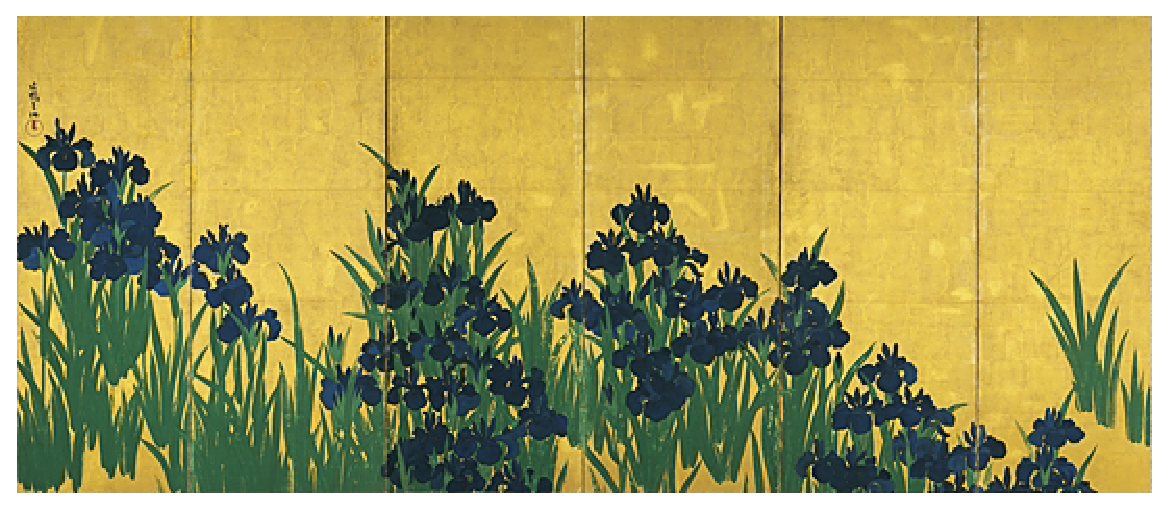
\includegraphics[scale=0.7]{irises_korin.eps}
\end{figure}
\vspace*{2cm}

\begin{flushleft}
{\large The Scalable Software Infrastructure
Project\\
{\tt http://www.ssisc.org/}}\\
\end{flushleft}
\vspace*{5mm}
\begin{flushleft}
2012$BG/(B6$B7n(B29$BF|(B
\end{flushleft}
\thispagestyle{empty}

\newpage
\begin{flushleft}
{\small
Copyright (C) 2002-2012 The Scalable Software Infrastructure Project,
supported by ``Development of Software Infrastructure for Large Scale
Scientific Simulation'' Team, CREST, JST

Akira Nishida, Research Institute for Information Technology, 
Kyushu University, 6-10-1, Hakozaki, Higashi-ku, Fukuoka 812-8581 Japan

All rights reserved.

\vspace*{5mm}
Redistribution and use in source and binary forms, with or without
modification, are permitted provided that the following conditions are
 met:

1. Redistributions of source code must retain the above copyright
 notice, 
   this list of conditions and the following disclaimer. 

2. Redistributions in binary form must reproduce the above copyright
 notice,
   this list of conditions and the following disclaimer in the
 documentation
   and/or other materials provided with the distribution. 

3. Neither the name of the University nor the names of its contributors
 may 
   be used to endorse or promote products derived from this software
 without
   specific prior written permission. 

\vspace*{5mm}
THIS SOFTWARE IS PROVIDED BY THE SCALABLE SOFTWARE INFRASTRUCTURE
 PROJECT 
``AS IS'' AND ANY EXPRESS OR IMPLIED WARRANTIES, INCLUDING, BUT NOT
 LIMITED
TO, THE IMPLIED WARRANTIES OF MERCHANTABILITY AND FITNESS FOR A
 PARTICULAR
PURPOSE ARE DISCLAIMED. IN NO EVENT SHALL THE SCALABLE SOFTWARE
 INFRASTRUCTURE
PROJECT BE LIABLE FOR ANY DIRECT, INDIRECT, INCIDENTAL, SPECIAL,
 EXEMPLARY,
OR CONSEQUENTIAL DAMAGES (INCLUDING, BUT NOT LIMITED TO, PROCUREMENT OF
SUBSTITUTE GOODS OR SERVICES; LOSS OF USE, DATA, OR PROFITS; OR BUSINESS
INTERRUPTION) HOWEVER CAUSED AND ON ANY THEORY OF LIABILITY, WHETHER IN
CONTRACT, STRICT LIABILITY, OR TORT (INCLUDING NEGLIGENCE OR OTHERWISE)
ARISING IN ANY WAY OUT OF THE USE OF THIS SOFTWARE, EVEN IF ADVISED OF
 THE
POSSIBILITY OF SUCH DAMAGE.

\vfill
$BI=;f(B: $BHx7A8wNV(B, $B1m;R2V?^(B.
}
\end{flushleft}
\thispagestyle{empty}

\newpage
\pagenumbering{roman}
\tableofcontents
%%%%%%%%%%%%%%%%%%%%%%%%%%%%%%%%%%%%%%%%%%%%%%%%%%%%%%%%%%%%%%
%%%%%%%%%%%%%%%%%%%%%%%%%%%%%%%%%%%%%%%%%%%%%%%%%%%%%%%%%%%%%%
\setcounter{section}{-1}
\newpage
 \pagenumbering{arabic}
\section{Version 1.1$B$+$i$NDI2C!&JQ99E@(B}
\begin{enumerate}
\item $B8GM-CM2rK!$rDI2C(B
\item $B%f!<%6%$%s%?%U%'!<%9$N;EMM$r0lItJQ99(B
\begin{enumerate}
\item {\tt lis\_output\_residual\_history()}, {\tt lis\_get\_residual\_history()}$B$r$=$l$>$l(B\\
{\tt lis\_solver\_output\_rhistory()}, {\tt lis\_solver\_get\_rhistory()}$B$KJQ99(B
\item Fortran$B%5%V%k!<%A%s(B{\tt lis\_vector\_set\_value()},
      {\tt lis\_vector\_get\_value()}$B$N(B\\$B%*%j%8%s$r(B1$B$KJQ99(B
\item Fortran$B%5%V%k!<%A%s(B{\tt lis\_vector\_set\_size()}$B$N%*%j%8%s$r(B1$B$KJQ99(B
\item $B1i;;@:EY$K4X$9$k%*%W%7%g%s$NL>>N$r(B{\tt -precision}$B$+$i(B{\tt -f}$B$KJQ99(B
\end{enumerate}
\end{enumerate}

\newpage
\section{$B$O$8$a$K(B}
Lis (a Library of Iterative Solvers for linear systems)$B$O(B, $BBg5,LO<BAB9TNs$r(B
$B78?t$H$9$k@~7?J}Dx<07O(B 
\[
Ax = b
\]
$B5Z$SI8=`8GM-CMLdBj(B
\[
Ax = \lambda x
\]
$B$r2r$/$?$a$NH?I|K!%i%$%V%i%j$G$"$k(B. C$B$H(BFortran$B$G5-=R$5$l$F$*$j(B, 
$BC`<!HG(B, OpenMP$B$r;HMQ$9$k6&M-%a%b%jJBNsHG(B, MPI$B$r;HMQ$9$kJ,;6%a%b%jJBNsHG$,$"$k(B. 
$BBP1~$9$k@~7?J}Dx<07O2rK!(B, $B8GM-CM2rK!$N0lMw$rI=(B\ref{tab:solvers}-\ref{tab:esolvers}, 
$BA0=hM}$rI=(B\ref{tab:precon}$B$K<($9(B. 
$B$^$?9TNs3JG<7A<0$N0lMw$rI=(B\ref{tab:storage}$B$K<($9(B. 

\begin{table}[htb]
\begin{minipage}[t]{0.30\textwidth}
\caption{$B@~7?J}Dx<07O2rK!(B} 
\vspace*{1mm}
\label{tab:solvers}
\hbox to\hsize{\hfil
\begin{tabular}{l|l}\hline\hline
CG                      & CR \\ 
BiCG                    & BiCR\cite{sogabe01} \\
CGS                     & CRS\cite{abe02} \\
BiCGSTAB                & BiCRSTAB\cite{abe02} \\
GPBiCG                  & GPBiCR\cite{abe02} \\
BiCGSafe\cite{fujino01} & BiCRSafe\cite{fujino02} \\
BiCGSTAB(l)             & TFQMR \\
Jacobi                  & Orthomin(m) \\
Gauss-Seidel            & GMRES(m) \\
SOR                     & FGMRES(m)\cite{fgmres} \\
IDR(s)\cite{idrs}       & MINRES\cite{greenbaum} \\
\hline         
\end{tabular}
\hfil}
\end{minipage}
\hspace*{12mm}
\begin{minipage}[t]{0.30\textwidth}
\caption{$B8GM-CM2rK!(B} 
\vspace*{1mm}
\label{tab:esolvers}
\hbox to\hsize{\hfil
\begin{tabular}{l}\hline\hline
Power Iteration \\
Inverse Iteration \\
Approximate Inverse Iteration \\
Rayleigh Quotient Iteration \\
Subspace Iteration \\
Lanczos Iteration \\
Conjugate Gradient\cite{knyazev,nishida1} \\
Conjugate Residual\cite{suetomi} \\
\hline         
\end{tabular}
\hfil}
\end{minipage}
\newline
\begin{minipage}[t]{0.30\textwidth}
\caption{$BA0=hM}(B} 
\vspace*{1mm}
\label{tab:precon}
\hbox to\hsize{\hfil
\begin{tabular}{l}\hline\hline
Jacobi \\
SSOR   \\
ILU(k) \\
ILUT\cite{ilut,ITSOL} \\
Crout ILU\cite{iluc,ITSOL} \\
I+S\cite{kohno01} \\
SA-AMG\cite{fujii01}  \\
Hybrid\cite{abe01} \\
SAINV\cite{bridson01}  \\
Additive Schwarz \\
$B%f!<%6Dj5A(B \\
\hline         
\end{tabular}
\hfil}
\end{minipage}
\hspace*{-4mm}
\begin{minipage}[t]{0.30\textwidth}
\caption{$B3JG<7A<0(B} 
\vspace*{1mm}
\label{tab:storage}
\hbox to\hsize{\hfil
\begin{tabular}{ll}\hline\hline
Compressed Row Storage & (CRS) \\
Compressed Column Storage & (CCS) \\
Modified Compressed Sparse Row & (MSR) \\
Diagonal &(DIA) \\
Ellpack-Itpack generalized diagonal &(ELL) \\
Jagged Diagonal &(JDS) \\
Block Sparse Row & (BSR) \\
Block Sparse Column &(BSC) \\
Variable Block Row &(VBR) \\
Dense &	(DNS) \\
Coordinate & (COO) \\
\hline         
\end{tabular}
\hfil}
\end{minipage}
\end{table}

%%%%%%%%%%%%%%%%%%%%%%%%%%%%%%%%%%%%%%%%%%%%%%%%%%%%%%%%
%%%%%%%%%%%%%%%%%%%%%%%%%%%%%%%%%%%%%%%%%%%%%%%%%%%%%%%%
%%%%%%%%%%%%%%%%%%%%%%%%%%%%%%%%%%%%%%%%%%%%%%%%%%%%%%%%%%%%%%
\section{$B%$%s%9%H!<%k(B}
$BK\@a$G$O(B, Lis$B$N%$%s%9%H!<%k(B, $B%F%9%H$N<j=g$K$D$$$F=R$Y$k(B. 
$B$J$*$3$3$G$O(BLinux$B%/%i%9%?4D6-$rA[Dj$7$F$$$k(B. 
%%%%%%%%%%%%%%%%%%%%%%%%%%%%%%%%%%%%%%
 \subsection{$BI,MW$J%7%9%F%`(B}
Lis$B$N%$%s%9%H!<%k$K$O(BC$B%3%s%Q%$%i$,I,MW$G$"$k(B. 
$B$^$?(B, Fortran$B%$%s%?%U%'!<%9$r;HMQ$9$k>l9g$O(BFortran$B%3%s%Q%$%i(B, 
AMG$BA0=hM}%k!<%A%s$r;HMQ$9$k>l9g$O(BFortran 90$B%3%s%Q%$%i$bI,MW(B
$B$H$J$k(B. $BJBNs7W;;4D6-$G$O(B, OpenMP$B$^$?$O(BMPI-1$B$r;HMQ$9$k(B. 
$BI=(B\ref{platforms}$B$K<g$JF0:n3NG'4D6-$r<($9(B
 ($BI=(B\ref{targetoption}$B$b;2>H$N$3$H(B). 

\begin{table}[htbp]
\caption{$B<g$JF0:n3NG'4D6-(B}
\label{platforms}
\begin{center}
{\small
 \begin{tabular}{l|l}
\hline
\multicolumn{1}{c|}{C$B%3%s%Q%$%i(B ($BI,?\(B) } & \multicolumn{1}{c}{OS} \\
\hline
Intel C/C++ Compiler 7.0, 8.0, 9.1, 10.1, 11.1,  & Linux \\
Intel C++ Composer XE                            & Windows  \\
\hline
IBM XL C/C++ V7.0, 9.0                     & AIX   \\
                                           & Linux \\
\hline
Sun WorkShop 6, Sun ONE Studio 7,          & Solaris \\
Sun Studio 11, 12                          &         \\
\hline
PGI C++ 6.0, 7.1, 10.5                     & Linux \\
\hline
gcc 3.3, 4.3                               & Linux \\
                                           & Mac OS X \\
                                           & Windows \\
\hline
Microsoft Visual C++ 2008, 2010            & Windows \\
\hline
\hline
\multicolumn{1}{c|}{Fortran$B%3%s%Q%$%i(B ($B%*%W%7%g%s(B) } & \multicolumn{1}{c}{OS} \\
\hline
Intel Fortran Compiler 8.1, 9.1, 10.1, 11.1, & Linux \\
Intel Fortran Composer XE                    & Windows  \\
\hline
IBM XL Fortran V9.1, 11.1                  & AIX     \\
                                           & Linux   \\
\hline
Sun WorkShop 6, Sun ONE Studio 7,          & Solaris \\
Sun Studio 11, 12                          &         \\
\hline
PGI Fortran 6.0, 7.1, 10.5                 & Linux \\
\hline
g77 3.3                                    & Linux \\
gfortran 4.3, 4.4                          & Mac OS X \\
g95 0.91                                   & Windows \\
\hline
\end{tabular}
}
\end{center}
\end{table} 
%%%%%%%%%%%%%%%%%%%%%%%%%%%%%%%%%%%%%%
 \subsection{$B%U%!%$%k$NE83+(B}
 $B<!$N%3%^%s%I$rF~NO$7$F(B, $B%U%!%$%k$rE83+$9$k(B. \verb|($VERSION)|$B$O%P!<%8%g%s$r<($9(B. \\
 \verb&      >gunzip -c lis-($VERSION).tar.gz | tar xvf - &\\
 $B$3$l$K$h$j(B, $B%G%#%l%/%H%j(B{\tt lis-(\$VERSION)}$B2<$K(B
$B?^(B\ref{listargz}$B$K<($9%5%V%G%#%l%/%H%j$,:n@.$5$l$k(B. 
%%%%%%%%%%%%%%%%%%%%%%%%%%%%%%%%%%%%%%
\begin{figure}[htbp]
\begin{center}
\small
\begin{verbatim}
lis-($VERSION)
$B('(Bconfig
$B!C(B  $B@_Dj%U%!%$%k(B
$B('(Binclude
$B!C(B  $B%X%C%@%U%!%$%k(B
$B('(Bsrc
$B!C(B  $B%=!<%9%U%!%$%k(B
$B('(Btest
$B!C(B  $B%F%9%H%W%m%0%i%`(B
$B(&(Bwin32
    Windows$B4D6-MQ$N%U%!%$%k(B
\end{verbatim}
\end{center}
\caption{{\tt lis-(\$VERSION).tar.gz}$B$N%U%!%$%k9=@.(B}
\label{listargz}
\end{figure}
%%%%%%%%%%%%%%%%%%%%%%%%%%%%%%%%%%%%%%
 \subsection{UNIX$B5Z$S8_49%7%9%F%`$N>l9g(B}
 \subsubsection{configure$B%9%/%j%W%H$N<B9T(B}
 $B<!$N%3%^%s%I$rF~NO$7$F%9%/%j%W%H$r<B9T$7(B, makefile$B$r@8@.$9$k(B. 
 \begin{itemize}
\item $B%G%U%)%k%H$N@_Dj$rMxMQ$9$k>l9g(B : \verb&      >./configure&
\item $B%$%s%9%H!<%k@h$r;XDj$9$k>l9g(B :   \verb&      >./configure --prefix=<install-dir>&
\end{itemize}
$B;XDj$G$-$k%*%W%7%g%s$rI=(B\ref{configoption}$B$K<($9(B. 
$BI=(B\ref{targetoption}$B$K(B\verb+TARGET+$B$G;XDj$G$-$k<g$J7W;;5!4D6-$r<($9(B. 
\begin{table}[htbp]
\caption{$B<g$J(Bconfigure$B%*%W%7%g%s(B ($B0lMw$O(B {\tt ./configure --help}$B$r;2>H(B) }
\label{configoption}
\begin{center}
\begin{tabular}{|l|l|}
\hline
\verb+--enable-omp+      & OpenMP$B$rMxMQ(B\\ \hline
\verb+--enable-mpi+      & MPI$B$rMxMQ(B\\ \hline
\verb+--enable-fortran+  & Fortran API$B$rMxMQ(B\\ \hline
\verb+--enable-saamg+    & SA-AMG$BA0=hM}$rMxMQ(B\\ \hline
\verb+--enable-quad+     & 4$BG\@:EY1i;;$rMxMQ(B\\ \hline
\verb+--enable-gprof+    & gprof$B$rMxMQ(B\\ \hline
\verb+--enable-shared+   & $B6&M-%i%$%V%i%j$r:n@.(B\\ \hline
\verb+--prefix=<install-dir>+    & $B%$%s%9%H!<%k@h$r;XDj(B\\ \hline
\verb+TARGET=<target>+    & $B7W;;5!4D6-$r;XDj(B\\ \hline
\verb+CC=<c_compiler>+    & C$B%3%s%Q%$%i$r;XDj(B\\ \hline
\verb+CFLAGS=<c_flags>+    & C$B%3%s%Q%$%i%*%W%7%g%s$r;XDj(B\\ \hline
\verb+FC=<fortran_compiler>+    & Fortran$B%3%s%Q%$%i$r;XDj(B\\ \hline
\verb+FCFLAGS=<fc_flags>+    & Fortran$B%3%s%Q%$%i%*%W%7%g%s$r;XDj(B\\ \hline
\verb+LDFLAGS=<ld_flags>+    & $B%j%s%/%*%W%7%g%s$r;XDj(B\\ \hline
\end{tabular}
\end{center}
\end{table}
\begin{table}[htbp]
\caption{TARGET$B$NNc(B ($B0lMw$O(B{\tt configure}$B$r;2>H(B) }
\label{targetoption}
\begin{center}
\begin{tabular}{|l|l|}
\hline
\verb+<target>+       & $B<B9T$5$l$k(Bconfigure$B%9%/%j%W%H(B \\ \hline
\verb+cray_xt3+       & \verb+./configure CC=cc FC=ftn CFLAGS="-O3 -B -fastsse -tp k8-64"+ \\
                      & \verb+  FCFLAGS="-O3 -fastsse -tp k8-64 -Mpreprocess" FCLDFLAGS="-Mnomain"+\\
                      & \verb+  ac_cv_sizeof_void_p=8 cross_compiling=yes --enable-mpi+\\
                      & \verb+  ax_f77_mangling="lower case, no underscore, extra underscore"+ \\ \hline
\verb+fujitsu_pq+     & \verb|./configure CC=fcc FC=frt ac_cv_sizeof_void_p=8| \\
                      & \verb+  CFLAGS="-O3 -Kfast,ocl,preex" FFLAGS="-O3 -Kfast,ocl,preex -Cpp"+ \\
                      & \verb+  FCFLAGS="-O3 -Kfast,ocl,preex -Cpp -Am"+\\
                      & \verb+  ax_f77_mangling="lower case, underscore, no extra underscore"+ \\ \hline
\verb+hitachi+        & \verb|./configure CC=cc FC=f90 FCLDFLAGS="-lf90s" ac_cv_sizeof_void_p=8| \\
                      & \verb+  CFLAGS="-Os -noparallel" FCFLAGS="-Oss -noparallel"+ \\
                      & \verb+  ax_f77_mangling="lower case, underscore, no extra underscore" + \\ \hline
\verb+ibm_bgl+        & \verb+./configure CC=blrts_xlc FC=blrts_xlf90+ \\
                      & \verb+  CFLAGS="-O3 -qarch=440d -qtune=440 -qstrict+ \\
                      & \verb+  -I/bgl/BlueLight/ppcfloor/bglsys/include"+ \\
                      & \verb+  FFFLAGS="-O3 -qarch=440d -qtune=440 -qsuffix=cpp=F -qfixed=72 -w+ \\
                      & \verb+  -I/bgl/BlueLight/ppcfloor/bglsys/include"+ \\
                      & \verb+  FCFLAGS="-O3 -qarch=440d -qtune=440 -qsuffix=cpp=F90 -w+ \\
                      & \verb+  -I/bgl/BlueLight/ppcfloor/bglsys/include"+ \\
                      & \verb+  ac_cv_sizeof_void_p=4 cross_compiling=yes --enable-mpi+\\
                      & \verb+  ax_f77_mangling="lower case, no underscore, no extra underscore"+ \\ \hline
\verb+nec_es+         & \verb|./configure CC=esmpic++ FC=esmpif90 AR=esar RANLIB=true | \\
                      & \verb+  ac_cv_sizeof_void_p=8 ax_vector_machine=yes cross_compiling=yes+ \\
                      & \verb+  --enable-mpi --enable-omp+ \\
                      & \verb+  ax_f77_mangling="lower case, no underscore, extra underscore"+ \\ \hline
\verb+nec_sx9_cross+  & \verb|./configure CC=sxmpic++ FC=sxmpif90 AR=sxar RANLIB=true | \\
                      & \verb+  ac_cv_sizeof_void_p=8 ax_vector_machine=yes cross_compiling=yes+ \\ 
                      & \verb+  ax_f77_mangling="lower case, no underscore, extra underscore"+ \\ \hline
\end{tabular}
\end{center}
\end{table}
%%%%%%%%%%%%%%%%%%%%%%%%%%%%%%%%%%%%%%
 \subsubsection{$B<B9T%U%!%$%k$N@8@.(B}
 {\tt lis-(\$VERSION)}$B%G%#%l%/%H%j$K$*$$$F<!$N%3%^%s%I$rF~NO$7(B, $B<B9T%U%!%$%k$r@8@.$9$k(B.\\
 \verb+      >make +\\
 $B<B9T%U%!%$%k$,@5>o$K@8@.$5$l$?$+$I$&$+$r3NG'$9$k$K$O(B, 
 {\tt lis-(\$VERSION)}$B%G%#%l%/%H%j$K$*$$$F<!$N%3%^%s%I$rF~NO$7(B, {\tt lis-(\$VERSION)/test}$B%G%#%l%/%H%j$K@8@.$5$l$?<B9T%U%!%$%k$rMQ$$$F%F%9%H$r9T$&(B. \\
 \verb+      >make check+\\
 $B$3$N%F%9%H$G$O(B, Matrix Market$B7A<0$N%U%!%$%k(B{\tt test/testmat.mtx}
 $B$+$i9TNs(B, $B%Y%/%H%k%G!<%?$rFI$_9~$_(B, $B@~7?J}Dx<07O(B$Ax=b$$B$N2r$r(B
 {\tt test/sol.txt}$B$K(B, $B$^$?<}B+MzNr$r(B{\tt test/res.txt}$B$K=q$-=P$9(B. 
 $B2r$NMWAG$,$9$Y$F(B$1$$B$J$i$P@5>o$G$"$k(B. SGI Altix 3700$B>e$G$N<B9T7k2L$r0J2<$K<($9(B. 
\begin{itembox}[l]{$B%G%U%)%k%H(B}
 \begin{minipage}{10cm}
 \begin{verbatim}
matrix size = 100 x 100 (460 nonzero entries)
initial vector x = 0
precision : double
solver    : BiCG 2
precon    : none
storage   : CRS
lis_solve : normal end

BiCG: number of iterations     = 15 (double = 15, quad = 0)
BiCG: elapsed time             = 5.178690e-03 sec.
BiCG:   preconditioner         = 1.277685e-03 sec.
BiCG:     matrix creation      = 1.254797e-03 sec.
BiCG:   linear solver          = 3.901005e-03 sec.
BiCG: relative residual 2-norm = 6.327297e-15
\end{verbatim}
\end{minipage}
\end{itembox}
\begin{itembox}[l]{{\tt --enable-omp}}
 \begin{minipage}{10cm}
 \begin{verbatim}
max number of threads = 32
number of threads = 2
matrix size = 100 x 100 (460 nonzero entries)
initial vector x = 0
precision : double
solver    : BiCG 2
precon    : none
storage   : CRS
lis_solve : normal end

BiCG: number of iterations     = 15 (double = 15, quad = 0)
BiCG: elapsed time             = 8.960009e-03 sec.
BiCG:   preconditioner         = 2.297878e-03 sec.
BiCG:     matrix creation      = 2.072096e-03 sec.
BiCG:   linear solver          = 6.662130e-03 sec.
BiCG: relative residual 2-norm = 6.221213e-15
\end{verbatim}
\end{minipage}
\end{itembox}
\begin{itembox}[l]{\tt --enable-mpi}
 \begin{minipage}{10cm}
 \begin{verbatim}
number of processes = 2
matrix size = 100 x 100 (460 nonzero entries)
initial vector x = 0
precision : double
solver    : BiCG 2
precon    : none
storage   : CRS
lis_solve : normal end

BiCG: number of iterations     = 15 (double = 15, quad = 0)
BiCG: elapsed time             = 2.911400e-03 sec.
BiCG:   preconditioner         = 1.560780e-04 sec.
BiCG:     matrix creation      = 1.459997e-04 sec.
BiCG:   linear solver          = 2.755322e-03 sec.
BiCG: relative residual 2-norm = 6.221213e-15
\end{verbatim}
\end{minipage}
\end{itembox}
\subsubsection{$B%$%s%9%H!<%k(B}
 {\tt lis-(\$VERSION)}$B%G%#%l%/%H%j$K$*$$$F<!$N%3%^%s%I$rF~NO$7(B, $B%$%s%9%H!<%k@h$N%G%#%l%/%H%j$K%U%!%$%k$r%3%T!<$9$k(B.\\
 \verb+      >make install+\\ 
\begin{verbatim}
$(INSTALLDIR)
$B('(Binclude
$B!C(B  $B(&(Blis_config.h lis.h lisf.h
$B(&(Blib
    $B(&(Bliblis.a
\end{verbatim}
{\tt lis\_config.h}$B$O%i%$%V%i%j$r@8@.$9$k:]$K(B, $B$^$?(B{\tt lis.h}$B$O(BC, {\tt lisf.h}$B$O(BFortran$B$G(B
$B%i%$%V%i%j$rMxMQ$9$k:]$KI,MW$J%X%C%@%U%!%$%k$G$"$k(B. {\tt liblis.a}$B$O@8@.$5$l$?(B
$B%i%$%V%i%j%U%!%$%k$G$"$k(B. 
%%%%%%%%%%%%%%%%%%%%%%%%%%%%%%%%%%%%%%
 \subsection{Windows$B%7%9%F%`$N>l9g(B}
{\tt lis-(\$VERSION)/win32}$B%G%#%l%/%H%j$K$"$k(BMicrosoft Visual
Studio$BMQ%=%j%e!<%7%g%s%U%!%$%k$^$?$O%W%m%8%'%/%H%U%!%$%k$N$&$A(B, $BI,MW$J$b$N$r;HMQ$9$k(B. 
{\tt lis\_with\_fortran.sln}$B$O(B
Intel Visual Fortran Compiler, {\tt lis\_with\_fortran\_mpi.sln}$B$O(BVisual
Fortran$B5Z$S(BMPICH2$B%i%$%V%i%j$rJ;MQ$9$k>l9g$N%=%j%e!<%7%g%s%U%!%$%k$G$"$k(B. 
$B%X%C%@%U%!%$%k(B $B$O(B{\tt lis-(\$VERSION)/include}$B%G%#%l%/%H%j$K3JG<$5$l$k(B. 
{\tt lis\_config\_win32.h}$B$O%i%$%V%i%j$r@8@.$9$k:]$K(B, $B$^$?(B{\tt lis.h}$B$O(BC, {\tt lisf.h}$B$O(BFortran$B$G(B
$B%i%$%V%i%j$rMxMQ$9$k:]$KI,MW$J%X%C%@%U%!%$%k$G$"$k(B. 
$B@8@.$5$l$?%i%$%V%i%j$O(B{\tt lis-(\$VERSION)/lib}$B%G%#%l%/%H%j$K3JG<$5$l$k(B. 
$B%F%9%H%W%m%0%i%`$N<B9T%U%!%$%k$O(B{\tt lis-(\$VERSION)/test}$B%G%#%l%/%H%j(B
$B$K3JG<$5$l$k(B. 
%%%%%%%%%%%%%%%%%%%%%%%%%%%%%%%%%%%%%%
\subsection{$B%F%9%H%W%m%0%i%`(B}
\subsubsection{test1}
{\tt lis-(\$VERSION)/test}$B%G%#%l%/%H%j$K$*$$$F(B\\
 \verb+      >test1 matrix_filename rhs_setting solution_filename residual_filename [options]+\\
$B$HF~NO$9$k$H(B, {\tt matrix\_filename}$B$N<($99TNs%G!<%?%U%!%$%k$+$i9TNs%G!<(B
 $B%?$rFI$_9~$_(B, 
$B@~7?J}Dx<07O(B$Ax=b$$B$r(B{\tt options}$B$G;XDj$5$l$?2rK!$G2r$/(B. $B$^$?(B, 
$B2r$r(B{\tt result\_filename}$B$K(B, $B<}B+MzNr$r(B{\tt residual\_filename}$B$K=q$-=P$9(B. 
$BF~NO2DG=$J9TNs%G!<%?7A<0$O(BMatrix Market$B7A<0$G$"$k(B. 
{\tt rhs\_setting}$B$O(B
\begin{namelist}{XXXXXXXXXXXXXXXXXXXX}
\item[0] $B9TNs%G!<%?%U%!%$%k$K4^$^$l$F$$$k1&JU%Y%/%H%k$rMQ$$$k(B
\item[1] $b = (1,\dots,1)^T$$B$rMQ$$$k(B
\item[2] $b = A \times (1,\dots,1)^T$$B$rMQ$$$k(B
\item[rhs\_filename] $B1&JU%Y%/%H%k$N%U%!%$%kL>(B
\end{namelist}
$B$,;XDj$G$-$k(B. {\tt rhs\_filename}$B$O(BPLAIN$B7A<0$^$?$O(BMatrix Market$B7A<0$,(B
$BMxMQ$G$-$k(B. 
{\tt test1f.F}$B$O(B{\tt test1.c}$B$N(BFortran$BHG$G$"$k(B. 

\subsubsection{test2}
{\tt lis-(\$VERSION)/test}$B%G%#%l%/%H%j$K$*$$$F(B\\
 \verb+      >test2 m n matrix_type solution_filename residual_filename [options]+\\
$B$HF~NO$9$k$H(B, 2$B<!85(BPoisson$BJ}Dx<0$r(B5$BE@Cf?4:9J,$GN%;62=$7$FF@$i$l$k(B
$B<!?t(B$mn$$B$N(B5$B=EBP3Q9TNs$r78?t$H$9$k(B
$B@~7?J}Dx<07O(B$Ax=b$$B$r(B, \verb|matrix_type| $B$G;XDj$5$l$?9TNs3JG<7A<0(B, 
{\tt options}$B$G;XDj$5$l$?2rK!$G2r$/(B. $B$^$?(B, 
$B2r$r(B{\tt result\_filename}$B$K<}B+MzNr$r(B{\tt residual\_filename}$B$K=q$-=P$9(B. 
$B$?$@$7(B, $B@~7?J}Dx<07O(B$Ax=b$$B$N2r%Y%/%H%k$NCM$,$9$Y$F(B$1$$B$H$J$k$h$&$K1&JU%Y%/%H%k(B$b$$B$r(B
$B@_Dj$7$F$$$k(B. $m$, $n$$B$O3F<!85$N3J;RE@?t$G$"$k(B. 

\subsubsection{test3}
{\tt lis-(\$VERSION)/test}$B%G%#%l%/%H%j$K$*$$$F(B\\
 \verb+      >test3 l m n matrix_type solution_filename residual_filename [options]+\\
$B$HF~NO$9$k$H(B, 3$B<!85(BPoisson$BJ}Dx<0$r(B7$BE@Cf?4:9J,$GN%;62=$7$FF@$i$l$k(B
$B<!?t(B$lmn$$B$N(B7$B=EBP3Q9TNs$r78?t$H$9$k(B
$B@~7?J}Dx<07O(B$Ax=b$$B$r(B, \verb|matrix_type| $B$G;XDj$5$l$?9TNs3JG<7A<0(B, 
{\tt options}$B$G;XDj$5$l$?2rK!$G2r$/(B. $B$^$?(B, 
$B2r$r(B{\tt result\_filename}$B$K<}B+MzNr$r(B{\tt residual\_filename}$B$K=q$-=P$9(B. 
$B$?$@$7(B, $B@~7?J}Dx<07O(B$Ax=b$$B$N2r%Y%/%H%k$NCM$,$9$Y$F(B$1$$B$H$J$k$h$&$K1&JU%Y%/%H%k(B$b$$B$r(B
$B@_Dj$7$F$$$k(B. $l$, $m$, $n$$B$O3F<!85$N3J;RE@?t$G$"$k(B. 

\subsubsection{test4}
$B@~7?J}Dx<07O(B$Ax=b$$B$r;XDj$5$l$?2rK!$G2r$-(B, $B2r$rI=<($9$k(B. 
$B9TNs(B$A$$B$O<!?t(B$12$$B$N(B3$B=EBP3Q9TNs(B
\[
A = 
\left(
\begin{array}{ccccc}
2 & -1 &   &  &   \\
-1 & 2 & -1 &  &   \\
  & \ddots  & \ddots  & \ddots  &   \\
  &   & -1 & 2 & -1 \\
  &   &   & -1 & 2 \\
\end{array}
\right)
\]
$B$G$"$k(B. $B1&JU%Y%/%H%k(B$b$$B$O2r(B$x$$B$,$9$Y$F(B$1$$B$H$J$k$h$&$K(B
$B5a$a$F$$$k(B. 
{\tt test4f.F}$B$O(B{\tt test4.c}$B$N(BFortran$BHG$G$"$k(B. 

\subsubsection{test5}
{\tt lis-(\$VERSION)/test}$B%G%#%l%/%H%j$K$*$$$F(B\\
 \verb+      >test5 n gamma [options]+\\
$B$HF~NO$9$k$H(B, 
$B@~7?J}Dx<07O(B$Ax=b$$B$r;XDj$5$l$?2rK!$G2r$-(B, $B2r$rI=<($9$k(B. 
$B9TNs(B$A$$B$O(BToepliz$B9TNs(B
\[
A = \left(
\begin{array}{cccccc}
2 & 1 &   &  &  & \\
0 & 2 & 1 &  &  & \\
\gamma & 0& 2 & 1 &  & \\
 & \ddots & \ddots & \ddots & \ddots & \\
 &  &   \gamma &0 &       2   & 1 \\
 &  &  &   \gamma & 0& 2 \\
\end{array}
\right)
\]
$B$G$"$k(B. $B1&JU%Y%/%H%k(B$b$$B$O2r(B$x$$B$,$9$Y$F(B$1$$B$H$J$k$h$&$K(B
$B5a$a$F$$$k(B. $n$$B$O9TNs(B$A$$B$N<!?t$G$"$k(B. 

\subsubsection{etest1}
{\tt lis-(\$VERSION)/test}$B%G%#%l%/%H%j$K$*$$$F(B\\
 \verb+      >etest1 matrix_filename solution_filename residual_filename [options]+\\
$B$HF~NO$9$k$H(B, {\tt matrix\_filename}$B$N<($99TNs%G!<%?%U%!%$%k$+$i9TNs%G!<%?$rFI$_9~$_(B, 
$B8GM-CMLdBj(B$Ax=\lambda x$$B$r(B{\tt options}$B$G;XDj$5$l$?2rK!$G2r$$$F(B, $B;XDj$5$l(B
 $B$?%b!<%I$N8GM-CM$rI=<($9$k(B. $B$^$?(B, $B8GM-CM$KBP1~$9$k8GM-%Y%/%H%k$r(B{\tt result\_filename}$B$K(B, $B<}B+MzNr$r(B{\tt residual\_filename}$B$K=q$-=P$9(B. 
$BF~NO2DG=$J9TNs%G!<%?7A<0$O(BMatrix Market$B7A<0$G$"$k(B. 
{\tt etest1f.F}$B$O(B{\tt etest1.c}$B$N(BFortran$BHG$G$"$k(B. 

\subsubsection{etest2}
{\tt lis-(\$VERSION)/test}$B%G%#%l%/%H%j$K$*$$$F(B\\
 \verb+      >etest2 m n matrix_type solution_filename residual_filename [options]+\\
$B$HF~NO$9$k$H(B, 2$B<!85(BHelmholtz$BJ}Dx<0$r(B5$BE@Cf?4:9J,$GN%;62=$7$FF@$i$l$k(B
$B<!?t(B$mn$$B$N(B5$B=EBP3Q9TNs$K4X$9$k8GM-CMLdBj(B
$Ax=\lambda x$$B$r(B, \verb|matrix_type| $B$G;XDj$5$l$?9TNs3JG<7A<0(B, 
{\tt options}$B$G;XDj$5$l$?2rK!$G2r$-(B, $B;XDj$5$l$?%b!<%I$N8GM-CM$rI=<($9$k(B. $B$^$?(B, 
$B8GM-CM$KBP1~$9$k8GM-%Y%/%H%k$r(B{\tt result\_filename}$B$K(B, $B<}B+MzNr$r(B{\tt residual\_filename}$B$K=q$-=P$9(B. 
$m$, $n$$B$O3F<!85$N3J;RE@?t$G$"$k(B. 

\subsubsection{etest3}
{\tt lis-(\$VERSION)/test}$B%G%#%l%/%H%j$K$*$$$F(B\\
 \verb+      >etest3 l m n matrix_type solution_filename residual_filename [options]+\\
$B$HF~NO$9$k$H(B, 3$B<!85(BHelmholtz$BJ}Dx<0$r(B7$BE@Cf?4:9J,$GN%;62=$7$FF@$i$l$k(B
$B<!?t(B$lmn$$B$N(B7$B=EBP3Q9TNs$K4X$9$k8GM-CMLdBj(B
$Ax=\lambda x$$B$r(B, \verb|matrix_type| $B$G;XDj$5$l$?9TNs3JG<7A<0(B, 
{\tt options}$B$G;XDj$5$l$?2rK!$G2r$-(B, $B;XDj$5$l$?%b!<%I$N8GM-CM$rI=<($9$k(B. $B$^$?(B, 
$B8GM-CM$KBP1~$9$k8GM-%Y%/%H%k$r(B{\tt result\_filename}$B$K(B, $B<}B+MzNr$r(B{\tt residual\_filename}$B$K=q$-=P$9(B. 
$l$, $m$, $n$$B$O3F<!85$N3J;RE@?t$G$"$k(B. 

\subsubsection{etest4}
{\tt lis-(\$VERSION)/test}$B%G%#%l%/%H%j$K$*$$$F(B\\
 \verb+      >etest4 n [options]+\\
$B$HF~NO$9$k$H(B, $B8GM-CMLdBj(B$Ax=\lambda x$$B$r;XDj$5$l$?2rK!$G2r$-(B, $B;XDj$5$l$?(B
 $B%b!<%I$N8GM-CM$rI=<($9$k(B. 
$B9TNs(B$A$$B$O<!?t(B$n$$B$N(B3$B=EBP3Q9TNs(B
\[
A = 
\left(
\begin{array}{ccccc}
2 & -1 &   &  &   \\
-1 & 2 & -1 &  &   \\
  & \ddots  & \ddots  & \ddots  &   \\
  &   & -1 & 2 & -1 \\
  &   &   & -1 & 2 \\
\end{array}
\right)
\]
$B$G$"$k(B. 
{\tt etest4f.F}$B$O(B{\tt etest4.c}$B$N(BFortran$BHG$G$"$k(B. 

\subsubsection{etest5}
{\tt lis-(\$VERSION)/test}$B%G%#%l%/%H%j$K$*$$$F(B\\
 \verb+      >etest5 evalue_filename evector_filename +\\
$B$HF~NO$9$k$H(B, 
$B8GM-CMLdBj(B$Ax=\lambda x$$B$r(B Subspace Iteration $B$K$h$j2r$-(B, $B@dBPCM:G>.$N(B
$B$b$N$+$i=g$K(B2$B8D$N8GM-CM$r(B{\tt evalue\_filename}$B$K(B, 
$BBP1~$9$k8GM-%Y%/%H%k$r(B
{\tt evector\_filename}$B$K3HD%(BMatrix Market$B7A<0(B
 ($BIUO?(B\ref{sec:matinp}$B$r;2>H(B) $B$G=q$-=P$9(B. 
$B9TNs(B$A$$B$O<!?t(B$12$$B$N(B3$B=EBP3Q9TNs(B
\[
A = 
\left(
\begin{array}{ccccc}
2 & -1 &   &  &   \\
-1 & 2 & -1 &  &   \\
  & \ddots  & \ddots  & \ddots  &   \\
  &   & -1 & 2 & -1 \\
  &   &   & -1 & 2 \\
\end{array}
\right)
\]
$B$G$"$k(B. 

\subsubsection{spmvtest1}
{\tt lis-(\$VERSION)/test}$B%G%#%l%/%H%j$K$*$$$F(B\\
 \verb+      >spmvtest1 n iter+\\
$B$HF~NO$9$k$H(B, 1$B<!85(BPoisson$BJ}Dx<0$r(B3$BE@Cf?4:9J,$GN%;62=$7$F(B
$BF@$i$l$k<!?t(B$n$$B$N(B3$B=EBP3Q78?t9TNs(B
\[
A = 
\left(
\begin{array}{ccccc}
2 & -1 &   &  &   \\
-1 & 2 & -1 &  &   \\
  & \ddots  & \ddots  & \ddots  &   \\
  &   & -1 & 2 & -1 \\
  &   &   & -1 & 2 \\
\end{array}
\right)
\]
$B$H%Y%/%H%k(B$(1,\dots,1)^T$$B$H$N@Q$r(B, $B<B9T2DG=$J9TNs3JG<7A<0$K$D$$$F(B
{\tt iter}$B$G;XDj$5$l$?2s?t<B9T$7(B, FLOPS$BCM$r;;=P$9$k(B. 

\subsubsection{spmvtest2}
{\tt lis-(\$VERSION)/test}$B%G%#%l%/%H%j$K$*$$$F(B\\
 \verb+      >spmvtest2 m n iter+\\
$B$HF~NO$9$k$H(B, 2$B<!85(BPoisson$BJ}Dx<0$r(B5$BE@Cf?4:9J,$GN%;62=$7$FF@$i$l$k(B
$B<!?t(B$mn$$B$N(B5$B=EBP3Q78?t9TNs$H%Y%/%H%k(B
$(1,\dots,1)^T$$B$H$N@Q$r(B, $B<B9T2DG=$J9TNs3JG<7A<0$K$D$$$F(B
{\tt iter}$B$G;XDj$5$l$?2s?t<B9T$7(B, FLOPS$BCM$r;;=P$9$k(B. 
$m$, $n$$B$O3F<!85$N3J;RE@?t$G$"$k(B. 

\subsubsection{spmvtest3}
{\tt lis-(\$VERSION)/test}$B%G%#%l%/%H%j$K$*$$$F(B\\
 \verb+      >spmvtest3 l m n iter+\\
$B$HF~NO$9$k$H(B, 3$B<!85(BPoisson$BJ}Dx<0$r(B7$BE@Cf?4:9J,$GN%;62=$7$FF@$i$l$k(B
$B<!?t(B$lmn$$B$N(B7$B=EBP3Q78?t9TNs$H%Y%/%H%k(B
$(1,\dots,1)^T$$B$H$N@Q$r(B, $B<B9T2DG=$J9TNs3JG<7A<0$K$D$$$F(B
{\tt iter}$B$G;XDj$5$l$?2s?t<B9T$7(B, FLOPS$BCM$r;;=P$9$k(B. 
$l$, $m$, $n$$B$O3F<!85$N3J;RE@?t$G$"$k(B. 

\subsubsection{spmvtest4}
{\tt lis-(\$VERSION)/test}$B%G%#%l%/%H%j$K$*$$$F(B\\
 \verb+      >spmvtest4 matrix_filename_list iter [block]+\\
$B$HF~NO$9$k$H(B, {\tt matrix\_filename\_list}$B$N<($99TNs%G!<%?(B
$B%U%!%$%k%j%9%H$+$i9TNs%G!<%?$rFI$_9~$_(B, $B3F9TNs$H%Y%/%H%k(B
$(1,\dots,1)^T$$B$H$N@Q$r<B9T2DG=$J9TNs3JG<7A<0$K$D$$$F(B
$iter$$B$G;XDj$5$l$?2s?t<B9T$7(B, FLOPS$BCM$r;;=P$9$k(B. 
$BI,MW$J$i(B$block$$B$G(BBSR, BSC$B$N%V%m%C%/%5%$%:$r;XDj$9$k(B. 

\subsubsection{spmvtest5}
{\tt lis-(\$VERSION)/test}$B%G%#%l%/%H%j$K$*$$$F(B\\
 \verb+      >spmvtest5 matrix_filename matrix_type iter [block]+\\
$B$HF~NO$9$k$H(B, {\tt matrix\_filename}$B$N<($99TNs%G!<%?%U%!%$%k(B
$B$+$i9TNs%G!<%?$rFI$_9~$_(B, $B9TNs$H%Y%/%H%k(B$(1,\dots,1)^T$$B$H$N(B
$B@Q$r9TNs3JG<7A<0(B{\tt matrix\_type}$B$K$D$$$F(B$iter$$B$G(B
$B;XDj$5$l$?2s?t<B9T$7(B, FLOPS$BCM$r;;=P$9$k(B. 
$BI,MW$J$i(B$block$$B$G(BBSR, BSC$B$N%V%m%C%/%5%$%:$r;XDj$9$k(B. 

\newpage
\subsection{$B@)8B;v9`(B}

$B8=:_$N%P!<%8%g%s$K$O0J2<$N@)8B$,$"$k(B. 
\begin{itemize}
\item $BA0=hM}(B
\begin{itemize}
\item Jacobi, SSOR$B0J30$NA0=hM}$,A*Br$5$l(B, $B$+$D9TNs(BA$B$,(BCRS$B7A<0$G$J$$>l9g(B,
      $BA0=hM}:n@.;~$K(BCRS$B7A<0$N9TNs(BA$B$,:n@.$5$l$k(B.
\item BiCG$BK!$rA*Br$7$?>l9g(B, SA-AMG$BA0=hM}$OHsBP1~(B.
\item SA-AMG$BA0=hM}$O(BOpenMP$B4D6-$KHsBP1~(B, SAINV$BA0=hM}$NA0=hM}9TNs:n@.ItJ,$OC`<!(B.
\end{itemize}

\item 4$BG\@:EY1i;;(B
\begin{itemize}
\item $B@~7?J}Dx<07O2rK!$N(BJacobi, Gauss-Seidel, SOR, IDR(s)$B$OHsBP1~(B.
\item $B8GM-CM2rK!$N(BConjugate Gradient, Conjugate Residual$B$OHsBP1~(B.
\item Hybrid$BA0=hM}$G$NFbItH?I|2rK!$N$&$A(B, Jacobi, Gauss-Seidel, SOR$B$OHsBP1~(B.
\item I+S, SA-AMG$BA0=hM}$OHsBP1~(B.
\end{itemize}

\item $B9TNs3JG<7A<0(B
\begin{itemize}
\item MPI$B4D6-$K$*$$$F%f!<%6<+?H$,I,MW$JG[Ns$rMQ0U$9$k>l9g$O(B, CRS$B7A<0$G:n(B
      $B@.$7$J$1$l$P$J$i$J$$(B.
$BL\E*$N3JG<7A<0$rMxMQ$9$k$K$O(B, \verb|lis_matrix_convert|$B$r;HMQ$7$F(B
CRS$B7A<0$+$iJQ49$9$k(B. 
\end{itemize}
\end{itemize}
\vspace*{5mm}

%%%%%%%%%%%%%%%%%%%%%%%%%%%%%%%%%%%%%%%%%%%%%%%%%%%%%%%%%%%%%%
%%%%%%%%%%%%%%%%%%%%%%%%%%%%%%%%%%%%%%%%%%%%%%%%%%%%%%%%%%%%%%
\newpage
\section{$B4pK\A`:n(B}
$BK\@a$G$O(B, $B%i%$%V%i%j$NMxMQJ}K!$K$D$$$F=R$Y$k(B. 
$B%W%m%0%i%`$G$O0J2<$N=hM}$r9T$&I,MW$,$"$k(B. 
\begin{itemize}
\item $B=i4|2==hM}(B
\item $B9TNs$N:n@.(B
\item $B%Y%/%H%k$N:n@.(B
\item $B@~7?J}Dx<07O$^$?$O8GM-CM2rK!$N$?$a$N%=%k%P(B ($B2rK!$N>pJs$r(B
      $B3JG<$9$k9=B$BN(B) $B$N:n@.(B
\item $B9TNs(B, $B%Y%/%H%k$X$NCM$NBeF~(B
\item $B2rK!$N@_Dj(B
\item $B5a2r(B
\item $B=*N;=hM}(B
\end{itemize}
$B$^$?(B, $B%W%m%0%i%`$N@hF,$K$O0J2<$N(B{\tt include}$BJ8$r5-=R$7$F$*$+$J$1$l$P$J$i$J$$(B. 
\begin{itemize}
\item \verb+C       #include "lis.h"+
\item \verb+Fortran #include "lisf.h"+
\end{itemize}
{\tt lis.h}$B$H(B{\tt lisf.h}$B$O(B\verb|$(INSTALLDIR)/include|$B$KB8:_$9$k(B. 
\newpage
\subsection{$B=i4|2=!&=*N;=hM}(B}
$B=i4|2=(B, $B=*N;=hM}$O0J2<$N$h$&$K5-=R$9$k(B. $B=i4|2==hM}$O%W%m%0%i%`$N:G=i$K(B, 
$B=*N;=hM}$O:G8e$KI,$:<B9T$7$J$1$l$P$J$i$J$$(B. 
\begin{itembox}[l]{C}
\small
\begin{verbatim}
 1: #include "lis.h"
 2: int main(int argc, char* argv[])
 3: {
 4:     lis_initialize(&argc, &argv);
 5:     ...
 6:     lis_finalize();
 7: }
\end{verbatim}
\end{itembox}
\begin{itembox}[l]{Fortran}
\small
\begin{verbatim}
 1: #include "lisf.h"
 2:      call lis_initialize(ierr) 
 3:     ...
 4:      call lis_finalize(ierr)
\end{verbatim}
\end{itembox}
\\ \\
\noindent
{\bf $B=i4|2==hM}(B}

$B=i4|2==hM}$r9T$&$K$O4X?t(B
\begin{itemize}
\item \verb+C       lis_initialize(int* argc, char** argv[])+
\item \verb+Fortran subroutine lis_initialize(integer ierr)+
\end{itemize}
$B$rMQ$$$k(B. 
$B$3$N4X?t$O(B, MPI$B$N=i4|2=(B, $B%3%^%s%I%i%$%s0z?t$N<hF@Ey$N=i4|2==hM}$r9T$&(B. 
\\ \\
\noindent
{\bf $B=*N;=hM}(B}

$B=*N;=hM}$r9T$&$K$O4X?t(B
\begin{itemize}
\item \verb+C       int lis_finalize()+
\item \verb+Fortran subroutine lis_finalize(integer ierr)+
\end{itemize}
$B$rMQ$$$k(B. 
\subsection{$B%Y%/%H%k(B}
$B%Y%/%H%k(B$v$$B$N<!?t$r(B$global\_n$$B$H$9$k(B. 
$B%Y%/%H%k(B$v$$B$r(B$nprocs$$B8D$N%W%m%;%9$G9T%V%m%C%/J,3d$7$?$H$-$N(B
$B3FItJ,%Y%/%H%k$N9T?t$r(B$local\_n$$B$H$9$k(B. 
$global\_n$$B$,(B$nprocs$$B$G3d$j@Z$l$k>l9g$O(B
$local\_n$ $=$ $global\_n$ $/$ $nprocs$$B$H$J$k(B. 
$BNc$($P(B, 
$B%Y%/%H%k(B$v$$B$r(B(\ref{eq:vecv})$B<0$N$h$&$K(B2$B%W%m%;%9$G9T%V%m%C%/J,3d$7$?>l9g(B, 
$global\_n$$B$H(B$local\_n$$B$O$=$l$>$l(B$4$$B$H(B$2$$B$H$J$k(B. 
\begin{equation}
v = 
\left(
\begin{array}{c}
0 \\
1 \\ \hline
2 \\
3  
\end{array}
\right)
\begin{array}{l}
\mbox{PE0} \\
    \\
\mbox{PE1} \\
   \\ 
\end{array}
\label{eq:vecv}
\end{equation}

(\ref{eq:vecv})$B<0$N%Y%/%H%k(B$v$$B$r:n@.$9$k>l9g(B, 
$BC`<!(B, OpenMP$BHG$G$O%Y%/%H%k(B$v$$B$=$N$b$N$r(B, MPI$BHG$G$O3F%W%m%;%9$K(B
$B%W%m%;%9?t$G9T%V%m%C%/J,3d$7$?(B
$BItJ,%Y%/%H%k$r:n@.$9$k$3$H$H$J$k(B. 

$B%Y%/%H%k(B$v$$B$r:n@.$9$k%W%m%0%i%`$O0J2<$N$h$&$K5-=R$9$k(B. $B$?$@$7(B, MPI$BHG$N(B
$B%W%m%;%9?t$O(B$2$$B$H$9$k(B. 
\begin{itembox}[l]{C ($BC`<!(B, OpenMP$BHG(B)}
\small
\begin{verbatim}
 1: int           i,n;
 2: LIS_VECTOR    v;
 3: n = 4;
 4: lis_vector_create(0,&v);
 5: lis_vector_set_size(v,0,n); /* or lis_vector_set_size(v,n,0); */ 
 6:
 7: for(i=0;i<n;i++)
 8: {
 9:     lis_vector_set_value(LIS_INS_VALUE,i,(double)i,v);
10:  }
\end{verbatim}
\end{itembox}
\begin{itembox}[l]{C (MPI$BHG(B)}
\small
\begin{verbatim}
 1: int           i,n,is,ie;                 /*or int  i,ln,is,ie;                         /*
 2: LIS_VECTOR    v;
 3: n = 4;                                   /*   ln = 2;                                  */
 4: lis_vector_create(MPI_COMM_WORLD,&v);
 5: lis_vector_set_size(v,0,n);              /*   lis_vector_set_size(v,ln,0);             */
 6: lis_vector_get_range(v,&is,&ie);
 7: for(i=is;i<ie;i++)
 8: {
 9:     lis_vector_set_value(LIS_INS_VALUE,i,(double)i,v);
10:  }
\end{verbatim}
\end{itembox}
\begin{itembox}[l]{Fortran ($BC`<!(B, OpenMP$BHG(B)}
\small
\begin{verbatim}
 1: integer       i,n
 2: LIS_VECTOR    v
 3: n = 4
 4: call lis_vector_create(0,v,ierr)
 5: call lis_vector_set_size(v,0,n,ierr)  
 6:
 7: do i=1,n
 9:     call lis_vector_set_value(LIS_INS_VALUE,i,DBLE(i),v,ierr)
10: enddo
\end{verbatim}
\end{itembox}
\begin{itembox}[l]{Fortran (MPI$BHG(B)}
\small
\begin{verbatim}
 1: integer       i,n,is,ie                 
 2: LIS_VECTOR    v
 3: n = 4                                   
 4: call lis_vector_create(MPI_COMM_WORLD,v,ierr)
 5: call lis_vector_set_size(v,0,n,ierr)              
 6: call lis_vector_get_range(v,is,ie,ierr)
 7: do i=is,ie-1
 8:     call lis_vector_set_value(LIS_INS_VALUE,i,DBLE(i),v,ierr);
 9: enddo
\end{verbatim}
\end{itembox}
\newpage
\noindent
{\bf $BJQ?t@k8@(B}

2$B9TL\$N$h$&$K(B\\
\verb|    LIS_VECTOR    v;|\\
$B$H@k8@$9$k(B. 
\\ \\
\noindent
{\bf $B%Y%/%H%k$N:n@.(B}

$B%Y%/%H%k(B$v$$B$N:n@.$O4X?t(B
\begin{itemize}
\item \verb|C       int lis_vector_create(LIS_Comm comm, LIS_VECTOR *vec)|
\item \verb|Fortran subroutine lis_vector_create(LIS_Comm comm, LIS_VECTOR vec, integer ierr)|
\end{itemize}
$B$rMQ$$$k(B. 
{\tt comm}$B$K$O(BMPI$B%3%_%e%K%1!<%?$r;XDj$9$k(B. $BC`<!(B, OpenMP$BHG$G$O(B{\tt comm}$B$NCM$OL5;k$5$l$k(B. 
\\ \\
\noindent
{\bf $B%Y%/%H%k%5%$%:$N@_Dj(B}

$B%Y%/%H%k%5%$%:$N@_Dj$O4X?t(B
\begin{itemize}
\item \verb|C       int lis_vector_set_size(LIS_VECTOR vec, int local_n, int global_n)|
\item \verb|Fortran subroutine lis_vector_set_size(LIS_VECTIR vec, integer local_n,| \\
      \verb|         integer global_n, integer ierr)|
\end{itemize}
$B$rMQ$$$k(B. 
$local\_n$ $B$+(B $global\_n$ $B$N$I$A$i$+0lJ}$rM?$($J$1$l$P$J$i$J$$(B. 

$BC`<!(B, OpenMP$BHG$G$O(B, $B%Y%/%H%k$N<!?t$O(B$local\_n$ $=$ $global\_n$$B$H$J$k(B. 
$B$7$?$,$C$F(B, \\
\verb|lis_vector_set_size(v,n,0)|
$B$H(B\verb|lis_vector_set_size(v,0,n)|$B$O$I$A$i$b<!?t(B$n$$B$N%Y%/%H%k$r:n@.$9$k$3$H$r0UL#$9$k(B. 

MPI$BHG$G$O(B, \verb|lis_vector_set_size(v,n,0)|$B$H$9$k$H(B, 
$B3F%W%m%;%9(B$p$$B$K<!?t(B$n$$B$NItJ,%Y%/%H%k$r:n@.$9$k(B. 
$B0lJ}(B, \verb|lis_vector_set_size(v,0,n)|$B$H$9$k$H(B
$B3F%W%m%;%9(B$p$$B$K<!?t(B$m_p$$B$NItJ,%Y%/%H%k$r:n@.$9$k(B. $B$?$@$7(B, $m_p$$B$NCM$O%i%$%V%i%jB&$G7hDj$5$l$k(B. 
\\ \\
\noindent
{\bf $BMWAG$NBeF~(B}

$B%Y%/%H%k(B$v$$B$N(B$i$$B9TL\$KMWAG$rBeF~$9$k$K$O4X?t(B
\begin{itemize}
\item \verb|C       int lis_vector_set_value(int flag, int i, LIS_SCALAR value, LIS_VECTOR v)|
\item \verb|Fortran subroutine lis_vector_set_value(int flag, int i, LIS_SCALAR value,|\\
      \verb|         LIS_VECTOR v, integer ierr)|
\end{itemize}
$B$rMQ$$$k(B. MPI$BHG$G$O(B, $BItJ,%Y%/%H%k$N(B$i$$B9TL\$G$O$J$/A4BN%Y%/%H%k$N(B$i$$B9TL\$r;XDj$9$k(B. 
\verb+flag+$B$K$O(B
\begin{description}
\item[\tt LIS\_INS\_VALUE] $BA^F~(B: {\tt v($i$) = $value$}
\item[\tt LIS\_ADD\_VALUE] $B2C;;BeF~(B: {\tt v($i$) = v($i$) + $value$}
\end{description}
$B$N$I$A$i$+$r;XDj$9$k(B 
\\ \\
\noindent
{\bf $B%Y%/%H%k$NJ#@=(B}

$B4{B8$N%Y%/%H%k$HF1$8>pJs$r;}$D%Y%/%H%k$r:n@.$9$k$K$O4X?t(B
\begin{itemize}
\item \verb|C       int lis_vector_duplicate(LIS_VECTOR vin, LIS_VECTOR *vout)|
\item \verb|Fortran subroutine lis_vector_duplicate(LIS_VECTOR vin, LIS_VECTOR vout,|\\
      \verb|         integer ierr)|
\end{itemize}
$B$rMQ$$$k(B. $BBh(B1$B0z?t(B\verb|LIS_VECTOR vin|$B$O(B\verb|LIS_MATRIX|$B$r;XDj$9$k$3$H$b2DG=$G$"$k(B. 
$B$3$N4X?t$O%Y%/%H%k$NMWAG$O%3%T!<$7$J$$(B. $BMWAG$b%3%T!<$7$?$$>l9g$O(B
$B$3$N4X?t$N8e$K(B
\begin{itemize}
\item \verb|C       int lis_vector_copy(LIS_VECTOR vsrc, LIS_VECTOR vdst)|
\item \verb|Fortran subroutine lis_vector_copy(LIS_VECTOR vsrc, LIS_VECTOR vdst, integer ierr)|
\end{itemize}
$B$rMQ$$$k(B. 
\\ \\
\noindent
{\bf $B%Y%/%H%k$NGK4~(B}

$BITMW$K$J$C$?%Y%/%H%k$r%a%b%j$+$iGK4~$9$k$K$O(B
\begin{itemize}
\item \verb|C       int lis_vector_destroy(LIS_VECTOR v)|
\item \verb|Fortran subroutine lis_vector_destroy(LIS_VECTOR vec, integer ierr)|
\end{itemize}
$B$rMQ$$$k(B. 
\subsection{$B9TNs(B}
$B78?t9TNs(B$A$$B$N<!?t$r(B$global\_n$ $\times$ $global\_n$$B$H$9$k(B. 
$B9TNs(B$A$$B$r(B$nprocs$$B8D$N%W%m%;%9$G9T%V%m%C%/J,3d$7$?$H$-$N(B
$B3F%V%m%C%/$N9T?t$r(B$local\_n$$B$H$9$k(B. 
$global\_n$$B$,(B$nprocs$$B$G3d$j@Z$l$k>l9g$O(B
$local\_n$ $=$ $global\_n$ $/$ $nprocs$$B$H$J$k(B. 
$BNc$($P(B, 
$B9TNs(B$A$$B$r(B(\ref{eq:mat})$B<0$N$h$&$K(B2$B8D$N%W%m%;%9$G9T%V%m%C%/J,3d$7$?>l9g(B, 
$global\_n$$B$H(B$local\_n$$B$O$=$l$>$l(B$4$$B$H(B$2$$B$H$J$k(B. 
\begin{equation}
\label{eq:mat}
A = 
\left(
\begin{array}{cccc}
2 & 1 &   &    \\
1 & 2 & 1 &    \\ \hline
  & 1 & 2 & 1 \\
  &   & 1 & 2 
\end{array}
\right)
\begin{array}{l}
\mbox{PE0} \\
    \\
\mbox{PE1} \\
   \\ 
\end{array}
\end{equation}

$BL\E*$N3JG<7A<0$N9TNs$r:n@.$9$k$K$O0J2<$N(B3$B$D$NJ}K!$,$"$k(B.\\ \\
\noindent
{\bf $BJ}K!(B1: $B%i%$%V%i%j4X?t$rMQ$$$FL\E*$N3JG<7A<0$KI,MW$JG[Ns$rDj5A$9$k>l9g(B}\\
(\ref{eq:mat})$B<0$N9TNs(B$A$$B$r(BCRS$B7A<0$G:n@.$9$k>l9g(B, 
$BC`<!(B, OpenMP$BHG$G$O9TNs(B$A$$B$=$N$b$N$r(B, MPI$BHG$G$O3F%W%m%;%9$K(B
$B%W%m%;%9?t$G9T%V%m%C%/J,3d$7$?(B
$BItJ,9TNs$r:n@.$9$k$3$H$H$J$k(B. 

$B9TNs(B$A$$B$r(BCRS$B7A<0$G:n@.$9$k%W%m%0%i%`$O0J2<$N$h$&$K5-=R$9$k(B. 
$B$?$@$7(B, MPI$BHG$N%W%m%;%9?t$O(B$2$$B$H$9$k(B. 
\begin{itembox}[l]{C ($BC`<!(B, OpenMP$BHG(B)}
\small
\begin{verbatim}
 1: int           i,n;
 2: LIS_MATRIX    A;
 3: n = 4;
 4: lis_matrix_create(0,&A);
 5: lis_matrix_set_size(A,0,n); /* or lis_matrix_set_size(A,n,0); */ 
 6: for(i=0;i<n;i++) {
 7:     if( i>0   ) lis_matrix_set_value(LIS_INS_VALUE,i,i-1,1.0,A);
 8:     if( i<n-1 ) lis_matrix_set_value(LIS_INS_VALUE,i,i+1,1.0,A);
 9:     lis_matrix_set_value(LIS_INS_VALUE,i,i,2.0,A);
10:  }
11:  lis_matrix_set_type(A,LIS_MATRIX_CRS);
12:  lis_matrix_assemble(A);
\end{verbatim}
\end{itembox}
\begin{itembox}[l]{C (MPI$BHG(B)}
\small
\begin{verbatim}
 1: int           i,n,gn,is,ie;                 
 2: LIS_MATRIX    A;
 3: gn = 4;                                  /* or n=2                         */
 4: lis_matrix_create(MPI_COMM_WORLD,&A);
 5: lis_matrix_set_size(A,0,gn);             /*    lis_matrix_set_size(A,n,0); */
 6: lis_matrix_get_size(A,&n,&gn);
 7: lis_matrix_get_range(A,&is,&ie);
 8: for(i=is;i<ie;i++) {
 9:     if( i>0    ) lis_matrix_set_value(LIS_INS_VALUE,i,i-1,1.0,A);
10:     if( i<gn-1 ) lis_matrix_set_value(LIS_INS_VALUE,i,i+1,1.0,A);
11:     lis_matrix_set_value(LIS_INS_VALUE,i,i,2.0,A);
12:  }
13:  lis_matrix_set_type(A,LIS_MATRIX_CRS);
14:  lis_matrix_assemble(A);
\end{verbatim}
\end{itembox}
\begin{itembox}[l]{Fortran ($BC`<!(B, OpenMP$BHG(B)}
\small
\begin{verbatim}
 1: integer       i,n
 2: LIS_MATRIX    A
 3: n = 4
 4: call lis_matrix_create(0,A,ierr)
 5: call lis_matrix_set_size(A,0,n,ierr)
 6: do i=1,n
 7:     if( i>1 ) call lis_matrix_set_value(LIS_INS_VALUE,i,i-1,1.0d0,A,ierr)
 8:     if( i<n ) call lis_matrix_set_value(LIS_INS_VALUE,i,i+1,1.0d0,A,ierr)
 9:     call lis_matrix_set_value(LIS_INS_VALUE,i,i,2.0d0,A,ierr)
10:  enddo
11:  call lis_matrix_set_type(A,LIS_MATRIX_CRS,ierr)
12:  call lis_matrix_assemble(A,ierr)
\end{verbatim}
\end{itembox}
\begin{itembox}[l]{Fortran (MPI$BHG(B)}
\small
\begin{verbatim}
 1: integer       i,n,gn,is,ie                 
 2: LIS_MATRIX    A
 3: gn = 4
 4: call lis_matrix_create(MPI_COMM_WORLD,A,ierr)
 5: call lis_matrix_set_size(A,0,gn,ierr)
 6: call lis_matrix_get_size(A,n,gn,ierr)
 7: call lis_matrix_get_range(A,is,ie,ierr)
 8: do i=is,ie-1
 9:     if( i>1  ) call lis_matrix_set_value(LIS_INS_VALUE,i,i-1,1.0d0,A,ierr)
10:     if( i<gn ) call lis_matrix_set_value(LIS_INS_VALUE,i,i+1,1.0d0,A,ierr)
11:     call lis_matrix_set_value(LIS_INS_VALUE,i,i,2.0d0,A,ierr)
12:  enddo
13:  call lis_matrix_set_type(A,LIS_MATRIX_CRS,ierr)
14:  call lis_matrix_assemble(A,ierr)
\end{verbatim}
\end{itembox}
\\ \\
\noindent
{\bf $BJQ?t@k8@(B}

2$B9TL\$N$h$&$K(B\\
\verb|    LIS_MATRIX    A;|\\
$B$H@k8@$9$k(B. 
\\ \\
\noindent
{\bf $B9TNs$N:n@.(B}

$B9TNs(B$A$$B$N:n@.$O4X?t(B
\begin{itemize}
\item \verb|C       int lis_matrix_create(LIS_Comm comm, LIS_MATRIX *A)|
\item \verb|Fortran subroutine lis_matrix_create(LIS_Comm comm, LIS_MATRIX A, integer ierr)|
\end{itemize}
$B$rMQ$$$k(B. 
{\tt comm}$B$K$O(BMPI$B%3%_%e%K%1!<%?$r;XDj$9$k(B. $BC`<!(B, OpenMP$BHG$G$O(B, {\tt comm}$B$NCM$OL5;k$5$l$k(B. 
\\ \\
\noindent
{\bf $B9TNs$N%5%$%:@_Dj(B}

$B9TNs(B$A$$B$N%5%$%:@_Dj$O4X?t(B
\begin{itemize}
\item \verb|C       int lis_matrix_set_size(LIS_MATRIX A, int local_n, int global_n)|
\item \verb|Fortran subroutine lis_matrix_set_size(LIS_MATRIX A, integer local_n,|\\
      \verb|         integer global_n, integer ierr)|
\end{itemize}
$B$rMQ$$$k(B. 
$local\_n$ $B$+(B $global\_n$ $B$N$I$A$i$+0lJ}$rM?$($J$1$l$P$J$i$J$$(B. 

$BC`<!(B, OpenMP$BHG$G$O(B, $B9TNs$N%5%$%:$O(B$local\_n$ $=$ $global\_n$$B$H$J$k(B. 
$B$7$?$,$C$F(B, \\
\verb|lis_matrix_set_size(A,n,0)|
$B$H(B\verb|lis_matrix_set_size(A,0,n)|$B$O$H$b$K(B$n \times n$$B$N%5%$%:$r@_Dj$9$k$3$H$r0UL#$9$k(B. 

MPI$BHG$G$O(B, \verb|lis_matrix_set_size(A,n,0)|$B$H$9$k$H(B, 
$B3F%W%m%;%9(B$p$$B$G9TNs%5%$%:$,(B$n_p \times N$$B$H$J$k$h$&$K@_Dj$9$k(B. $B$3$3$G(B, $N$
$B$O3F%W%m%;%9$N(B$n_p$$B$N(B
$BAmOB$G$"$k(B. \\
$B0lJ}(B, \verb|lis_matrix_set_size(A,0,n)|$B$H$9$k$H(B
$B3F%W%m%;%9(B$p$$B$G9TNs%5%$%:$,(B$m_p \times n$$B$H$J$k$h$&$K@_Dj$9$k(B. $B$3$3$G(B, $m_p$$B$OItJ,9TNs$N9T?t$G(B
$B$3$NCM$O%i%$%V%i%jB&$G7hDj$5$l$k(B. 
\\ \\
\noindent
{\bf $BMWAG$NBeF~(B}

$B9TNs(B$A$$B$N(B$i$$B9T(B$j$$BNsL\$KMWAG$rBeF~$9$k$K$O4X?t(B
\begin{itemize}
\item \verb|C       int lis_matrix_set_value(int flag, int i, int j, LIS_SCALAR value,|\\
      \verb|         LIS_MATRIX A)|
\item \verb|Fortran subroutine lis_matrix_set_value(integer flag, integer i, integer j,|\\
      \verb|         LIS_SCALAR value, LIS_MATRIX A, integer ierr)|
\end{itemize}
$B$rMQ$$$k(B. MPI$BHG$G$O(B, $BItJ,9TNs$N(B$i$$B9T(B$j$$BNsL\$G$O$J$/A4BN9TNs$N(B$i$$B9T(B$j$$BNsL\$r;XDj$9$k(B. 
flag$B$K$O(B
\begin{description}
\item[\tt LIS\_INS\_VALUE] $BA^F~(B: $A(i,j) = value$
\item[\tt LIS\_ADD\_VALUE] $B2C;;BeF~(B: $A(i,j) = A(i,j) + value$
\end{description}
$B$N$I$A$i$+$r;XDj$9$k(B 
\\ \\
\noindent
{\bf $B9TNs3JG<7A<0$N@_Dj(B}

$B9TNs$N3JG<7A<0$r@_Dj$9$k$K$O4X?t(B
\begin{itemize}
\item \verb|C       int lis_matrix_set_type(LIS_MATRIX A, int matrix_type)|
\item \verb|Fortran subroutine lis_matrix_set_type(LIS_MATRIX A, int matrix_type, integer ierr)|
\end{itemize}
$B$rMQ$$$k(B. 
$B9TNs:n@.;~$K(B $A$ $B$N(B \verb+matrix_type+ $B$O(B \verb+LIS_MATRIX_CRS+ $B$H$J$C$F$$$k(B. 
$B0J2<$K(B \verb+matrix_type+ $B$K;XDj2DG=$J3JG<7A<0$r<($9(B. 
\\ \\
\begin{minipage}[t]{\textwidth}
\begin{center}
\begin{tabular}{lll}\hline\hline
$B3JG<7A<0(B  & & matrix\_type \\ \hline
Compressed Row Storage & (CRS) & \verb={LIS_MATRIX_CRS|1}= \\
Compressed Column Storage & (CCS) & \verb={LIS_MATRIX_CCS|2}= \\
Modified Compressed Sparse Row & (MSR) & \verb={LIS_MATRIX_MSR|3}= \\
Diagonal &(DIA) & \verb={LIS_MATRIX_DIA|4}= \\
Ellpack-Itpack generalized diagonal &(ELL) & \verb={LIS_MATRIX_ELL|5}= \\
Jagged Diagonal &(JDS) & \verb={LIS_MATRIX_JDS|6}= \\
Block Sparse Row & (BSR) & \verb={LIS_MATRIX_BSR|7}= \\
Block Sparse Column &(BSC) & \verb={LIS_MATRIX_BSC|8}= \\
Variable Block Row &(VBR) & \verb={LIS_MATRIX_VBR|9}= \\
Dense &	(DNS) & \verb={LIS_MATRIX_DNS|10}= \\
Coordinate & (COO) & \verb={LIS_MATRIX_COO|11}= \\
\hline         
\end{tabular}
\end{center}
\end{minipage}
\\ \\
\noindent
{\bf $B9TNs$NAH$_N)$F(B}

$B9TNs$NMWAG$r$9$Y$FBeF~$7$?$i(B, $BI,$:4X?t(B
\begin{itemize}
\item \verb|C       int lis_matrix_assemble(LIS_MATRIX A)|
\item \verb|Fortran subroutine lis_matrix_assemble(LIS_MATRIX A, integer ierr)|
\end{itemize}
$B$r8F$S=P$9(B. 
\verb|lis_matrix_assemble| $B$O(B \verb|lis_matrix_set_type| $B$G;XDj$5$l$?3JG<7A<0$KAH$_N)$F$i$l$k(B. 
\\ \\ \\
\noindent
{\bf $B9TNs$NGK4~(B}

$BITMW$K$J$C$?9TNs$r%a%b%j$+$iGK4~$9$k$K$O(B
\begin{itemize}
\item \verb|C       int lis_matrix_destroy(LIS_MATRIX A)|
\item \verb|Fortran subroutine lis_matrix_destroy(LIS_MATRIX A, integer ierr)|
\end{itemize}
$B$rMQ$$$k(B. 
\\ \\
{\bf $BJ}K!(B2: $BL\E*$N3JG<7A<0$KI,MW$JG[Ns$rD>@\Dj5A$9$k>l9g(B}\\
(\ref{eq:mat})$B<0$N9TNs(B$A$$B$r(BCRS$B7A<0$G:n@.$9$k>l9g(B, 
$BC`<!(B, OpenMP$BHG$G$O9TNs(B$A$$B$=$N$b$N$r(B, MPI$BHG$G$O3F%W%m%;%9$K(B
$B%W%m%;%9?t$G9T%V%m%C%/J,3d$7$?(B
$BItJ,9TNs$r:n@.$9$k$3$H$H$J$k(B. 

$B9TNs(B$A$$B$r(BCRS$B7A<0$G:n@.$9$k%W%m%0%i%`$O0J2<$N$h$&$K5-=R$9$k(B. 
$B$?$@$7(B, MPI$BHG$N%W%m%;%9?t$O(B$2$$B$H$9$k(B. 
\begin{itembox}[l]{C ($BC`<!(B, OpenMP$BHG(B)}
\small
\begin{verbatim}
 1: int           i,k,n,nnz;
 2: int           *ptr,*index;
 3: LIS_SCALAR    *value;
 4: LIS_MATRIX    A;
 5: n = 4; nnz = 10; k = 0;
 6: lis_matrix_malloc_crs(n,nnz,&ptr,&index,&value);
 7: lis_matrix_create(0,&A);
 8: lis_matrix_set_size(A,0,n);  /* or lis_matrix_set_size(A,n,0); */ 
 9: 
10: for(i=0;i<n;i++)
11: {
12:     if( i>0   ) {index[k] = i-1; value[k] = 1; k++;}
13:     index[k] = i; value[k] = 2; k++;
14:     if( i<n-1 ) {index[k] = i+1; value[k] = 1; k++;}
15:     ptr[i+1] = k;
16:  }
17:  ptr[0] = 0;
18:  lis_matrix_set_crs(nnz,ptr,index,value,A);
19:  lis_matrix_assemble(A); 


\end{verbatim}
\end{itembox}
\begin{itembox}[l]{C (MPI$BHG(B)}
\small
\begin{verbatim}
 1: int           i,k,n,nnz,is,ie;
 2: int           *ptr,*index;
 3: LIS_SCALAR    *value;
 4: LIS_MATRIX    A;
 5: n = 2; nnz = 5; k = 0;
 6: lis_matrix_malloc_crs(n,nnz,&ptr,&index,&value);
 7: lis_matrix_create(MPI_COMM_WORLD,&A);
 8: lis_matrix_set_size(A,n,0);
 9: lis_matrix_get_range(A,&is,&ie);
10: for(i=is;i<ie;i++)
11: {
12:     if( i>0   ) {index[k] = i-1; value[k] = 1; k++;}
13:     index[k] = i; value[k] = 2; k++;
14:     if( i<n-1 ) {index[k] = i+1; value[k] = 1; k++;}
15:     ptr[i-is+1] = k;
16:  }
17:  ptr[0] = 0;
18:  lis_matrix_set_crs(nnz,ptr,index,value,A);
19:  lis_matrix_assemble(A); 
\end{verbatim}
\end{itembox}
\\ \\
\noindent
{\bf $BG[Ns$N4XO"IU$1(B}

$B%f!<%6<+?H$,:n@.$7$?(BCRS$B7A<0$KI,MW$JG[Ns$r%i%$%V%i%j$,07$($k$h$&9TNs(B$A$$B$K(B
$B4XO"IU$1$k$K$O(B, $B4X?t(B
\begin{itemize}
\item \verb|C       int lis_matrix_set_crs(int nnz, int row[], int index[], LIS_SCALAR value[],|\\
      \verb|         LIS_MATRIX A)|
\item \verb|Fortran subroutine lis_matrix_set_crs(integer nnz, integer row(), integer index(),|\\
      \verb|         LIS_SCALAR value(), LIS_MATRIX A, integer ierr)|
\end{itemize}
$B$rMQ$$$k(B. 
$B$=$NB>$N3JG<7A<0$K$D$$$F$OBh(B\ref{sec:storages}$B@a$r;2>H$;$h(B. 
\\ \\
{\bf $BJ}K!(B3: $B30It%U%!%$%k$+$i9TNs(B, $B%Y%/%H%k%G!<%?$rFI$_9~$`>l9g(B}\\
$B30It%U%!%$%k$+$i(B(\ref{eq:mat})$B<0$N9TNs(B$A$$B$r(BCRS$B7A<0$GFI$_9~$`>l9g$N%W%m%0%i%`$O0J2<$N$h$&$K5-=R$9$k(B. 
\begin{itembox}[l]{C ($BC`<!(B, OpenMP, MPI$BHG(B)}
\small
\begin{verbatim}
 1: LIS_MATRIX    A;
 3: lis_matrix_create(LIS_COMM_WORLD,&A); 
 6: lis_matrix_set_type(A,LIS_MATRIX_CRS); 
 7: lis_input_matrix(A,"matvec.mtx"); 
\end{verbatim}
\end{itembox}
\begin{itembox}[l]{Fortran ($BC`<!(B, OpenMP, MPI$BHG(B)}
\small
\begin{verbatim}
 1: LIS_MATRIX    A
 3: call lis_matrix_create(LIS_COMM_WORLD,A,ierr) 
 6: call lis_matrix_set_type(A,LIS_MATRIX_CRS,ierr) 
 7: call lis_input_matrix(A,'matvec.mtx',ierr) 
\end{verbatim}
\end{itembox}
\\ \\
Matrix Market$B7A<0$K$h$k30It%U%!%$%k(B{\tt matvec.mtx}$B$N5-=RNc$r0J2<$K<($9(B. 
{\small
\begin{verbatim}
%%MatrixMarket matrix coordinate real general
4 4 10 1 0
1 2  1.0e+00
1 1  2.0e+00
2 3  1.0e+00
2 1  1.0e+00
2 2  2.0e+00
3 4  1.0e+00
3 2  1.0e+00
3 3  2.0e+00
4 4  2.0e+00
4 3  1.0e+00
\end{verbatim}
}

$B30It%U%!%$%k$+$i(B(\ref{eq:mat})$B<0$N9TNs(B$A$$B$r(BCRS$B7A<0$G(B, $B$^$?(B(\ref{eq:vecv})$B<0$N%Y%/%H%k(B$b$$B$rFI$_9~$`(B
$B>l9g$N%W%m%0%i%`$O0J2<$N$h$&$K5-=R$9$k(B. 
\begin{itembox}[l]{C ($BC`<!(B, OpenMP, MPI$BHG(B)}
\small
\begin{verbatim}
 1: LIS_MATRIX    A;
 2: LIS_VECTOR    b,x;
 3: lis_matrix_create(LIS_COMM_WORLD,&A); 
 4: lis_vector_create(LIS_COMM_WORLD,&b); 
 5: lis_vector_create(LIS_COMM_WORLD,&x); 
 6: lis_matrix_set_type(A,LIS_MATRIX_CRS); 
 7: lis_input(A,b,x,"matvec.mtx"); 
\end{verbatim}
\end{itembox}
\begin{itembox}[l]{Fortran ($BC`<!(B, OpenMP, MPI$BHG(B)}
\small
\begin{verbatim}
 1: LIS_MATRIX    A
 2: LIS_VECTOR    b,x
 3: call lis_matrix_create(LIS_COMM_WORLD,A,ierr) 
 4: call lis_vector_create(LIS_COMM_WORLD,b,ierr) 
 5: call lis_vector_create(LIS_COMM_WORLD,x,ierr) 
 6: call lis_matrix_set_type(A,LIS_MATRIX_CRS,ierr) 
 7: call lis_input(A,b,x,'matvec.mtx',ierr) 
\end{verbatim}
\end{itembox}
\\ \\
$B3HD%(BMatrix Market$B7A<0$K$h$k30It%U%!%$%k(B{\tt matvec.mtx}$B$N5-=RNc$r0J2<$K(B
$B<($9(B ($BIUO?(B\ref{sec:matinp}$B$r;2>H(B). 
{\small
\begin{verbatim}
%%MatrixMarket matrix coordinate real general
4 4 10 1 0
1 2  1.0e+00
1 1  2.0e+00
2 3  1.0e+00
2 1  1.0e+00
2 2  2.0e+00
3 4  1.0e+00
3 2  1.0e+00
3 3  2.0e+00
4 4  2.0e+00
4 3  1.0e+00
1  0.0e+00
2  1.0e+00
3  2.0e+00
4  3.0e+00
\end{verbatim}
}

\noindent
{\bf $B30It%U%!%$%k$+$i$NFI$_9~$_(B}

$B30It%U%!%$%k$+$i9TNs(B$A$$B$N%G!<%?$rFI$_9~$`$K$O(B, $B4X?t(B
\begin{itemize}
\item \verb|C       int lis_input_matrix(LIS_MATRIX A, char *filename)|
\item \verb|Fortran subroutine lis_input_matrix(LIS_MATRIX A, |\\
      \verb|         character filename, integer ierr)|
\end{itemize}
$B$rMQ$$$k(B. {\tt filename}$B$K$O%U%!%$%k%Q%9$r;XDj$9$k(B. 
$BBP1~$9$k%U%!%$%k7A<0$O0J2<$NDL$j$G$"$k(B ($B%U%!%$%k7A<0$K$D$$$F$OIUO?(B\ref{sec:matinp}$B$r;2>H(B). 
\begin{itemize}
\item Matrix Market$B7A<0(B
\item Harwell-Boeing$B7A<0(B
\end{itemize}

$B30It%U%!%$%k$+$i9TNs(B$A$$B$H%Y%/%H%k(B$b$, $x$$B$N%G!<%?$rFI$_9~$`$K$O(B, $B4X?t(B
\begin{itemize}
\item \verb|C       int lis_input(LIS_MATRIX A, LIS_VECTOR b, LIS_VECTOR x, char *filename)|
\item \verb|Fortran subroutine lis_input(LIS_MATRIX A, LIS_VECTOR b, LIS_VECTOR x,|\\
      \verb|         character filename, integer ierr)|
\end{itemize}
$B$rMQ$$$k(B. {\tt filename}$B$K$O%U%!%$%k%Q%9$r;XDj$9$k(B. 
$BBP1~$9$k%U%!%$%k7A<0$O0J2<$NDL$j$G$"$k(B ($B%U%!%$%k7A<0$K$D$$$F$OIUO?(B\ref{sec:matinp}$B$r;2>H(B). 
\begin{itemize}
\item $B3HD%(BMatrix Market$B7A<0(B ($B%Y%/%H%k%G!<%?$KBP1~(B) 
\item Harwell-Boeing$B7A<0(B
\end{itemize}

\subsection{$B@~7?J}Dx<07O$N5a2r(B}\label{subsec:solve}
$B@~7?J}Dx<07O(B$Ax=b$$B$r;XDj$5$l$?2rK!$G2r$/%W%m%0%i%`$O0J2<$N$h$&$K5-=R$9$k(B. 
\begin{itembox}[l]{C ($BC`<!(B, OpenMP, MPI$BHG(B)}
\small
\begin{verbatim}
 1: LIS_MATRIX A; 
 2: LIS_VECTOR b,x; 
 3: LIS_SOLVER solver; 
 4:    
 5: /* $B9TNs$H%Y%/%H%k$N:n@.(B */ 
 6:    
 7: lis_solver_create(&solver); 
 8: lis_solver_set_option("-i bicg -p none",solver); 
 9: lis_solver_set_option("-tol 1.0e-12",solver); 
10: lis_solve(A,b,x,solver); 
\end{verbatim}
\end{itembox}
\begin{itembox}[l]{Fortran ($BC`<!(B, OpenMP, MPI$BHG(B)}
\small
\begin{verbatim}
 1: LIS_MATRIX A 
 2: LIS_VECTOR b,x 
 3: LIS_SOLVER solver 
 4:    
 5: /* $B9TNs$H%Y%/%H%k$N:n@.(B */ 
 6:    
 7: call lis_solver_create(solver,ierr) 
 8: call lis_solver_set_option('-i bicg -p none',solver,ierr) 
 9: call lis_solver_set_option('-tol 1.0e-12',solver,ierr) 
10: call lis_solve(A,b,x,solver,ierr) 
\end{verbatim}
\end{itembox}
\\ \\
\noindent
{\bf $B%=%k%P$N:n@.(B}

$B%=%k%P(B ($B@~7?J}Dx<07O2rK!$N>pJs$r3JG<$9$k9=B$BN(B) $B$r:n@.$9$k$K$O4X?t(B
\begin{itemize}
\item \verb|C       int lis_solver_create(LIS_SOLVER *solver)|
\item \verb|Fortran subroutine lis_solver_create(LIS_SOLVER solver, integer ierr) |
\end{itemize}
$B$rMQ$$$k(B. 
\\ \\
\noindent
{\bf $B%*%W%7%g%s$N@_Dj(B}

$B@~7?J}Dx<07O2rK!$r%=%k%P$K@_Dj$9$k$K$O4X?t(B 
\begin{itemize}
\item \verb|C       int lis_solver_set_option(char *text, LIS_SOLVER solver)|
\item \verb|Fortran subroutine lis_solver_set_option(character text, LIS_SOLVER solver,|\\
      \verb|         integer ierr)|
\end{itemize}
$B$^$?$O(B
\begin{itemize}
\item \verb|C       int lis_solver_set_optionC(LIS_SOLVER solver)|
\item \verb|Fortran subroutine lis_solver_set_optionC(LIS_SOLVER solver, integer ierr)|
\end{itemize}
$B$rMQ$$$k(B. 
\verb|lis_solver_set_optionC|$B$O%f!<%6%W%m%0%i%`<B9T;~$K%3%^%s%I%i%$%s$G(B
$B;XDj$5$l$?%*%W%7%g%s$r%=%k%P$K@_Dj$9$k4X?t$G$"$k(B. 

$B0J2<$K;XDj2DG=$J%3%^%s%I%i%$%s%*%W%7%g%s$r<($9(B. \verb=-i {cg|1}=$B$O(B\verb=-i cg=$B$^$?$O(B\verb=-i 1=
$B$r0UL#$9$k(B. \\
\verb=-maxiter [1000]=$B$O(B\verb=-maxiter=$B$N%G%U%)%k%HCM$,(B$1000$$B$G$"$k$3$H$r0UL#$9$k(B. 
\\
\\
\begin{minipage}[t]{\textwidth}
\begin{center}
{\bf $B@~7?J}Dx<07O2rK!$N;XDj(B} $B%G%U%)%k%H(B: \verb=-i bicg= \\
\begin{tabular}{l|lll}\hline\hline
 $B@~7?J}Dx<07O2rK!(B        & $B%*%W%7%g%s(B              &  $BJd=u%*%W%7%g%s(B  & \\ \hline
 CG          & \verb=-i {cg|1}=         &    \\ 
 BiCG        & \verb=-i {bicg|2}=       &    \\
 CGS         & \verb=-i {cgs|3}=        &    \\
 BiCGSTAB    & \verb=-i {bicgstab|4}=   &    \\
 BiCGSTAB(l) & \verb=-i {bicgstabl|5}=  & \verb=-ell [2]=      & $B<!?t(B$l$ \\
 GPBiCG      & \verb=-i {gpbicg|6}=     &    \\
 TFQMR       & \verb=-i {tfqmr|7}=      &    \\
 Orthomin(m) & \verb=-i {orthomin|8}=   & \verb=-restart [40]= & $B%j%9%?!<%HCM(B$m$  \\
 GMRES(m)    & \verb=-i {gmres|9}=      & \verb=-restart [40]= & $B%j%9%?!<%HCM(B$m$  \\ 
 Jacobi      & \verb=-i {jacobi|10}=    &    \\
 Gauss-Seidel& \verb=-i {gs|11}=        &    \\
 SOR         & \verb=-i {sor|12}=       & \verb=-omega [1.9]=  & $B4KOB78?t(B$\omega$ ($0<\omega<2$) \\
 BiCGSafe    & \verb=-i {bicgsafe|13}=  &    \\
 CR          & \verb=-i {cr|14}=        &    \\ 
 BiCR        & \verb=-i {bicr|15}=      &    \\
 CRS         & \verb=-i {crs|16}=       &    \\
 BiCRSTAB    & \verb=-i {bicrstab|17}=  &    \\
 GPBiCR      & \verb=-i {gpbicr|18}=    &    \\
 BiCRSafe    & \verb=-i {bicrsafe|19}=  &    \\
 FGMRES(m)   & \verb=-i {fgmres|20}=    & \verb=-restart [40]= & $B%j%9%?!<%HCM(B$m$  \\ 
 IDR(s)      & \verb=-i {idrs|21}=      & \verb=-irestart [2]= & $B%j%9%?!<%HCM(B$s$  \\ 
 MINRES      & \verb=-i {minres|22}=    &    \\
\hline         
\end{tabular}
\end{center}
\end{minipage}
\\ \\
\begin{minipage}[t]{\textwidth}
\begin{center}
{\bf $BA0=hM}$N;XDj(B} $B%G%U%)%k%H(B: \verb=-p none=\\
\begin{tabular}{l|lll}\hline\hline
$BA0=hM}(B   & $B%*%W%7%g%s(B           & $BJd=u%*%W%7%g%s(B \\ \hline
$B$J$7(B     & \verb=-p {none|0}=    &   \\
Jacobi   & \verb=-p {jacobi|1}=  &     \\
ILU(k)   & \verb=-p {ilu|2}=     & \verb=-ilu_fill [0]=    & $B%U%#%k%$%s%l%Y%k(B$k$ \\
SSOR     & \verb=-p {ssor|3}=    & \verb=-ssor_w [1.0]=    & $B4KOB78?t(B$\omega$ ($0<\omega<2$) \\
Hybrid   & \verb=-p {hybrid|4}=  & \verb=-hybrid_i [sor]=  & $B@~7?J}Dx<07O2rK!(B \\
         &                       & \verb=-hybrid_maxiter [25]= & $B:GBgH?I|2s?t(B \\
         &                       & \verb=-hybrid_tol [1.0e-3]= & $B<}B+H=Dj4p=`(B \\
         &                       & \verb=-hybrid_w [1.5]=      & SOR$B$N4KOB78?t(B$\omega$ ($0<\omega<2$) \\
         &                       & \verb=-hybrid_ell [2]=      & BiCGSTAB(l)$B$N<!?t(B$l$\\
         &                       & \verb=-hybrid_restart [40]= & GMRES(m), Orthomin(m)$B$N(B \\
         &                       &                             & $B%j%9%?!<%HCM(B$m$ \\
I+S      & \verb=-p {is|5}=      & \verb=-is_alpha [1.0]=  & $I+\alpha S^{(m)}$$B7?A0=hM}$N%Q%i%a!<%?(B$\alpha$ \\
         &                       & \verb=-is_m [3]=        & $I+\alpha S^{(m)}$$B7?A0=hM}$N%Q%i%a!<%?(B$m$ \\
SAINV    & \verb=-p {sainv|6}=   & \verb=-sainv_drop [0.05]=    & $B%I%m%C%W4p=`(B\\
SA-AMG   & \verb=-p {saamg|7}=   & \verb=-saamg_unsym [false]=     & $BHsBP>NHG$NA*Br(B \\
         &                       &                                 & ($B9TNs9=B$$OBP>N$H$9$k(B) \\
         &                       & \verb=-saamg_theta [0.05|0.12]= & $B%I%m%C%W4p=`(B $a^2_{ij}\le\theta^2|a_{ii}||a_{jj}|$ \\
         &                       &                             & ($BBP>N(B\verb=|=$BHsBP>N(B) \\
Crout ILU& \verb=-p {iluc|8}=    & \verb=-iluc_drop [0.05]=    & $B%I%m%C%W4p=`(B    \\
         &                       & \verb=-iluc_rate [5.0]=     & $B:GBg%U%#%k%$%s?t$NG\N((B \\
ILUT     & \verb=-p {ilut|9}=    & \verb=-ilut_drop [0.05]=    & $B%I%m%C%W4p=`(B    \\
         &                       & \verb=-ilut_rate [5.0]=     & $B:GBg%U%#%k%$%s?t$NG\N((B \\
Additive Schwarz  & \verb=-adds true=   &  \verb=-adds_iter [1]= & $B7+$jJV$72s?t(B   \\
\hline         
\end{tabular}
\end{center}
\end{minipage}
\\ \\
\begin{minipage}[t]{\textwidth}
\begin{center}
{\bf $B$=$NB>$N%*%W%7%g%s(B}\\
\begin{tabular}{l|ll}\hline\hline
$B%*%W%7%g%s(B &                          \\ \hline
\verb=-maxiter [1000]= & $B:GBgH?I|2s?t(B         \\ 
\verb=-tol [1.0e-12]=  & $B<}B+H=Dj4p=`(B              \\
\verb=-print [0]=      & $B;D:9$N2hLLI=<((B                 \\
                       & \verb=-print {none|0}     =  $B2?$b$7$J$$(B \\
                       & \verb=-print {mem|1}      =  $B<}B+MzNr$r%a%b%j$KJ]B8$9$k(B\\
                       & \verb=-print {out|2}      =  $B<}B+MzNr$r2hLL$KI=<($9$k(B\\
                       & \verb=-print {all|3}      =  $B<}B+MzNr$r%a%b%j$KJ]B8$72hLL$KI=<($9$k(B\\
\verb=-scale [0]=      & $B%9%1!<%j%s%0$NA*Br(B. $B7k2L$O85$N9TNs(B, $B%Y%/%H%k$K>e=q$-$5$l$k(B \\
                       & \verb=-scale {none|0}     =  $B%9%1!<%j%s%0$J$7(B \\ 
                       & \verb=-scale {jacobi|1}   =  Jacobi$B%9%1!<%j%s%0(B $D^{-1}Ax=D^{-1}b$ \\
                       & \verb=                    =  ($D$$B$O(B$A=(a_{ij})$$B$NBP3QItJ,(B)\\
                       & \verb=-scale {symm_diag|2}=  $BBP3Q%9%1!<%j%s%0(B $D^{-1/2}AD^{-1/2}x=D^{-1/2}b$ \\
                       & \verb=                    =  ($D^{-1/2}$$B$OBP3QMWAG$K(B$1/\sqrt{a_{ii}}$$B$r;}$DBP3Q9TNs(B) \\ 
\verb=-initx_zeros [true]= & $B=i4|%Y%/%H%k(B$x_{0}$$B$N?6Iq$$(B  \\
                       & \verb=-initx_zeros {false|0}     =  $BM?$($i$l$?CM$r;HMQ(B \\
                       & \verb=-initx_zeros {true|1}      =  $B$9$Y$F$NMWAG$r(B$0$$B$K$9$k(B\\
\verb=-omp_num_threads [t]= & $B<B9T%9%l%C%I?t(B         \\ 
                            & (\verb=t=$B$O:GBg%9%l%C%I?t(B) \\
\verb=-storage [0]=    & $B9TNs3JG<7A<0(B \\
\verb=-storage_block [2]= & BSR, BSC$B$N%V%m%C%/%5%$%:(B \\ 
\hline         
\end{tabular}
\end{center}
\end{minipage}
\\ \\
\begin{minipage}[t]{\textwidth}
\begin{center}
{\bf $B1i;;@:EY$N;XDj(B} $B%G%U%)%k%H(B: \verb=-f double=\\
\begin{tabular}{l|lll}\hline\hline
$B@:EY(B     & $B%*%W%7%g%s(B           & $BJd=u%*%W%7%g%s(B \\ \hline
$BG\@:EY(B   & \verb=-f {double|0}=    &   \\
4$BG\@:EY(B  & \verb=-f {quad|1}=    &   \\
\hline         
\end{tabular}
\end{center}
\end{minipage}
\\ \\ \\
\noindent
{\bf $B5a2r(B}

$B@~7?J}Dx<07O(B$Ax=b$$B$r2r$/$K$O(B, $B4X?t(B
\begin{itemize}
\item \verb|C       int lis_solve(LIS_MATRIX A, LIS_VECTOR b, LIS_VECTOR x, LIS_SOLVER solver)|
\item \verb|Fortran subroutine lis_solve(LIS_MATRIX A, LIS_VECTOR b, LIS_VECTOR x,|\\
      \verb|         LIS_SOLVER solver, integer ierr)|
\end{itemize}
$B$rMQ$$$k(B. 

\subsection{$B8GM-CMLdBj$N5a2r(B}\label{subsec:esolve}
$B8GM-CMLdBj(B$Ax=\lambda x$$B$r;XDj$N2rK!$G2r$/%W%m%0%i%`$O0J2<$N$h$&$K5-=R$9$k(B. 
\begin{itembox}[l]{C ($BC`<!(B, OpenMP, MPI$BHG(B)}
\small
\begin{verbatim}
 1: LIS_MATRIX A; 
 2: LIS_VECTOR x; 
 3: LIS_REAL evalue; 
 4: LIS_ESOLVER esolver; 
 5:    
 6: /* $B9TNs$H%Y%/%H%k$N:n@.(B */ 
 7:    
 8: lis_esolver_create(&esolver); 
 9: lis_esolver_set_option("-e ii -i bicg -p none",esolver); 
10: lis_esolver_set_option("-etol 1.0e-12 -tol 1.0e-12",esolver); 
11: lis_esolve(A,x,evalue,esolver); 
\end{verbatim}
\end{itembox}
\begin{itembox}[l]{Fortran ($BC`<!(B, OpenMP, MPI$BHG(B)}
\small
\begin{verbatim}
 1: LIS_MATRIX A 
 2: LIS_VECTOR x 
 3: LIS_REAL evalue
 4: LIS_ESOLVER esolver 
 5:    
 6: /* $B9TNs$H%Y%/%H%k$N:n@.(B */ 
 7:    
 8: call lis_esolver_create(esolver,ierr) 
 9: call lis_esolver_set_option('-e ii -i bicg -p none',esolver,ierr) 
10: call lis_esolver_set_option('-etol 1.0e-12 -tol 1.0e-12',esolver,ierr) 
11: call lis_esolve(A,x,evalue,esolver,ierr) 
\end{verbatim}
\end{itembox}
\\ \\
\noindent
{\bf $B%=%k%P$N:n@.(B}

$B%=%k%P(B ($B8GM-CM2rK!$N>pJs$r3JG<$9$k9=B$BN(B) $B$r:n@.$9$k$K$O4X?t(B
\begin{itemize}
\item \verb|C       int lis_esolver_create(LIS_ESOLVER *esolver)|
\item \verb|Fortran subroutine lis_esolver_create(LIS_ESOLVER esolver, integer ierr) |
\end{itemize}
$B$rMQ$$$k(B. 
\\ \\
\noindent
{\bf $B%*%W%7%g%s$N@_Dj(B}

$B8GM-CM2rK!$r%=%k%P$K@_Dj$9$k$K$O4X?t(B 
\begin{itemize}
\item \verb|C       int lis_esolver_set_option(char *text, LIS_ESOLVER esolver)|
\item \verb|Fortran subroutine lis_esolver_set_option(character text, LIS_ESOLVER esolver,|\\
      \verb|         integer ierr)|
\end{itemize}
$B$^$?$O(B
\begin{itemize}
\item \verb|C       int lis_esolver_set_optionC(LIS_ESOLVER esolver)|
\item \verb|Fortran subroutine lis_esolver_set_optionC(LIS_ESOLVER esolver, integer ierr)|
\end{itemize}
$B$rMQ$$$k(B. 
\verb|lis_esolver_set_optionC|$B$O%f!<%6%W%m%0%i%`<B9T;~$K%3%^%s%I%i%$%s$G(B
$B;XDj$5$l$?%*%W%7%g%s$r%=%k%P$K@_Dj$9$k4X?t$G$"$k(B. 

{\bf $B%*%W%7%g%s$N@_Dj(B}

$B8GM-CM2rK!$r%=%k%P$K@_Dj$9$k$K$O4X?t(B 
\begin{itemize}
\item \verb|C       int lis_esolver_set_option(char *text, LIS_ESOLVER esolver)|
\item \verb|Fortran subroutine lis_esolver_set_option(character text, LIS_ESOLVER esolver,|\\
      \verb|         integer ierr)|
\end{itemize}
$B$^$?$O(B
\begin{itemize}
\item \verb|C       int lis_esolver_set_optionC(LIS_ESOLVER esolver)|
\item \verb|Fortran subroutine lis_esolver_set_optionC(LIS_ESOLVER esolver, integer ierr)|
\end{itemize}
$B$rMQ$$$k(B. 
\verb|lis_esolver_set_optionC|$B$O%f!<%6%W%m%0%i%`<B9T;~$K%3%^%s%I%i%$%s$G(B
$B;XDj$5$l$?%*%W%7%g%s$r%=%k%P$K@_Dj$9$k4X?t$G$"$k(B. 

$B0J2<$K;XDj2DG=$J%3%^%s%I%i%$%s%*%W%7%g%s$r<($9(B. \verb=-e {pi|1}=$B$O(B\verb=-e pi=$B$^$?$O(B\verb=-e 1=
$B$r0UL#$9$k(B. \\
\verb=-emaxiter [1000]=$B$O(B\verb=-emaxiter=$B$N%G%U%)%k%HCM$,(B$1000$$B$G$"$k$3$H$r0UL#$9$k(B. 
\\
\\
\begin{minipage}[t]{\textwidth}
\begin{center}
{\bf $B8GM-CM2rK!$N;XDj(B} $B%G%U%)%k%H(B: \verb=-e pi= \\
\begin{tabular}{l|lll}\hline\hline
 $B8GM-CM2rK!(B               & $B%*%W%7%g%s(B              &  $BJd=u%*%W%7%g%s(B    & \\ \hline
 Power Iteration                   & \verb=-e {pi|1}=        &    \\ 
 Inverse Iteration                 & \verb=-e {ii|2}=        &    \verb=-i [bicg]= & $B@~7?J}Dx<07O2rK!(B \\
 Approximate Inverse Iteration     & \verb=-e {aii|3}=       &    \\
 Rayleigh Quotient Iteration       & \verb=-e {rqi|4}=       &    \verb=-i [bicg]= & $B@~7?J}Dx<07O2rK!(B \\
 Subspace Iteration                & \verb=-e {si|5}=        &    \verb=-ss [2]= & $BItJ,6u4V$NBg$-$5(B \\
                                   &                         &    \verb=-m [0]= & $B%b!<%IHV9f(B \\
 Lanczos Iteration                 & \verb=-e {li|6}=        &    \verb=-ss [2]= & $BItJ,6u4V$NBg$-$5(B \\
                                   &                         &    \verb=-m [0]= & $B%b!<%IHV9f(B \\
 Conjugate Gradient                & \verb=-e {cg|7}=        &    \\
 Conjugate Residual                & \verb=-e {cr|8}=        &    \\
\hline         
\end{tabular}
\end{center}
\end{minipage}
\\ \\
\begin{minipage}[t]{\textwidth}
\begin{center}
{\bf $BA0=hM}$N;XDj(B} $B%G%U%)%k%H(B: \verb=-p ilu=\\
\begin{tabular}{l|lll}\hline\hline
$BA0=hM}(B   & $B%*%W%7%g%s(B           & $BJd=u%*%W%7%g%s(B \\ \hline
$B$J$7(B     & \verb=-p {none|0}=    &   \\
Jacobi   & \verb=-p {jacobi|1}=  &     \\
ILU(k)   & \verb=-p {ilu|2}=     & \verb=-ilu_fill [0]=    & $B%U%#%k%$%s%l%Y%k(B$k$ \\
SSOR     & \verb=-p {ssor|3}=    & \verb=-ssor_w [1.0]=    & $B4KOB78?t(B$\omega$ ($0<\omega<2$) \\
Hybrid   & \verb=-p {hybrid|4}=  & \verb=-hybrid_i [sor]=  & $B@~7?J}Dx<07O2rK!(B \\
         &                       & \verb=-hybrid_maxiter [25]= & $B:GBgH?I|2s?t(B \\
         &                       & \verb=-hybrid_tol [1.0e-3]= & $B<}B+H=Dj4p=`(B \\
         &                       & \verb=-hybrid_w [1.5]=      & SOR$B$N4KOB78?t(B$\omega$ ($0<\omega<2$) \\
         &                       & \verb=-hybrid_ell [2]=      & BiCGSTAB(l)$B$N<!?t(B$l$\\
         &                       & \verb=-hybrid_restart [40]= & GMRES(m), Orthomin(m)$B$N(B \\
         &                       &                             & $B%j%9%?!<%HCM(B$m$ \\
I+S      & \verb=-p {is|5}=      & \verb=-is_alpha [1.0]=  & $I+\alpha S^{(m)}$$B7?A0=hM}$N%Q%i%a!<%?(B$\alpha$ \\
         &                       & \verb=-is_m [3]=        & $I+\alpha S^{(m)}$$B7?A0=hM}$N%Q%i%a!<%?(B$m$ \\
SAINV    & \verb=-p {sainv|6}=   & \verb=-sainv_drop [0.05]=    & $B%I%m%C%W4p=`(B\\
SA-AMG   & \verb=-p {saamg|7}=   & \verb=-saamg_unsym [false]=     & $BHsBP>NHG$NA*Br(B \\
         &                       &                                 & ($B9TNs9=B$$OBP>N$H$9$k(B) \\
         &                       & \verb=-saamg_theta [0.05|0.12]= & $B%I%m%C%W4p=`(B $a^2_{ij}\le\theta^2|a_{ii}||a_{jj}|$ \\
         &                       &                             & ($BBP>N(B\verb=|=$BHsBP>N(B) \\
crout ILU& \verb=-p {iluc|8}=    & \verb=-iluc_drop [0.05]=    & $B%I%m%C%W4p=`(B    \\
         &                       & \verb=-iluc_rate [5.0]=     & $B:GBg%U%#%k%$%s?t$NG\N((B \\
ILUT     & \verb=-p {ilut|9}=    & \verb=-ilut_drop [0.05]=    & $B%I%m%C%W4p=`(B    \\
         &                       & \verb=-ilut_rate [5.0]=     & $B:GBg%U%#%k%$%s?t$NG\N((B \\
Additive Schwarz  & \verb=-adds true=   &  \verb=-adds_iter [1]= & $B7+$jJV$72s?t(B   \\
\hline         
\end{tabular}
\end{center}
\end{minipage}
\\ \\
\begin{minipage}[t]{\textwidth}
\begin{center}
{\bf $B$=$NB>$N%*%W%7%g%s(B}\\
\begin{tabular}{l|ll}\hline\hline
$B%*%W%7%g%s(B &                          \\ \hline
\verb=-emaxiter [1000]= & $B:GBgH?I|2s?t(B         \\ 
\verb=-etol [1.0e-12]=  & $B<}B+H=Dj4p=`(B              \\
\verb=-eprint [0]=      & $B;D:9$N2hLLI=<((B                 \\
                       & \verb=-eprint {none|0}     =  $B2?$b$7$J$$(B \\
                       & \verb=-eprint {mem|1}      =  $B<}B+MzNr$r%a%b%j$KJ]B8$9$k(B\\
                       & \verb=-eprint {out|2}      =  $B<}B+MzNr$r2hLL$KI=<($9$k(B\\
                       & \verb=-eprint {all|3}      =  $B<}B+MzNr$r%a%b%j$KJ]B8$72hLL$KI=<($9$k(B\\
\verb=-ie [ii]= & Lanczos Iteration, Subspace Iteration $B$NFbIt$G;HMQ$9$k8GM-CM2rK!$N;XDj(B  \\
                       & \verb=-ie {pi|1}     =  Power Iteration (Subspace Iteration $B$N$_(B) \\
                       & \verb=-ie {ii|2}     =  Inverse Iteration \\
                       & \verb=-ie {aii|3}    =  Approximate Inverse Iteration \\
                       & \verb=-ie {rqi|4}    =  Rayleigh Quotient Iteration \\
\verb=-shift [0.0]= & $B8GM-CM$N%7%U%HNL(B  \\
\verb=-initx_ones [true]= & $B=i4|%Y%/%H%k(B$x_{0}$$B$N?6Iq$$(B  \\
                       & \verb=-initx_ones {false|0}     =  $BM?$($i$l$?CM$r;HMQ(B \\
                       & \verb=-initx_ones {true|1}      =  $B$9$Y$F$NMWAG$r(B$1$$B$K$9$k(B\\
\verb=-omp_num_threads [t]= & $B<B9T%9%l%C%I?t(B         \\ 
                            & \verb=t=$B$O:GBg%9%l%C%I?t(B \\
\verb=-estorage [0]=   & $B9TNs3JG<7A<0(B \\
\verb=-estorage_block [2]= & BSR, BSC$B$N%V%m%C%/%5%$%:(B \\ 
\hline         
\end{tabular}
\end{center}
\end{minipage}
\\ \\
\begin{minipage}[t]{\textwidth}
\begin{center}
{\bf $B1i;;@:EY$N;XDj(B} $B%G%U%)%k%H(B: \verb=-ef double=\\
\begin{tabular}{l|lll}\hline\hline
$B@:EY(B     & $B%*%W%7%g%s(B           & $BJd=u%*%W%7%g%s(B \\ \hline
$BG\@:EY(B   & \verb=-ef {double|0}=    &   \\
4$BG\@:EY(B  & \verb=-ef {quad|1}=    &   \\
\hline         
\end{tabular}
\end{center}
\end{minipage}
\\ \\ \\
\noindent
\newpage
{\bf $B5a2r(B}

$B8GM-CMLdBj(B$Ax=\lambda x$$B$r2r$/$K$O4X?t(B
\begin{itemize}
\item \verb|C       int lis_esolve(LIS_MATRIX A, LIS_VECTOR x,|\\
      \verb|         LIS_REAL evalue, LIS_ESOLVER esolver)|
\item \verb|Fortran subroutine lis_esolve(LIS_MATRIX A, LIS_VECTOR x,|\\
      \verb|         LIS_ESOLVER esolver, integer ierr)|
\end{itemize}
$B$rMQ$$$k(B. 

\subsection{$B%5%s%W%k%W%m%0%i%`(B}
\label{sec:testprog3}
$B@~7?J}Dx<07O(B$Ax=b$$B$r;XDj$5$l$?2rK!$G2r$-(B, $B$=$N2r$rI=<($9$k(B
$B%W%m%0%i%`$r0J2<$K<($9(B. 

$B9TNs(B$A$$B$O<!?t(B$12$$B$N(B3$B=EBP3Q9TNs(B
\[
A = 
\left(
\begin{array}{ccccc}
2 & -1 &   &  &   \\
-1 & 2 & -1 &  &   \\
  & \ddots  & \ddots  & \ddots  &   \\
  &   & -1 & 2 & -1 \\
  &   &   & -1 & 2 \\
\end{array}
\right)
\]
$B$G$"$k(B. $B1&JU%Y%/%H%k(B$b$$B$O2r(B$x$$B$,$9$Y$F(B$1$$B$H$J$k$h$&$K(B
$B5a$a$F$$$k(B. 

$B$3$N%W%m%0%i%`$O(B\verb|lis-($VERSION)/test|$B%G%#%l%/%H%j$K$"$k(B. 
\begin{itembox}[l]{$B%F%9%H%W%m%0%i%`(B: test4.c}
{\small
\begin{verbatim}
 1: #include <stdio.h> 
 2: #include "lis.h" 
 3: main(int argc, char *argv[]) 
 4: { 
 5:     int i,n,gn,is,ie,iter; 
 6:     LIS_MATRIX A; 
 7:     LIS_VECTOR b,x,u; 
 8:     LIS_SOLVER solver; 
 9:     n = 12; 
10:     lis_initialize(&argc,&argv); 
11:     lis_matrix_create(LIS_COMM_WORLD,&A); 
12:     lis_matrix_set_size(A,0,n); 
13:     lis_matrix_get_size(A,&n,&gn) 
14:     lis_matrix_get_range(A,&is,&ie) 
15:     for(i=is;i<ie;i++) 
16:     { 
17:         if( i>0 ) lis_matrix_set_value(LIS_INS_VALUE,i,i-1,-1.0,A); 
18:         if( i<gn-1 ) lis_matrix_set_value(LIS_INS_VALUE,i,i+1,-1.0,A); 
19:         lis_matrix_set_value(LIS_INS_VALUE,i,i,2.0,A); 
20:     } 
21:     lis_matrix_set_type(A,LIS_MATRIX_CRS); 
22:     lis_matrix_assemble(A); 
23:  
24:     lis_vector_duplicate(A,&u); 
25:     lis_vector_duplicate(A,&b); 
26:     lis_vector_duplicate(A,&x); 
27:     lis_vector_set_all(1.0,u); 
28:     lis_matvec(A,u,b); 
29:  
30:     lis_solver_create(&solver); 
31:     lis_solver_set_optionC(solver); 
32:     lis_solve(A,b,x,solver); 
33:     lis_solver_get_iters(solver,&iter); 
34:     printf("iter = %d\n",iter); 
35:     lis_vector_print(x); 
36:     lis_matrix_destroy(A); 
37:     lis_vector_destroy(u); 
38:     lis_vector_destroy(b); 
39:     lis_vector_destroy(x); 
40:     lis_solver_destroy(solver); 
41:     lis_finalize(); 
42:     return 0; 
43: } 
}
\end{verbatim}
}
\end{itembox}
\begin{itembox}[l]{$B%F%9%H%W%m%0%i%`(B: test4f.F}
{\small
\begin{verbatim}
 1:      implicit none
 2:      
 3:#include "lisf.h"
 4:
 5:      integer          i,n,gn,is,ie,iter,ierr
 6:      LIS_MATRIX        A
 7:      LIS_VECTOR        b,x,u
 8:      LIS_SOLVER        solver
 9:      n  = 12
10:      call lis_initialize(ierr)
11:      call lis_matrix_create(LIS_COMM_WORLD,A,ierr)
12:      call lis_matrix_set_size(A,0,n,ierr)
13:      call lis_matrix_get_size(A,n,gn,ierr)
14:      call lis_matrix_get_range(A,is,ie,ierr)
15:      do i=is,ie-1
16:        if( i>1  ) call lis_matrix_set_value(LIS_INS_VALUE,i,i-1,-1.0d0,
17:     .                                        A,ierr)
18:        if( i<gn ) call lis_matrix_set_value(LIS_INS_VALUE,i,i+1,-1.0d0,
19:     .                                        A,ierr)
20:        call lis_matrix_set_value(LIS_INS_VALUE,i,i,2.0d0,A,ierr)
21:      enddo
22:      call lis_matrix_set_type(A,LIS_MATRIX_CRS,ierr)
23:      call lis_matrix_assemble(A,ierr)
24:
25:      call lis_vector_duplicate(A,u,ierr)
26:      call lis_vector_duplicate(A,b,ierr)
27:      call lis_vector_duplicate(A,x,ierr)
28:      call lis_vector_set_all(1.0d0,u,ierr)
29:      call lis_matvec(A,u,b,ierr)
30:
31:      call lis_solver_create(solver,ierr)
32:      call lis_solver_set_optionC(solver,ierr)
33:      call lis_solve(A,b,x,solver,ierr)
34:      call lis_solver_get_iters(solver,iter,ierr)
35:      write(*,*) 'iter = ',iter
36:      call lis_vector_print(x,ierr)
37:      call lis_matrix_destroy(A,ierr)
38:      call lis_vector_destroy(b,ierr)
39:      call lis_vector_destroy(x,ierr)
40:      call lis_vector_destroy(u,ierr)
41:      call lis_solver_destroy(solver,ierr)
42:      call lis_finalize(ierr)
43:
44:      stop
45:      end
\end{verbatim}
}
\end{itembox}
\newpage
\subsection{$B%3%s%Q%$%k!&%j%s%/(B}
{\tt test4.c}$B$N%f!<%6%W%m%0%i%`$r%3%s%Q%$%k(B, $B%j%s%/$9$kJ}K!$K$D$$$F=R$Y$k(B. 
\verb|lis-($VERSION)/test|$B%G%#%l%/%H%j$K$"$k%F%9%H%W%m%0%i%`(B
\verb|test4.c|$B$r(BSGI Altix 3700$B>e$N(BIntel C/C++ Compiler 8.1 (icc), 
Intel Fortran Compiler 8.1 (ifort)$B$G%3%s%Q%$%k$9$k>l9g$NNc$r0J2<$K<($9(B.  
Lis$B%i%$%V%i%j$N%$%s%9%H!<%k;~$K(BSA-AMG$BA0=hM}$rMxMQ$9$k$h$&(B
$BA*Br(B (\verb|--enable-saamg|) $B$7$?>l9g$O(BFortran90$B$N%3!<%I$,(B
$B4^$^$l$k$?$a(B, $B%j%s%/$O(BFortran90$B%3%s%Q%$%i$G9T$o$J$1$l$P$J$i$J$$(B. 
$B$^$?(B, MPI$B4D6-$G$O(B\verb|USE_MPI|$B%^%/%m$r;XDj$7$J$1$l$P$J$i$J$$(B. 

\begin{itembox}[l]{$BC`<!HG(B}
\small
{\bf $B%3%s%Q%$%k(B}\\
\verb+      >icc -c -I$(INSTALLDIR)/include test4.c+\\
{\bf $B%j%s%/(B}\\
\verb+      >icc -o test4 test4.o -llis+\\
{\bf $B%j%s%/(B(\verb|--enable-saamg|)}\\
\verb+      >ifort -nofor_main -o test4 test4.o -llis+
\end{itembox}
\begin{itembox}[l]{OpenMP$BHG(B}
\small
{\bf $B%3%s%Q%$%k(B}\\
\verb+      >icc -c -openmp -I$(INSTALLDIR)/include test4.c+\\
{\bf $B%j%s%/(B}\\
\verb+      >icc -openmp -o test4 test4.o -llis+\\
{\bf $B%j%s%/(B(\verb|--enable-saamg|)}\\
\verb+      >ifort -nofor_main -openmp -o test4 test4.o -llis+
\end{itembox}
\begin{itembox}[l]{MPI$BHG(B}
\small
{\bf $B%3%s%Q%$%k(B}\\
\verb+      >icc -c -DUSE_MPI -I$(INSTALLDIR)/include test4.c+\\
{\bf $B%j%s%/(B}\\
\verb+      >icc -o test4 test4.o -llis -lmpi+\\
{\bf $B%j%s%/(B(\verb|--enable-saamg|)}\\
\verb+      >ifort -nofor_main -o test4 test4.o -llis -lmpi+
\end{itembox}
\begin{itembox}[l]{OpenMP + MPI$BHG(B}
\small
{\bf $B%3%s%Q%$%k(B}\\
\verb+      >icc -c -openmp -DUSE_MPI -I$(INSTALLDIR)/include test4.c+\\
{\bf $B%j%s%/(B}\\
\verb+      >icc -openmp -o test4 test4.o -llis -lmpi+\\
{\bf $B%j%s%/(B(\verb|--enable-saamg|)}\\
\verb+      >ifort -nofor_main -openmp -o test4 test4.o -llis -lmpi+
\end{itembox}
\newpage
$B<!$K(B, {\tt test4f.F}$B$N%f!<%6%W%m%0%i%`$r%3%s%Q%$%k(B, $B%j%s%/$9$kJ}K!$K$D$$$F=R$Y$k(B. 
\verb|lis-($VERSION)/test|$B%G%#%l%/%H%j$K$"$k%F%9%H%W%m%0%i%`(B
\verb|test4f.F|$B$r(BSGI Altix 3700$B>e$N(B
Intel Fortran Compiler 8.1 (ifort)$B$G%3%s%Q%$%k$9$k>l9g$NNc$r0J2<$K<($9(B. 
Fortran$B$N%f!<%6%W%m%0%i%`$K$O(B\verb|#include|$BJ8$,MQ$$$i$l$F$$$k$?$a(B, 
$B%W%j%W%m%;%C%5$rMxMQ$9$k$h$&%3%s%Q%$%i%*%W%7%g%s$r;XDj$7$J$1$l$P$J$i$J$$(B. 
ifort $B$N>l9g$N%*%W%7%g%s$O(B\verb|-fpp| $B$G$"$k(B. 

\begin{itembox}[l]{$BC`<!HG(B}
\small
{\bf $B%3%s%Q%$%k(B}\\
\verb+      >ifort -c -fpp -I$(INSTALLDIR)/include test4f.F+\\
{\bf $B%j%s%/(B}\\
\verb+      >ifort -o test4 test4.o -llis+\\
\end{itembox}
\begin{itembox}[l]{OpenMP$BHG(B}
\small
{\bf $B%3%s%Q%$%k(B}\\
\verb+      >ifort -c -fpp -openmp -I$(INSTALLDIR)/include test4f.F+\\
{\bf $B%j%s%/(B}\\
\verb+      >ifort -openmp -o test4 test4.o -llis+\\
\end{itembox}
\begin{itembox}[l]{MPI$BHG(B}
\small
{\bf $B%3%s%Q%$%k(B}\\
\verb+      >ifort -c -fpp -DUSE_MPI -I$(INSTALLDIR)/include test4f.F+\\
{\bf $B%j%s%/(B}\\
\verb+      >ifort -o test4 test4.o -llis -lmpi+\\
\end{itembox}
\begin{itembox}[l]{OpenMP + MPI$BHG(B}
\small
{\bf $B%3%s%Q%$%k(B}\\
\verb+      >ifort -c -fpp -openmp -DUSE_MPI -I$(INSTALLDIR)/include test4f.F+\\
{\bf $B%j%s%/(B}\\
\verb+      >ifort -openmp -o test4 test4.o -llis -lmpi+\\
\end{itembox}
\newpage
\subsection{$B<B9T(B}
\verb|lis-($VERSION)/test|$B%G%#%l%/%H%j$K$"$k%F%9%H%W%m%0%i%`(B
\verb|test4| $B$^$?$O(B \verb|test4f| $B$r(BSGI Altix 3700$B>e$N$=$l$>$l$N4D6-$G(B \\
{\bf $BC`<!HG(B}\\
\verb+      >./test4 -i bicgstab+\\
{\bf OpenMP$BHG(B}\\
\verb+      >env OMP_NUM_THREADS=2 ./test4 -i bicgstab +\\
{\bf MPI$BHG(B}\\
\verb+      >mpirun -np 2 ./test4 -i bicgstab +\\
{\bf OpenMP + MPI$BHG(B}\\
\verb+      >mpirun -np 2 env OMP_NUM_THREADS=2 ./test4 -i bicgstab +\\
$B$HF~NO$7$F<B9T$9$k$H(B, $B0J2<$N$h$&$KI=<($5$l$k(B. 

\begin{verbatim}
initial vector x = 0
precision : double
solver    : BiCGSTAB 4
precon    : none
storage   : CRS
lis_solve : normal end

iter = 6
     0  1.000000e-00
     1  1.000000e+00
     2  1.000000e-00
     3  1.000000e+00
     4  1.000000e-00
     5  1.000000e+00
     6  1.000000e+00
     7  1.000000e-00
     8  1.000000e+00
     9  1.000000e-00
    10  1.000000e+00
    11  1.000000e-00
\end{verbatim}
%%%%%%%%%%%%%%%%%%%%%%%%%%%%%%%%%%%%%%%%%%%%%%%%%%%%%%%%%%%%%%%%%
\newpage
\section{4$BG\@:EY1i;;(B}
$BH?I|K!$N7W;;$G$O(B, $B4]$a8m:9$N1F6A$K$h$C$F<}B+$,DdBZ$9$k$3$H$,$"$k(B. 
$BK\%i%$%V%i%j$G$O(B, $BG\@:EYIbF0>.?tE@?t$r(B2$B8DMQ$$$?(B"double-double"\cite{dd,qd}$B7?$N(B
4$BG\@:EY1i;;$K$h$j(B, $B<}B+$r2~A1$9$k$3$H$,2DG=$G$"$k(B. 
double-double$B7?1i;;$G$O(B, $BIbF0>.?t(B$a$$B$r(B$a = a.hi + a.lo$, 
$\frac{1}{2} \mbox{ulp}(a.hi) \geq |a.lo|$
 ($B>e0L(B$a.hi$$B$H2<0L(B$a.lo$$B$OG\@:EYIbF0>.?t(B) 
$B$K$h$jDj5A$7(B, Dekker\cite{dekker}$B$H(BKnuth\cite{Knuth}$B$N%"%k%4%j%:%`$K4p$E$$$F(B
$BG\@:EY$N;MB'1i;;$NAH$_9g$o$;$K$h$j(B4$BG\@:EY1i;;$r<B8=$7$F$$$k(B. 
double-double$B7?$N1i;;$O0lHL$K(BFortran$B$N(B4$BG\@:EY1i;;$h$j9bB.$G$"$k(B\cite{Bailey:High-Precision}$B$,(B, 
Fortran$B$NI=8=7A<0(B\cite{intel}$B$G$O2>?tIt$,(B112$B%S%C%H$G$"$k$N$KBP$7$F(B, 
$BG\@:EYIbF0>.?t$r(B2$B8DMxMQ$7$F$$$k$?$a(B, $B2>?tIt$,(B104$B%S%C%H$H$J$j(B, 8$B%S%C%H(B
$B>/$J$$(B. $B$^$?(B, $B;X?tIt$OG\@:EYIbF0>.?t$HF1$8(B11$B%S%C%H$G$"$k(B. 

$BK\%i%$%V%i%j$G$O(B, $BF~NO$H$7$FM?$($i$l$k9TNs(B, $B%Y%/%H%k(B, 
$B5Z$S=PNO$N2r$OG\@:EY$H$7$F$$$k(B. 
$B%f!<%6%W%m%0%i%`$O(B4$BG\@:EYJQ?t$rD>@\07$&$3$H$O$J$/(B, 
$B%*%W%7%g%s$H$7$F(B4$BG\@:EY1i;;$rMxMQ$9$k$+$I$&$+$r;XDj$r$9$k$@$1$G$h$$(B. 
$B$J$*(B, Intel$B7O$N%"!<%-%F%/%A%c$KBP$7$F$O(BStreaming SIMD Extensions (SSE)$BL?(B
$BNa(B, IBM$B7O$N%"!<%-%F%/%A%c$KBP$7$F$O(BFused Multiply-Add (FMA)$BL?Na$rMQ$$$F(B
$B9bB.2=$r9T$C$F$$$k(B\cite{quadlis}. 

\begin{figure}[htp]
{\centering 
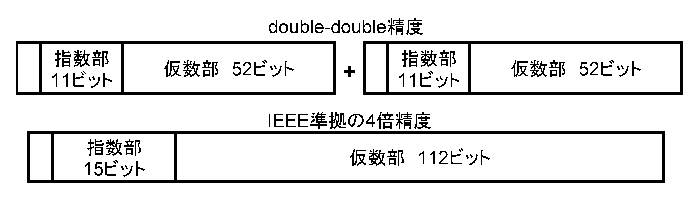
\includegraphics{double-double.eps}
\caption{double-double$B@:EY$N%S%C%H?t(B}
\label{fig:residual}
  }
\end{figure}


\subsection{4$BG\@:EY1i;;$NMxMQ(B}
\label{sec:testprog4}
Toepliz$B9TNs(B
\[
A = \left(
\begin{array}{cccccc}
2 & 1 &   &  &  & \\
0 & 2 & 1 &  &  & \\
\gamma & 0& 2 & 1 &  & \\
 & \ddots & \ddots & \ddots & \ddots & \\
 &  &   \gamma &0 &       2   & 1 \\
 &  &  &   \gamma & 0& 2 \\
\end{array}
\right)
\]
$B$KBP$9$k@~7?J}Dx<07O(B$Ax=b$$B$r;XDj$5$l$?2rK!$G2r$-(B, $B2r$rI=<($9$k(B
$B%F%9%H%W%m%0%i%`$,(B\verb|test5.c|$B$G$"$k(B. 
$B1&JU%Y%/%H%k(B$b$$B$O2r(B$x$$B$,$9$Y$F(B$1$$B$H$J$k$h$&$K(B
$B5a$a$F$$$k(B. $n$$B$O9TNs(B$A$$B$N<!?t$G$"$k(B. 
\verb|test5|$B$K$*$$$F(B, 
\newpage
{\bf $BG\@:EY$N>l9g(B}\\
\verb+      >./test5 200 2.0 -f double+ \\
$B$^$?$O(B \\
\verb+      >./test5 200 2.0+ \\
$B$HF~NO$7$F<B9T$9$k$H(B, $B0J2<$N7k2L$,F@$i$l$k(B. 

\begin{verbatim}
n = 200, gamma = 2.000000
initial vector x = 0
precision : double
solver    : BiCG 2
precon    : none
storage   : CRS
lis_solve : LIS_MAXITER(code=4)

BiCG: number of iterations     = 1001 (double = 1001, quad = 0)
BiCG: elapsed time             = 2.044368e-02 sec.
BiCG:   preconditioner         = 4.768372e-06 sec.
BiCG:     matrix creation      = 4.768372e-06 sec.
BiCG:   linear solver          = 2.043891e-02 sec.
BiCG: relative residual 2-norm = 8.917591e+01
\end{verbatim}

{\bf 4$BG\@:EY$N>l9g(B}\\
\verb+      >./test5 200 2.0 -f quad+\\
$B$HF~NO$7$F<B9T$9$k$H(B, $B0J2<$N7k2L$,F@$i$l$k(B. 

\begin{verbatim}
n = 200, gamma = 2.000000
initial vector x = 0
precision : quad
solver    : BiCG 2
precon    : none
storage   : CRS
lis_solve : normal end

BiCG: number of iterations     = 230 (double = 230, quad = 0)
BiCG: elapsed time             = 2.267408e-02 sec.
BiCG:   preconditioner         = 4.549026e-04 sec.
BiCG:     matrix creation      = 5.006790e-06 sec.
BiCG:   linear solver          = 2.221918e-02 sec.
BiCG: relative residual 2-norm = 6.499145e-11
\end{verbatim}
%%%%%%%%%%%%%%%%%%%%%%%%%%%%%%%%%%%%%%%%%%%%%%%%%%%%%%%%%%%%%%
%%%%%%%%%%%%%%%%%%%%%%%%%%%%%%%%%%%%%%%%%%%%%%%%%%%%%%%%%%%%%%
\newpage
\section{$B9TNs3JG<7A<0(B}
\label{sec:storages}
$BK\@a$G$O(B, $B%i%$%V%i%j$G;HMQ$G$-$k9TNs$N3JG<7A<0$K$D$$$F=R$Y$k(B. 
$B9TNs$N9T(B($BNs(B)$BHV9f$O(B0$B$+$i;O$^$k$b$N$H$9$k(B. 
$n \times n$$B9TNs(B$A=(a_{ij})$$B$NHsNmMWAG?t$r(B$nnz$$B$H$9$k(B. 

%%%%%%%%%%%%%%%%%%%%%%%%%%%%%%%%%%%%%%%%%%%%%%%%%%%%%%%%%%%%%%%%%%
% Compressed Row Storage (CRS)
%%%%%%%%%%%%%%%%%%%%%%%%%%%%%%%%%%%%%%%%%%%%%%%%%%%%%%%%%%%%%%%%%%
\subsection{Compressed Row Storage (CRS)}
CRS$B7A<0$O(B3$B$D$NG[Ns(B({\ttfamily ptr,index,value})$B$K3JG<$9$k(B. 
\begin{itemize}
\item $BD9$5(B$nnz$$B$NG\@:EYG[Ns(B{\ttfamily value}$B$O9TNs(B$A$$B$NHsNmMWAG$NCM$r9TJ}8~$K1h$C$F3JG<$9$k(B. 
\item $BD9$5(B$nnz$$B$N@0?tG[Ns(B{\ttfamily index}$B$OG[Ns(B{\ttfamily value}$B$K3JG<$5$l$?HsNmMWAG$NNsHV9f$r3JG<$9$k(B. 
\item $BD9$5(B$n+1$$B$N@0?tG[Ns(B{\ttfamily ptr}$B$OG[Ns(B{\ttfamily value}$B$H(B{\ttfamily index}$B$N3F9T$N3+;O0LCV$r3JG<$9$k(B. 
\end{itemize}

\subsubsection{$B9TNs$N:n$jJ}(B ($BC`<!(B, OpenMP$BHG(B)}
$B9TNs(B$A$$B$N(BCRS$B7A<0$G$N3JG<J}K!$r?^(B\ref{fig:storage01}$B$K<($9(B. 
$B$3$N9TNs$r(BCRS$B7A<0$G:n@.$9$k>l9g(B, $B%W%m%0%i%`$O0J2<$N$h$&$K5-=R$9$k(B. 
\begin{figure}[h]
{\centering 
\begin{minipage}{0.3\textwidth}
\begin{flushright}
$ \label{eq:mata}
A = \left(
\begin{array}{cccc}
11 &    &    &    \\
21 & 22 &    &    \\
   & 32 & 33 &    \\
41 &    & 43 & 44 \\
\end{array}\right)
$
\end{flushright}
\end{minipage}
\begin{minipage}{0.6\textwidth}
\begin{flushleft}
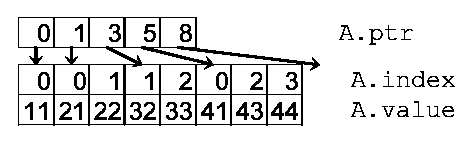
\includegraphics{storage01.eps} 
\end{flushleft}
\end{minipage}
\caption{CRS$B7A<0$N%G!<%?9=B$(B ($BC`<!(B, OpenMP$BHG(B)}\label{fig:storage01}}
\end{figure}
\begin{itembox}[l]{$BC`<!(B, OpenMP$BHG(B}
\small
\begin{verbatim}
 1: int           n,nnz;
 2: int           *ptr,*index;
 3: LIS_SCALAR    *value;
 4: LIS_MATRIX    A;
 5: n = 4; nnz = 8;
 6: ptr   = (int *)malloc( (n+1)*sizeof(int) );
 7: index = (int *)malloc( nnz*sizeof(int) );
 8: value = (LIS_SCALAR *)malloc( nnz*sizeof(LIS_SCALAR) );
 9: lis_matrix_create(0,&A);
10: lis_matrix_set_size(A,0,n);
11:
12: ptr[0] = 0; ptr[1] = 1; ptr[2] = 3; ptr[3] = 5; ptr[4] = 8;
13: index[0] =  0; index[1] =  0; index[2] =  1; index[3] =  1;
14: index[4] =  2; index[5] =  0; index[6] =  2; index[7] =  3;
15: value[0] = 11; value[1] = 21; value[2] = 22; value[3] = 32;
16: value[4] = 33; value[5] = 41; value[6] = 43; value[7] = 44;
17:
18:  lis_matrix_set_crs(nnz,ptr,index,value,A);
19:  lis_matrix_assemble(A);
\end{verbatim}
\end{itembox}
\subsubsection{$B9TNs$N:n$jJ}(B (MPI$BHG(B)}
2$B%W%m%;%9>e$X$N9TNs(B$A$$B$N(BCRS$B7A<0$G$N3JG<J}K!$r?^(B\ref{fig:storage01_mpi}$B$K<($9(B. 
2$B%W%m%;%9>e$K$3$N9TNs$r(BCRS$B7A<0$G:n@.$9$k>l9g(B, $B%W%m%0%i%`$O0J2<$N$h$&$K5-=R$9$k(B. 
\begin{figure}[h]
{\centering 
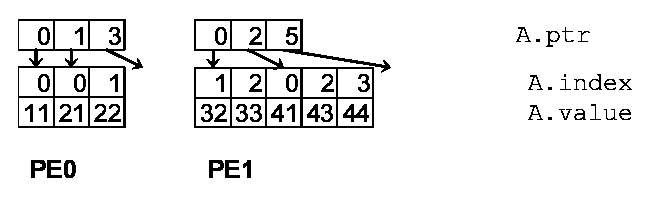
\includegraphics{storage01_mpi.eps} 
\caption{CRS$B7A<0$N%G!<%?9=B$(B (MPI$BHG(B)}\label{fig:storage01_mpi}}
\end{figure}
\begin{itembox}[l]{MPI$BHG(B}
\small
\begin{verbatim}
 1: int           i,k,n,nnz,my_rank;
 2: int           *ptr,*index;
 3: LIS_SCALAR    *value;
 4: LIS_MATRIX    A;
 5: MPI_Comm_rank(MPI_COMM_WORLD,&my_rank);
 6: if( my_rank==0 ) {n = 2; nnz = 3;}
 7: else             {n = 2; nnz = 5;}
 8: ptr   = (int *)malloc( (n+1)*sizeof(int) );
 9: index = (int *)malloc( nnz*sizeof(int) );
10: value = (LIS_SCALAR *)malloc( nnz*sizeof(LIS_SCALAR) );
11: lis_matrix_create(MPI_COMM_WORLD,&A);
12: lis_matrix_set_size(A,n,0);
13: if( my_rank==0 ) {
14:     ptr[0] = 0; ptr[1] = 1; ptr[2] = 3;
15:     index[0] =  0; index[1] =  0; index[2] =  1;
16:     value[0] = 11; value[1] = 21; value[2] = 22;}
17: else {
18:     ptr[0] = 0; ptr[1] = 2; ptr[2] = 5;
19:     index[0] =  1; index[1] =  2; index[2] =  0; index[3] =  2; index[4] =  3;
20:     value[0] = 32; value[1] = 33; value[2] = 41; value[3] = 43; value[4] = 44;}
21:  lis_matrix_set_crs(nnz,ptr,index,value,A);
22:  lis_matrix_assemble(A);
\end{verbatim}
\end{itembox}
\subsubsection{$B4XO"$9$k4X?t(B}
\noindent
{\bf $BG[Ns$N4XO"IU$1(B}

CRS$B7A<0$KI,MW$JG[Ns$r9TNs(B$A$$B$K4XO"IU$1$k$K$O4X?t(B

\begin{itemize}
\item \verb|C       int lis_matrix_set_crs(int nnz, int row[], int index[], LIS_SCALAR value[],|\\
      \verb| LIS_MATRIX A)|
\item \verb|Fortran subroutine lis_matrix_set_crs(integer nnz, integer row(), integer index(),|\\
      \verb| LIS_SCALAR value(), LIS_MATRIX A, integer ierr)|
\end{itemize}

$B$rMQ$$$k(B. 
%%%%%%%%%%%%%%%%%%%%%%%%%%%%%%%%%%%%%%%%%%%%%%%%%%%%%%%%%%%%%%%%%%
% Compressed Column Storage (CCS)
%%%%%%%%%%%%%%%%%%%%%%%%%%%%%%%%%%%%%%%%%%%%%%%%%%%%%%%%%%%%%%%%%%
\newpage
\subsection{Compressed Column Storage (CCS)}
CCS$B7A<0$O(B3$B$D$NG[Ns(B({\ttfamily ptr,index,value})$B$K3JG<$9$k(B. 
\begin{itemize}
\item $BD9$5(B$nnz$$B$NG\@:EYG[Ns(B{\ttfamily value}$B$O9TNs(B$A$$B$NHsNmMWAG$NCM$rNsJ}8~$K1h$C$F3JG<$9$k(B. 
\item $BD9$5(B$nnz$$B$N@0?tG[Ns(B{\ttfamily index}$B$OG[Ns(B{\ttfamily value}$B$K3JG<$5$l$?HsNmMWAG$N9THV9f$r3JG<$9$k(B. 
\item $BD9$5(B$n+1$$B$N@0?tG[Ns(B{\ttfamily ptr}$B$OG[Ns(B{\ttfamily value}$B$H(B{\ttfamily index}$B$N3FNs$N3+;O0LCV$r3JG<$9$k(B. 
\end{itemize}
\subsubsection{$B9TNs$N:n$jJ}(B ($BC`<!(B, OpenMP$BHG(B)}
$B9TNs(B$A$$B$N(BCCS$B7A<0$G$N3JG<J}K!$r?^(B\ref{fig:storage02}$B$K<($9(B. 
$B$3$N9TNs$r(BCCS$B7A<0$G:n@.$9$k>l9g(B, $B%W%m%0%i%`$O0J2<$N$h$&$K5-=R$9$k(B. 

\begin{figure}[h]
{\centering 
\begin{minipage}{0.3\textwidth}
\begin{flushright}
$ 
A = \left(
\begin{array}{cccc}
11 &    &    &    \\
21 & 22 &    &    \\
   & 32 & 33 &    \\
41 &    & 43 & 44 \\
\end{array}\right)
$
\end{flushright}
\end{minipage}
\begin{minipage}{0.6\textwidth}
\begin{flushleft}
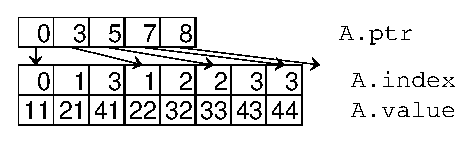
\includegraphics{storage02.eps} 
\end{flushleft}
\end{minipage}
\caption{CCS$B7A<0$N%G!<%?9=B$(B ($BC`<!(B, OpenMP$BHG(B)}\label{fig:storage02}}
\end{figure}
\begin{itembox}[l]{$BC`<!(B, OpenMP$BHG(B}
\small
\begin{verbatim}
 1: int           n,nnz;
 2: int           *ptr,*index;
 3: LIS_SCALAR    *value;
 4: LIS_MATRIX    A;
 5: n = 4; nnz = 8;
 6: ptr   = (int *)malloc( (n+1)*sizeof(int) );
 7: index = (int *)malloc( nnz*sizeof(int) );
 8: value = (LIS_SCALAR *)malloc( nnz*sizeof(LIS_SCALAR) );
 9: lis_matrix_create(0,&A);
10: lis_matrix_set_size(A,0,n);
11:
12: ptr[0] = 0; ptr[1] = 3; ptr[2] = 5; ptr[3] = 7; ptr[4] = 8;
13: index[0] =  0; index[1] =  1; index[2] =  3; index[3] =  1;
14: index[4] =  2; index[5] =  2; index[6] =  3; index[7] =  3;
15: value[0] = 11; value[1] = 21; value[2] = 41; value[3] = 22;
16: value[4] = 32; value[5] = 33; value[6] = 43; value[7] = 44;
17:
18:  lis_matrix_set_ccs(nnz,ptr,index,value,A);
19:  lis_matrix_assemble(A);
\end{verbatim}
\end{itembox}
\newpage
\subsubsection{$B9TNs$N:n$jJ}(B (MPI$BHG(B)}
2$B%W%m%;%9>e$X$N9TNs(B$A$$B$N(BCCS$B7A<0$G$N3JG<J}K!$r?^(B\ref{fig:storage02_mpi}$B$K(B
$B<($9(B. 
2$B%W%m%;%9>e$K$3$N9TNs$r(BCCS$B7A<0$G:n@.$9$k>l9g(B, $B%W%m%0%i%`$O0J2<$N$h$&$K5-=R$9$k(B. 
\begin{figure}[h]
{\centering 
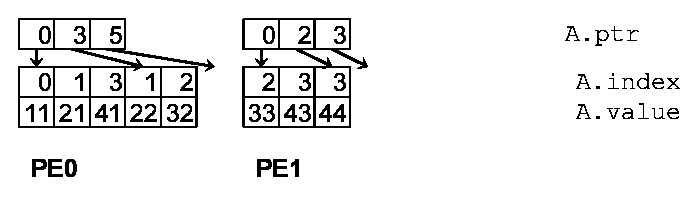
\includegraphics{storage02_mpi.eps} 
\caption{CCS$B7A<0$N%G!<%?9=B$(B (MPI$BHG(B)}\label{fig:storage02_mpi}}
\end{figure}
\begin{itembox}[l]{MPI$BHG(B}
\small
\begin{verbatim}
 1: int           i,k,n,nnz,my_rank;
 2: int           *ptr,*index;
 3: LIS_SCALAR    *value;
 4: LIS_MATRIX    A;
 5: MPI_Comm_rank(MPI_COMM_WORLD,&my_rank);
 6: if( my_rank==0 ) {n = 2; nnz = 3;}
 7: else             {n = 2; nnz = 5;}
 8: ptr   = (int *)malloc( (n+1)*sizeof(int) );
 9: index = (int *)malloc( nnz*sizeof(int) );
10: value = (LIS_SCALAR *)malloc( nnz*sizeof(LIS_SCALAR) );
11: lis_matrix_create(MPI_COMM_WORLD,&A);
12: lis_matrix_set_size(A,n,0);
13: if( my_rank==0 ) {
14:     ptr[0] = 0; ptr[1] = 3; ptr[2] = 5;
15:     index[0] =  0; index[1] =  1; index[2] =  3; index[3] =  1; index[4] =  2;
16:     value[0] = 11; value[1] = 21; value[2] = 41; value[3] = 22; value[4] = 32}
17: else {
18:     ptr[0] = 0; ptr[1] = 2; ptr[2] = 3;
19:     index[0] =  2; index[1] =  3; index[2] =  3;
20:     value[0] = 33; value[1] = 43; value[2] = 44;}
21:  lis_matrix_set_ccs(nnz,ptr,index,value,A);
22:  lis_matrix_assemble(A);
\end{verbatim}
\end{itembox}
\subsubsection{$B4XO"$9$k4X?t(B}
\noindent
{\bf $BG[Ns$N4XO"IU$1(B}

CCS$B7A<0$KI,MW$JG[Ns$r9TNs(B$A$$B$K4XO"IU$1$k$K$O4X?t(B
\begin{itemize}
\item \verb|C       int lis_matrix_set_ccs(int nnz, int row[], int index[], LIS_SCALAR value[],|\\
      \verb| LIS_MATRIX A)|
\item \verb|Fortran subroutine lis_matrix_set_ccs(integer nnz, integer row(), integer index(),|\\
      \verb| LIS_SCALAR value(), LIS_MATRIX A, integer ierr)|
\end{itemize}
$B$rMQ$$$k(B. 

%%%%%%%%%%%%%%%%%%%%%%%%%%%%%%%%%%%%%%%%%%%%%%%%%%%%%%%%%%%%%%%%%%
% Modified Compressed Sparse Row (MSR)
%%%%%%%%%%%%%%%%%%%%%%%%%%%%%%%%%%%%%%%%%%%%%%%%%%%%%%%%%%%%%%%%%%
\newpage
\subsection{Modified Compressed Sparse Row (MSR)}
MSR$B7A<0$O(BCRS$B7A<0$r=$@5$7$?$b$N$G$"$k(B. $B$=$N0c$$$OBP3QItJ,$rJ,$1$F3JG<$7$F$$$k$H$3$m$G$"$k(B. 
MSR$B7A<0$O(B2$B$D$NG[Ns(B({\ttfamily index,value})$B$K3JG<$9$k(B. $ndz$$B$rBP3QItJ,$NNmMWAG?t$H$9$k(B. 
\begin{itemize}
\item $BD9$5(B$nnz + ndz + 1$$B$NG\@:EYG[Ns(B{\ttfamily value}$B$O(B
$n$$BHVL\$^$G$O9TNs(B$A$$B$NBP3QItJ,$r3JG<$9$k(B. $n+1$$BHVL\$NMWAG$O;HMQ$7$J$$(B. $n+2$$BHVL\$+$i$O(B
$B9TNs(B$A$$B$NBP3Q0J30$NHsNmMWAG$NCM$r9TJ}8~$K1h$C$F3JG<$9$k(B. 
\item $BD9$5(B$nnz + ndz + 1$$B$N@0?tG[Ns(B{\ttfamily index}$B$O(B
$n+1$$BHVL\$^$G$O9TNs(B$A$$B$NHsBP3QItJ,$N3F9T$N3+;O0LCV$r3JG<$9$k(B. 
$n+2$$BHVL\$+$i$O9TNs(B$A$$B$NHsBP3QItJ,$NG[Ns(B{\ttfamily value}$B$K3JG<$5$l$?HsNmMWAG$NNsHV9f$r3JG<$9$k(B. 
\end{itemize}
\subsubsection{$B9TNs$N:n$jJ}(B ($BC`<!(B, OpenMP$BHG(B)}
$B9TNs(B$A$$B$N(BMSR$B7A<0$G$N3JG<J}K!$r?^(B\ref{fig:storage03}$B$K<($9(B. 
$B$3$N9TNs$r(BMSR$B7A<0$G:n@.$9$k>l9g(B, $B%W%m%0%i%`$O0J2<$N$h$&$K5-=R$9$k(B. 

\begin{figure}[h]
{\centering 
\begin{minipage}{0.3\textwidth}
\begin{flushright}
$ 
A = \left(
\begin{array}{cccc}
11 &    &    &    \\
21 & 22 &    &    \\
   & 32 & 33 &    \\
41 &    & 43 & 44 \\
\end{array}\right)
$
\end{flushright}
\end{minipage}
\begin{minipage}{0.6\textwidth}
\begin{flushleft}
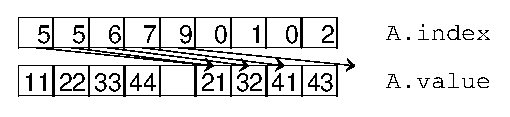
\includegraphics{storage03.eps} 
\end{flushleft}
\end{minipage}
\caption{MSR$B7A<0$N%G!<%?9=B$(B ($BC`<!(B, OpenMP$BHG(B)}\label{fig:storage03}}
\end{figure}
\begin{itembox}[l]{$BC`<!(B, OpenMP$BHG(B}
\small
\begin{verbatim}
 1: int           n,nnz,ndz;
 2: int           *index;
 3: LIS_SCALAR    *value;
 4: LIS_MATRIX    A;
 5: n = 4; nnz = 8; ndz = 0;
 6: index = (int *)malloc( (nnz+ndz+1)*sizeof(int) );
 7: value = (LIS_SCALAR *)malloc( (nnz+ndz+1)*sizeof(LIS_SCALAR) );
 8: lis_matrix_create(0,&A);
 9: lis_matrix_set_size(A,0,n);
10:
11: index[0] =  5; index[1] =  5; index[2] =  6; index[3] =  7;
12: index[4] =  9; index[5] =  0; index[6] =  1; index[7] =  0; index[8] =  2;
13: value[0] = 11; value[1] = 22; value[2] = 33; value[3] = 44;
14: value[4] =  0; value[5] = 21; value[6] = 32; value[7] = 41; value[8] = 43;
15:
16:  lis_matrix_set_msr(nnz,ndz,index,value,A);
17:  lis_matrix_assemble(A);
\end{verbatim}
\end{itembox}
\newpage
\subsubsection{$B9TNs$N:n$jJ}(B (MPI$BHG(B)}
2$B%W%m%;%9>e$X$N9TNs(B$A$$B$N(BMSR$B7A<0$G$N3JG<J}K!$r?^(B\ref{fig:storage03_mpi}$B$K(B
$B<($9(B. 
2$B%W%m%;%9>e$K$3$N9TNs$r(BMSR$B7A<0$G:n@.$9$k>l9g(B, $B%W%m%0%i%`$O0J2<$N$h$&$K5-=R$9$k(B. 
\begin{figure}[h]
{\centering 
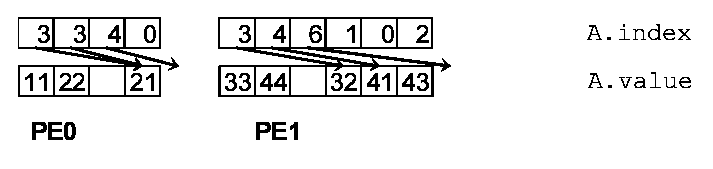
\includegraphics{storage03_mpi.eps} 
\caption{MSR$B7A<0$N%G!<%?9=B$(B (MPI$BHG(B)}\label{fig:storage03_mpi}}
\end{figure}
\begin{itembox}[l]{MPI$BHG(B}
\small
\begin{verbatim}
 1: int           i,k,n,nnz,ndz,my_rank;
 2: int           *index;
 3: LIS_SCALAR    *value;
 4: LIS_MATRIX    A;
 5: MPI_Comm_rank(MPI_COMM_WORLD,&my_rank);
 6: if( my_rank==0 ) {n = 2; nnz = 3; ndz = 0;}
 7: else             {n = 2; nnz = 5; ndz = 0;}
 8: index = (int *)malloc( (nnz+ndz+1)*sizeof(int) );
 9: value = (LIS_SCALAR *)malloc( (nnz+ndz+1)*sizeof(LIS_SCALAR) );
10: lis_matrix_create(MPI_COMM_WORLD,&A);
11: lis_matrix_set_size(A,n,0);
12: if( my_rank==0 ) {
13:     index[0] =  3; index[1] =  3; index[2] =  4; index[3] =  0;
14:     value[0] = 11; value[1] = 22; value[2] =  0; value[3] = 21;}
15: else {
16:     index[0] =  3; index[1] =  4; index[2] =  6; index[3] =  1;
17:     index[4] =  0; index[5] =  2;
18:     value[0] = 33; value[1] = 44; value[2] =  0; value[3] = 32;
19:     value[4] = 41; value[5] = 43;}
20:  lis_matrix_set_msr(nnz,ndz,index,value,A);
21:  lis_matrix_assemble(A);
\end{verbatim}
\end{itembox}
\subsubsection{$B4XO"$9$k4X?t(B}
\noindent
{\bf $BG[Ns$N4XO"IU$1(B}

MSR$B7A<0$KI,MW$JG[Ns$r9TNs(B$A$$B$K4XO"IU$1$k$K$O4X?t(B
\begin{itemize}
\item \verb|C       int lis_matrix_set_msr(int nnz, int ndz, int index[], LIS_SCALAR value[], |\\
      \verb|LIS_MATRIX A)|
\item \verb|Fortran subroutine lis_matrix_set_msr(integer nnz, integer ndz, integer index(),|\\
      \verb| LIS_SCALAR value(), LIS_MATRIX A, integer ierr)|
\end{itemize}
$B$rMQ$$$k(B. 

%%%%%%%%%%%%%%%%%%%%%%%%%%%%%%%%%%%%%%%%%%%%%%%%%%%%%%%%%%%%%%%%%%
% Diagonal (DIA)
%%%%%%%%%%%%%%%%%%%%%%%%%%%%%%%%%%%%%%%%%%%%%%%%%%%%%%%%%%%%%%%%%%
\newpage
\subsection{Diagonal (DIA)}
DIA$B$O(B2$B$D$NG[Ns(B({\ttfamily index, value})$B$K3JG<$9$k(B. 
$nnd$$B$r9TNs(B$A$$B$NHsNm$JBP3QMWAG$NK\?t$H$9$k(B. 
\begin{itemize}
\item $BD9$5(B$nnd \times n$$B$NG\@:EYG[Ns(B{\ttfamily value}$B$O9TNs(B$A$$B$NHsNm$JBP(B
      $B3QMWAG$r3JG<$9$k(B. 
\item $BD9$5(B$nnd$$B$N@0?tG[Ns(B{\ttfamily index}$B$O<gBP3QMWAG$+$i3FBP3QMWAG$X$N%*%U%;%C%H$r3JG<$9$k(B. 
\end{itemize}
OpenMP$BHG$G$O0J2<$N$h$&$K=$@5$7$F$$$k(B. \\
DIA$B$O(B2$B$D$NG[Ns(B({\ttfamily index, value})$B$K3JG<$9$k(B. $nprocs$$B$r%9%l%C%I?t$H$9$k(B. 
$nnd_p$$B$r9TNs(B$A$$B$r9T%V%m%C%/J,3d$7$?ItJ,9TNs$NHsNm$JBP3Q$NK\?t$H$9$k(B. 
$maxnnd$$B$r(B$nnd_p$$B$NCM$N:GBgCM$H$9$k(B. 
\begin{itemize}
\item $BD9$5(B$maxnnd \times n$$B$NG\@:EYG[Ns(B{\ttfamily value}$B$O9TNs(B$A$$B$r9T%V(B
      $B%m%C%/J,3d$7$?ItJ,9TNs$NHsNm$JBP3QMWAG$r3JG<$9$k(B. 
\item $BD9$5(B$nprocs \times maxnnd$$B$N@0?tG[Ns(B{\ttfamily index}$B$O<gBP3QMWAG$+$i3FBP3QMWAG$X$N%*%U%;%C%H$r3JG<$9$k(B. 
\end{itemize}
\subsubsection{$B9TNs$N:n$jJ}(B ($BC`<!HG(B)}
$B9TNs(B$A$$B$N(BDIA$B7A<0$G$N3JG<J}K!$r?^(B\ref{fig:storage04}$B$K<($9(B. 
$B$3$N9TNs$r(BDIA$B7A<0$G:n@.$9$k>l9g(B, $B%W%m%0%i%`$O0J2<$N$h$&$K5-=R$9$k(B. 
\begin{figure}[h]
{\centering 
\begin{minipage}{0.3\textwidth}
\begin{flushright}
$ 
A = \left(
\begin{array}{cccc}
11 &    &    &    \\
21 & 22 &    &    \\
   & 32 & 33 &    \\
41 &    & 43 & 44 \\
\end{array}\right)
$
\end{flushright}
\end{minipage}
\begin{minipage}{0.6\textwidth}
\begin{flushleft}
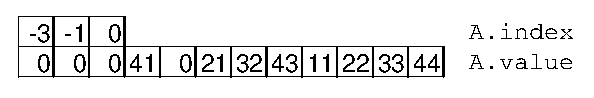
\includegraphics{storage04.eps} 
\end{flushleft}
\end{minipage}
\caption{DIA$B7A<0$N%G!<%?9=B$(B ($BC`<!HG(B)}\label{fig:storage04}}
\end{figure}
\begin{itembox}[l]{$BC`<!HG(B}
\small
\begin{verbatim}
 1: int           n,nnd;
 2: int           *index;
 3: LIS_SCALAR    *value;
 4: LIS_MATRIX    A;
 5: n = 4; nnd = 3;
 6: index = (int *)malloc( nnd*sizeof(int) );
 7: value = (LIS_SCALAR *)malloc( n*nnd*sizeof(LIS_SCALAR) );
 8: lis_matrix_create(0,&A);
 9: lis_matrix_set_size(A,0,n);
10:
11: index[0] = -3; index[1] = -1; index[2] =  0;
12: value[0] =  0; value[1] =  0; value[2] =  0; value[3] = 41;
13: value[4] =  0; value[5] = 21; value[6] = 32; value[7] = 43;
14: value[8] = 11; value[9] = 22; value[10]= 33; value[11]= 44;
15:
16:  lis_matrix_set_dia(nnd,index,value,A);
17:  lis_matrix_assemble(A);
\end{verbatim}
\end{itembox}
\subsubsection{$B9TNs$N:n$jJ}(B (OpenMP$BHG(B)}
2$B%9%l%C%I>e$X$N9TNs(B$A$$B$N(BDIA$B7A<0$G$N3JG<J}K!$r?^(B\ref{fig:storage04_omp}$B$K(B
$B<($9(B. 
2$B%9%l%C%I>e$K$3$N9TNs$r(BDIA$B7A<0$G:n@.$9$k>l9g(B, $B%W%m%0%i%`$O0J2<$N$h$&$K5-=R$9$k(B. 
\begin{figure}[h]
{\centering 
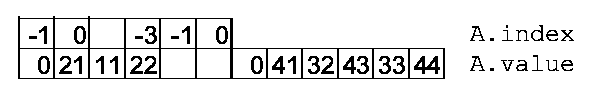
\includegraphics{storage04_omp.eps} 
\caption{DIA$B7A<0$N%G!<%?9=B$(B (OpenMP$BHG(B)}\label{fig:storage04_omp}}
\end{figure}
\begin{itembox}[l]{OpenMP$BHG(B}
\small
\begin{verbatim}
 1: int           n,maxnnd,nprocs;
 2: int           *index;
 3: LIS_SCALAR    *value;
 4: LIS_MATRIX    A;
 5: n = 4; maxnnd = 3; nprocs = 2;
 6: index = (int *)malloc( maxnnd*sizeof(int) );
 7: value = (LIS_SCALAR *)malloc( n*maxnnd*sizeof(LIS_SCALAR) );
 8: lis_matrix_create(0,&A);
 9: lis_matrix_set_size(A,0,n);
10:
11: index[0] = -1; index[1] =  0; index[2] =  0; index[3] = -3; index[4] = -1; index[5] =  0;
12: value[0] =  0; value[1] = 21; value[2] = 11; value[3] = 22; value[4] =  0; value[5] =  0;
13: value[6] =  0; value[7] = 41; value[8] = 32; value[9] = 43; value[10]= 33; value[11]= 44;
14:
15:  lis_matrix_set_dia(maxnnd,index,value,A);
16:  lis_matrix_assemble(A);
\end{verbatim}
\end{itembox}
\newpage
\subsubsection{$B9TNs$N:n$jJ}(B (MPI$BHG(B)}
2$B%W%m%;%9>e$X$N9TNs(B$A$$B$N(BDIA$B7A<0$G$N3JG<J}K!$r?^(B\ref{fig:storage04_mpi}$B$K(B
$B<($9(B. 
2$B%W%m%;%9>e$K$3$N9TNs$r(BDIA$B7A<0$G:n@.$9$k>l9g(B, $B%W%m%0%i%`$O0J2<$N$h$&$K5-=R$9$k(B. 
\begin{figure}[h]
{\centering 
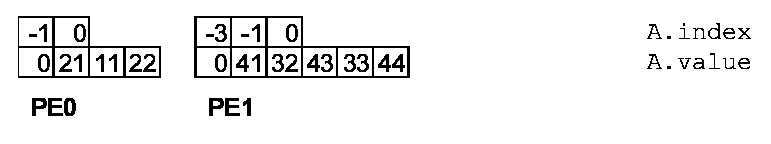
\includegraphics{storage04_mpi.eps} 
\caption{DIA$B7A<0$N%G!<%?9=B$(B (MPI$BHG(B)}\label{fig:storage04_mpi}}
\end{figure}
\begin{itembox}[l]{MPI$BHG(B}
\small
\begin{verbatim}
 1: int           i,n,nnd,my_rank;
 2: int           *index;
 3: LIS_SCALAR    *value;
 4: LIS_MATRIX    A;
 5: MPI_Comm_rank(MPI_COMM_WORLD,&my_rank);
 6: if( my_rank==0 ) {n = 2; nnd = 2;}
 7: else             {n = 2; nnd = 3;}
 8: index = (int *)malloc( nnd*sizeof(int) );
 9: value = (LIS_SCALAR *)malloc( n*nnd*sizeof(LIS_SCALAR) );
10: lis_matrix_create(MPI_COMM_WORLD,&A);
11: lis_matrix_set_size(A,n,0);
12: if( my_rank==0 ) {
13:     index[0] = -1; index[1] =  0;
14:     value[0] =  0; value[1] = 21; value[2] = 11; value[3] = 22;}
15: else {
16:     index[0] = -3; index[1] = -1; index[2] =  0;
17:     value[0] =  0; value[1] = 41; value[2] = 32; value[3] = 43; value[4] = 33;
18:     value[5] = 44;}
19:  lis_matrix_set_dia(nnd,index,value,A);
20:  lis_matrix_assemble(A);
\end{verbatim}
\end{itembox}
\subsubsection{$B4XO"$9$k4X?t(B}
\noindent
{\bf $BG[Ns$N4XO"IU$1(B}

DIA$B7A<0$KI,MW$JG[Ns$r9TNs(B$A$$B$K4XO"IU$1$k$K$O4X?t(B
\begin{itemize}
\item \verb|C       int lis_matrix_set_dia(int nnd, int index[], LIS_SCALAR value[], LIS_MATRIX A)|
\item \verb|Fortran subroutine lis_matrix_set_dia(integer nnd, integer index(), LIS_SCALAR value(),|\\
      \verb| LIS_MATRIX A, integer ierr)|
\end{itemize}
$B$rMQ$$$k(B. 

%%%%%%%%%%%%%%%%%%%%%%%%%%%%%%%%%%%%%%%%%%%%%%%%%%%%%%%%%%%%%%%%%%
% Ellpack-Itpack generalized diagonal (ELL)
%%%%%%%%%%%%%%%%%%%%%%%%%%%%%%%%%%%%%%%%%%%%%%%%%%%%%%%%%%%%%%%%%%
\newpage
\subsection{Ellpack-Itpack generalized diagonal (ELL)}
ELL$B$O(B2$B$D$NG[Ns(B({\ttfamily index, value})$B$K3JG<$9$k(B. 
$maxnzr$$B$r9TNs(B$A$$B$N3F9T$G$NHsNmMWAG?t$N:GBgCM$H$9$k(B. 
\begin{itemize}
\item $BD9$5(B$maxnzr \times n$$B$NG\@:EYG[Ns(B{\ttfamily value}$B$O9TNs(B$A$$B$N3F9T$NHsNmMWAG$rNsJ}8~$K1h$C$F3JG<$9$k(B. 
$B:G=i$NNs$O3F9T$N:G=i$NHsNmMWAG$+$i$J$k(B. $B$?$@$7(B, $B3JG<$9$kHsNmMWAG$,$J$$>l9g$O(B$0$$B$r3JG<$9$k(B. 
\item $BD9$5(B$maxnzr \times n$$B$N@0?tG[Ns(B{\ttfamily index}$B$O(B
$BG[Ns(B{\ttfamily value}$B$K3JG<$5$l$?HsNmMWAG$NNsHV9f$r3JG<$9$k(B. 
$B$?$@$7(B, $BBh(B$i$$B9TL\$NHsNmMWAG?t$r(B$nnz$$B$H$9$k$H(B{\tt index[$nnz \times + i$]}$B$K$O$=$N9THV9f(B$i$$B$r3JG<$9$k(B. 
\end{itemize}
\subsubsection{$B9TNs$N:n$jJ}(B ($BC`<!(B, OpenMP$BHG(B)}
$B9TNs(B$A$$B$N(BELL$B7A<0$G$N3JG<J}K!$r?^(B\ref{fig:storage05}$B$K<($9(B. 
$B$3$N9TNs$r(BELL$B7A<0$G:n@.$9$k>l9g(B, $B%W%m%0%i%`$O0J2<$N$h$&$K5-=R$9$k(B. 
\begin{figure}[h]
{\centering 
\begin{minipage}{0.3\textwidth}
\begin{flushright}
$ 
A = \left(
\begin{array}{cccc}
11 &    &    &    \\
21 & 22 &    &    \\
   & 32 & 33 &    \\
41 &    & 43 & 44 \\
\end{array}\right)
$
\end{flushright}
\end{minipage}
\begin{minipage}{0.6\textwidth}
\begin{flushleft}
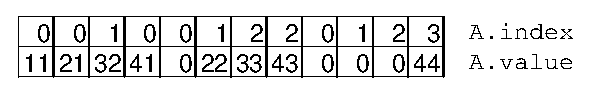
\includegraphics{storage05.eps} 
\end{flushleft}
\end{minipage}
\caption{ELL$B7A<0$N%G!<%?9=B$(B ($BC`<!(B, OpenMP$BHG(B)}\label{fig:storage05}}
\end{figure}
\begin{itembox}[l]{$BC`<!(B, OpenMP$BHG(B}
\small
\begin{verbatim}
 1: int           n,maxnzr;
 2: int           *index;
 3: LIS_SCALAR    *value;
 4: LIS_MATRIX    A;
 5: n = 4; maxnzr = 3;
 6: index = (int *)malloc( n*maxnzr*sizeof(int) );
 7: value = (LIS_SCALAR *)malloc( n*maxnzr*sizeof(LIS_SCALAR) );
 8: lis_matrix_create(0,&A);
 9: lis_matrix_set_size(A,0,n);
10:
11: index[0] =  0; index[1] =  0; index[2] =  1; index[3] =  0; index[4] =  0; index[5] =  1;
12: index[6] =  2; index[7] =  2; index[8] =  0; index[9] =  1; index[10]=  2; index[11]=  3;
13: value[0] = 11; value[1] = 21; value[2] = 32; value[3] = 41; value[4] =  0; value[5] = 22;
14: value[6] = 33; value[7] = 43; value[8] =  0; value[9] =  0; value[10]=  0; value[11]= 44;
15:
16:  lis_matrix_set_ell(maxnzr,index,value,A);
17:  lis_matrix_assemble(A);
\end{verbatim}
\end{itembox}
\newpage
\subsubsection{$B9TNs$N:n$jJ}(B (MPI$BHG(B)}
2$B%W%m%;%9>e$X$N9TNs(B$A$$B$N(BELL$B7A<0$G$N3JG<J}K!$r?^(B\ref{fig:storage05_mpi}$B$K(B
$B<($9(B. 
2$B%W%m%;%9>e$K$3$N9TNs$r(BELL$B7A<0$G:n@.$9$k>l9g(B, $B%W%m%0%i%`$O0J2<$N$h$&$K5-=R$9$k(B. 
\begin{figure}[h]
{\centering 
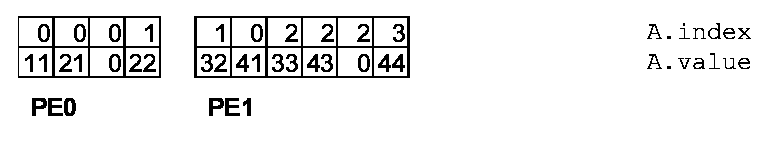
\includegraphics{storage05_mpi.eps} 
\caption{ELL$B7A<0$N%G!<%?9=B$(B (MPI$BHG(B)}\label{fig:storage05_mpi}}
\end{figure}
\begin{itembox}[l]{MPI$BHG(B}
\small
\begin{verbatim}
 1: int           i,n,maxnzr,my_rank;
 2: int           *index;
 3: LIS_SCALAR    *value;
 4: LIS_MATRIX    A;
 5: MPI_Comm_rank(MPI_COMM_WORLD,&my_rank);
 6: if( my_rank==0 ) {n = 2; maxnzr = 2;}
 7: else             {n = 2; maxnzr = 3;}
 8: index = (int *)malloc( n*maxnzr*sizeof(int) );
 9: value = (LIS_SCALAR *)malloc( n*maxnzr*sizeof(LIS_SCALAR) );
10: lis_matrix_create(MPI_COMM_WORLD,&A);
11: lis_matrix_set_size(A,n,0);
12: if( my_rank==0 ) {
13:     index[0] =  0; index[1] =  0; index[2] =  0; index[3] =  1;
14:     value[0] = 11; value[1] = 21; value[2] =  0; value[3] = 22;}
15: else {
16:     index[0] =  1; index[1] =  0; index[2] =  2; index[3] =  2; index[4] =  2;
17:     index[5] =  3;
18:     value[0] = 32; value[1] = 41; value[2] = 33; value[3] = 43; value[4] =  0;
19:     value[5] = 44;}
20:  lis_matrix_set_ell(maxnzr,index,value,A);
21:  lis_matrix_assemble(A);
\end{verbatim}
\end{itembox}
\subsubsection{$B4XO"$9$k4X?t(B}
\noindent
{\bf $BG[Ns$N4XO"IU$1(B}

ELL$B7A<0$KI,MW$JG[Ns$r9TNs(B$A$$B$K4XO"IU$1$k$K$O4X?t(B
\begin{itemize}
\item \verb|C       int lis_matrix_set_ell(int maxnzr, int index[], LIS_SCALAR value[],|\\
      \verb| LIS_MATRIX A)|
\item \verb|Fortran subroutine lis_matrix_set_ell(integer maxnzr, integer index(),|\\
      \verb| LIS_SCALAR value(), LIS_MATRIX A, integer ierr)|
\end{itemize}
$B$rMQ$$$k(B. 

%%%%%%%%%%%%%%%%%%%%%%%%%%%%%%%%%%%%%%%%%%%%%%%%%%%%%%%%%%%%%%%%%%
% Jagged Diagonal (JDS)
%%%%%%%%%%%%%%%%%%%%%%%%%%%%%%%%%%%%%%%%%%%%%%%%%%%%%%%%%%%%%%%%%%
\newpage
\subsection{Jagged Diagonal (JDS)}
JDS$B$O:G=i$K3F9T$NHsNmMWAG?t$NBg$-$$=g$K9T$NJB$SBX$($r9T$$(B, 
$B3F9T$NHsNmMWAG$rNsJ}8~$K1h$C$F3JG<$9$k(B. 
JDS$B$O(B4$B$D$NG[Ns(B({\ttfamily perm, ptr, index, value})$B$K3JG<$9$k(B. 
$maxnzr$$B$r9TNs(B$A$$B$N3F9T$G$NHsNmMWAG?t$N:GBgCM$H$9$k(B. 
\begin{itemize}
\item $BD9$5(B$n$$B$N@0?tG[Ns(B{\ttfamily perm}$B$OJB$SBX$($?9THV9f$r3JG<$9$k(B. 
\item $BD9$5(B$nnz$$B$NG\@:EYG[Ns(B{\ttfamily value}$B$OJB$SBX$($i$l$?9TNs(B$A$$B$N5x(B
      $B;u>uBP3QMWAG$r3JG<$9$k(B. 
$B:G=i$N5x;u>uBP3QMWAG$O3F9T$N:G=i$NHsNmMWAG$+$i$J$k(B. 
$B<!$N5x;u>uBP3QMWAG$O3F9T$N#2HVL\$NHsNmMWAG$+$i$J$k(B. $B$3$l$r=g<!7+$jJV$7$F$$$/(B. 
\item $BD9$5(B$nnz$$B$N@0?tG[Ns(B{\ttfamily index}$B$OG[Ns(B{\ttfamily value}$B$K3JG<$5$l$?HsNmMWAG$NNsHV9f$r3JG<$9$k(B. 
\item $BD9$5(B$maxnzr + 1$$B$N@0?tG[Ns(B{\ttfamily ptr}$B$O3F5x;u>uBP3QMWAG$N3+;O0LCV$r3JG<$9$k(B. 
\end{itemize}
OpenMP$BHG$G$O0J2<$N$h$&$K=$@5$r9T$C$F$$$k(B. \\
JDS$B$O(B4$B$D$NG[Ns(B({\ttfamily perm, ptr, index, value})$B$K3JG<$9$k(B. 
$nprocs$$B$r%9%l%C%I?t$H$9$k(B. 
$maxnzr_p$$B$r9TNs(B$A$$B$r9T%V%m%C%/J,3d$7$?ItJ,9TNs$N3F9T$G$NHsNmMWAG?t$N:GBgCM$H$9$k(B. 
$maxmaxnzr$$B$OG[Ns(B$maxnzr_p$$B$NCM$N:GBgCM$G$"$k(B. 
\begin{itemize}
\item $BD9$5(B$n$$B$N@0?tG[Ns(B{\ttfamily perm}$B$O9TNs(B$A$$B$r9T%V%m%C%/J,3d$7$?ItJ,9TNs$rJB$SBX$($?9THV9f$r3JG<$9$k(B. 
\item $BD9$5(B$nnz$$B$NG\@:EYG[Ns(B{\ttfamily value}$B$OJB$SBX$($i$l$?9TNs(B$A$$B$N5x(B
      $B;u>uBP3QMWAG$r3JG<$9$k(B. 
$B:G=i$N5x;u>uBP3QMWAG$O3F9T$N:G=i$NHsNmMWAG$+$i$J$k(B. 
$B<!$N5x;u>uBP3QMWAG$O3F9T$N#2HVL\$NHsNmMWAG$+$i$J$k(B. $B$3$l$r=g<!7+$jJV$7$F$$$/(B. 
\item $BD9$5(B$nnz$$B$N@0?tG[Ns(B{\ttfamily index}$B$OG[Ns(B{\ttfamily value}$B$K3JG<$5$l$?HsNmMWAG$NNsHV9f$r3JG<$9$k(B. 
\item $BD9$5(B$nprocs \times (maxmaxnzr + 1)$$B$N@0?tG[Ns(B{\ttfamily ptr}$B$O9TNs(B
      $A$$B$r9T%V%m%C%/J,3d$7$?ItJ,9TNs$N3F5x;u>uBP3QMWAG$N3+;O0LCV$r3JG<$9$k(B. 
\end{itemize}
\newpage
\subsubsection{$B9TNs$N:n$jJ}(B ($BC`<!HG(B)}
$B9TNs(B$A$$B$N(BJDS$B7A<0$G$N3JG<J}K!$r?^(B\ref{fig:storage06}$B$K<($9(B. 
$B$3$N9TNs$r(BJDS$B7A<0$G:n@.$9$k>l9g(B, $B%W%m%0%i%`$O0J2<$N$h$&$K5-=R$9$k(B. 
\begin{figure}[h]
{\centering 
\begin{minipage}{0.3\textwidth}
\begin{flushright}
$ 
A = \left(
\begin{array}{cccc}
11 &    &    &    \\
21 & 22 &    &    \\
   & 32 & 33 &    \\
41 &    & 43 & 44 \\
\end{array}\right)
$
\end{flushright}
\end{minipage}
\begin{minipage}{0.6\textwidth}
\begin{flushleft}
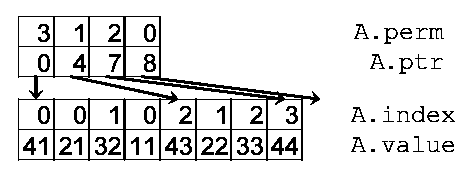
\includegraphics{storage06.eps} 
\end{flushleft}
\end{minipage}
\caption{JDS$B7A<0$N%G!<%?9=B$(B ($BC`<!HG(B)}\label{fig:storage06}}
\end{figure}
\begin{itembox}[l]{$BC`<!HG(B}
\small
\begin{verbatim}
 1: int           n,nnz,maxnzr;
 2: int           *perm,*ptr,*index;
 3: LIS_SCALAR    *value;
 4: LIS_MATRIX    A;
 5: n = 4; nnz = 8; maxnzr = 3;
 6: perm  = (int *)malloc( n*sizeof(int) );
 7: ptr   = (int *)malloc( (maxnzr+1)*sizeof(int) );
 8: index = (int *)malloc( nnz*sizeof(int) );
 9: value = (LIS_SCALAR *)malloc( nnz*sizeof(LIS_SCALAR) );
10: lis_matrix_create(0,&A);
11: lis_matrix_set_size(A,0,n);
12:
13: perm[0] = 3; perm[1] = 1; perm[2] = 2; perm[3] = 0;
14: ptr[0]  = 0; ptr[1]  = 4; ptr[2]  = 7; ptr[3]  = 8;
15: index[0] =  0; index[1] =  0; index[2] =  1; index[3] =  0;
16: index[4] =  2; index[5] =  1; index[6] =  2; index[7] =  3;
17: value[0] = 41; value[1] = 21; value[2] = 32; value[3] = 11;
18: value[4] = 43; value[5] = 22; value[6] = 33; value[7] = 44;
19:
20:  lis_matrix_set_jds(nnz,maxnzr,perm,ptr,index,value,A);
21:  lis_matrix_assemble(A);
\end{verbatim}
\end{itembox}
\newpage
\subsubsection{$B9TNs$N:n$jJ}(B (OpenMP$BHG(B)}
2$B%9%l%C%I>e$X$N9TNs(B$A$$B$N(BJDS$B7A<0$G$N3JG<J}K!$r?^(B\ref{fig:storage06_omp}$B$K(B
$B<($9(B. 
2$B%9%l%C%I>e$K$3$N9TNs$r(BJDS$B7A<0$G:n@.$9$k>l9g(B, $B%W%m%0%i%`$O0J2<$N$h$&$K5-=R$9$k(B. 
\begin{figure}[h]
{\centering 
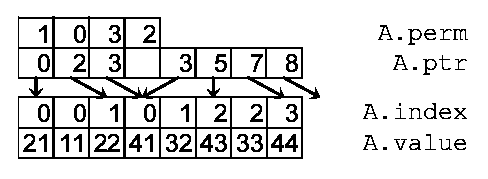
\includegraphics{storage06_omp.eps} 
\caption{JDS$B7A<0$N%G!<%?9=B$(B (OpenMP$BHG(B)}\label{fig:storage06_omp}}
\end{figure}
\begin{itembox}[l]{OpenMP$BHG(B}
\small
\begin{verbatim}
 1: int           n,nnz,maxmaxnzr,nprocs;
 2: int           *perm,*ptr,*index;
 3: LIS_SCALAR    *value;
 4: LIS_MATRIX    A;
 5: n = 4; nnz = 8; maxmaxnzr = 3; nprocs = 2;
 6: perm  = (int *)malloc( n*sizeof(int) );
 7: ptr   = (int *)malloc( nprocs*(maxmaxnzr+1)*sizeof(int) );
 8: index = (int *)malloc( nnz*sizeof(int) );
 9: value = (LIS_SCALAR *)malloc( nnz*sizeof(LIS_SCALAR) );
10: lis_matrix_create(0,&A);
11: lis_matrix_set_size(A,0,n);
12:
13: perm[0] = 1; perm[1] = 0; perm[2] = 3; perm[3] = 2;
14: ptr[0]  = 0; ptr[1]  = 2; ptr[2]  = 3; ptr[3]  = 0;
15: ptr[4]  = 3; ptr[5]  = 5; ptr[6]  = 7; ptr[7]  = 8;
16: index[0] =  0; index[1] =  0; index[2] =  1; index[3] =  0;
17: index[4] =  1; index[5] =  2; index[6] =  2; index[7] =  3;
18: value[0] = 21; value[1] = 11; value[2] = 22; value[3] = 41;
19: value[4] = 32; value[5] = 43; value[6] = 33; value[7] = 44;
20:
21:  lis_matrix_set_jds(nnz,maxmaxnzr,perm,ptr,index,value,A);
22:  lis_matrix_assemble(A);
\end{verbatim}
\end{itembox}
\newpage
\subsubsection{$B9TNs$N:n$jJ}(B (MPI$BHG(B)}
2$B%W%m%;%9>e$X$N9TNs(B$A$$B$N(BJDS$B7A<0$G$N3JG<J}K!$r?^(B\ref{fig:storage06_mpi}$B$K(B
$B<($9(B. 
2$B%W%m%;%9>e$K$3$N9TNs$r(BJDS$B7A<0$G:n@.$9$k>l9g(B, $B%W%m%0%i%`$O0J2<$N$h$&$K5-=R$9$k(B. 
\begin{figure}[h]
{\centering 
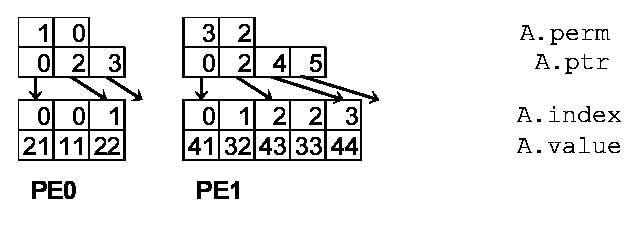
\includegraphics{storage06_mpi.eps} 
\caption{JDS$B7A<0$N%G!<%?9=B$(B (MPI$BHG(B)}\label{fig:storage06_mpi}}
\end{figure}
\begin{itembox}[l]{MPI$BHG(B}
\small
\begin{verbatim}
 1: int           i,n,nnz,maxnzr,my_rank;
 2: int           *perm,*ptr,*index;
 3: LIS_SCALAR    *value;
 4: LIS_MATRIX    A;
 5: MPI_Comm_rank(MPI_COMM_WORLD,&my_rank);
 6: if( my_rank==0 ) {n = 2; nnz = 3; maxnzr = 2;}
 7: else             {n = 2; nnz = 5; maxnzr = 3;}
 8: perm  = (int *)malloc( n*sizeof(int) );
 9: ptr   = (int *)malloc( (maxnzr+1)*sizeof(int) );
10: index = (int *)malloc( nnz*sizeof(int) );
11: value = (LIS_SCALAR *)malloc( nnz*sizeof(LIS_SCALAR) );
12: lis_matrix_create(MPI_COMM_WORLD,&A);
13: lis_matrix_set_size(A,n,0);
14: if( my_rank==0 ) {
15:     perm[0] = 1; perm[1] = 0;
16:     ptr[0]  = 0; ptr[1]  = 2; ptr[2]  = 3;
17:     index[0] =  0; index[1] =  0; index[2] =  1;
18:     value[0] = 21; value[1] = 11; value[2] = 22;}
19: else {
20:     perm[0] = 3; perm[1] = 2;
21:     ptr[0]  = 0; ptr[1]  = 2; ptr[2]  = 4; ptr[3]  = 5;
22:     index[0] =  0; index[1] =  1; index[2] =  2; index[3] =  2; index[4] =  3;
23:     value[0] = 41; value[1] = 32; value[2] = 43; value[3] = 33; value[4] = 44;}
24:  lis_matrix_set_jds(nnz,maxnzr,perm,ptr,index,value,A);
25:  lis_matrix_assemble(A);
\end{verbatim}
\end{itembox}
\subsubsection{$B4XO"$9$k4X?t(B}
\noindent
{\bf $BG[Ns$N4XO"IU$1(B}

JDS$B7A<0$KI,MW$JG[Ns$r9TNs(B$A$$B$K4XO"IU$1$k$K$O4X?t(B
\begin{itemize}
\item \verb|C       int lis_matrix_set_jds(int nnz, int maxnzr, int perm[], int ptr[],|\\
      \verb| int index[], LIS_SCALAR value[], LIS_MATRIX A)|
\item \verb|Fortran subroutine lis_matrix_set_jds(integer nnz, integer maxnzr, integer ptr(),|\\
      \verb| integer index(), LIS_SCALAR value(), LIS_MATRIX A, integer ierr)|
\end{itemize}
$B$rMQ$$$k(B. 

%%%%%%%%%%%%%%%%%%%%%%%%%%%%%%%%%%%%%%%%%%%%%%%%%%%%%%%%%%%%%%%%%%
% Block Sparse Row (BSR)
%%%%%%%%%%%%%%%%%%%%%%%%%%%%%%%%%%%%%%%%%%%%%%%%%%%%%%%%%%%%%%%%%%
\subsection{Block Sparse Row (BSR)}
BSR$B$G$O9TNs$r(B$r \times c$$B$NBg$-$5$NItJ,9TNs(B ($B%V%m%C%/$H8F$V(B) $B$KJ,2r$9$k(B. 
BSR$B$O(BCRS$B$HF1MM$N<j=g$GHsNm%V%m%C%/(B ($B>/$J$/$H$b(B1$B$D$N(B
$BHsNmMWAG$,B8:_$9$k(B) $B$r3JG<$9$k(B. 
$nr=n/r$, $nnzb$$B$r(B$A$$B$NHsNm%V%m%C%/?t$H$9$k(B. 
BSR$B$O(B3$B$D$NG[Ns(B({\ttfamily bptr, bindex, value})$B$K3JG<$9$k(B. 
\begin{itemize}
\item $BD9$5(B$nnzb \times r \times c$$B$NG\@:EYG[Ns(B{\ttfamily value}$B$OHsNm%V%m%C%/$NA4MWAG$r3JG<$9$k(B. 
\item $BD9$5(B$nnzb$$B$N@0?tG[Ns(B{\ttfamily bindex}$B$OHsNm%V%m%C%/$N%V%m%C%/NsHV9f$r3JG<$9$k(B. 
\item $BD9$5(B$nr+1$$B$N@0?tG[Ns(B{\ttfamily bptr}$B$OG[Ns(B{\ttfamily bindex}$B$N%V%m%C%/9T$N3+;O0LCV$r3JG<$9$k(B. 
\end{itemize}
\subsubsection{$B9TNs$N:n$jJ}(B ($BC`<!(B, OpenMP$BHG(B)}
$B9TNs(B$A$$B$N(BBSR$B7A<0$G$N3JG<J}K!$r?^(B\ref{fig:storage07}$B$K<($9(B. 
$B$3$N9TNs$r(BBSR$B7A<0$G:n@.$9$k>l9g(B, $B%W%m%0%i%`$O0J2<$N$h$&$K5-=R$9$k(B. 
\begin{figure}[h]
{\centering 
\begin{minipage}{0.3\textwidth}
\begin{flushright}
$ 
A = \left(
\begin{array}{cc|cc}
11 &    &    &    \\
21 & 22 &    &    \\ \hline
   & 32 & 33 &    \\
41 &    & 43 & 44 \\
\end{array}\right)
$
\end{flushright}
\end{minipage}
\begin{minipage}{0.6\textwidth}
\begin{flushleft}
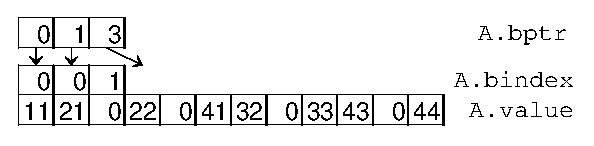
\includegraphics{storage07.eps} 
\end{flushleft}
\end{minipage}
\caption{BSR$B7A<0$N%G!<%?9=B$(B ($BC`<!(B, OpenMP$BHG(B)}\label{fig:storage07}}
\end{figure}
\begin{itembox}[l]{$BC`<!(B, OpenMP$BHG(B}
\small
\begin{verbatim}
 1: int           n,bnr,bnc,nr,nc,bnnz;
 2: int           *bptr,*bindex;
 3: LIS_SCALAR    *value;
 4: LIS_MATRIX    A;
 5: n = 4; bnr = 2; bnc = 2; bnnz = 3; nr = (n-1)/bnr+1; nc = (n-1)/bnc+1;
 6: bptr   = (int *)malloc( (nr+1)*sizeof(int) );
 7: bindex = (int *)malloc( bnnz*sizeof(int) );
 8: value  = (LIS_SCALAR *)malloc( bnr*bnc*bnnz*sizeof(LIS_SCALAR) );
 9: lis_matrix_create(0,&A);
10: lis_matrix_set_size(A,0,n);
11:
12: bptr[0] = 0; bptr[1] = 1; bptr[2] = 3;
13: bindex[0] =  0; bindex[1] =  0; bindex[2] =  1;
14: value[0]  = 11; value[1] = 21; value[2] =  0; value[3] = 22;
15: value[4]  =  0; value[5] = 41; value[6] = 32; value[7] =  0;
16: value[8]  = 33; value[9] = 43; value[10]=  0; value[11]= 44;
17:
18:  lis_matrix_set_bsr(bnr,bnc,bnnz,bptr,bindex,value,A);
19:  lis_matrix_assemble(A);
\end{verbatim}
\end{itembox}
\newpage
\subsubsection{$B9TNs$N:n$jJ}(B (MPI$BHG(B)}
2$B%W%m%;%9>e$X$N9TNs(B$A$$B$N(BBSR$B7A<0$G$N3JG<J}K!$r?^(B\ref{fig:storage07_mpi}$B$K(B
$B<($9(B. 
2$B%W%m%;%9>e$K$3$N9TNs$r(BBSR$B7A<0$G:n@.$9$k>l9g(B, $B%W%m%0%i%`$O0J2<$N$h$&$K5-=R$9$k(B. 
\begin{figure}[h]
{\centering 
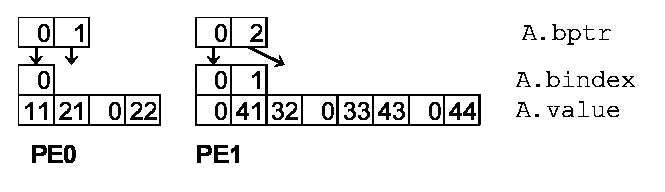
\includegraphics{storage07_mpi.eps} 
\caption{BSR$B7A<0$N%G!<%?9=B$(B (MPI$BHG(B)}\label{fig:storage07_mpi}}
\end{figure}
\begin{itembox}[l]{MPI$BHG(B}
\small
\begin{verbatim}
 1: int           n,bnr,bnc,nr,nc,bnnz,my_rank;
 2: int           *bptr,*bindex;
 3: LIS_SCALAR    *value;
 4: LIS_MATRIX    A;
 5: MPI_Comm_rank(MPI_COMM_WORLD,&my_rank);
 6: if( my_rank==0 ) {n = 2; bnr = 2; bnc = 2; bnnz = 1; nr = (n-1)/bnr+1; nc = (n-1)/bnc+1;}
 7: else             {n = 2; bnr = 2; bnc = 2; bnnz = 2; nr = (n-1)/bnr+1; nc = (n-1)/bnc+1;}
 8: bptr   = (int *)malloc( (nr+1)*sizeof(int) );
 9: bindex = (int *)malloc( bnnz*sizeof(int) );
10: value  = (LIS_SCALAR *)malloc( bnr*bnc*bnnz*sizeof(LIS_SCALAR) );
11: lis_matrix_create(MPI_COMM_WORLD,&A);
12: lis_matrix_set_size(A,n,0);
13: if( my_rank==0 ) {
14:     bptr[0] = 0; bptr[1] = 1;
15:     bindex[0] =  0;
16:     value[0]  = 11; value[1] = 21; value[2] =  0; value[3] = 22;}
17: else {
18:     bptr[0] = 0; bptr[1] = 2;
19:     bindex[0] =  0; bindex[1] =  1;
20:     value[0]  =  0; value[1]  = 41; value[2] = 32; value[3] =  0;
21:     value[4]  = 33; value[5]  = 43; value[6] =  0; value[7] = 44;}
22:  lis_matrix_set_bsr(bnr,bnc,bnnz,bptr,bindex,value,A);
23:  lis_matrix_assemble(A);
\end{verbatim}
\end{itembox}
\subsubsection{$B4XO"$9$k4X?t(B}
\noindent
{\bf $BG[Ns$N4XO"IU$1(B}

BSR$B7A<0$KI,MW$JG[Ns$r9TNs(B$A$$B$K4XO"IU$1$k$K$O4X?t(B
\begin{itemize}
\item \verb|C       int lis_matrix_set_bsr(int bnr, int bnc, int bnnz, int bptr[],|\\
      \verb| int bindex[], LIS_SCALAR value[], LIS_MATRIX A)|
\item \verb|Fortran subroutine lis_matrix_set_bsr(integer bnr, integer bnc, integer bnnz,|\\
      \verb| integer bptr(), integer bindex(), LIS_SCALAR value(), LIS_MATRIX A, integer ierr)|
\end{itemize}
$B$rMQ$$$k(B. 

%%%%%%%%%%%%%%%%%%%%%%%%%%%%%%%%%%%%%%%%%%%%%%%%%%%%%%%%%%%%%%%%%%
% Block Sparse Column (BSC)
%%%%%%%%%%%%%%%%%%%%%%%%%%%%%%%%%%%%%%%%%%%%%%%%%%%%%%%%%%%%%%%%%%
\subsection{Block Sparse Column (BSC)}
BSC$B$G$O9TNs$r(B$r \times c$$B$NBg$-$5$NItJ,9TNs(B ($B%V%m%C%/$H8F$V(B) $B$KJ,2r$9$k(B. 
BSC$B$O(BCCS$B$HF1MM$N<j=g$GHsNm%V%m%C%/(B ($B>/$J$/$H$b(B1$B$D$N(B
$BHsNmMWAG$,B8:_$9$k(B) $B$r3JG<$9$k(B. 
$nc=n/c$, $nnzb$$B$r(B$A$$B$NHsNm%V%m%C%/?t$H$9$k(B. 
BSC$B$O(B3$B$D$NG[Ns(B({\ttfamily bptr, bindex, value})$B$K3JG<$9$k(B. 
\begin{itemize}
\item $BD9$5(B$nnzb \times r \times c$$B$NG\@:EYG[Ns(B{\ttfamily value}$B$OHsNm%V%m%C%/$NA4MWAG$r3JG<$9$k(B. 
\item $BD9$5(B$nnzb$$B$N@0?tG[Ns(B{\ttfamily bindex}$B$OHsNm%V%m%C%/$N%V%m%C%/9THV9f$r3JG<$9$k(B. 
\item $BD9$5(B$nc+1$$B$N@0?tG[Ns(B{\ttfamily bptr}$B$OG[Ns(B{\ttfamily bindex}$B$N%V%m%C%/Ns$N3+;O0LCV$r3JG<$9$k(B. 
\end{itemize}
\subsubsection{$B9TNs$N:n$jJ}(B ($BC`<!(B, OpenMP$BHG(B)}
$B9TNs(B$A$$B$N(BBSC$B7A<0$G$N3JG<J}K!$r?^(B\ref{fig:storage08}$B$K<($9(B. 
$B$3$N9TNs$r(BBSC$B7A<0$G:n@.$9$k>l9g(B, $B%W%m%0%i%`$O0J2<$N$h$&$K5-=R$9$k(B. 
\begin{figure}[h]
{\centering 
\begin{minipage}{0.3\textwidth}
\begin{flushright}
$ 
A = \left(
\begin{array}{cc|cc}
11 &    &    &    \\
21 & 22 &    &    \\ \hline
   & 32 & 33 &    \\
41 &    & 43 & 44 \\
\end{array}\right)
$
\end{flushright}
\end{minipage}
\begin{minipage}{0.6\textwidth}
\begin{flushleft}
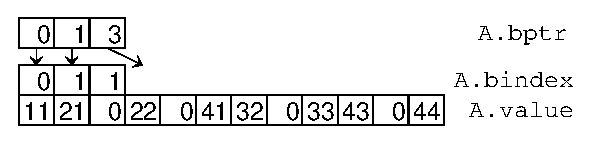
\includegraphics{storage08.eps} 
\end{flushleft}
\end{minipage}
\caption{BSC$B7A<0$N%G!<%?9=B$(B ($BC`<!(B, OpenMP$BHG(B)}\label{fig:storage08}}
\end{figure}
\begin{itembox}[l]{$BC`<!(B, OpenMP$BHG(B}
\small
\begin{verbatim}
 1: int           n,bnr,bnc,nr,nc,bnnz;
 2: int           *bptr,*bindex;
 3: LIS_SCALAR    *value;
 4: LIS_MATRIX    A;
 5: n = 4; bnr = 2; bnc = 2; bnnz = 3; nr = (n-1)/bnr+1; nc = (n-1)/bnc+1;
 6: bptr   = (int *)malloc( (nc+1)*sizeof(int) );
 7: bindex = (int *)malloc( bnnz*sizeof(int) );
 8: value  = (LIS_SCALAR *)malloc( bnr*bnc*bnnz*sizeof(LIS_SCALAR) );
 9: lis_matrix_create(0,&A);
10: lis_matrix_set_size(A,0,n);
11:
12: bptr[0] = 0; bptr[1] = 1; bptr[2] = 3;
13: bindex[0] =  0; bindex[1] =  1; bindex[2] =  1;
14: value[0]  = 11; value[1] = 21; value[2] =  0; value[3] = 22;
15: value[4]  =  0; value[5] = 41; value[6] = 32; value[7] =  0;
16: value[8]  = 33; value[9] = 43; value[10]=  0; value[11]= 44;
17:
18:  lis_matrix_set_bsc(bnr,bnc,bnnz,bptr,bindex,value,A);
19:  lis_matrix_assemble(A);
\end{verbatim}
\end{itembox}
\newpage
\subsubsection{$B9TNs$N:n$jJ}(B (MPI$BHG(B)}
2$B%W%m%;%9>e$X$N9TNs(B$A$$B$N(BBSC$B7A<0$G$N3JG<J}K!$r?^(B\ref{fig:storage08_mpi}$B$K(B
$B<($9(B. 
2$B%W%m%;%9>e$K$3$N9TNs$r(BBSC$B7A<0$G:n@.$9$k>l9g(B, $B%W%m%0%i%`$O0J2<$N$h$&$K5-=R$9$k(B. 
\begin{figure}[h]
{\centering 
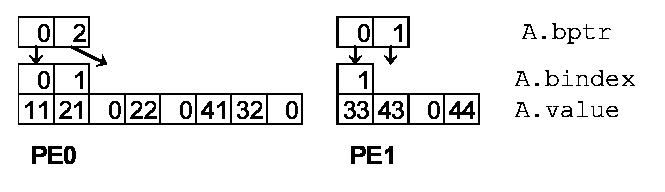
\includegraphics{storage08_mpi.eps} 
\caption{BSC$B7A<0$N%G!<%?9=B$(B (MPI$BHG(B)}\label{fig:storage08_mpi}}
\end{figure}
\begin{itembox}[l]{MPI$BHG(B}
\small
\begin{verbatim}
 1: int           n,bnr,bnc,nr,nc,bnnz,my_rank;
 2: int           *bptr,*bindex;
 3: LIS_SCALAR    *value;
 4: LIS_MATRIX    A;
 5: MPI_Comm_rank(MPI_COMM_WORLD,&my_rank);
 6: if( my_rank==0 ) {n = 2; bnr = 2; bnc = 2; bnnz = 2; nr = (n-1)/bnr+1; nc = (n-1)/bnc+1;}
 7: else             {n = 2; bnr = 2; bnc = 2; bnnz = 1; nr = (n-1)/bnr+1; nc = (n-1)/bnc+1;}
 8: bptr   = (int *)malloc( (nr+1)*sizeof(int) );
 9: bindex = (int *)malloc( bnnz*sizeof(int) );
10: value  = (LIS_SCALAR *)malloc( bnr*bnc*bnnz*sizeof(LIS_SCALAR) );
11: lis_matrix_create(MPI_COMM_WORLD,&A);
12: lis_matrix_set_size(A,n,0);
13: if( my_rank==0 ) {
14:     bptr[0] = 0; bptr[1] = 2;
15:     bindex[0] =  0; bindex[1] =  1;
16:     value[0]  = 11; value[1]  = 21; value[2] =  0; value[3] = 22;
17:     value[4]  =  0; value[5]  = 41; value[6] = 32; value[7] =  0;}
18: else {
19:     bptr[0] = 0; bptr[1] = 1;
20:     bindex[0] =  1;
21:     value[0]  = 33; value[1]  = 43; value[2] =  0; value[3] = 44;}
22:  lis_matrix_set_bsc(bnr,bnc,bnnz,bptr,bindex,value,A);
23:  lis_matrix_assemble(A);
\end{verbatim}
\end{itembox}
\subsubsection{$B4XO"$9$k4X?t(B}
\noindent
{\bf $BG[Ns$N4XO"IU$1(B}

BSC$B7A<0$KI,MW$JG[Ns$r9TNs(B$A$$B$K4XO"IU$1$k$K$O4X?t(B
\begin{itemize}
\item \verb|C       int lis_matrix_set_bsc(int bnr, int bnc, int bnnz, int bptr[],|\\
      \verb| int bindex[], LIS_SCALAR value[], LIS_MATRIX A)|
\item \verb|Fortran subroutine lis_matrix_set_bsc(integer bnr, integer bnc, integer bnnz,|\\
      \verb| integer bptr(), integer bindex(), LIS_SCALAR value(), LIS_MATRIX A, integer ierr)|
\end{itemize}
$B$rMQ$$$k(B. 

%%%%%%%%%%%%%%%%%%%%%%%%%%%%%%%%%%%%%%%%%%%%%%%%%%%%%%%%%%%%%%%%%%
% Variable Block Row (VBR)
%%%%%%%%%%%%%%%%%%%%%%%%%%%%%%%%%%%%%%%%%%%%%%%%%%%%%%%%%%%%%%%%%%
\newpage
\subsection{Variable Block Row (VBR)}
VBR$B7A<0$O(BBSR$B7A<0$r0lHL2=$7$?$b$N$G$"$k(B. 
$B9T$HNs$NJ,3d0LCV$OG[Ns(B({\ttfamily row, col})$B$GM?$($i$l$k(B. 
VBR$B$O(BCRS$B$HF1MM$N<j=g$GHsNm%V%m%C%/(B ($B>/$J$/$H$b(B1$B$D$N(B
$BHsNmMWAG$,B8:_$9$k(B) $B$r3JG<$9$k(B. 
$nr$, $nc$$B$r$=$l$>$l9TJ,3d?t(B, $BNsJ,3d?t$H$9$k(B. 
$nnzb$$B$r(B$A$$B$NHsNm%V%m%C%/?t(B, $nnz$$B$rHsNm%V%m%C%/$NA4MWAG?t$H$9$k(B. 
VBR$B$O(B6$B$D$NG[Ns(B({\ttfamily bptr, bindex, row, col, ptr, value})$B$K3JG<$9$k(B. 
\begin{itemize}
\item $BD9$5(B$nr+1$$B$N@0?tG[Ns(B{\ttfamily row}$B$O%V%m%C%/9T$N3+;O9THV9f$r3JG<$9$k(B. 
\item $BD9$5(B$nc+1$$B$N@0?tG[Ns(B{\ttfamily col}$B$O%V%m%C%/Ns$N3+;ONsHV9f$r3JG<$9$k(B. 
\item $BD9$5(B$nnzb$$B$N@0?tG[Ns(B{\ttfamily bindex}$B$OHsNm%V%m%C%/$N%V%m%C%/NsHV9f$r3JG<$9$k(B. 
\item $BD9$5(B$nr+1$$B$N@0?tG[Ns(B{\ttfamily bptr}$B$OG[Ns(B{\ttfamily bindex}$B$N%V%m%C%/9T$N3+;O0LCV$r3JG<$9$k(B. 
\item $BD9$5(B$nnz$$B$NG\@:EYG[Ns(B{\ttfamily value}$B$OHsNm%V%m%C%/$NA4MWAG$r3JG<$9$k(B. 
\item $BD9$5(B$nnzb+1$$B$N@0?tG[Ns(B{\ttfamily ptr}$B$OG[Ns(B{\ttfamily value}$B$NHsNm%V%m%C%/$N3+;O0LCV$r3JG<$9$k(B. 
\subsubsection{$B9TNs$N:n$jJ}(B ($BC`<!(B, OpenMP$BHG(B)}
$B9TNs(B$A$$B$N(BVBR$B7A<0$G$N3JG<J}K!$r?^(B\ref{fig:storage09}$B$K<($9(B. 
$B$3$N9TNs$r(BVBR$B7A<0$G:n@.$9$k>l9g(B, $B%W%m%0%i%`$O0J2<$N$h$&$K5-=R$9$k(B. 
\end{itemize}
\begin{figure}[h]
{\centering 
\begin{minipage}{0.3\textwidth}
\begin{flushright}
$ 
A = \left(
\begin{array}{c|cc|c}
11 &    &    &    \\ \hline
21 & 22 &    &    \\
   & 32 & 33 &    \\ \hline
41 &    & 43 & 44 \\
\end{array}\right)
$
\end{flushright}
\end{minipage}
\begin{minipage}{0.6\textwidth}
\begin{flushleft}
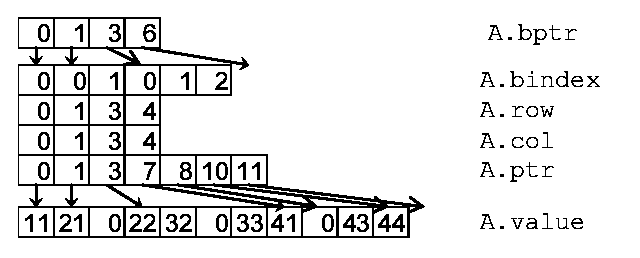
\includegraphics{storage09.eps} 
\end{flushleft}
\end{minipage}
\caption{VBR$B7A<0$N%G!<%?9=B$(B ($BC`<!(B, OpenMP$BHG(B)}\label{fig:storage09}}
\end{figure}
\begin{itembox}[l]{$BC`<!(B, OpenMP$BHG(B}
\small
\begin{verbatim}
 1: int           n,nnz,nr,nc,bnnz;
 2: int           *row,*col,*ptr,*bptr,*bindex;
 3: LIS_SCALAR    *value;
 4: LIS_MATRIX    A;
 5: n = 4; nnz = 11; bnnz = 6; nr = 3; nc = 3;
 6: bptr   = (int *)malloc( (nr+1)*sizeof(int) );
 7: row    = (int *)malloc( (nr+1)*sizeof(int) );
 8: col    = (int *)malloc( (nc+1)*sizeof(int) );
 9: ptr    = (int *)malloc( (bnnz+1)*sizeof(int) );
10: bindex = (int *)malloc( bnnz*sizeof(int) );
11: value  = (LIS_SCALAR *)malloc( nnz*sizeof(LIS_SCALAR) );
12: lis_matrix_create(0,&A);
13: lis_matrix_set_size(A,0,n);
14:
15: bptr[0] = 0; bptr[1] = 1; bptr[2] = 3; bptr[3] = 6;
16: row[0]  = 0; row[1]  = 1; row[2]  = 3; row[3] = 4;
17: col[0]  = 0; col[1]  = 1; col[2]  = 3; col[3] = 4;
18: bindex[0] =  0; bindex[1] =  0; bindex[2] =  1; bindex[3] =  0;
19: bindex[4] =  1; bindex[5] =  2;
20: ptr[0]    =  0; ptr[1]    =  1; ptr[2]    =  3; ptr[3]    =  7;
21: ptr[4]    =  8; ptr[5]    = 10; ptr[6]    = 11;
22: value[0]  = 11; value[1]  = 21; value[2]  =  0; value[3]  = 22;
23: value[4]  = 32; value[5]  =  0; value[6]  = 33; value[7]  = 41;
24: value[8]  =  0; value[9]  = 43; value[10] = 44;
25:
26:  lis_matrix_set_vbr(nnz,nr,nc,bnnz,row,col,ptr,bptr,bindex,value,A);
27:  lis_matrix_assemble(A);
\end{verbatim}
\end{itembox}
\subsubsection{$B9TNs$N:n$jJ}(B (MPI$BHG(B)}
2$B%W%m%;%9>e$X$N9TNs(B$A$$B$N(BVBR$B7A<0$G$N3JG<J}K!$r?^(B\ref{fig:storage09_mpi}$B$K(B
$B<($9(B. 
2$B%W%m%;%9>e$K$3$N9TNs$r(BVBR$B7A<0$G:n@.$9$k>l9g(B, $B%W%m%0%i%`$O0J2<$N$h$&$K5-=R$9$k(B. 
\begin{figure}[h]
{\centering 
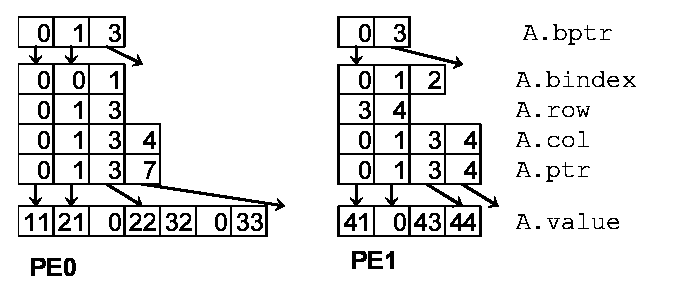
\includegraphics{storage09_mpi.eps} 
\caption{VBR$B7A<0$N%G!<%?9=B$(B ($BC`<!(B, OpenMP$BHG(B)}\label{fig:storage09_mpi}}
\end{figure}
\begin{itembox}[l]{MPI$BHG(B}
\small
\begin{verbatim}
 1: int           n,nnz,nr,nc,bnnz,my_rank;
 2: int           *row,*col,*ptr,*bptr,*bindex;
 3: LIS_SCALAR    *value;
 4: LIS_MATRIX    A;
 5: MPI_Comm_rank(MPI_COMM_WORLD,&my_rank);
 6: if( my_rank==0 ) {n = 2; nnz = 7; bnnz = 3; nr = 2; nc = 3;}
 7: else             {n = 2; nnz = 4; bnnz = 3; nr = 1; nc = 3;}
 8: bptr   = (int *)malloc( (nr+1)*sizeof(int) );
 9: row    = (int *)malloc( (nr+1)*sizeof(int) );
10: col    = (int *)malloc( (nc+1)*sizeof(int) );
11: ptr    = (int *)malloc( (bnnz+1)*sizeof(int) );
12: bindex = (int *)malloc( bnnz*sizeof(int) );
13: value  = (LIS_SCALAR *)malloc( nnz*sizeof(LIS_SCALAR) );
14: lis_matrix_create(MPI_COMM_WORLD,&A);
15: lis_matrix_set_size(A,n,0);
16: if( my_rank==0 ) {
17:     bptr[0] = 0; bptr[1] = 1; bptr[2] = 3;
18:     row[0]  = 0; row[1]  = 1; row[2]  = 3;
19:     col[0]  = 0; col[1]  = 1; col[2]  = 3; col[3] = 4;
20:     bindex[0] =  0; bindex[1] =  0; bindex[2] =  1;
21:     ptr[0]    =  0; ptr[1]    =  1; ptr[2]    =  3; ptr[3]    =  7;
22:     value[0]  = 11; value[1] = 21; value[2] =  0; value[3] = 22;
23:     value[4]  = 32; value[5] =  0; value[6] = 33;}
24: else {
25:     bptr[0] = 0; bptr[1] = 3;
26:     row[0]  = 3; row[1]  = 4;
27:     col[0]  = 0; col[1]  = 1; col[2]  = 3; col[3] = 4;
28:     bindex[0] =  0; bindex[1] =  1; bindex[2] =  2;
29:     ptr[0]    =  0; ptr[1]    =  1; ptr[2]    =  3; ptr[3]    =  4;
30:     value[0]  = 41; value[1]  =  0; value[2]  = 43; value[3]  = 44;}
31:  lis_matrix_set_vbr(nnz,nr,nc,bnnz,row,col,ptr,bptr,bindex,value,A);
32:  lis_matrix_assemble(A);
\end{verbatim}
\end{itembox}
\subsubsection{$B4XO"$9$k4X?t(B}
\noindent
{\bf $BG[Ns$N4XO"IU$1(B}

VBR$B7A<0$KI,MW$JG[Ns$r9TNs(B$A$$B$K4XO"IU$1$k$K$O4X?t(B
\begin{itemize}
\item \verb|C       int lis_matrix_set_vbr(int nnz, int nr, int nc, int bnnz, int row[],|\\
      \verb| int col[], int ptr[], int bptr[], int bindex[], LIS_SCALAR value[], LIS_MATRIX A)|
\item \verb|Fortran subroutine lis_matrix_set_vbr(integer nnz, integer nr, integer nc,|\\
      \verb| integer bnnz, integer row(), integer col(), integer ptr(), integer bptr(),|\\ 
      \verb| integer bindex(), LIS_SCALAR value(), LIS_MATRIX A, integer ierr) |
\end{itemize}
$B$rMQ$$$k(B. 

%%%%%%%%%%%%%%%%%%%%%%%%%%%%%%%%%%%%%%%%%%%%%%%%%%%%%%%%%%%%%%%%%%
% Coordinate (COO)
%%%%%%%%%%%%%%%%%%%%%%%%%%%%%%%%%%%%%%%%%%%%%%%%%%%%%%%%%%%%%%%%%%
\newpage
\subsection{Coordinate (COO)}
COO$B$O(B3$B$D$NG[Ns(B({\ttfamily row, col, value})$B$K3JG<$9$k(B. 
\begin{itemize}
\item $BD9$5(B$nnz$$B$NG\@:EYG[Ns(B{\ttfamily value}$B$OHsNmMWAG$r3JG<$9$k(B. 
\item $BD9$5(B$nnz$$B$N@0?tG[Ns(B{\ttfamily row}$B$OHsNmMWAG$N9THV9f$r3JG<$9$k(B. 
\item $BD9$5(B$nnz$$B$N@0?tG[Ns(B{\ttfamily col}$B$OHsNmMWAG$NNsHV9f$r3JG<$9$k(B. 
\end{itemize}
\subsubsection{$B9TNs$N:n$jJ}(B ($BC`<!(B, OpenMP$BHG(B)}
$B9TNs(B$A$$B$N(BCOO$B7A<0$G$N3JG<J}K!$r?^(B\ref{fig:storage10}$B$K<($9(B. 
$B$3$N9TNs$r(BCOO$B7A<0$G:n@.$9$k>l9g(B, $B%W%m%0%i%`$O0J2<$N$h$&$K5-=R$9$k(B. 
\begin{figure}[h]
{\centering 
\begin{minipage}{0.3\textwidth}
\begin{flushright}
$ 
A = \left(
\begin{array}{cccc}
11 &    &    &    \\
21 & 22 &    &    \\
   & 32 & 33 &    \\
41 &    & 43 & 44 \\
\end{array}\right)
$
\end{flushright}
\end{minipage}
\begin{minipage}{0.6\textwidth}
\begin{flushleft}
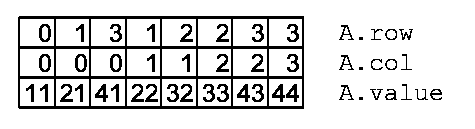
\includegraphics{storage10.eps} 
\end{flushleft}
\end{minipage}
\caption{COO$B7A<0$N%G!<%?9=B$(B ($BC`<!(B, OpenMP$BHG(B)}\label{fig:storage10}}
\end{figure}
\begin{itembox}[l]{$BC`<!(B, OpenMP$BHG(B}
\small
\begin{verbatim}
 1: int           n,nnz;
 2: int           *row,*col;
 3: LIS_SCALAR    *value;
 4: LIS_MATRIX    A;
 5: n = 4; nnz = 8;
 6: row   = (int *)malloc( nnz*sizeof(int) );
 7: col   = (int *)malloc( nnz*sizeof(int) );
 8: value = (LIS_SCALAR *)malloc( nnz*sizeof(LIS_SCALAR) );
 9: lis_matrix_create(0,&A);
10: lis_matrix_set_size(A,0,n);
11:
12: row[0] = 0; row[1] = 1; row[2] = 3; row[3] = 1;
13: row[4] = 2; row[5] = 2; row[6] = 3; row[7] = 3;
14: col[0] = 0; col[1] = 0; col[2] = 0; col[3] = 1;
15: col[4] = 1; col[5] = 2; col[6] = 2; col[7] = 3;
16: value[0] = 11; value[1] = 21; value[2] = 41; value[3] = 22;
17: value[4] = 32; value[5] = 33; value[6] = 43; value[7] = 44;
18:
19:  lis_matrix_set_coo(nnz,row,col,value,A);
20:  lis_matrix_assemble(A);
\end{verbatim}
\end{itembox}
\newpage
\subsubsection{$B9TNs$N:n$jJ}(B (MPI$BHG(B)}
2$B%W%m%;%9>e$X$N9TNs(B$A$$B$N(BCOO$B7A<0$G$N3JG<J}K!$r?^(B\ref{fig:storage10_mpi}$B$K(B
$B<($9(B. 
2$B%W%m%;%9>e$K$3$N9TNs$r(BCOO$B7A<0$G:n@.$9$k>l9g(B, $B%W%m%0%i%`$O0J2<$N$h$&$K5-=R$9$k(B. 
\begin{figure}[h]
{\centering 
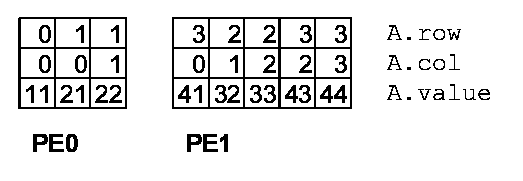
\includegraphics{storage10_mpi.eps} 
\caption{COO$B7A<0$N%G!<%?9=B$(B (MPI$BHG(B)}\label{fig:storage10_mpi}}
\end{figure}
\begin{itembox}[l]{MPI$BHG(B}
\small
\begin{verbatim}
 1: int           n,nnz,my_rank;
 2: int           *row,*col;
 3: LIS_SCALAR    *value;
 4: LIS_MATRIX    A;
 5: MPI_Comm_rank(MPI_COMM_WORLD,&my_rank);
 6: if( my_rank==0 ) {n = 2; nnz = 3;}
 7: else             {n = 2; nnz = 5;}
 8: row   = (int *)malloc( nnz*sizeof(int) );
 9: col   = (int *)malloc( nnz*sizeof(int) );
10: value = (LIS_SCALAR *)malloc( nnz*sizeof(LIS_SCALAR) );
11: lis_matrix_create(MPI_COMM_WORLD,&A);
12: lis_matrix_set_size(A,n,0);
13: if( my_rank==0 ) {
14:     row[0] = 0; row[1] = 1; row[2] = 1;
15:     col[0] = 0; col[1] = 0; col[2] = 1;
16:     value[0] = 11; value[1] = 21; value[2] = 22;}
17: else {
18:     row[0] = 3; row[1] = 2; row[2] = 2; row[3] = 3; row[4] = 3;
19:     col[0] = 0; col[1] = 1; col[2] = 2; col[3] = 2; col[4] = 3;
20:     value[0] = 41; value[1] = 32; value[2] = 33; value[3] = 43; value[4] = 44;}
21:  lis_matrix_set_coo(nnz,row,col,value,A);
22:  lis_matrix_assemble(A);
\end{verbatim}
\end{itembox}
\subsubsection{$B4XO"$9$k4X?t(B}
\noindent
{\bf $BG[Ns$N4XO"IU$1(B}

COO$B7A<0$KI,MW$JG[Ns$r9TNs(B$A$$B$K4XO"IU$1$k$K$O4X?t(B
\begin{itemize}
\item \verb|C       int lis_matrix_set_coo(int nnz, int row[], int col[], LIS_SCALAR value[],|\\
      \verb| LIS_MATRIX A)|
\item \verb|Fortran subroutine lis_matrix_set_coo(integer nnz, integer row(), integer col(),|\\
      \verb| LIS_SCALAR value(), LIS_MATRIX A, integer ierr)|
\end{itemize}
$B$rMQ$$$k(B. 

%%%%%%%%%%%%%%%%%%%%%%%%%%%%%%%%%%%%%%%%%%%%%%%%%%%%%%%%%%%%%%%%%%
% Dense (DNS)
%%%%%%%%%%%%%%%%%%%%%%%%%%%%%%%%%%%%%%%%%%%%%%%%%%%%%%%%%%%%%%%%%%
\newpage
\subsection{Dense (DNS)}
DNS$B$O(B1$B$D$NG[Ns(B({\ttfamily value})$B$K3JG<$9$k(B. 
\begin{itemize}
\item $BD9$5(B$n \times n$$B$NG\@:EYG[Ns(B{\ttfamily value}$B$ONsM%@h$GMWAG$r3JG<$9$k(B. 
\end{itemize}
\subsubsection{$B9TNs$N:n$jJ}(B ($BC`<!(B, OpenMP$BHG(B)}
$B9TNs(B$A$$B$N(BDNS$B7A<0$G$N3JG<J}K!$r?^(B\ref{fig:storage11}$B$K<($9(B. 
$B$3$N9TNs$r(BDNS$B7A<0$G:n@.$9$k>l9g(B, $B%W%m%0%i%`$O0J2<$N$h$&$K5-=R$9$k(B. 
\begin{figure}[h]
{\centering 
\begin{minipage}{0.3\textwidth}
\begin{flushright}
$ 
A = \left(
\begin{array}{cccc}
11 &    &    &    \\
21 & 22 &    &    \\
   & 32 & 33 &    \\
41 &    & 43 & 44 \\
\end{array}\right)
$
\end{flushright}
\end{minipage}
\begin{minipage}{0.6\textwidth}
\begin{flushleft}
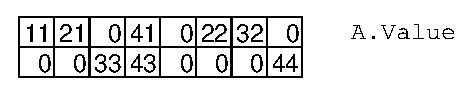
\includegraphics{storage11.eps} 
\end{flushleft}
\end{minipage}
\caption{DNS$B7A<0$N%G!<%?9=B$(B ($BC`<!(B, OpenMP$BHG(B)}\label{fig:storage11}}
\end{figure}
\begin{itembox}[l]{$BC`<!(B, OpenMP$BHG(B}
\small
\begin{verbatim}
 1: int           n;
 2: LIS_SCALAR    *value;
 3: LIS_MATRIX    A;
 4: n = 4;
 5: value = (LIS_SCALAR *)malloc( n*n*sizeof(LIS_SCALAR) );
 6: lis_matrix_create(0,&A);
 7: lis_matrix_set_size(A,0,n);
 8:
 9: value[0] = 11; value[1] = 21; value[2] =  0; value[3] = 41;
10: value[4] =  0; value[5] = 22; value[6] = 32; value[7] =  0;
11: value[8] =  0; value[9] =  0; value[10]= 33; value[11]= 43;
12: value[12]=  0; value[13]=  0; value[14]=  0; value[15]= 44;
13:
14:  lis_matrix_set_dns(value,A);
15:  lis_matrix_assemble(A);
\end{verbatim}
\end{itembox}
\newpage
\subsubsection{$B9TNs$N:n$jJ}(B (MPI$BHG(B)}
2$B%W%m%;%9>e$X$N9TNs(B$A$$B$N(BDNS$B7A<0$G$N3JG<J}K!$r?^(B\ref{fig:storage11_mpi}$B$K(B
$B<($9(B. 
2$B%W%m%;%9>e$K$3$N9TNs$r(BDNS$B7A<0$G:n@.$9$k>l9g(B, $B%W%m%0%i%`$O0J2<$N$h$&$K5-=R$9$k(B. 
\begin{figure}[h]
{\centering 
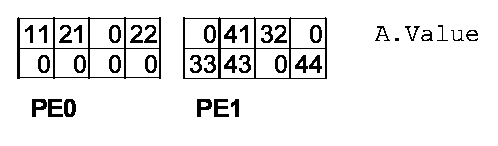
\includegraphics{storage11_mpi.eps} 
\caption{DNS$B7A<0$N%G!<%?9=B$(B (MPI$BHG(B)}\label{fig:storage11_mpi}}
\end{figure}
\begin{itembox}[l]{MPI$BHG(B}
\small
\begin{verbatim}
 1: int           n,my_rank;
 2: LIS_SCALAR    *value;
 3: LIS_MATRIX    A;
 4: MPI_Comm_rank(MPI_COMM_WORLD,&my_rank);
 5: if( my_rank==0 ) {n = 2;}
 6: else             {n = 2;}
 7: value = (LIS_SCALAR *)malloc( n*n*sizeof(LIS_SCALAR) );
 8: lis_matrix_create(MPI_COMM_WORLD,&A);
 9: lis_matrix_set_size(A,n,0);
10: if( my_rank==0 ) {
11:     value[0] = 11; value[1] = 21; value[2] =  0; value[3] = 22;
12:     value[4] =  0; value[5] =  0; value[6] =  0; value[7] =  0;}
13: else {
14:     value[0] =  0; value[1] = 41; value[2] = 32; value[3] =  0;
15:     value[4] = 33; value[5] = 43; value[6] =  0; value[7] = 44;}
16:  lis_matrix_set_dns(value,A);
17:  lis_matrix_assemble(A);
\end{verbatim}
\end{itembox}
\subsubsection{$B4XO"$9$k4X?t(B}
\noindent
{\bf $BG[Ns$N4XO"IU$1(B}

DNS$B7A<0$KI,MW$JG[Ns$r9TNs(B$A$$B$K4XO"IU$1$k$K$O4X?t(B
\begin{itemize}
\item \verb|C       int lis_matrix_set_dns(LIS_SCALAR value[], LIS_MATRIX A)|
\item \verb|Fortran subroutine lis_matrix_set_dns(LIS_SCALAR value(), LIS_MATRIX A, integer ierr)|
\end{itemize}
$B$rMQ$$$k(B. 

%%%%%%%%%%%%%%%%%%%%%%%%%%%%%%%%%%%%%%%%%%%%%%%%%%%%%%%%%%%%%%
%%%%%%%%%%%%%%%%%%%%%%%%%%%%%%%%%%%%%%%%%%%%%%%%%%%%%%%%%%%%%%
%%%%%%%%%%%%%%%%%%%%%%%%%%%%%%%%%%%%%%%%%%%%%%%%%%%%%%%%%%%%%%
\newpage
\section{$B4X?t(B}\label{sec:func}
$BK\@a$G$O(B, $B%f!<%6$,;HMQ$G$-$k4X?t$K$D$$$F=R$Y$k(B. 
$B4X?t$N2r@b$O(BC$B$r4p=`$K5-=R$7$F$$$k(B. $BG[Ns$O(BC$B$G$O(B0$B%*%j%8%s(B, Fortran$B$G$O(B1$B%*%j%8%s$G$"$k(B. 
$B$J$*(B, C$B$G$N3F4X?t$NLa$jCM(B, Fortran$B$G$N(B{\tt ierr}$B$NCM$O0J2<$N$h$&$K$J$C$F$$$k(B. 
\\ \\ \\
{\bf $BLa$jCM(B}
\begin{namelist}{XXXXXXXXXXXXXXXXXXXX}
\item[\tt LIS\_SUCCESS(0)] ~~~~~$B@5>o=*N;(B
\item[\tt LIS\_ILL\_OPTION(1)] ~~~~~$B%*%W%7%g%s$,IT@5(B
\item[\tt LIS\_BREAKDOWN(2)] ~~~~~$B%V%l%$%/%@%&%s(B
\item[\tt LIS\_OUT\_OF\_MEMORY(3)] ~~~~~$B%a%b%jITB-(B
\item[\tt LIS\_MAXITER(4)] ~~~~~$B:GBgH?I|2s?t$^$G$K<}B+$7$J$+$C$?(B
\item[\tt LIS\_NOT\_IMPLEMENTED(5)] ~~~~~$B$^$@<BAu$5$l$F$$$J$$(B
\item[\tt LIS\_ERR\_FILE\_IO(6)] ~~~~~$B%U%!%$%k(BI/O$B%(%i!<(B
\end{namelist}

%%%%%%%%%%%%%%%%%%%%%%%%%%%%%%%%%%%%%%%%%%%%%%%%%%%%%%%%%%%%%%
\subsection{$B%Y%/%H%kA`:n(B}
$B%Y%/%H%k(B$v$$B$N<!?t$r(B$global\_n$$B$H$9$k(B. 
$B%Y%/%H%k(B$v$$B$r(B$nprocs$$B8D$N%W%m%;%9$G9T%V%m%C%/J,3d$7$?$H$-$N(B
$B3F%V%m%C%/$N9T?t$r(B$local\_n$$B$H$9$k(B. 
$global\_n$$B$r%0%m!<%P%k$J<!?t(B, $local\_n$$B$r%m!<%+%k$J<!?t$H8F$V(B. 
%%%%%%%%%%%%%%%%%%%%%%%%%%%%%%%%%%%%%%%%%%%%%%%%%%%%%%%%%%%%%%
\subsubsection{lis\_vector\_create}
\begin{screen}
\verb|C       int lis_vector_create(LIS_Comm comm, LIS_VECTOR *vec)|\\
\verb|Fortran subroutine lis_vector_create(LIS_Comm comm, LIS_VECTOR vec, integer ierr)| 
\end{screen}
{\bf $B5!G=(B}\\
\indent
$B%Y%/%H%k$r:n@.$9$k(B. 
\\ \\
\noindent
{\bf $BF~NO(B}
\begin{namelist}{XXXXXXXXXXXXXXXXXXXX}
\item[\tt LIS\_Comm] MPI$B%3%_%e%K%1!<%?(B
\end{namelist}
{\bf $B=PNO(B}
\begin{namelist}{XXXXXXXXXXXXXXXXXXXX}
\item[\tt vec] $B%Y%/%H%k(B
\item[\tt ierr] $B%j%?!<%s%3!<%I(B
\end{namelist}
{\bf $BCm<a(B}\\
\indent
$BC`<!(B, OpenMP$BHG$G$O(B, {\tt comm}$B$NCM$OL5;k$5$l$k(B. 

%%%%%%%%%%%%%%%%%%%%%%%%%%%%%%%%%%%%%%%%%%%%%%%%%%%%%%%%%%%%%%
  \subsubsection{lis\_vector\_destroy}
\begin{screen}
\verb|C       int lis_vector_destroy(LIS_VECTOR vec)|\\
\verb|Fortran subroutine lis_vector_destroy(LIS_VECTOR vec, integer ierr)|
\end{screen}
{\bf $B5!G=(B}\\
\indent
$BITMW$K$J$C$?%Y%/%H%k$r%a%b%j$+$iGK4~$9$k(B. 
\\ \\
\noindent
{\bf $BF~NO(B}
\begin{namelist}{XXXXXXXXXXXXXXXXXXXX}
\item[\tt vec] $B%a%b%j$+$iGK4~$9$k%Y%/%H%k(B
\end{namelist}
{\bf $B=PNO(B}
\begin{namelist}{XXXXXXXXXXXXXXXXXXXX}
\item[\tt ierr] $B%j%?!<%s%3!<%I(B
\end{namelist}
%%%%%%%%%%%%%%%%%%%%%%%%%%%%%%%%%%%%%%%%%%%%%%%%%%%%%%%%%%%%%%
  \subsubsection{lis\_vector\_duplicate}
\begin{screen}
\verb|C       int lis_vector_duplicate(void *vin, LIS_VECTOR *vout)|
\verb|Fortran subroutine lis_vector_duplicate(LIS_VECTOR vin, LIS_VECTOR vout,|\\
\verb|         integer ierr)|
\end{screen}
{\bf $B5!G=(B}\\
\indent
$B4{B8$N%Y%/%H%k$^$?$O9TNs$HF1$8>pJs$r;}$D%Y%/%H%k$r:n@.$9$k(B. 
\\ \\
\noindent
{\bf $BF~NO(B}
\begin{namelist}{XXXXXXXXXXXXXXXXXXXX}
\item[\tt vin] $BJ#@=85$N%Y%/%H%k$^$?$O9TNs(B
\end{namelist}
{\bf $B=PNO(B}
\begin{namelist}{XXXXXXXXXXXXXXXXXXXX}
\item[\tt vout] $BJ#@=@h$N%Y%/%H%k(B
\item[\tt ierr] $B%j%?!<%s%3!<%I(B
\end{namelist}
{\bf $BCm<a(B}\\
\indent
\verb|vin|$B$K$O(B\verb|LIS_VECOTR|$B$^$?$O(B\verb|LIS_MATRIX|$B$r;XDj$9$k$3$H$,2DG=$G$"$k(B. 
\verb|lis_vector_duplicate|$B4X?t$OCM$O%3%T!<$5$l$:(B, $BNN0h$N$_3NJ]$5$l$k(B. 
$BCM$b%3%T!<$7$?$$>l9g$O$3$N4X?t$N8e$K(B
\verb|lis_vector_copy|$B4X?t$rMQ$$$k(B. 
%%%%%%%%%%%%%%%%%%%%%%%%%%%%%%%%%%%%%%%%%%%%%%%%%%%%%%%%%%%%%%
\newpage
\subsubsection{lis\_vector\_set\_size}
\begin{screen}
\verb|C       int lis_vector_set_size(LIS_VECTOR vec, int local_n, int global_n)|\\
\verb|Fortran subroutine lis_vector_set_size(LIS_VECTOR vec, integer local_n,|\\
\verb|         integer global_n, integer ierr)| 
\end{screen}
{\bf $B5!G=(B}\\
\indent
$B%Y%/%H%k$N%5%$%:$r@_Dj$9$k(B.
\\ \\
\noindent
{\bf $BF~NO(B}
\begin{namelist}{XXXXXXXXXXXXXXXXXXXX}
\item[\tt vec] $B%Y%/%H%k(B
\item[\tt local\_n] $B%Y%/%H%k$N%m!<%+%k$J<!?t(B
\item[\tt global\_n] $B%Y%/%H%k$N%0%m!<%P%k$J<!?t(B
\end{namelist}
{\bf $B=PNO(B}
\begin{namelist}{XXXXXXXXXXXXXXXXXXXX}
\item[\tt ierr] $B%j%?!<%s%3!<%I(B
\end{namelist}
{\bf $BCm<a(B}\\
\indent
$local\_n$ $B$+(B $global\_n$ $B$N$I$A$i$+0lJ}$rM?$($J$1$l$P$J$i$J$$(B. 
$BC`<!(B, OpenMP$BHG$G$O(B, $B%Y%/%H%k$N<!?t$O(B$local\_n$ $=$ $global\_n$$B$H$J$k(B. 
$B$7$?$,$C$F(B, \\
\verb|lis_vector_set_size(v,n,0)|
$B$H(B\verb|lis_vector_set_size(v,0,n)|$B$O$I$A$i$b<!?t(B$n$$B$N%Y%/%H%k$r:n@.$9$k$3$H$r0UL#$9$k(B. 

MPI$BHG$G$O(B, \verb|lis_vector_set_size(v,n,0)|$B$H$9$k$H(B, 
$B3F%W%m%;%9(B$p$$B$K<!?t(B$n_p$$B$NItJ,%Y%/%H%k$r:n@.$9$k(B. 
$B0lJ}(B, \verb|lis_vector_set_size(v,0,n)|$B$H$9$k$H(B
$B3F%W%m%;%9(B$p$$B$K<!?t(B$m_p$$B$NItJ,%Y%/%H%k$r:n@.$9$k(B. $B$?$@$7(B, $m_p$$B$NCM$O%i%$%V%i%jB&$G7hDj$5$l$k(B. 
%%%%%%%%%%%%%%%%%%%%%%%%%%%%%%%%%%%%%%%%%%%%%%%%%%%%%%%%%%%%%%
\newpage
  \subsubsection{lis\_vector\_get\_size}
\begin{screen}
\verb|C       int lis_vector_get_size(LIS_VECTOR v, int *local_n, int *global_n)|
\verb|Fortran subroutine lis_vector_get_size(LIS_VECTOR v, integer local_n,|\\
\verb|         integer global_n, integer ierr)|
\end{screen}
{\bf $B5!G=(B}\\
\indent
$B%Y%/%H%k(B$v$$B$N%5%$%:$rF@$k(B. 
\\ \\
\noindent
{\bf $BF~NO(B}
\begin{namelist}{XXXXXXXXXXXXXXXXXXXX}
\item[\tt v] $B%Y%/%H%k(B
\end{namelist}
{\bf $B=PNO(B}
\begin{namelist}{XXXXXXXXXXXXXXXXXXXX}
\item[\tt local\_n] $B%Y%/%H%k$N%m!<%+%k$J<!?t(B
\item[\tt global\_n] $B%Y%/%H%k$N%0%m!<%P%k$J<!?t(B
\item[\tt ierr] $B%j%?!<%s%3!<%I(B
\end{namelist}
{\bf $BCm<a(B}\\
\indent
$BC`<!(B, OpenMP$BHG$G$O(B, $local\_n$ $=$ $global\_n$ $B$H$J$k(B. 
%%%%%%%%%%%%%%%%%%%%%%%%%%%%%%%%%%%%%%%%%%%%%%%%%%%%%%%%%%%%%%
  \subsubsection{lis\_vector\_get\_range}
\begin{screen}
\verb|C       int lis_vector_get_range(LIS_VECTOR v, int *is, int *ie)|
\verb|Fortran subroutine lis_vector_get_range(LIS_VECTOR v, integer is, integer ie,|\\
\verb|         integer ierr) |
\end{screen}
{\bf $B5!G=(B}\\
\indent
$BItJ,%Y%/%H%k(B$v$$B$,A4BN%Y%/%H%k$N$I$3$K0LCV$7$F$$$k$N$+$rD4$Y$k(B. 
\\ \\
\noindent
{\bf $BF~NO(B}
\begin{namelist}{XXXXXXXXXXXXXXXXXXXX}
\item[\tt v] $BItJ,%Y%/%H%k(B
\end{namelist}
{\bf $B=PNO(B}
\begin{namelist}{XXXXXXXXXXXXXXXXXXXX}
\item[\tt is] $BItJ,%Y%/%H%k(B$v$$B$NA4BN%Y%/%H%kCf$G$N3+;O0LCV(B
\item[\tt ie] $BItJ,%Y%/%H%k(B$v$$B$NA4BN%Y%/%H%kCf$G$N=*N;0LCV(B+1
\item[\tt ierr] $B%j%?!<%s%3!<%I(B
\end{namelist}
{\bf $BCm<a(B}\\
\indent
$BC`<!(B, OpenMP$BHG$G$O(B, $n$$B<!%Y%/%H%k$G$O(B$is=0$, $ie=n$ $B$H$J$k(B. 
%%%%%%%%%%%%%%%%%%%%%%%%%%%%%%%%%%%%%%%%%%%%%%%%%%%%%%%%%%%%%%
  \subsubsection{lis\_vector\_set\_value}
\begin{screen}
\verb|C       int lis_vector_set_value(int flag, int i, LIS_SCALAR value, LIS_VECTOR v)|
\verb|Fortran subroutine lis_vector_set_value(integer flag, integer i, LIS_SCALAR value,|\\
\verb|         LIS_VECTOR v, integer ierr)|
\end{screen}
{\bf $B5!G=(B}\\
\indent
$B%Y%/%H%k(B$v$$B$N(B$i$$B9TL\$K%9%+%iCM(B$value$$B$rBeF~$9$k(B. 
\\ \\
\noindent
{\bf $BF~NO(B}
\begin{namelist}{XXXXXXXXXXXXXXXXXXXX}
\item[\tt flag] \begin{description}
\item[\tt LIS\_INS\_VALUE] $BA^F~(B    : {\tt v[$i$] = $value$}
\item[\tt LIS\_ADD\_VALUE] $B2C;;BeF~(B: {\tt v[$i$] = v[$i$] + $value$}
\end{description}
\item[\tt i] $BBeF~$9$k>l=j(B
\item[\tt value] $BBeF~$9$k%9%+%iCM(B
\item[\tt v] $BBeF~$5$l$k%Y%/%H%k(B
\end{namelist}
{\bf $B=PNO(B}
\begin{namelist}{XXXXXXXXXXXXXXXXXXXX}
\item[\tt v] $i$$B9TL\$K%9%+%iCM(B$value$$B$,BeF~$5$l$?%Y%/%H%k(B
\item[\tt ierr] $B%j%?!<%s%3!<%I(B
\end{namelist}
{\bf $BCm<a(B}\\
\indent
MPI$BHG$G$O(B, $BItJ,%Y%/%H%k$N(B$i$$B9TL\$G$O$J$/A4BN%Y%/%H%k$N(B$i$$B9TL\$r;XDj$9$k(B. 
%%%%%%%%%%%%%%%%%%%%%%%%%%%%%%%%%%%%%%%%%%%%%%%%%%%%%%%%%%%%%%
  \subsubsection{lis\_vector\_get\_value}
\begin{screen}
\verb|C       int lis_vector_get_value(LIS_VECTOR v, int i, LIS_SCALAR *value)|
\verb|Fortran subroutine lis_vector_get_value(LIS_VECTOR v, integer i, LIS_SCALAR value,|\\
\verb|         integer ierr)|
\end{screen}
{\bf $B5!G=(B}\\
\indent
$B%Y%/%H%k(B$v$$B$N(B$i$$B9TL\$NCM$r(B$value$$B$K<hF@$9$k(B. 
\\ \\
\noindent
{\bf $BF~NO(B}
\begin{namelist}{XXXXXXXXXXXXXXXXXXXX}
\item[\tt i] $B<hF@$9$k>l=j(B
\item[\tt v] $BCM$r<hF@$9$k%Y%/%H%k(B
\end{namelist}
{\bf $B=PNO(B}
\begin{namelist}{XXXXXXXXXXXXXXXXXXXX}
\item[\tt value] $B%9%+%iCM(B
\item[\tt ierr] $B%j%?!<%s%3!<%I(B
\end{namelist}
{\bf $BCm<a(B}\\
\indent
MPI$BHG$G$O(B, $BItJ,%Y%/%H%k$N(B$i$$B9TL\$G$O$J$/A4BN%Y%/%H%k$N(B$i$$B9TL\$r;XDj$9$k(B. 
%%%%%%%%%%%%%%%%%%%%%%%%%%%%%%%%%%%%%%%%%%%%%%%%%%%%%%%%%%%%%%
  \subsubsection{lis\_vector\_set\_values}
\begin{screen}
\verb|C       int lis_vector_set_values(int flag, int count, int index[],|\\
\verb|         LIS_SCALAR value[], LIS_VECTOR v)|\\
\verb|Fortran subroutine lis_vector_set_values(integer flag, integer count,|\\
\verb|         integer index(), LIS_SCALAR value(), LIS_VECTOR v, integer ierr)|
\end{screen}
{\bf $B5!G=(B}\\
\indent
$B%Y%/%H%k(B$v$$B$N(B{\tt index[$i$]}$B9TL\$K%9%+%iCM(B{\tt value[$i$]}$B$rBeF~$9$k(B. 
\\ \\
\noindent
{\bf $BF~NO(B}
\begin{namelist}{XXXXXXXXXXXXXXXXXXXX}
\item[\tt flag] \begin{description}
\item[\tt LIS\_INS\_VALUE] $BA^F~(B    : {\tt v[index[$i$]] = value[$i$]}
\item[\tt LIS\_ADD\_VALUE] $B2C;;BeF~(B: {\tt v[index[$i$]] = v[index[$i$]] + value[$i$]}
\end{description}
\item[\tt count] $BBeF~$9$k%9%+%iCM$r3JG<$9$kG[Ns$NMWAG?t(B
\item[\tt index] $BBeF~$9$k>l=j$r3JG<$9$kG[Ns(B
\item[\tt value] $BBeF~$9$k%9%+%iCM$r3JG<$9$kG[Ns(B
\item[\tt v] $BBeF~$5$l$k%Y%/%H%k(B
\end{namelist}
{\bf $B=PNO(B}
\begin{namelist}{XXXXXXXXXXXXXXXXXXXX}
\item[\tt v] {\tt index[$i$]}$B9TL\$K%9%+%iCM(B{\tt value[$i$]}$B$,BeF~$5$l$?%Y%/%H%k(B
\item[\tt ierr] $B%j%?!<%s%3!<%I(B
\end{namelist}
{\bf $BCm<a(B}\\
\indent
MPI$BHG$G$O(B, $BItJ,%Y%/%H%k$N(B{\tt index[$i$]}$B9TL\$G$O$J$/A4BN%Y%/%H%k$N(B{\tt index[$i$]}$B9TL\$r;XDj$9$k(B. 
%%%%%%%%%%%%%%%%%%%%%%%%%%%%%%%%%%%%%%%%%%%%%%%%%%%%%%%%%%%%%%
\newpage
  \subsubsection{lis\_vector\_get\_values}
\begin{screen}
\verb|C       int lis_vector_get_values(LIS_VECTOR v, int start, int count,|\\
\verb|         LIS_SCALAR value[])|\\
\verb|Fortran subroutine lis_vector_get_values(LIS_VECTOR v, integer start,|\\
\verb|         integer count, LIS_SCALAR value(), integer ierr)|
\end{screen}
{\bf $B5!G=(B}\\
\indent
$B%Y%/%H%k(B$v$$B$N(B$start+i$$B9TL\$NCM(B ($i=0,1,..., count-1$)$B$r(B{\tt
value[$i$]}$B$K3JG<$9$k(B. 
\\ \\
\noindent
{\bf $BF~NO(B}
\begin{namelist}{XXXXXXXXXXXXXXXXXXXX}
\item[\tt start] $B<hF@$9$k>l=j$N;OE@(B
\item[\tt count] $B<hF@$9$k%9%+%iCM$N8D?t(B
\item[\tt v] $BCM$r<hF@$9$k%Y%/%H%k(B
\end{namelist}
{\bf $B=PNO(B}
\begin{namelist}{XXXXXXXXXXXXXXXXXXXX}
\item[\tt value] $B<hF@$7$?%9%+%iCM$r3JG<$9$k%Y%/%H%k(B
\item[\tt ierr] $B%j%?!<%s%3!<%I(B
\end{namelist}
{\bf $BCm<a(B}\\
\indent
MPI$BHG$G$O(B, $BItJ,%Y%/%H%k$N(B$start+i$$B9TL\$G$O$J$/A4BN%Y%/%H%k$N(B$start+i$$B9TL\$r;XDj$9$k(B. 
%%%%%%%%%%%%%%%%%%%%%%%%%%%%%%%%%%%%%%%%%%%%%%%%%%%%%%%%%%%%%%
\newpage
  \subsubsection{lis\_vector\_scatter}
\begin{screen}
\verb|C       int lis_vector_scatter(LIS_SCALAR value[], LIS_VECTOR v)|\\
\verb|Fortran subroutine lis_vector_scatter(LIS_SCALAR value(), LIS_VECTOR v, integer ierr)|
\end{screen}
{\bf $B5!G=(B}\\
\indent
$B%Y%/%H%k(B$v$$B$N(B$i$$B9TL\$NCM(B ($i=0,1,...,global\_n-1$)$B$r(B{\tt value[$i$]}$B$+$i<hF@$9$k(B. 
\\ \\
\noindent
{\bf $BF~NO(B}
\begin{namelist}{XXXXXXXXXXXXXXXXXXXX}
\item[\tt value] $B<hF@$9$k%9%+%iCM$r3JG<$9$k%Y%/%H%k(B
\end{namelist}
{\bf $B=PNO(B}
\begin{namelist}{XXXXXXXXXXXXXXXXXXXX}
\item[\tt v] $BCM$r<hF@$7$?%Y%/%H%k(B
\item[\tt ierr] $B%j%?!<%s%3!<%I(B
\end{namelist}
\indent
%%%%%%%%%%%%%%%%%%%%%%%%%%%%%%%%%%%%%%%%%%%%%%%%%%%%%%%%%%%%%%
  \subsubsection{lis\_vector\_gather}
\begin{screen}
\verb|C       int lis_vector_gather(LIS_VECTOR v, LIS_SCALAR value[])|\\
\verb|Fortran subroutine lis_vector_gather(LIS_VECTOR v, LIS_SCALAR value(), integer ierr)|
\end{screen}
{\bf $B5!G=(B}\\
\indent
$B%Y%/%H%k(B{\tt v}$B$N(B$i$$B9TL\$NCM(B ($i=0,1,..., global\_n-1$)$B$r(B{\tt
value[$i$]}$B$K3JG<$9$k(B. 
\\ \\
\noindent
{\bf $BF~NO(B}
\begin{namelist}{XXXXXXXXXXXXXXXXXXXX}
\item[\tt v] $BCM$r<hF@$9$k%Y%/%H%k(B
\end{namelist}
{\bf $B=PNO(B}
\begin{namelist}{XXXXXXXXXXXXXXXXXXXX}
\item[\tt value] $B<hF@$7$?%9%+%iCM$r3JG<$9$k%Y%/%H%k(B
\item[\tt ierr] $B%j%?!<%s%3!<%I(B
\end{namelist}
\indent
%%%%%%%%%%%%%%%%%%%%%%%%%%%%%%%%%%%%%%%%%%%%%%%%%%%%%%%%%%%%%%
\newpage
  \subsubsection{lis\_vector\_copy}
\begin{screen}
\verb|C       int lis_vector_copy(LIS_VECTOR x, LIS_VECTOR y)|\\
\verb|Fortran subroutine lis_vector_copy(LIS_VECTOR x, LIS_VECTOR y, integer ierr)|
\end{screen}
{\bf $B5!G=(B}\\
\indent
$B%Y%/%H%k$NMWAG$r%3%T!<$9$k(B. 
\\ \\
\noindent
{\bf $BF~NO(B}
\begin{namelist}{XXXXXXXXXXXXXXXXXXXX}
\item[\tt x] $B%3%T!<85%Y%/%H%k(B
\end{namelist}
{\bf $B=PNO(B}
\begin{namelist}{XXXXXXXXXXXXXXXXXXXX}
\item[\tt y] $B%3%T!<@h%Y%/%H%k(B
\item[\tt ierr] $B%j%?!<%s%3!<%I(B
\end{namelist}
%%%%%%%%%%%%%%%%%%%%%%%%%%%%%%%%%%%%%%%%%%%%%%%%%%%%%%%%%%%%%%
  \subsubsection{lis\_vector\_set\_all}
\begin{screen}
\verb|C       int lis_vector_set_all(LIS_SCALAR value, LIS_VECTOR x)|
\verb|Fortran subroutine lis_vector_set_all(LIS_SCALAR value, LIS_VECTOR x, integer ierr)|
\end{screen}
{\bf $B5!G=(B}\\
\indent
$B%Y%/%H%k$N$9$Y$F$NMWAG$K%9%+%iCM(B$value$$B$rBeF~$9$k(B. 
\\ \\
\noindent
{\bf $BF~NO(B}
\begin{namelist}{XXXXXXXXXXXXXXXXXXXX}
\item[\tt value] $BBeF~$9$k%9%+%iCM(B
\item[\tt v] $BBeF~$5$l$k%Y%/%H%k(B
\end{namelist}
{\bf $B=PNO(B}
\begin{namelist}{XXXXXXXXXXXXXXXXXXXX}
\item[\tt v] $B$9$Y$F$NMWAG$K(B$value$$B$,BeF~$5$l$?%Y%/%H%k(B
\item[\tt ierr] $B%j%?!<%s%3!<%I(B
\end{namelist}
%%%%%%%%%%%%%%%%%%%%%%%%%%%%%%%%%%%%%%%%%%%%%%%%%%%%%%%%%%%%%%
%%%%%%%%%%%%%%%%%%%%%%%%%%%%%%%%%%%%%%%%%%%%%%%%%%%%%%%%%%%%%%
\newpage
  \subsubsection{lis\_vector\_is\_null}
\begin{screen}
\verb|C       int lis_vector_is_null(LIS_VECTOR v)|\\
\verb|Fortran subroutine lis_vector_is_null(LIS_VECTOR v,integer ierr)|
\end{screen}
{\bf $B5!G=(B}\\
\indent
$B%Y%/%H%k(B$v$$B$,MxMQ2DG=$+$I$&$+$rD4$Y$k(B. 
\\ \\
\noindent
{\bf $BF~NO(B}
\begin{namelist}{XXXXXXXXXXXXXXXXXXXX}
\item[\tt v] $B%Y%/%H%k(B
\end{namelist}
{\bf $B=PNO(B}
\begin{namelist}{XXXXXXXXXXXXXXXXXXXX}
\item[\tt ierr] \begin{description}
\item[\tt LIS\_TRUE] $BMxMQ2DG=(B
\item[\tt LIS\_FALSE] $BMxMQIT2D(B
\end{description}
\end{namelist}
%%%%%%%%%%%%%%%%%%%%%%%%%%%%%%%%%%%%%%%%%%%%%%%%%%%%%%%%%%%%%%
\newpage
\subsection{$B9TNsA`:n(B}
$B9TNs(B$A$$B$N<!?t$r(B$global\_n$ $\times$ $global\_n$$B$H$9$k(B. 
$B9TNs(B$A$$B$r(B$nprocs$$B8D$N%W%m%;%9$G9T%V%m%C%/J,3d$7$?$H$-$N(B
$B3FItJ,9TNs$N9T?t$r(B$local\_n$$B$H$9$k(B. 
$global\_n$$B$r%0%m!<%P%k$J9T?t(B, $local\_n$$B$r%m!<%+%k$J9T?t$H8F$V(B. 
  \subsubsection{lis\_matrix\_create}
\begin{screen}
\verb|C       int lis_matrix_create(LIS_Comm comm, LIS_MATRIX *A)|
\verb|Fortran subroutine lis_matrix_create(LIS_Comm comm, LIS_MATRIX A, integer ierr)|
\end{screen}
{\bf $B5!G=(B}\\
\indent
$B9TNs$r:n@.$9$k(B. 
\\ \\
\noindent
{\bf $BF~NO(B}
\begin{namelist}{XXXXXXXXXXXXXXXXXXXX}
\item[\tt LIS\_Comm] MPI$B%3%_%e%K%1!<%?(B
\end{namelist}
{\bf $B=PNO(B}
\begin{namelist}{XXXXXXXXXXXXXXXXXXXX}
\item[\tt A] $B9TNs(B
\item[\tt ierr] $B%j%?!<%s%3!<%I(B
\end{namelist}
{\bf $BCm<a(B}\\
\indent
$BC`<!(B, OpenMP$BHG$G$O(B, {\tt comm}$B$NCM$OL5;k$5$l$k(B. 
%%%%%%%%%%%%%%%%%%%%%%%%%%%%%%%%%%%%%%%%%%%%%%%%%%%%%%%%%%%%%%
  \subsubsection{lis\_matrix\_destroy}
\begin{screen}
\verb|C       int lis_matrix_destroy(LIS_MATRIX A)|\\
\verb|Fortran subroutine lis_matrix_destroy(LIS_MATRIX A, integer ierr)|
\end{screen}
{\bf $B5!G=(B}\\
\indent
$BITMW$K$J$C$?9TNs$r%a%b%j$+$iGK4~$9$k(B. 
\\ \\
\noindent
{\bf $BF~NO(B}
\begin{namelist}{XXXXXXXXXXXXXXXXXXXX}
\item[\tt A] $B%a%b%j$+$iGK4~$9$k9TNs(B
\end{namelist}
{\bf $B=PNO(B}
\begin{namelist}{XXXXXXXXXXXXXXXXXXXX}
\item[\tt ierr] $B%j%?!<%s%3!<%I(B
\end{namelist}
%%%%%%%%%%%%%%%%%%%%%%%%%%%%%%%%%%%%%%%%%%%%%%%%%%%%%%%%%%%%%%
  \subsubsection{lis\_matrix\_duplicate}
\begin{screen}
\verb|C       int lis_matrix_duplicate(LIS_MATRIX Ain, LIS_MATRIX *Aout)|
\verb|Fortran subroutine lis_matrix_duplicate(LIS_MATRIX Ain, LIS_MATRIX Aout,|\\
\verb|         integer ierr)|
\end{screen}
{\bf $B5!G=(B}\\
\indent
$B4{B8$N9TNs$HF1$8>pJs$r;}$D9TNs$r:n@.$9$k(B. 
\\ \\
\noindent
{\bf $BF~NO(B}
\begin{namelist}{XXXXXXXXXXXXXXXXXXXX}
\item[\tt Ain] $BJ#@=85$N9TNs(B
\end{namelist}
{\bf $B=PNO(B}
\begin{namelist}{XXXXXXXXXXXXXXXXXXXX}
\item[\tt Aout] $BJ#@=@h$N9TNs(B
\item[\tt ierr] $B%j%?!<%s%3!<%I(B
\end{namelist}
{\bf $BCm<a(B}\\
\indent
\verb|lis_matrix_duplicate|$B4X?t$O9TNs$NMWAG$NCM$O%3%T!<$5$l$:(B, $BNN0h$N$_3NJ]$5$l$k(B. 
$BMWAG$NCM$b%3%T!<$7$?$$>l9g$O(B\verb|lis_matrix_copy|$B4X?t$rMQ$$$k(B. 
%%%%%%%%%%%%%%%%%%%%%%%%%%%%%%%%%%%%%%%%%%%%%%%%%%%%%%%%%%%%%%
  \subsubsection{lis\_matrix\_malloc}
\begin{screen}
\verb|C       int lis_matrix_malloc(LIS_MATRIX A, int nnz_row, int nnz[])|
\verb|Fortran subroutine lis_matrix_malloc(LIS_MATRIX A, integer nnz_row, integer nnz[],|\\
\verb|         integer ierr)|
\end{screen}
{\bf $B5!G=(B}\\
\indent
$B9TNs$NNN0h$r3NJ]$9$k(B. 
\\ \\
\noindent
{\bf $BF~NO(B}
\begin{namelist}{XXXXXXXXXXXXXXXXXXXX}
\item[\tt A] $B9TNs(B
\item[\tt nnz\_row] $BJ?6QHsNmMWAG?t(B
\item[\tt nnz] $B3F9T$NHsNmMWAG?t$NG[Ns(B
\end{namelist}
{\bf $B=PNO(B}
\begin{namelist}{XXXXXXXXXXXXXXXXXXXX}
\item[\tt ierr] $B%j%?!<%s%3!<%I(B
\end{namelist}
{\bf $BCm<a(B}\\
\indent
$nnz\_row$ $B$^$?$O(B $nnz$ $B$N$I$A$i$+0lJ}$r;XDj$9$k(B. 
$B$3$N4X?t$O(B, \verb|lis_matrix_set_value| $B$G8zN($h$/MWAG$rBeF~$G$-$k$h$&$K(B, $B$"$i$+$8$a(B
$BNN0h$r3NJ]$9$k(B. 
%%%%%%%%%%%%%%%%%%%%%%%%%%%%%%%%%%%%%%%%%%%%%%%%%%%%%%%%%%%%%%
  \subsubsection{lis\_matrix\_set\_value}
\begin{screen}
\verb|C       int lis_matrix_set_value(int flag, int i, int j, LIS_SCALAR value,|\\
\verb|         LIS_MATRIX A)|\\
\verb|Fortran subroutine lis_matrix_set_value(integer flag, integer i, integer j,|\\
\verb|         LIS_SCALAR value, LIS_MATRIX A, integer ierr)|
\end{screen}
{\bf $B5!G=(B}\\
\indent
$B9TNs(B$A$$B$N(B$i$$B9T(B$j$$BNsL\$KMWAG$rBeF~$9$k(B. 
\\ \\
\noindent
{\bf $BF~NO(B}
\begin{namelist}{XXXXXXXXXXXXXXXXXXXX}
\item[\tt flag] \begin{description}
\item[\tt LIS\_INS\_VALUE] $BA^F~(B    : {$A(i,j) = value$}
\item[\tt LIS\_ADD\_VALUE] $B2C;;BeF~(B: {$A(i,j) = A(i,j) + value$}
\end{description}
\item[\tt i] $B9TNs$N9THV9f(B
\item[\tt j] $B9TNs$NNsHV9f(B
\item[\tt value] $BBeF~$9$k%9%+%iCM(B
\item[\tt A] $B9TNs(B
\end{namelist}
{\bf $B=PNO(B}
\begin{namelist}{XXXXXXXXXXXXXXXXXXXX}
\item[\tt A] $i$$B9T(B$j$$BNsL\$KMWAG$,BeF~$5$l$?9TNs(B
\item[\tt ierr] $B%j%?!<%s%3!<%I(B
\end{namelist}
\noindent
{\bf $BCm<a(B}\\
\indent
MPI$BHG$G$O(B, $BItJ,9TNs$N(B$i$$B9T(B$j$$BNsL\$G$O$J$/A4BN9TNs$N(B$i$$B9T(B$j$$BNsL\$r;XDj$9$k(B. 

\verb|lis_matrix_set_value|$B4X?t$OBeF~$5$l$?CM$r0l;~E*$JFbIt7A<0$G(B
$B3JG<$9$k$?$a(B, \verb|lis_matrix_set_value|$B$rMQ$$$?8e$K$OI,$:(B
\verb|lis_matrix_assemble|$B4X?t$r8F$S=P$5$J$1$l$P$J$i$J$$(B. 
%%%%%%%%%%%%%%%%%%%%%%%%%%%%%%%%%%%%%%%%%%%%%%%%%%%%%%%%%%%%%%
  \subsubsection{lis\_matrix\_assemble}
\begin{screen}
\verb|C       int lis_matrix_assemble(LIS_MATRIX A)|\\
\verb|Fortran subroutine lis_matrix_assemble(LIS_MATRIX A, integer ierr)|
\end{screen}
{\bf $B5!G=(B}\\
\indent
$B9TNs$r%i%$%V%i%j$GMxMQ2DG=$K$9$k(B. 
\\ \\
\noindent
{\bf $BF~NO(B}
\begin{namelist}{XXXXXXXXXXXXXXXXXXXX}
\item[\tt A] $B9TNs(B
\end{namelist}
{\bf $B=PNO(B}
\begin{namelist}{XXXXXXXXXXXXXXXXXXXX}
\item[\tt A] $BMxMQ2DG=$K$J$C$?9TNs(B
\item[\tt ierr] $B%j%?!<%s%3!<%I(B
\end{namelist}
%%%%%%%%%%%%%%%%%%%%%%%%%%%%%%%%%%%%%%%%%%%%%%%%%%%%%%%%%%%%%%
  \subsubsection{lis\_matrix\_set\_size}
\begin{screen}
\verb|int lis_matrix_set_size(LIS_MATRIX A, int local_n, int global_n)|
\verb|Fortran subroutine lis_matrix_set_size(LIS_MATRIX A, integer local_n,|\\
\verb|         integer global_n, integer ierr)|
\end{screen}
{\bf $B5!G=(B}\\
\indent
$B9TNs$N%5%$%:$r@_Dj$9$k(B. 
\\ \\
\noindent
{\bf $BF~NO(B}
\begin{namelist}{XXXXXXXXXXXXXXXXXXXX}
\item[\tt A] $B9TNs(B
\item[\tt local\_n] $B9TNs(B$A$$B$N%m!<%+%k$J9T?t(B
\item[\tt global\_n] $B9TNs(B$A$$B$N%0%m!<%P%k$J9T?t(B
\end{namelist}
{\bf $B=PNO(B}
\begin{namelist}{XXXXXXXXXXXXXXXXXXXX}
\item[\tt ierr] $B%j%?!<%s%3!<%I(B
\end{namelist}
{\bf $BCm<a(B}\\
\indent
$local\_n$ $B$+(B $global\_n$ $B$N$I$A$i$+0lJ}$rM?$($J$1$l$P$J$i$J$$(B. 

$BC`<!(B, OpenMP$BHG$G$O(B, $B9TNs$N%5%$%:$O(B$local\_n$ $=$ $global\_n$$B$H$J$k(B. 
$B$7$?$,$C$F(B, \\
\verb|lis_matrix_set_size(A,n,0)|
$B$H(B\verb|lis_matrix_set_size(A,0,n)|$B$O$H$b$K(B$n \times n$$B$N%5%$%:$r@_Dj$9$k$3$H$r0UL#$9$k(B. 

MPI$BHG$G$O(B, \verb|lis_matrix_set_size(A,n,0)|$B$H$9$k$H(B, 
$B3F%W%m%;%9(B$p$$B$G9TNs%5%$%:$,(B$n_p \times N$$B$H$J$k$h$&$K@_Dj$9$k(B. $B$3$3$G(B,
$N$$B$O3F%W%m%;%9$N(B$n_p$$B$NAmOB$G$"$k(B. \\
$B0lJ}(B, \verb|lis_matrix_set_size(A,0,n)|$B$H$9$k$H(B
$B3F%W%m%;%9(B$p$$B$G9TNs%5%$%:$,(B$m_p \times n$$B$H$J$k$h$&$K@_Dj$9$k(B. $B$3$3$G(B, $m_p$$B$OItJ,9TNs$N9T?t$G(B
$B$3$NCM$O%i%$%V%i%jB&$G7hDj$5$l$k(B. 
%%%%%%%%%%%%%%%%%%%%%%%%%%%%%%%%%%%%%%%%%%%%%%%%%%%%%%%%%%%%%%
\newpage
  \subsubsection{lis\_matrix\_get\_size}
\begin{screen}
\verb|C       int lis_matrix_get_size(LIS_MATRIX A, int *local_n, int *global_n)|
\verb|Fortran subroutine lis_matrix_get_size(LIS_MATRIX A, integer local_n,|\\
\verb|         integer global_n, integer ierr)|
\end{screen}
{\bf $B5!G=(B}\\
\indent
$B9TNs$N%5%$%:$r<hF@$9$k(B. 
\\ \\
\noindent
{\bf $BF~NO(B}
\begin{namelist}{XXXXXXXXXXXXXXXXXXXX}
\item[\tt A] $B9TNs(B
\end{namelist}
{\bf $B=PNO(B}
\begin{namelist}{XXXXXXXXXXXXXXXXXXXX}
\item[\tt local\_n] $B9TNs(B$A$$B$N%m!<%+%k$J9T?t(B
\item[\tt global\_n] $B9TNs(B$A$$B$N%0%m!<%P%k$J9T?t(B
\item[\tt ierr] $B%j%?!<%s%3!<%I(B
\end{namelist}
{\bf $BCm<a(B}\\
\indent
$BC`<!(B, OpenMP$BHG$G$O(B, $local\_n$ $=$ $global\_n$ $B$H$J$k(B. 
%%%%%%%%%%%%%%%%%%%%%%%%%%%%%%%%%%%%%%%%%%%%%%%%%%%%%%%%%%%%%%
  \subsubsection{lis\_matrix\_get\_range}
\begin{screen}
\verb|C       int lis_matrix_get_range(LIS_MATRIX A, int *is, int *ie)|
\verb|Fortran subroutine lis_matrix_get_range(LIS_MATRIX A, integer is, integer ie,|\\
\verb|         integer ierr)|
\end{screen}
{\bf $B5!G=(B}\\
\indent
$BItJ,9TNs(B$A$$B$,A4BN9TNs$N$I$3$K0LCV$7$F$$$k$N$+$rD4$Y$k(B. 
\\ \\
\noindent
{\bf $BF~NO(B}
\begin{namelist}{XXXXXXXXXXXXXXXXXXXX}
\item[\tt A] $BItJ,9TNs(B
\end{namelist}
{\bf $B=PNO(B}
\begin{namelist}{XXXXXXXXXXXXXXXXXXXX}
\item[\tt is] $BItJ,9TNs(B$A$$B$NA4BN9TNsCf$G$N3+;O0LCV(B
\item[\tt ie] $BItJ,9TNs(B$A$$B$NA4BN9TNsCf$G$N=*N;0LCV(B+1
\item[\tt ierr] $B%j%?!<%s%3!<%I(B
\end{namelist}
{\bf $BCm<a(B}\\
\indent
$BC`<!(B, OpenMP$BHG$G$O(B, $n \times n$$B9TNs$G$O(B$is=0$, $ie=n$$B$H$J$k(B. 
%%%%%%%%%%%%%%%%%%%%%%%%%%%%%%%%%%%%%%%%%%%%%%%%%%%%%%%%%%%%%%
  \subsubsection{lis\_matrix\_set\_type}
\begin{screen}
\verb|C       int lis_matrix_set_type(LIS_MATRIX A, int matrix_type)|
\verb|Fortran subroutine lis_matrix_set_type(LIS_MATRIX A, int matrix_type, integer ierr)|
\end{screen}
{\bf $B5!G=(B}\\
\indent
$B9TNs$N3JG<7A<0$r@_Dj$9$k(B. 
\\ \\
\noindent
{\bf $BF~NO(B}
\begin{namelist}{XXXXXXXXXXXXXXXXXXXX}
\item[\tt A] $B9TNs(B
\item[\tt matrix\_type] $B9TNs$N3JG<7A<0(B
\end{namelist}
{\bf $B=PNO(B}
\begin{namelist}{XXXXXXXXXXXXXXXXXXXX}
\item[\tt ierr] $B%j%?!<%s%3!<%I(B
\end{namelist}
\noindent
{\bf $BCm<a(B}\\
\indent
$B9TNs:n@.;~$K(B$A$$B$N(B \verb+matrix_type+ $B$O(B \verb+LIS_MATRIX_CRS+ $B$H$J$C$F$$$k(B. 
$B0J2<$K(B \verb+matrix_type+ $B$K;XDj2DG=$J3JG<7A<0$r<($9(B. 
\\ \\
\begin{minipage}[t]{\textwidth}
\begin{center}
\begin{tabular}{lll}\hline\hline
$B3JG<7A<0(B  & & matrix\_type \\ \hline
Compressed Row Storage & (CRS) & \verb|LIS_MATRIX_CRS| \\
Compressed Column Storage & (CCS) & \verb|LIS_MATRIX_CCS| \\
Modified Compressed Sparse Row & (MSR) & \verb|LIS_MATRIX_MSR| \\
Diagonal &(DIA) & \verb|LIS_MATRIX_DIA| \\
Ellpack-Itpack generalized diagonal &(ELL) & \verb|LIS_MATRIX_ELL| \\
Jagged Diagonal &(JDS) & \verb|LIS_MATRIX_JDS| \\
Block Sparse Row & (BSR) & \verb|LIS_MATRIX_BSR| \\
Block Sparse Column &(BSC) & \verb|LIS_MATRIX_BSC| \\
Variable Block Row &(VBR) & \verb|LIS_MATRIX_VBR| \\
Dense &	(DNS) & \verb|LIS_MATRIX_DNS| \\
Coordinate & (COO) & \verb|LIS_MATRIX_COO| \\
\hline         
\end{tabular}
\end{center}
\end{minipage}
%%%%%%%%%%%%%%%%%%%%%%%%%%%%%%%%%%%%%%%%%%%%%%%%%%%%%%%%%%%%%%
\newpage
  \subsubsection{lis\_matrix\_get\_type}
\begin{screen}
\verb|C       int lis_matrix_get_type(LIS_MATRIX A, int *matrix_type)|
\verb|Fortran subroutine lis_matrix_get_type(LIS_MATRIX A, integer matrix_type,|\\
\verb|         integer ierr)|
\end{screen}
{\bf $B5!G=(B}\\
\indent
$B9TNs$N3JG<7A<0$r<hF@$9$k(B. 
\\ \\
\noindent
{\bf $BF~NO(B}
\begin{namelist}{XXXXXXXXXXXXXXXXXXXX}
\item[\tt A] $B9TNs(B
\end{namelist}
{\bf $B=PNO(B}
\begin{namelist}{XXXXXXXXXXXXXXXXXXXX}
\item[\tt matrix\_type] $B9TNs$N3JG<7A<0(B
\item[\tt ierr] $B%j%?!<%s%3!<%I(B
\end{namelist}
%%%%%%%%%%%%%%%%%%%%%%%%%%%%%%%%%%%%%%%%%%%%%%%%%%%%%%%%%%%%%%
  \subsubsection{lis\_matrix\_set\_blocksize}
\begin{screen}
\verb|C       int lis_matrix_set_blocksize(LIS_MATRIX A, int bnr, int bnc, int row[],|\\
\verb|         int col[])|\\
\verb|Fortran subroutine lis_matrix_set_blocksize(LIS_MATRIX A, integer bnr, integer bnc,|\\
\verb|         integer row[], integer col[], integer ierr)|
\end{screen}
{\bf $B5!G=(B}\\
\indent
BSR, BSC, VBR$B$N%V%m%C%/%5%$%:(B, $BJ,3d>pJs$r@_Dj$9$k(B. 
\\ \\
\noindent
{\bf $BF~NO(B}
\begin{namelist}{XXXXXXXXXXXXXXXXXXXX}
\item[\tt A] $B9TNs(B
\item[\tt bnr] BSR(BSC)$B$N9T%V%m%C%/%5%$%:(B, $B$^$?$O(BVBR$B$N9T%V%m%C%/?t(B
\item[\tt bnc] BSR(BSC)$B$NNs%V%m%C%/%5%$%:(B, $B$^$?$O(BVBR$B$NNs%V%m%C%/?t(B
\item[\tt row] VBR$B$N9TJ,3d>pJs$NG[Ns(B
\item[\tt col] VBR$B$NNsJ,3d>pJs$NG[Ns(B
\end{namelist}
{\bf $B=PNO(B}
\begin{namelist}{XXXXXXXXXXXXXXXXXXXX}
\item[\tt ierr] $B%j%?!<%s%3!<%I(B
\end{namelist}
%%%%%%%%%%%%%%%%%%%%%%%%%%%%%%%%%%%%%%%%%%%%%%%%%%%%%%%%%%%%%%
  \subsubsection{lis\_matrix\_convert}
\begin{screen}
\verb|C       int lis_matrix_convert(LIS_MATRIX Ain, LIS_MATRIX Aout)|\\
\verb|Fortran subroutine lis_matrix_convert(LIS_MATRIX Ain, LIS_MATRIX Aout, integer ierr)|
\end{screen}
{\bf $B5!G=(B}\\
\indent
$B9TNs(B$Ain$$B$r;XDj$N3JG<7A<0$KJQ49$7$?9TNs(B$Aout$$B$r:n@.$9$k(B. 
\\ \\
\noindent
{\bf $BF~NO(B}
\begin{namelist}{XXXXXXXXXXXXXXXXXXXX}
\item[\tt Ain] $BJQ4985$N9TNs(B
\end{namelist}
{\bf $B=PNO(B}
\begin{namelist}{XXXXXXXXXXXXXXXXXXXX}
\item[\tt Aout] $B;XDj$N3JG<7A<0$KJQ49$5$l$?9TNs(B
\item[\tt ierr] $B%j%?!<%s%3!<%I(B
\end{namelist}
{\bf $BCm<a(B}\\
\indent
$BJQ49$9$k3JG<7A<0$N;XDj$O(B \verb|lis_matrix_set_type| 
$B$rMQ$$$F(B \verb|Aout| $B$K@_Dj$9$k(B. 
BSR, BSC, VBR$B$N%V%m%C%/%5%$%:Ey$N>pJs$O%f!<%6$,(B \verb|lis_matrix_set_blocksize| $B$r(B
$BMQ$$$F(B \verb|Aout| $B$K@_Dj$9$k(B. 

$B85$N9TNs$+$i;XDj$N3JG<7A<0$X$NJQ49$G0J2<$NI=$N!{$H$J$C$F$$$k7PO)$OD>@\JQ49$5$l(B, 
$B$=$l0J30$O5-:\$5$l$F$$$k7A<0$r7PM3$7$F$+$i;XDj$N3JG<7A<0$KJQ49$5$l$k(B. 
$B$^$?(B, $BI=$K5-:\$5$l$F$$$J$$7PO)$O(BCRS$B$r7PM3$7$F$+$i;XDj$N3JG<7A<0$KJQ49$5$l$k(B.  
\\ \vspace*{5mm}

\begin{tabular}{|c|c|c|c|c|c|c|c|c|c|c|c|}
\hline
$B85!@@h(B & CRS & CCS & MSR & DIA & ELL & JDS & BSR & BSC & VBR & DNS & COO \\ \hline
CRS    &     &  $B!{(B  &  $B!{(B  &  $B!{(B  &  $B!{(B  &  $B!{(B  &  $B!{(B  &  CCS  &  $B!{(B  &  $B!{(B  &  $B!{(B  \\ \hline
COO    &  $B!{(B  &  $B!{(B  &  $B!{(B  & CRS  & CRS & CRS & CRS & CCS & CRS & CRS &    \\ \hline
\end{tabular}
%%%%%%%%%%%%%%%%%%%%%%%%%%%%%%%%%%%%%%%%%%%%%%%%%%%%%%%%%%%%%%
  \subsubsection{lis\_matrix\_copy}
\begin{screen}
\verb|C       int lis_matrix_copy(LIS_MATRIX Ain, LIS_MATRIX Aout)|
\verb|Fortran subroutine lis_matrix_copy(LIS_MATRIX Ain, LIS_MATRIX Aout, integer ierr) |
\end{screen}
{\bf $B5!G=(B}\\
\indent
$B9TNs$NMWAG$r%3%T!<$9$k(B. 
\\ \\
\noindent
{\bf $BF~NO(B}
\begin{namelist}{XXXXXXXXXXXXXXXXXXXX}
\item[\tt Ain] $B%3%T!<85$N9TNs(B
\end{namelist}
{\bf $B=PNO(B}
\begin{namelist}{XXXXXXXXXXXXXXXXXXXX}
\item[\tt Aout] $B%3%T!<@h$N9TNs(B
\item[\tt ierr] $B%j%?!<%s%3!<%I(B
\end{namelist}
%%%%%%%%%%%%%%%%%%%%%%%%%%%%%%%%%%%%%%%%%%%%%%%%%%%%%%%%%%%%%%
  \subsubsection{lis\_matrix\_get\_diagonal}
\begin{screen}
\verb|C       int lis_matrix_get_diagonal(LIS_MATRIX A, LIS_VECTOR d)|\\
\verb|Fortran subroutine lis_matrix_get_diagonal(LIS_MATRIX A, LIS_VECTOR d, integer ierr) |
\end{screen}
{\bf $B5!G=(B}\\
\indent
$B9TNs(B$A$$B$NBP3QItJ,$r%Y%/%H%k(B$d$$B$K%3%T!<$9$k(B. 
\\ \\
\noindent
{\bf $BF~NO(B}
\begin{namelist}{XXXXXXXXXXXXXXXXXXXX}
\item[\tt A] $B9TNs(B
\end{namelist}
{\bf $B=PNO(B}
\begin{namelist}{XXXXXXXXXXXXXXXXXXXX}
\item[\tt d] $BBP3QMWAG$,3JG<$5$l$?%Y%/%H%k(B
\item[\tt ierr] $B%j%?!<%s%3!<%I(B
\end{namelist}
%%%%%%%%%%%%%%%%%%%%%%%%%%%%%%%%%%%%%%%%%%%%%%%%%%%%%%%%%%%%%%
\newpage
  \subsubsection{lis\_matrix\_set\_crs}
\begin{screen}
\verb|C       int lis_matrix_set_crs(int nnz, int ptr[], int index[], LIS_SCALAR value[],|\\
\verb|         LIS_MATRIX A)|\\
\verb|Fortran subroutine lis_matrix_set_crs(integer nnz, integer row(), integer index(),|\\
\verb|         LIS_SCALAR value(), LIS_MATRIX A, integer ierr)|

\end{screen}
{\bf $B5!G=(B}\\
\indent
$B%f!<%6<+?H$,:n@.$7$?(BCRS$B7A<0$KI,MW$JG[Ns$r9TNs(B$A$$B$K4XO"IU$1$k(B. 
\\ \\
\noindent
{\bf $BF~NO(B}
\begin{namelist}{XXXXXXXXXXXXXXXXXXXX}
\item[\tt nnz] $BHsNmMWAG?t(B
\item[\tt ptr, index, value] CRS$B7A<0$NG[Ns(B
\item[\tt A] $B9TNs(B
\end{namelist}
{\bf $B=PNO(B}
\begin{namelist}{XXXXXXXXXXXXXXXXXXXX}
\item[\tt A] $B4XO"IU$1$i$l$?9TNs(B
\end{namelist}
\noindent
{\bf $BCm<a(B}\\
\indent
\verb|lis_matrix_set_crs|$B$rMQ$$$?8e$K$OI,$:(B
\verb|lis_matrix_assemble|$B$r8F$S=P$5$J$1$l$P$J$i$J$$(B. 
%%%%%%%%%%%%%%%%%%%%%%%%%%%%%%%%%%%%%%%%%%%%%%%%%%%%%%%%%%%%%%
  \subsubsection{lis\_matrix\_set\_ccs}
\begin{screen}
\verb|C       int lis_matrix_set_ccs(int nnz, int ptr[], int index[], LIS_SCALAR value[],|\\
\verb|         LIS_MATRIX A)|\\
\verb|Fortran subroutine lis_matrix_set_ccs(integer nnz, integer row(), integer index(),|\\
\verb|         LIS_SCALAR value(), LIS_MATRIX A, integer ierr)|
\end{screen}
{\bf $B5!G=(B}\\
\indent
$B%f!<%6<+?H$,:n@.$7$?(BCCS$B7A<0$KI,MW$JG[Ns$r9TNs(B$A$$B$K4XO"IU$1$k(B. 
\\ \\
\noindent
{\bf $BF~NO(B}
\begin{namelist}{XXXXXXXXXXXXXXXXXXXX}
\item[\tt nnz] $BHsNmMWAG?t(B
\item[\tt ptr, index, value] CCS$B7A<0$NG[Ns(B
\item[\tt A] $B9TNs(B
\end{namelist}
{\bf $B=PNO(B}
\begin{namelist}{XXXXXXXXXXXXXXXXXXXX}
\item[\tt A] $B4XO"IU$1$i$l$?9TNs(B
\end{namelist}
\noindent
{\bf $BCm<a(B}\\
\indent
\verb|lis_matrix_set_ccs|$B$rMQ$$$?8e$K$OI,$:(B
\verb|lis_matrix_assemble|$B$r8F$S=P$5$J$1$l$P$J$i$J$$(B. 
%%%%%%%%%%%%%%%%%%%%%%%%%%%%%%%%%%%%%%%%%%%%%%%%%%%%%%%%%%%%%%
  \subsubsection{lis\_matrix\_set\_msr}
\begin{screen}
\verb|C       int lis_matrix_set_msr(int nnz, int ndz, int index[], LIS_SCALAR value[],|\\
\verb|         LIS_MATRIX A)| \\
\verb|Fortran subroutine lis_matrix_set_msr(integer nnz, integer ndz, integer index(),|\\
\verb|         LIS_SCALAR value(), LIS_MATRIX A, integer ierr)|
\end{screen}
{\bf $B5!G=(B}\\
\indent
$B%f!<%6<+?H$,:n@.$7$?(BMSR$B7A<0$KI,MW$JG[Ns$r9TNs(B$A$$B$K4XO"IU$1$k(B. 
\\ \\
\noindent
{\bf $BF~NO(B}
\begin{namelist}{XXXXXXXXXXXXXXXXXXXX}
\item[\tt nnz] $BHsNmMWAG?t(B
\item[\tt ndz] $BBP3QItJ,$NNmMWAG?t(B
\item[\tt index, value] MSR$B7A<0$NG[Ns(B
\item[\tt A] $B9TNs(B
\end{namelist}
{\bf $B=PNO(B}
\begin{namelist}{XXXXXXXXXXXXXXXXXXXX}
\item[\tt A] $B4XO"IU$1$i$l$?9TNs(B
\end{namelist}
\noindent
{\bf $BCm<a(B}\\
\indent
\verb|lis_matrix_set_msr|$B$rMQ$$$?8e$K$OI,$:(B
\verb|lis_matrix_assemble|$B$r8F$S=P$5$J$1$l$P$J$i$J$$(B. 

%%%%%%%%%%%%%%%%%%%%%%%%%%%%%%%%%%%%%%%%%%%%%%%%%%%%%%%%%%%%%%
  \subsubsection{lis\_matrix\_set\_dia}
\begin{screen}
\verb|C       int lis_matrix_set_dia(int nnd, int index[], LIS_SCALAR value[],|\\
\verb|         LIS_MATRIX A)|\\
\verb|Fortran subroutine lis_matrix_set_dia(integer nnd, integer index(), |\\
\verb|         LIS_SCALAR value(), LIS_MATRIX A, integer ierr)|
\end{screen}
{\bf $B5!G=(B}\\
\indent
$B%f!<%6<+?H$,:n@.$7$?(BDIA$B7A<0$KI,MW$JG[Ns$r9TNs(B$A$$B$K4XO"IU$1$k(B. 
\\ \\
\noindent
{\bf $BF~NO(B}
\begin{namelist}{XXXXXXXXXXXXXXXXXXXX}
\item[\tt nnd] $BHsNm$JBP3QMWAG$NK\?t(B
\item[\tt index, value] DIA$B7A<0$NG[Ns(B
\item[\tt A] $B9TNs(B
\end{namelist}
{\bf $B=PNO(B}
\begin{namelist}{XXXXXXXXXXXXXXXXXXXX}
\item[\tt A] $B4XO"IU$1$i$l$?9TNs(B
\end{namelist}
\noindent
{\bf $BCm<a(B}\\
\indent
\verb|lis_matrix_set_dia()|$B$rMQ$$$?8e$K$OI,$:(B
\verb|lis_matrix_assemble()|$B$r8F$S=P$5$J$1$l$P$J$i$J$$(B. 

%%%%%%%%%%%%%%%%%%%%%%%%%%%%%%%%%%%%%%%%%%%%%%%%%%%%%%%%%%%%%%
  \subsubsection{lis\_matrix\_set\_ell}
\begin{screen}
\verb|C       int lis_matrix_set_ell(int maxnzr, int index[], LIS_SCALAR value[],|\\
\verb|         LIS_MATRIX A)|\\
\verb|Fortran subroutine lis_matrix_set_ell(integer maxnzr, integer index(),|\\
\verb|         LIS_SCALAR value(), LIS_MATRIX A, integer ierr)|
\end{screen}
{\bf $B5!G=(B}\\
\indent
$B%f!<%6<+?H$,:n@.$7$?(BELL$B7A<0$KI,MW$JG[Ns$r9TNs(B$A$$B$K4XO"IU$1$k(B. 
\\ \\
\noindent
{\bf $BF~NO(B}
\begin{namelist}{XXXXXXXXXXXXXXXXXXXX}
\item[\tt maxnzr] $B3F9T$NHsNmMWAG?t$N:GBgCM(B
\item[\tt index, value] ELL$B7A<0$NG[Ns(B
\item[\tt A] $B9TNs(B
\end{namelist}
{\bf $B=PNO(B}
\begin{namelist}{XXXXXXXXXXXXXXXXXXXX}
\item[\tt A] $B4XO"IU$1$i$l$?9TNs(B
\end{namelist}
\noindent
{\bf $BCm<a(B}\\
\indent
\verb|lis_matrix_set_ell|$B$rMQ$$$?8e$K$OI,$:(B
\verb|lis_matrix_assemble|$B$r8F$S=P$5$J$1$l$P$J$i$J$$(B. 

%%%%%%%%%%%%%%%%%%%%%%%%%%%%%%%%%%%%%%%%%%%%%%%%%%%%%%%%%%%%%%
  \subsubsection{lis\_matrix\_set\_jds}
\begin{screen}
\verb|C       int lis_matrix_set_jds(int nnz, int maxnzr, int perm[], int ptr[], |\\
\verb|         int index[], LIS_SCALAR value[], LIS_MATRIX A)|\\
\verb|Fortran subroutine lis_matrix_set_jds(integer nnz, integer maxnzr, integer ptr(),|\\
\verb|         integer index(), LIS_SCALAR value(), LIS_MATRIX A, integer ierr)|
\end{screen}
{\bf $B5!G=(B}\\
\indent
$B%f!<%6<+?H$,:n@.$7$?(BJDS$B7A<0$KI,MW$JG[Ns$r9TNs(B$A$$B$K4XO"IU$1$k(B. 
\\ \\
\noindent
{\bf $BF~NO(B}
\begin{namelist}{XXXXXXXXXXXXXXXXXXXX}
\item[\tt nnz] $BHsNmMWAG?t(B
\item[\tt maxnzr] $B3F9T$NHsNmMWAG?t$N:GBgCM(B
\item[\tt perm, ptr, index, value] JDS$B7A<0$NG[Ns(B
\item[\tt A] $B9TNs(B
\end{namelist}
{\bf $B=PNO(B}
\begin{namelist}{XXXXXXXXXXXXXXXXXXXX}
\item[\tt A] $B4XO"IU$1$i$l$?9TNs(B
\end{namelist}
\noindent
{\bf $BCm<a(B}\\
\indent
\verb|lis_matrix_set_jds|$B$rMQ$$$?8e$K$OI,$:(B
\verb|lis_matrix_assemble|$B$r8F$S=P$5$J$1$l$P$J$i$J$$(B. 

%%%%%%%%%%%%%%%%%%%%%%%%%%%%%%%%%%%%%%%%%%%%%%%%%%%%%%%%%%%%%%
  \subsubsection{lis\_matrix\_set\_bsr}
\begin{screen}
\verb|C       int lis_matrix_set_bsr(int bnr, int bnc, int bnnz, int bptr[], int bindex[],|\\
\verb|         LIS_SCALAR value[], LIS_MATRIX A)|\\
\verb|Fortran subroutine lis_matrix_set_bsr(integer bnr, integer bnc, integer bnnz,|\\
\verb|         integer bptr(), integer bindex(), LIS_SCALAR value(), LIS_MATRIX A,|\\
\verb|         integer ierr)|
\end{screen}
{\bf $B5!G=(B}\\
\indent
$B%f!<%6<+?H$,:n@.$7$?(BBSR$B7A<0$KI,MW$JG[Ns$r9TNs(B$A$$B$K4XO"IU$1$k(B. 
\\ \\
\noindent
{\bf $BF~NO(B}
\begin{namelist}{XXXXXXXXXXXXXXXXXXXX}
\item[\tt bnr] $B9T%V%m%C%/%5%$%:(B
\item[\tt bnc] $BNs%V%m%C%/%5%$%:(B
\item[\tt bnnz] $BHsNm%V%m%C%/?t(B
\item[\tt bptr, bindex, value] BSR$B7A<0$NG[Ns(B
\item[\tt A] $B9TNs(B
\end{namelist}
{\bf $B=PNO(B}
\begin{namelist}{XXXXXXXXXXXXXXXXXXXX}
\item[\tt A] $B4XO"IU$1$i$l$?9TNs(B
\end{namelist}
\noindent
{\bf $BCm<a(B}\\
\indent
\verb|lis_matrix_set_bsr|$B$rMQ$$$?8e$K$OI,$:(B
\verb|lis_matrix_assemble|$B$r8F$S=P$5$J$1$l$P$J$i$J$$(B. 

%%%%%%%%%%%%%%%%%%%%%%%%%%%%%%%%%%%%%%%%%%%%%%%%%%%%%%%%%%%%%%
\newpage
  \subsubsection{lis\_matrix\_set\_bsc}
\begin{screen}
\verb|C       int lis_matrix_set_bsc(int bnr, int bnc, int bnnz, int bptr[], int bindex[],|\\
\verb|         LIS_SCALAR value[], LIS_MATRIX A)|\\
\verb|Fortran subroutine lis_matrix_set_bsc(integer bnr, integer bnc, integer bnnz,|\\
\verb|         integer bptr(), integer bindex(), LIS_SCALAR value(), LIS_MATRIX A,|\\
\verb|         integer ierr)|
\end{screen}
{\bf $B5!G=(B}\\
\indent
$B%f!<%6<+?H$,:n@.$7$?(BBSC$B7A<0$KI,MW$JG[Ns$r9TNs(B$A$$B$K4XO"IU$1$k(B. 
\\ \\
\noindent
{\bf $BF~NO(B}
\begin{namelist}{XXXXXXXXXXXXXXXXXXXX}
\item[\tt bnr] $B9T%V%m%C%/%5%$%:(B
\item[\tt bnc] $BNs%V%m%C%/%5%$%:(B
\item[\tt bnnz] $BHsNm%V%m%C%/?t(B
\item[\tt bptr, bindex, value] BSC$B7A<0$NG[Ns(B
\item[\tt A] $B9TNs(B
\end{namelist}
{\bf $B=PNO(B}
\begin{namelist}{XXXXXXXXXXXXXXXXXXXX}
\item[\tt A] $B4XO"IU$1$i$l$?9TNs(B
\end{namelist}
\noindent
{\bf $BCm<a(B}\\
\indent
\verb|lis_matrix_set_bsc|$B$rMQ$$$?8e$K$OI,$:(B
\verb|lis_matrix_assemble|$B$r8F$S=P$5$J$1$l$P$J$i$J$$(B. 

%%%%%%%%%%%%%%%%%%%%%%%%%%%%%%%%%%%%%%%%%%%%%%%%%%%%%%%%%%%%%%
\newpage
  \subsubsection{lis\_matrix\_set\_vbr}
\begin{screen}
\verb|C       int lis_matrix_set_vbr(int nnz, int nr, int nc, int bnnz, int row[],|\\
\verb|         int col[], int ptr[], int bptr[], int bindex[], LIS_SCALAR value[],|\\
\verb|         LIS_MATRIX A)|\\
\verb|Fortran subroutine lis_matrix_set_vbr(integer nnz, integer nr, integer nc,|\\
\verb|         integer bnnz, integer row(), integer col(), integer ptr(), integer bptr(),|\\ 
\verb|         integer bindex(), LIS_SCALAR value(), LIS_MATRIX A, integer ierr) |
\end{screen}
{\bf $B5!G=(B}\\
\indent
$B%f!<%6<+?H$,:n@.$7$?(BVBR$B7A<0$KI,MW$JG[Ns$r9TNs(B$A$$B$K4XO"IU$1$k(B. 
\\ \\
\noindent
{\bf $BF~NO(B}
\begin{namelist}{XXXXXXXXXXXXXXXXXXXX}
\item[\tt nnz] $BHsNm%V%m%C%/$NA4MWAG?t(B
\item[\tt nr] $B9T%V%m%C%/?t(B
\item[\tt nc] $BNs%V%m%C%/?t(B
\item[\tt bnnz] $BHsNm%V%m%C%/?t(B
\item[\tt row, col, ptr, bptr, bindex, value] VBR$B7A<0$NG[Ns(B
\item[\tt A] $B9TNs(B
\end{namelist}
{\bf $B=PNO(B}
\begin{namelist}{XXXXXXXXXXXXXXXXXXXX}
\item[\tt A] $B4XO"IU$1$i$l$?9TNs(B
\end{namelist}
\noindent
{\bf $BCm<a(B}\\
\indent
\verb|lis_matrix_set_vbr|$B$rMQ$$$?8e$K$OI,$:(B
\verb|lis_matrix_assemble|$B$r8F$S=P$5$J$1$l$P$J$i$J$$(B. 

%%%%%%%%%%%%%%%%%%%%%%%%%%%%%%%%%%%%%%%%%%%%%%%%%%%%%%%%%%%%%%
\newpage
  \subsubsection{lis\_matrix\_set\_coo}
\begin{screen}
\verb|C       int lis_matrix_set_coo(int nnz, int row[], int col[], LIS_SCALAR value[],|\\
\verb|         LIS_MATRIX A)|\\
\verb|Fortran subroutine lis_matrix_set_coo(integer nnz, integer row(), integer col(),|\\
\verb|         LIS_SCALAR value(), LIS_MATRIX A, integer ierr)|
\end{screen}
{\bf $B5!G=(B}\\
\indent
$B%f!<%6<+?H$,:n@.$7$?(BCOO$B7A<0$KI,MW$JG[Ns$r9TNs(B$A$$B$K4XO"IU$1$k(B. 
\\ \\
\noindent
{\bf $BF~NO(B}
\begin{namelist}{XXXXXXXXXXXXXXXXXXXX}
\item[\tt nnz] $BHsNmMWAG?t(B
\item[\tt row, col, value] COO$B7A<0$NG[Ns(B
\item[\tt A] $B9TNs(B
\end{namelist}
{\bf $B=PNO(B}
\begin{namelist}{XXXXXXXXXXXXXXXXXXXX}
\item[\tt A] $B4XO"IU$1$i$l$?9TNs(B
\end{namelist}
\noindent
{\bf $BCm<a(B}\\
\indent
\verb|lis_matrix_set_coo|$B$rMQ$$$?8e$K$OI,$:(B
\verb|lis_matrix_assemble|$B$r8F$S=P$5$J$1$l$P$J$i$J$$(B. 

%%%%%%%%%%%%%%%%%%%%%%%%%%%%%%%%%%%%%%%%%%%%%%%%%%%%%%%%%%%%%%
  \subsubsection{lis\_matrix\_set\_dns}
\begin{screen}
\verb|C       int lis_matrix_set_dns(LIS_SCALAR value[], LIS_MATRIX A)|\\
\verb|Fortran subroutine lis_matrix_set_dns(LIS_SCALAR value(), LIS_MATRIX A, integer ierr)|
\end{screen}
{\bf $B5!G=(B}\\
\indent
$B%f!<%6<+?H$,:n@.$7$?(BDNS$B7A<0$KI,MW$JG[Ns$r9TNs(B$A$$B$K4XO"IU$1$k(B. 
\\ \\
\noindent
{\bf $BF~NO(B}
\begin{namelist}{XXXXXXXXXXXXXXXXXXXX}
\item[\tt value] DNS$B7A<0$NG[Ns(B
\item[\tt A] $B9TNs(B
\end{namelist}
{\bf $B=PNO(B}
\begin{namelist}{XXXXXXXXXXXXXXXXXXXX}
\item[\tt A] $B4XO"IU$1$i$l$?9TNs(B
\end{namelist}
\noindent
{\bf $BCm<a(B}\\
\indent
\verb|lis_matrix_set_dns|$B$rMQ$$$?8e$K$OI,$:(B
\verb|lis_matrix_assemble|$B$r8F$S=P$5$J$1$l$P$J$i$J$$(B. 
%%%%%%%%%%%%%%%%%%%%%%%%%%%%%%%%%%%%%%%%%%%%%%%%%%%%%%%%%%%%%%
%%%%%%%%%%%%%%%%%%%%%%%%%%%%%%%%%%%%%%%%%%%%%%%%%%%%%%%%%%%%%%
\newpage
\subsection{$B%Y%/%H%k$H9TNs$N7W;;(B}
%%%%%%%%%%%%%%%%%%%%%%%%%%%%%%%%%%%%%%%%%%%%%%%%%%%%%%%%%%%%%%
  \subsubsection{lis\_vector\_scale}
\begin{screen}
\verb|C       int lis_vector_scale(LIS_SCALAR alpha, LIS_VECTOR x)|
\verb|Fortran subroutine lis_vector_scale(LIS_SCALAR alpha, LIS_VECTOR x, integer ierr)|
\end{screen}
{\bf $B5!G=(B}\\
\indent
$B%Y%/%H%k$N$9$Y$F$NCM$r(B$\alpha$$BG\$9$k(B. 
\\ \\
\noindent
{\bf $BF~NO(B}
\begin{namelist}{XXXXXXXXXXXXXXXXXXXX}
\item[\tt alpha] $B%9%+%iCM(B$\alpha$
\item[\tt x] $\alpha$$BG\$9$k%Y%/%H%k(B
\end{namelist}
{\bf $B=PNO(B}
\begin{namelist}{XXXXXXXXXXXXXXXXXXXX}
\item[\tt x] $B$9$Y$F$NMWAG$,(B$\alpha$$BG\$5$l$?%Y%/%H%k(B
\item[\tt ierr] $B%j%?!<%s%3!<%I(B
\end{namelist}
%%%%%%%%%%%%%%%%%%%%%%%%%%%%%%%%%%%%%%%%%%%%%%%%%%%%%%%%%%%%%%
  \subsubsection{lis\_vector\_dot}
\begin{screen}
\verb|C       int lis_vector_dot(LIS_VECTOR x, LIS_VECTOR y, LIS_SCALAR *val)|
\verb|Fortran subroutine lis_vector_dot(LIS_VECTOR x, LIS_VECTOR y, LIS_SCALAR val,|\\
\verb|         integer ierr)|
\end{screen}
{\bf $B5!G=(B}\\
\indent
$B%Y%/%H%k$NFb@Q(B$x^{T}y$$B$r7W;;$9$k(B.  
\\ \\
\noindent
{\bf $BF~NO(B}
\begin{namelist}{XXXXXXXXXXXXXXXXXXXX}
\item[\tt x] $B%Y%/%H%k(B
\item[\tt y] $B%Y%/%H%k(B
\end{namelist}
{\bf $B=PNO(B}
\begin{namelist}{XXXXXXXXXXXXXXXXXXXX}
\item[\tt val] $BFb@Q$NCM(B
\item[\tt ierr] $B%j%?!<%s%3!<%I(B
\end{namelist}
%%%%%%%%%%%%%%%%%%%%%%%%%%%%%%%%%%%%%%%%%%%%%%%%%%%%%%%%%%%%%%
\newpage
  \subsubsection{lis\_vector\_nrm1}
\begin{screen}
\verb|C       int lis_vector_nrm1(LIS_VECTOR x, LIS_REAL *val)|\\
\verb|Fortran subroutine lis_vector_nrm1(LIS_VECTOR x, LIS_REAL val, integer ierr)|
\end{screen}
{\bf $B5!G=(B}\\
\indent
$B%Y%/%H%k$N(B1$B%N%k%`$r7W;;$9$k(B.  
\\ \\
\noindent
{\bf $BF~NO(B}
\begin{namelist}{XXXXXXXXXXXXXXXXXXXX}
\item[\tt x] $B%Y%/%H%k(B
\end{namelist}
{\bf $B=PNO(B}
\begin{namelist}{XXXXXXXXXXXXXXXXXXXX}
\item[\tt val] $B%Y%/%H%k$N(B1$B%N%k%`(B
\item[\tt ierr] $B%j%?!<%s%3!<%I(B
\end{namelist}
%%%%%%%%%%%%%%%%%%%%%%%%%%%%%%%%%%%%%%%%%%%%%%%%%%%%%%%%%%%%%%
  \subsubsection{lis\_vector\_nrm2}
\begin{screen}
\verb|C       int lis_vector_nrm2(LIS_VECTOR x, LIS_REAL *val)|\\
\verb|Fortran subroutine lis_vector_nrm2(LIS_VECTOR x, LIS_REAL val, integer ierr)|
\end{screen}
{\bf $B5!G=(B}\\
\indent
$B%Y%/%H%k$N(B2$B%N%k%`$r7W;;$9$k(B. 
\\ \\
\noindent
{\bf $BF~NO(B}
\begin{namelist}{XXXXXXXXXXXXXXXXXXXX}
\item[\tt x] $B%Y%/%H%k(B
\end{namelist}
{\bf $B=PNO(B}
\begin{namelist}{XXXXXXXXXXXXXXXXXXXX}
\item[\tt val] $B%Y%/%H%k$N(B2$B%N%k%`(B
\item[\tt ierr] $B%j%?!<%s%3!<%I(B
\end{namelist}
%%%%%%%%%%%%%%%%%%%%%%%%%%%%%%%%%%%%%%%%%%%%%%%%%%%%%%%%%%%%%%
\newpage
  \subsubsection{lis\_vector\_nrmi}
\begin{screen}
\verb|C       int lis_vector_nrmi(LIS_VECTOR x, LIS_REAL *val)|\\
\verb|Fortran subroutine lis_vector_nrmi(LIS_VECTOR x, LIS_REAL val, integer ierr)|
\end{screen}
{\bf $B5!G=(B}\\
\indent
$B%Y%/%H%k$NL58BBg%N%k%`$r7W;;$9$k(B.
\\ \\
\noindent
{\bf $BF~NO(B}
\begin{namelist}{XXXXXXXXXXXXXXXXXXXX}
\item[\tt x] $B%Y%/%H%k(B
\end{namelist}
{\bf $B=PNO(B}
\begin{namelist}{XXXXXXXXXXXXXXXXXXXX}
\item[\tt val] $B%Y%/%H%k$NL58BBg%N%k%`(B
\item[\tt ierr] $B%j%?!<%s%3!<%I(B
\end{namelist}
%%%%%%%%%%%%%%%%%%%%%%%%%%%%%%%%%%%%%%%%%%%%%%%%%%%%%%%%%%%%%%
\newpage
  \subsubsection{lis\_vector\_axpy}
\begin{screen}
\verb|C       int lis_vector_axpy(LIS_SCALAR alpha, LIS_VECTOR x, LIS_VECTOR y)|
\verb|Fortran subroutine lis_vector_axpy(LIS_SCALAR alpha, LIS_VECTOR x, LIS_VECTOR y,|\\
\verb|         integer ierr)|
\end{screen}
{\bf $B5!G=(B}\\
\indent
$B%Y%/%H%kOB(B$y = \alpha x + y$$B$r7W;;$9$k(B. 
\\ \\
\noindent
{\bf $BF~NO(B}
\begin{namelist}{XXXXXXXXXXXXXXXXXXXX}
\item[\tt alpha] $B%9%+%iCM(B
\item[\tt x, y] $B%Y%/%H%k(B
\end{namelist}
{\bf $B=PNO(B}
\begin{namelist}{XXXXXXXXXXXXXXXXXXXX}
\item[\tt y] $\alpha x + y$$B$N7W;;7k2L(B ($B%Y%/%H%k(B$y$$B$NCM$O>e=q$-$5$l$k(B) 
\item[\tt ierr] $B%j%?!<%s%3!<%I(B
\end{namelist}
%%%%%%%%%%%%%%%%%%%%%%%%%%%%%%%%%%%%%%%%%%%%%%%%%%%%%%%%%%%%%%
  \subsubsection{lis\_vector\_xpay}
\begin{screen}
\verb|C       int lis_vector_xpay(LIS_VECTOR x, LIS_SCALAR alpha, LIS_VECTOR y)|
\verb|Fortran subroutine lis_vector_xpay(LIS_VECTOR x, LIS_SCALAR alpha, LIS_VECTOR y,|\\
\verb|         integer ierr)|
\end{screen}
{\bf $B5!G=(B}\\
\indent
$B%Y%/%H%kOB(B$y = x + \alpha y$$B$r7W;;$9$k(B. 
\\ \\
\noindent
{\bf $BF~NO(B}
\begin{namelist}{XXXXXXXXXXXXXXXXXXXX}
\item[\tt alpha] $B%9%+%iCM(B
\item[\tt x, y] $B%Y%/%H%k(B
\end{namelist}
{\bf $B=PNO(B}
\begin{namelist}{XXXXXXXXXXXXXXXXXXXX}
\item[\tt y] $x + \alpha y$$B$N7W;;7k2L(B ($B%Y%/%H%k(B$y$$B$NCM$O>e=q$-$5$l$k(B) 
\item[\tt ierr] $B%j%?!<%s%3!<%I(B
\end{namelist}
%%%%%%%%%%%%%%%%%%%%%%%%%%%%%%%%%%%%%%%%%%%%%%%%%%%%%%%%%%%%%%
  \subsubsection{lis\_vector\_axpyz}
\begin{screen}
\verb|C       int lis_vector_axpyz(LIS_SCALAR alpha, LIS_VECTOR x, LIS_VECTOR y,|\\
\verb|         LIS_VECTOR z)|\\
\verb|Fortran subroutine lis_vector_axpyz(LIS_SCALAR alpha, LIS_VECTOR x, LIS_VECTOR y,|\\
\verb|         LIS_VECTOR z, integer ierr)|
\end{screen}
{\bf $B5!G=(B}\\
\indent
$B%Y%/%H%kOB(B$z = \alpha x + y$$B$r7W;;$9$k(B. 
\\ \\
\noindent
{\bf $BF~NO(B}
\begin{namelist}{XXXXXXXXXXXXXXXXXXXX}
\item[\tt alpha] $B%9%+%iCM(B
\item[\tt x, y] $B%Y%/%H%k(B
\end{namelist}
{\bf $B=PNO(B}
\begin{namelist}{XXXXXXXXXXXXXXXXXXXX}
\item[\tt z] $x + \alpha y$$B$N7W;;7k2L(B
\item[\tt ierr] $B%j%?!<%s%3!<%I(B
\end{namelist}
%%%%%%%%%%%%%%%%%%%%%%%%%%%%%%%%%%%%%%%%%%%%%%%%%%%%%%%%%%%%%%
  \subsubsection{lis\_matrix\_scaling}
\begin{screen}
\verb|C       int lis_matrix_scaling(LIS_MATRIX A, LIS_VECTOR b, LIS_VECTOR d, int action)|\\
\verb|Fortran subroutine lis_matrix_scaling(LIS_MATRIX A, LIS_VECTOR b,|\\
\verb|         LIS_VECTOR d, integer action, integer ierr)|
\end{screen}
{\bf $B5!G=(B}\\
\indent
$B9TNs$N%9%1!<%j%s%0$r9T$&(B. 
\\ \\
\noindent
{\bf $BF~NO(B}
\begin{namelist}{XXXXXXXXXXXXXXXXXXXX}
\item[\tt A] $B%9%1!<%j%s%0$r9T$&9TNs(B
\item[\tt b] $B%9%1!<%j%s%0$r9T$&%Y%/%H%k(B
\item[\tt action] \begin{description}
\item[\tt LIS\_SCALE\_JACOBI] Jacobi$B%9%1!<%j%s%0(B $D^{-1}Ax=D^{-1}b$, $B$?(B
	   $B$@$7(B$D$$B$O(B$A=(a_{ij})$$B$NBP3QItJ,(B
\item[\tt LIS\_SCALE\_SYMM\_DIAG] $BBP3Q%9%1!<%j%s%0(B
	   $D^{-1/2}AD^{-1/2}x=D^{-1/2}b$, $B$?$@$7(B$D^{-1/2}$$B$OBP3QMWAG$K(B$1/\sqrt{a_{ii}}$$B$r;}$DBP3Q9TNs(B
\end{description}
\end{namelist}
{\bf $B=PNO(B}
\begin{namelist}{XXXXXXXXXXXXXXXXXXXX}
\item[\tt d]  $D^{-1}$$B$^$?$O(B$D^{-1/2}$$B$NBP3QItJ,$r3JG<$7$?%Y%/%H%k(B
\item[\tt ierr] $B%j%?!<%s%3!<%I(B
\end{namelist}
%%%%%%%%%%%%%%%%%%%%%%%%%%%%%%%%%%%%%%%%%%%%%%%%%%%%%%%%%%%%%%
  \subsubsection{lis\_matvec}
\begin{screen}
\verb|C       void lis_matvec(LIS_MATRIX A, LIS_VECTOR x, LIS_VECTOR y)|\\
\verb|Fortran subroutine lis_matvec(LIS_MATRIX A, LIS_VECTOR x, LIS_VECTOR y)|
\end{screen}
{\bf $B5!G=(B}\\
\indent
$B9TNs%Y%/%H%k@Q(B$y = Ax$$B$r7W;;$9$k(B. 
\\ \\
\noindent
{\bf $BF~NO(B}
\begin{namelist}{XXXXXXXXXXXXXXXXXXXX}
\item[\tt A] $B9TNs(B
\item[\tt x] $B%Y%/%H%k(B
\end{namelist}
{\bf $B=PNO(B}
\begin{namelist}{XXXXXXXXXXXXXXXXXXXX}
\item[\tt y] $B%Y%/%H%k(B
\end{namelist}
%%%%%%%%%%%%%%%%%%%%%%%%%%%%%%%%%%%%%%%%%%%%%%%%%%%%%%%%%%%%%%
  \subsubsection{lis\_matvect}
\begin{screen}
\verb|C       void lis_matvect(LIS_MATRIX A, LIS_VECTOR x, LIS_VECTOR y)|\\
\verb|Fortran subroutine lis_matvect(LIS_MATRIX A, LIS_VECTOR x, LIS_VECTOR y)|
\end{screen}
{\bf $B5!G=(B}\\
\indent
$BE>CV9TNs%Y%/%H%k@Q(B$y = A^{T}x$$B$r7W;;$9$k(B. 
\\ \\
\noindent
{\bf $BF~NO(B}
\begin{namelist}{XXXXXXXXXXXXXXXXXXXX}
\item[\tt A] $B9TNs(B
\item[\tt x] $B%Y%/%H%k(B
\end{namelist}
{\bf $B=PNO(B}
\begin{namelist}{XXXXXXXXXXXXXXXXXXXX}
\item[\tt y] $B%Y%/%H%k(B
\end{namelist}
%%%%%%%%%%%%%%%%%%%%%%%%%%%%%%%%%%%%%%%%%%%%%%%%%%%%%%%%%%%%%%
%%%%%%%%%%%%%%%%%%%%%%%%%%%%%%%%%%%%%%%%%%%%%%%%%%%%%%%%%%%%%%
\newpage
\subsection{$B@~7?J}Dx<07O$N5a2r(B}
%%%%%%%%%%%%%%%%%%%%%%%%%%%%%%%%%%%%%%%%%%%%%%%%%%%%%%%%%%%%%%
  \subsubsection{lis\_solver\_create}
\begin{screen}
\verb|C       int lis_solver_create(LIS_SOLVER *solver)|\\
\verb|Fortran subroutine lis_solver_create(LIS_SOLVER solver, integer ierr)|
\end{screen}
{\bf $B5!G=(B}\\
\indent
$B%=%k%P(B ($B@~7?J}Dx<07O2rK!$N>pJs$r3JG<$9$k9=B$BN(B) $B$r:n@.$9$k(B. 
\\ \\
\noindent
{\bf $BF~NO(B}
\begin{namelist}{XXXXXXXXXXXXXXXXXXXX}
\item[\tt $B$J$7(B]
\end{namelist}
{\bf $B=PNO(B}
\begin{namelist}{XXXXXXXXXXXXXXXXXXXX}
\item[\tt solver] $B%=%k%P(B
\item[\tt ierr] $B%j%?!<%s%3!<%I(B
\end{namelist}
{\bf $BCm<a(B}\\
\indent
$B%=%k%P$O@~7?J}Dx<07O2rK!$N>pJs$r;}$D(B. 
%%%%%%%%%%%%%%%%%%%%%%%%%%%%%%%%%%%%%%%%%%%%%%%%%%%%%%%%%%%%%%
  \subsubsection{lis\_solver\_destroy}
\begin{screen}
\verb|C       int lis_solver_destroy(LIS_SOLVER solver)|\\
\verb|Fortran subroutine lis_solver_destroy(LIS_SOLVER solver, integer ierr)|
\end{screen}
{\bf $B5!G=(B}\\
\indent
$BITMW$K$J$C$?%=%k%P$r%a%b%j$+$iGK4~$9$k(B. 
\\ \\
\noindent
{\bf $BF~NO(B}
\begin{namelist}{XXXXXXXXXXXXXXXXXXXX}
\item[\tt solver] $B%a%b%j$+$iGK4~$9$k%=%k%P(B
\end{namelist}
{\bf $B=PNO(B}
\begin{namelist}{XXXXXXXXXXXXXXXXXXXX}
\item[\tt ierr] $B%j%?!<%s%3!<%I(B
\end{namelist}
%%%%%%%%%%%%%%%%%%%%%%%%%%%%%%%%%%%%%%%%%%%%%%%%%%%%%%%%%%%%%%
\newpage
  \subsubsection{lis\_solver\_set\_option}
  \label{sec:setoptions}
\begin{screen}
\verb|C       int lis_solver_set_option(char *text, LIS_SOLVER solver)|
\verb|Fortran subroutine lis_solver_set_option(character text, LIS_SOLVER solver,|\\
\verb|         integer ierr)|
\end{screen}
{\bf $B5!G=(B}\\
\indent
$B@~7?J}Dx<07O2rK!$N%*%W%7%g%s$r%=%k%P$K@_Dj$9$k(B. 
\\ \\
\noindent
{\bf $BF~NO(B}
\begin{namelist}{XXXXXXXXXXXXXXXXXXXX}
\item[\tt text] $B%3%^%s%I%i%$%s%*%W%7%g%s(B
\end{namelist}
{\bf $B=PNO(B}
\begin{namelist}{XXXXXXXXXXXXXXXXXXXX}
\item[\tt solver] $B%=%k%P(B
\item[\tt ierr] $B%j%?!<%s%3!<%I(B
\end{namelist}
{\bf $BCm<a(B}\\
\indent
$B0J2<$K;XDj2DG=$J%3%^%s%I%i%$%s%*%W%7%g%s$r<($9(B. \verb=-i {cg|1}=$B$O(B\verb=-i cg=$B$^$?$O(B\verb=-i 1=
$B$r0UL#$9$k(B. \\
\verb=-maxiter [1000]=$B$O(B\verb=-maxiter=$B$N%G%U%)%k%HCM$,(B$1000$$B$G$"$k$3$H$r0UL#$9$k(B. 
\\
\\
\begin{minipage}[t]{\textwidth}
\begin{center}
{\bf $B@~7?J}Dx<07O2rK!$N;XDj(B} $B%G%U%)%k%H(B: \verb=-i bicg= \\
\begin{tabular}{l|lll}\hline\hline
 $B@~7?J}Dx<07O2rK!(B        & $B%*%W%7%g%s(B              &  $BJd=u%*%W%7%g%s(B  & \\ \hline
 CG          & \verb=-i {cg|1}=         &    \\ 
 BiCG        & \verb=-i {bicg|2}=       &    \\
 CGS         & \verb=-i {cgs|3}=        &    \\
 BiCGSTAB    & \verb=-i {bicgstab|4}=   &    \\
 BiCGSTAB(l) & \verb=-i {bicgstabl|5}=  & \verb=-ell [2]=      & $B<!?t(B$l$ \\
 GPBiCG      & \verb=-i {gpbicg|6}=     &    \\
 TFQMR       & \verb=-i {tfqmr|7}=      &    \\
 Orthomin(m) & \verb=-i {orthomin|8}=   & \verb=-restart [40]= & $B%j%9%?!<%HCM(B$m$  \\
 GMRES(m)    & \verb=-i {gmres|9}=      & \verb=-restart [40]= & $B%j%9%?!<%HCM(B$m$  \\ 
 Jacobi      & \verb=-i {jacobi|10}=    &    \\
 Gauss-Seidel& \verb=-i {gs|11}=        &    \\
 SOR         & \verb=-i {sor|12}=       & \verb=-omega [1.9]=  & $B4KOB78?t(B$\omega$ ($0<\omega<2$) \\
 BiCGSafe    & \verb=-i {bicgsafe|13}=  &    \\
 CR          & \verb=-i {cr|14}=        &    \\ 
 BiCR        & \verb=-i {bicr|15}=      &    \\
 CRS         & \verb=-i {crs|16}=       &    \\
 BiCRSTAB    & \verb=-i {bicrstab|17}=  &    \\
 GPBiCR      & \verb=-i {gpbicr|18}=    &    \\
 BiCRSafe    & \verb=-i {bicrsafe|19}=  &    \\
 FGMRES(m)   & \verb=-i {fgmres|20}=    & \verb=-restart [40]= & $B%j%9%?!<%HCM(B$m$  \\ 
 IDR(s)      & \verb=-i {idrs|21}=      & \verb=-irestart [2]= & $B%j%9%?!<%HCM(B$s$  \\ 
 MINRES      & \verb=-i {minres|22}=    &    \\
\hline         
\end{tabular}
\end{center}
\end{minipage}
\\ \\
\begin{minipage}[t]{\textwidth}
\begin{center}
{\bf $BA0=hM}$N;XDj(B} $B%G%U%)%k%H(B: \verb=-p none=\\
\begin{tabular}{l|lll}\hline\hline
$BA0=hM}(B   & $B%*%W%7%g%s(B           & $BJd=u%*%W%7%g%s(B \\ \hline
$B$J$7(B     & \verb=-p {none|0}=    &   \\
Jacobi   & \verb=-p {jacobi|1}=  &     \\
ILU(k)   & \verb=-p {ilu|2}=     & \verb=-ilu_fill [0]=    & $B%U%#%k%$%s%l%Y%k(B$k$ \\
SSOR     & \verb=-p {ssor|3}=    & \verb=-ssor_w [1.0]=    & $B4KOB78?t(B$\omega$ ($0<\omega<2$) \\
Hybrid   & \verb=-p {hybrid|4}=  & \verb=-hybrid_i [sor]=  & $B@~7?J}Dx<07O2rK!(B \\
         &                       & \verb=-hybrid_maxiter [25]= & $B:GBgH?I|2s?t(B \\
         &                       & \verb=-hybrid_tol [1.0e-3]= & $B<}B+H=Dj4p=`(B \\
         &                       & \verb=-hybrid_w [1.5]=      & SOR$B$N4KOB78?t(B$\omega$ ($0<\omega<2$) \\
         &                       & \verb=-hybrid_ell [2]=      & BiCGSTAB(l)$B$N<!?t(B$l$\\
         &                       & \verb=-hybrid_restart [40]= & GMRES(m), Orthomin(m)$B$N(B \\
         &                       &                             & $B%j%9%?!<%HCM(B$m$ \\
I+S      & \verb=-p {is|5}=      & \verb=-is_alpha [1.0]=  & $I+\alpha S^{(m)}$$B7?A0=hM}$N%Q%i%a!<%?(B$\alpha$ \\
         &                       & \verb=-is_m [3]=        & $I+\alpha S^{(m)}$$B7?A0=hM}$N%Q%i%a!<%?(B$m$ \\
SAINV    & \verb=-p {sainv|6}=   & \verb=-sainv_drop [0.05]=    & $B%I%m%C%W4p=`(B\\
SA-AMG   & \verb=-p {saamg|7}=   & \verb=-saamg_unsym [false]=     & $BHsBP>NHG$NA*Br(B \\
         &                       &                                 & ($B9TNs9=B$$OBP>N$H$9$k(B) \\
         &                       & \verb=-saamg_theta [0.05|0.12]= & $B%I%m%C%W4p=`(B $a^2_{ij}\le\theta^2|a_{ii}||a_{jj}|$ \\
         &                       &                             & ($BBP>N(B\verb=|=$BHsBP>N(B) \\
Crout ILU& \verb=-p {iluc|8}=    & \verb=-iluc_drop [0.05]=    & $B%I%m%C%W4p=`(B    \\
         &                       & \verb=-iluc_rate [5.0]=     & $B:GBg%U%#%k%$%s?t$NG\N((B \\
ILUT     & \verb=-p {ilut|9}=    & \verb=-ilut_drop [0.05]=    & $B%I%m%C%W4p=`(B    \\
         &                       & \verb=-ilut_rate [5.0]=     & $B:GBg%U%#%k%$%s?t$NG\N((B \\
Additive Schwarz  & \verb=-adds true=   &  \verb=-adds_iter [1]= & $B7+$jJV$72s?t(B   \\
\hline         
\end{tabular}
\end{center}
\end{minipage}
\\ \\
\begin{minipage}[t]{\textwidth}
\begin{center}
{\bf $B$=$NB>$N%*%W%7%g%s(B}\\
\begin{tabular}{l|ll}\hline\hline
$B%*%W%7%g%s(B &                          \\ \hline
\verb=-maxiter [1000]= & $B:GBgH?I|2s?t(B         \\ 
\verb=-tol [1.0e-12]=  & $B<}B+H=Dj4p=`(B              \\
\verb=-print [0]=      & $B;D:9$N2hLLI=<((B                 \\
                       & \verb=-print {none|0}     =  $B2?$b$7$J$$(B \\
                       & \verb=-print {mem|1}      =  $B<}B+MzNr$r%a%b%j$KJ]B8$9$k(B\\
                       & \verb=-print {out|2}      =  $B<}B+MzNr$r2hLL$KI=<($9$k(B\\
                       & \verb=-print {all|3}      =  $B<}B+MzNr$r%a%b%j$KJ]B8$72hLL$KI=<($9$k(B\\
\verb=-scale [0]=      & $B%9%1!<%j%s%0$NA*Br(B. $B%9%1!<%j%s%07k2L$O85$N9TNs(B, $B%Y%/%H%k$K>e=q$-$5$l$k(B \\
                       & \verb=-scale {none|0}     =  $B%9%1!<%j%s%0$J$7(B \\ 
                       & \verb=-scale {jacobi|1}   =  Jacobi$B%9%1!<%j%s%0(B $D^{-1}Ax=D^{-1}b$ \\
                       & \verb=                    =  ($D$$B$O(B$A=(a_{ij})$$B$NBP3QItJ,(B)\\
                       & \verb=-scale {symm_diag|2}=  $BBP3Q%9%1!<%j%s%0(B $D^{-1/2}AD^{-1/2}x=D^{-1/2}b$ \\
                       & \verb=                    =  ($D^{-1/2}$$B$OBP3QMWAG$K(B$1/\sqrt{a_{ii}}$$B$r;}$DBP3Q9TNs(B) \\ 
\verb=-initx_zeros [true]= & $B=i4|%Y%/%H%k(B$x_{0}$$B$N?6Iq$$(B  \\
                       & \verb=-initx_zeros {false|0}     =  $BM?$($i$l$?CM$r;HMQ(B \\
                       & \verb=-initx_zeros {true|1}      =  $B$9$Y$F$NMWAG$r(B$0$$B$K$9$k(B\\
\verb=-omp_num_threads [t]= & $B<B9T%9%l%C%I?t(B         \\ 
                            & \verb=t=$B$O:GBg%9%l%C%I?t(B \\
\verb=-storage [0]=    & $B9TNs3JG<7A<0(B \\
\verb=-storage_block [2]= & BSR, BSC$B$N%V%m%C%/%5%$%:(B \\ 
\hline         
\end{tabular}
\end{center}
\end{minipage}
\\ \\
\begin{minipage}[t]{\textwidth}
\begin{center}
{\bf $B1i;;@:EY(B} $B%G%U%)%k%H(B: \verb=-f double=\\
\begin{tabular}{l|lll}\hline\hline
$B@:EY(B     & $B%*%W%7%g%s(B           & $BJd=u%*%W%7%g%s(B \\ \hline
$BG\@:EY(B   & \verb=-f {double|0}=    &   \\
4$BG\@:EY(B  & \verb=-f {quad|1}=    &   \\
\hline         
\end{tabular}
\end{center}
\end{minipage}
%%%%%%%%%%%%%%%%%%%%%%%%%%%%%%%%%%%%%%%%%%%%%%%%%%%%%%%%%%%%%%
\newpage
  \subsubsection{lis\_solver\_set\_optionC}
\begin{screen}
\verb|C       int lis_solver_set_optionC(LIS_SOLVER solver)|\\
\verb|Fortran subroutine lis_solver_set_optionC(LIS_SOLVER solver, integer ierr)|
\end{screen}
{\bf $B5!G=(B}\\
\indent
$B%f!<%6%W%m%0%i%`<B9T;~$K%3%^%s%I%i%$%s$G;XDj$5$l$?@~7?J}Dx<07O2rK!$N%*%W%7%g%s$r%=%k%P$K@_Dj$9$k(B. 
\\ \\
\noindent
{\bf $BF~NO(B}
\begin{namelist}{XXXXXXXXXXXXXXXXXXXX}
\item[\tt $B$J$7(B]
\end{namelist}
{\bf $B=PNO(B}
\begin{namelist}{XXXXXXXXXXXXXXXXXXXX}
\item[\tt solver] $B%=%k%P(B
\item[\tt ierr] $B%j%?!<%s%3!<%I(B
\end{namelist}
%%%%%%%%%%%%%%%%%%%%%%%%%%%%%%%%%%%%%%%%%%%%%%%%%%%%%%%%%%%%%%
\newpage
  \subsubsection{lis\_solve}
\begin{screen}
\verb|C       int lis_solve(LIS_MATRIX A, LIS_VECTOR b, LIS_VECTOR x, LIS_SOLVER solver)|\\
\verb|Fortran subroutine lis_solve(LIS_MATRIX A, LIS_VECTOR b, LIS_VECTOR x,|\\
\verb|         LIS_SOLVER solver, integer ierr)|
\end{screen}
{\bf $B5!G=(B}\\
\indent
$B;XDj$5$l$?2rK!$G@~7?J}Dx<07O(B$Ax=b$$B$r2r$/(B. 
$B%=%k%P$KM?$($i$l$?=PNO$O(B
\verb|lis_solver_get_iters|, \verb|lis_solver_get_time|, 
\verb|lis_solver_get_residualnorm|$B$K3JG<$9$k(B. 
\\ \\
\noindent
{\bf $BF~NO(B}
\begin{namelist}{XXXXXXXXXXXXXXXXXXXX}
\item[\tt A] $B78?t9TNs(B
\item[\tt b] $B1&JU%Y%/%H%k(B
\item[\tt x] $B=i4|%Y%/%H%k(B
\item[\tt solver] $B%=%k%P(B
\end{namelist}
{\bf $B=PNO(B}
\begin{namelist}{XXXXXXXXXXXXXXXXXXXX}
\item[\tt x] $B2r(B
\item[\tt solver] $BH?I|2s?t(B, $B7W;;;~4VEy$N>pJs(B
\item[\tt ierr] $B%j%?!<%s%3!<%I(B (0)
\end{namelist}
%%%%%%%%%%%%%%%%%%%%%%%%%%%%%%%%%%%%%%%%%%%%%%%%%%%%%%%%%%%%%%
\newpage
  \subsubsection{lis\_solve\_kernel}
\begin{screen}
\verb|C       int lis_solve_kernel(LIS_MATRIX A, LIS_VECTOR b, LIS_VECTOR x,|\\
\verb|         LIS_SOLVER solver, LIS_PRECON precon)|\\
\verb|Fortran subroutine lis_solve_kernel(LIS_MATRIX A, LIS_VECTOR b, LIS_VECTOR x,|\\
\verb|         LIS_SOLVER solver, LIS_PRECON precon, integer ierr)|
\end{screen}
{\bf $B5!G=(B}\\
\indent
$B;XDj$5$l$?2rK!$K$D$$$F(B, $B30It$GDj5A$5$l$?A0=hM}$rMQ$$$F@~7?J}Dx<07O(B$Ax=b$$B$r2r$/(B. 
$B%=%k%P$KM?$($i$l$?=PNO$O(B
\verb|lis_solver_get_iters|, \verb|lis_solver_get_time|, 
\verb|lis_solver_get_residualnorm|$B$K3JG<$9$k(B. 
\\ \\
\noindent
{\bf $BF~NO(B}
\begin{namelist}{XXXXXXXXXXXXXXXXXXXX}
\item[\tt A] $B78?t9TNs(B
\item[\tt b] $B1&JU%Y%/%H%k(B
\item[\tt x] $B=i4|%Y%/%H%k(B
\item[\tt solver] $B%=%k%P(B
\item[\tt precon] $BA0=hM}(B
\end{namelist}
{\bf $B=PNO(B}
\begin{namelist}{XXXXXXXXXXXXXXXXXXXX}
\item[\tt x] $B2r(B
\item[\tt solver] $BH?I|2s?t(B, $B7W;;;~4VEy$N>pJs(B
\item[\tt ierr] $B%j%?!<%s%3!<%I(B (0)
\end{namelist}
%%%%%%%%%%%%%%%%%%%%%%%%%%%%%%%%%%%%%%%%%%%%%%%%%%%%%%%%%%%%%%
\newpage
  \subsubsection{lis\_solver\_get\_status}
\begin{screen}
\verb|C       int lis_solver_get_status(LIS_SOLVER solver, int *status)|\\
\verb|Fortran subroutine lis_solver_get_status(LIS_SOLVER solver, integer status,|\\
\verb|         integer ierr)|
\end{screen}
{\bf $B5!G=(B}\\
\indent
$B%=%k%P$+$i>uBV$r<hF@$9$k(B. 
\\ \\
\noindent
{\bf $BF~NO(B}
\begin{namelist}{XXXXXXXXXXXXXXXXXXXX}
\item[\tt solver] $B%=%k%P(B
\end{namelist}
{\bf $B=PNO(B}
\begin{namelist}{XXXXXXXXXXXXXXXXXXXX}
\item[\tt status] $B>uBV(B
\item[\tt ierr] $B%j%?!<%s%3!<%I(B
\end{namelist}
%%%%%%%%%%%%%%%%%%%%%%%%%%%%%%%%%%%%%%%%%%%%%%%%%%%%%%%%%%%%%%
\newpage
  \subsubsection{lis\_solver\_get\_iters}
\begin{screen}
\verb|C       int lis_solver_get_iters(LIS_SOLVER solver, int *iters)|\\
\verb|Fortran subroutine lis_solver_get_iters(LIS_SOLVER solver, integer iters,|\\
\verb|         integer ierr)|
\end{screen}
{\bf $B5!G=(B}\\
\indent
$B%=%k%P$+$iH?I|2s?t$r<hF@$9$k(B. 
\\ \\
\noindent
{\bf $BF~NO(B}
\begin{namelist}{XXXXXXXXXXXXXXXXXXXX}
\item[\tt solver] $B%=%k%P(B
\end{namelist}
{\bf $B=PNO(B}
\begin{namelist}{XXXXXXXXXXXXXXXXXXXX}
\item[\tt iters] $BH?I|2s?t(B
\item[\tt ierr] $B%j%?!<%s%3!<%I(B
\end{namelist}
%%%%%%%%%%%%%%%%%%%%%%%%%%%%%%%%%%%%%%%%%%%%%%%%%%%%%%%%%%%%%%
  \subsubsection{lis\_solver\_get\_itersex}
\begin{screen}
\verb|C       int lis_solver_get_itersex(LIS_SOLVER solver, int *iters,|\\
\verb|         int *iters_double, int *iters_quad)|\\
\verb|Fortran subroutine lis_solver_get_itersex(LIS_SOLVER solver, integer iters,|\\
\verb|         integer iters_double, integer iters_quad, integer ierr)|
\end{screen}
{\bf $B5!G=(B}\\
\indent
$B%=%k%P$+$iH?I|2s?t$r<hF@$9$k(B. 
\\ \\
\noindent
{\bf $BF~NO(B}
\begin{namelist}{XXXXXXXXXXXXXXXXXXXX}
\item[\tt solver] $B%=%k%P(B
\end{namelist}
{\bf $B=PNO(B}
\begin{namelist}{XXXXXXXXXXXXXXXXXXXX}
\item[\tt iters] $BAmH?I|2s?t(B
\item[\tt iters\_double] $BG\@:EY1i;;$NH?I|2s?t(B
\item[\tt iters\_quad] 4$BG\@:EY1i;;$NH?I|2s?t(B
\item[\tt ierr] $B%j%?!<%s%3!<%I(B
\end{namelist}
%%%%%%%%%%%%%%%%%%%%%%%%%%%%%%%%%%%%%%%%%%%%%%%%%%%%%%%%%%%%%%
  \subsubsection{lis\_solver\_get\_time}
\begin{screen}
\verb|C       int lis_solver_get_time(LIS_SOLVER solver, double *times)|\\
\verb|Fortran subroutine lis_solver_get_time(LIS_SOLVER solver, real*8 times,|\\
\verb|         integer ierr)|
\end{screen}
{\bf $B5!G=(B}\\
\indent
$B%=%k%P$+$i7W;;;~4V$r<hF@$9$k(B. 
\\ \\
\noindent
{\bf $BF~NO(B}
\begin{namelist}{XXXXXXXXXXXXXXXXXXXX}
\item[\tt solver] $B%=%k%P(B
\end{namelist}
{\bf $B=PNO(B}
\begin{namelist}{XXXXXXXXXXXXXXXXXXXX}
\item[\tt times] $B7P2a;~4V(B
\item[\tt ierr] $B%j%?!<%s%3!<%I(B
\end{namelist}
%%%%%%%%%%%%%%%%%%%%%%%%%%%%%%%%%%%%%%%%%%%%%%%%%%%%%%%%%%%%%%
  \subsubsection{lis\_solver\_get\_timeex}
\begin{screen}
\verb|C       int lis_solver_get_timeex(LIS_SOLVER solver, double *times,|\\
\verb|         double *itimes, double *ptimes, double *p_c_times, double *p_i_times)|\\
\verb|Fortran subroutine lis_solver_get_timeex(LIS_SOLVER solver, real*8 times,|\\
\verb|         real*8 itimes, real*8 ptimes, real*8 p_c_times, real*8 p_i_times,|\\
\verb|         integer ierr)|
\end{screen}
{\bf $B5!G=(B}\\
\indent
$B%=%k%P$+$i7W;;;~4V$r<hF@$9$k(B. 
\\ \\
\noindent
{\bf $BF~NO(B}
\begin{namelist}{XXXXXXXXXXXXXXXXXXXX}
\item[\tt solver] $B%=%k%P(B
\end{namelist}
{\bf $B=PNO(B}
\begin{namelist}{XXXXXXXXXXXXXXXXXXXX}
\item[\tt times] itimes$B$H(Bptimes$B$N9g7W(B
\item[\tt itimes] $B@~7?J}Dx<07O2rK!$N7P2a;~4V(B
\item[\tt ptimes] $BA0=hM}$N7P2a;~4V(B
\item[\tt p\_c\_times] $BA0=hM}9TNs:n@.$N7P2a;~4V(B
\item[\tt p\_i\_times] $B@~7?J}Dx<07O2rK!Cf$NA0=hM}$N7P2a;~4V(B
\item[\tt ierr] $B%j%?!<%s%3!<%I(B
\end{namelist}
%%%%%%%%%%%%%%%%%%%%%%%%%%%%%%%%%%%%%%%%%%%%%%%%%%%%%%%%%%%%%%
  \subsubsection{lis\_solver\_get\_residualnorm}
\begin{screen}
\verb|C       int lis_solver_get_residualnorm(LIS_SOLVER solver, LIS_REAL *residual)|\\
\verb|Fortran subroutine lis_solver_get_residualnorm(LIS_SOLVER solver,|\\
\verb|         LIS_REAL residual, integer ierr)|
\end{screen}
{\bf $B5!G=(B}\\
\indent
$B%=%k%P$+$i2r(B$x$$B$G:F7W;;$7$?AjBP;D:9%N%k%`(B$||b - Ax||_2 / ||b||_2$$B$r<hF@$9$k(B. 
\\ \\
\noindent
{\bf $BF~NO(B}
\begin{namelist}{XXXXXXXXXXXXXXXXXXXX}
\item[\tt solver] $B%=%k%P(B
\end{namelist}
{\bf $B=PNO(B}
\begin{namelist}{XXXXXXXXXXXXXXXXXXXX}
\item[\tt residual]  $b-Ax$ $B$N(B2$B%N%k%`(B
\item[\tt ierr] $B%j%?!<%s%3!<%I(B
\end{namelist}
%%%%%%%%%%%%%%%%%%%%%%%%%%%%%%%%%%%%%%%%%%%%%%%%%%%%%%%%%%%%%%
  \subsubsection{lis\_solver\_get\_rhistory}
\begin{screen}
\verb|C       int lis_solver_get_rhistory(LIS_SOLVER solver, LIS_VECTOR v)|\\
\verb|Fortran subroutine lis_solver_get_rhistory(LIS_SOLVER solver,|\\
\verb|         LIS_VECTOR v, integer ierr)|
\end{screen}
{\bf $B5!G=(B}\\
\indent
$B%=%k%P$+$i<}B+MzNr$r<hF@$9$k(B. 
\\ \\
\noindent
{\bf $BF~NO(B}
\begin{namelist}{XXXXXXXXXXXXXXXXXXXX}
\item[\tt $B$J$7(B]
\end{namelist}
{\bf $B=PNO(B}
\begin{namelist}{XXXXXXXXXXXXXXXXXXXX}
\item[\tt v] $B<}B+MzNr$,<}$a$i$l$?%Y%/%H%k(B
\item[\tt ierr] $B%j%?!<%s%3!<%I(B
\end{namelist}
{\bf $BCm<a(B}\\
\indent
$B%Y%/%H%k(B$v$$B$O$"$i$+$8$a(B\verb|lis_vector_create|$B4X?t$G:n@.$7$F$*$+$J$1$l$P$J$i$J$$(B. 
$B%Y%/%H%k(B $v$ $B$N<!?t(B $n$ $B$,<}B+MzNr$ND9$5$h$j$b>.$5$$>l9g$O(B
$B<}B+MzNr$N:G=i$+$i(B $n$ $B8D$^$G$r<hF@$9$k(B. 
%%%%%%%%%%%%%%%%%%%%%%%%%%%%%%%%%%%%%%%%%%%%%%%%%%%%%%%%%%%%%%
\newpage
  \subsubsection{lis\_solver\_get\_solver}
\begin{screen}
\verb|C       int lis_solver_get_solver(LIS_SOLVER solver, int *nsol)|\\
\verb|Fortran subroutine lis_solver_get_solver(LIS_SOLVER solver, integer nsol,|\\
\verb|         integer ierr)|
\end{screen}
{\bf $B5!G=(B}\\
\indent
$B%=%k%P$+$iA*Br$5$l$F$$$k@~7?J}Dx<07O2rK!$NHV9f$r<hF@$9$k(B. 
\\ \\
\noindent
{\bf $BF~NO(B}
\begin{namelist}{XXXXXXXXXXXXXXXXXXXX}
\item[\tt solver] $B%=%k%P(B
\end{namelist}
{\bf $B=PNO(B}
\begin{namelist}{XXXXXXXXXXXXXXXXXXXX}
\item[\tt nsol] $B@~7?J}Dx<07O2rK!$NHV9f(B
\item[\tt ierr] $B%j%?!<%s%3!<%I(B
\end{namelist}
{\bf $BCm<a(B}\\
\indent
$B@~7?J}Dx<07O2rK!$NHV9f$O0J2<$NDL$j$G$"$k(B. \\ \\
\begin{minipage}[t]{\textwidth}
\begin{center}
\begin{tabular}{l|l||l|l}\hline\hline
 $B2rK!(B        & $BHV9f(B & $B2rK!(B         & $BHV9f(B \\ \hline
 CG          & 1    & SOR          & 12    \\
 BiCG        & 2    & BiCGSafe     & 13    \\
 CGS         & 3    & CR           & 14    \\
 BiCGSTAB    & 4    & BiCR         & 15    \\
 BiCGSTAB(l) & 5    & CRS          & 16    \\
 GPBiCG      & 6    & BiCRSTAB     & 17    \\
 TFQMR       & 7    & GPBiCR       & 18    \\
 Orthomin(m) & 8    & BiCRSafe     & 19    \\
 GMRES(m)    & 9    & FGMRES(m)    & 20    \\
 Jacobi      & 10   & IDR(s)       & 21    \\
Gauss-Seidel & 11   & MINRES       & 22    \\ 
\hline         
\end{tabular}
\end{center}
\end{minipage}
%%%%%%%%%%%%%%%%%%%%%%%%%%%%%%%%%%%%%%%%%%%%%%%%%%%%%%%%%%%%%%
\newpage
  \subsubsection{lis\_get\_solvername}
\begin{screen}
\verb|C       int lis_get_solvername(int nsol, char *name)|\\
\verb|Fortran subroutine lis_get_solvername(integer nsol, character name, integer ierr)|
\end{screen}
{\bf $B5!G=(B}\\
\indent
$B@~7?J}Dx<07O2rK!$NHV9f$+$i2rK!L>$r<hF@$9$k(B. 
\\ \\
\noindent
{\bf $BF~NO(B}
\begin{namelist}{XXXXXXXXXXXXXXXXXXXX}
\item[\tt nsol] $B@~7?J}Dx<07O2rK!$NHV9f(B
\end{namelist}
{\bf $B=PNO(B}
\begin{namelist}{XXXXXXXXXXXXXXXXXXXX}
\item[\tt name] $B@~7?J}Dx<07O2rK!L>(B
\item[\tt ierr] $B%j%?!<%s%3!<%I(B
\end{namelist}
%%%%%%%%%%%%%%%%%%%%%%%%%%%%%%%%%%%%%%%%%%%%%%%%%%%%%%%%%%%%%%
%%%%%%%%%%%%%%%%%%%%%%%%%%%%%%%%%%%%%%%%%%%%%%%%%%%%%%%%%%%%%%
\newpage
\subsection{$B8GM-CMLdBj$N5a2r(B}
%%%%%%%%%%%%%%%%%%%%%%%%%%%%%%%%%%%%%%%%%%%%%%%%%%%%%%%%%%%%%%
  \subsubsection{lis\_esolver\_create}
\begin{screen}
\verb|C       int lis_esolver_create(LIS_ESOLVER *esolver)|\\
\verb|Fortran subroutine lis_esolver_create(LIS_ESOLVER esolver, integer ierr)|
\end{screen}
{\bf $B5!G=(B}\\
\indent
$B%=%k%P(B ($B8GM-CM2rK!$N>pJs$r3JG<$9$k9=B$BN(B) $B$r:n@.$9$k(B. 
\\ \\
\noindent
{\bf $BF~NO(B}
\begin{namelist}{XXXXXXXXXXXXXXXXXXXX}
\item[\tt $B$J$7(B]
\end{namelist}
{\bf $B=PNO(B}
\begin{namelist}{XXXXXXXXXXXXXXXXXXXX}
\item[\tt esolver] $B%=%k%P(B
\item[\tt ierr] $B%j%?!<%s%3!<%I(B
\end{namelist}
{\bf $BCm<a(B}\\
\indent
$B%=%k%P$O8GM-CM2rK!$N>pJs$r;}$D(B. 
%%%%%%%%%%%%%%%%%%%%%%%%%%%%%%%%%%%%%%%%%%%%%%%%%%%%%%%%%%%%%%
  \subsubsection{lis\_esolver\_destroy}
\begin{screen}
\verb|C       int lis_esolver_destroy(LIS_ESOLVER esolver)|\\
\verb|Fortran subroutine lis_esolver_destroy(LIS_ESOLVER esolver, integer ierr)|
\end{screen}
{\bf $B5!G=(B}\\
\indent
$BITMW$K$J$C$?%=%k%P$r%a%b%j$+$iGK4~$9$k(B. 
\\ \\
\noindent
{\bf $BF~NO(B}
\begin{namelist}{XXXXXXXXXXXXXXXXXXXX}
\item[\tt esolver] $B%a%b%j$+$iGK4~$9$k%=%k%P(B
\end{namelist}
{\bf $B=PNO(B}
\begin{namelist}{XXXXXXXXXXXXXXXXXXXX}
\item[\tt ierr] $B%j%?!<%s%3!<%I(B
\end{namelist}
%%%%%%%%%%%%%%%%%%%%%%%%%%%%%%%%%%%%%%%%%%%%%%%%%%%%%%%%%%%%%%
\newpage
  \subsubsection{lis\_esolver\_set\_option}
  \label{sec:setoptions}
\begin{screen}
\verb|C       int lis_esolver_set_option(char *text, LIS_ESOLVER esolver)|
\verb|Fortran subroutine lis_esolver_set_option(character text, LIS_ESOLVER esolver,|\\
\verb|         integer ierr)|
\end{screen}
{\bf $B5!G=(B}\\
\indent
$B8GM-CM2rK!$N%*%W%7%g%s$r%=%k%P$K@_Dj$9$k(B. 
\\ \\
\noindent
{\bf $BF~NO(B}
\begin{namelist}{XXXXXXXXXXXXXXXXXXXX}
\item[\tt text] $B%3%^%s%I%i%$%s%*%W%7%g%s(B
\end{namelist}
{\bf $B=PNO(B}
\begin{namelist}{XXXXXXXXXXXXXXXXXXXX}
\item[\tt esolver] $B%=%k%P(B
\item[\tt ierr] $B%j%?!<%s%3!<%I(B
\end{namelist}
{\bf $BCm<a(B}\\
\indent
$B0J2<$K;XDj2DG=$J%3%^%s%I%i%$%s%*%W%7%g%s$r<($9(B. \verb=-e {pi|1}=$B$O(B\verb=-e pi=$B$^$?$O(B\verb=-e 1=
$B$r0UL#$9$k(B. \\
\verb=-emaxiter [1000]=$B$O(B\verb=-emaxiter=$B$N%G%U%)%k%HCM$,(B$1000$$B$G$"$k$3$H$r0UL#$9$k(B. 
\\
\\
\begin{minipage}[t]{\textwidth}
\begin{center}
{\bf $B8GM-CM2rK!$N;XDj(B} $B%G%U%)%k%H(B: \verb=-e pi= \\
\begin{tabular}{l|lll}\hline\hline
 $B8GM-CM2rK!(B               & $B%*%W%7%g%s(B              &  $BJd=u%*%W%7%g%s(B    & \\ \hline
 Power Iteration                   & \verb=-e {pi|1}=        &    \\ 
 Inverse Iteration                 & \verb=-e {ii|2}=        &    \verb=-i [bicg]= & $B@~7?J}Dx<07O2rK!(B \\
 Approximate Inverse Iteration     & \verb=-e {aii|3}=       &    \\
 Rayleigh Quotient Iteration       & \verb=-e {rqi|4}=       &    \verb=-i [bicg]= & $B@~7?J}Dx<07O2rK!(B \\
 Subspace Iteration                & \verb=-e {si|5}=        &    \verb=-ss [2]= & $BItJ,6u4V$NBg$-$5(B \\
                                   &                         &    \verb=-m [0]= & $B%b!<%IHV9f(B \\
 Lanczos Iteration                 & \verb=-e {li|6}=        &    \verb=-ss [2]= & $BItJ,6u4V$NBg$-$5(B \\
                                   &                         &    \verb=-m [0]= & $B%b!<%IHV9f(B \\
 Conjugate Gradient                & \verb=-e {cg|7}=        &    \\
 Conjugate Residual                & \verb=-e {cr|8}=        &    \\
\hline         
\end{tabular}
\end{center}
\end{minipage}
\\ \\
\begin{minipage}[t]{\textwidth}
\begin{center}
{\bf $BA0=hM}$N;XDj(B} $B%G%U%)%k%H(B: \verb=-p ilu=\\
\begin{tabular}{l|lll}\hline\hline
$BA0=hM}(B   & $B%*%W%7%g%s(B           & $BJd=u%*%W%7%g%s(B \\ \hline
$B$J$7(B     & \verb=-p {none|0}=    &   \\
Jacobi   & \verb=-p {jacobi|1}=  &     \\
ILU(k)   & \verb=-p {ilu|2}=     & \verb=-ilu_fill [0]=    & $B%U%#%k%$%s%l%Y%k(B$k$ \\
SSOR     & \verb=-p {ssor|3}=    & \verb=-ssor_w [1.0]=    & $B4KOB78?t(B$\omega$ ($0<\omega<2$) \\
Hybrid   & \verb=-p {hybrid|4}=  & \verb=-hybrid_i [sor]=  & $B@~7?J}Dx<07O2rK!(B \\
         &                       & \verb=-hybrid_maxiter [25]= & $B:GBgH?I|2s?t(B \\
         &                       & \verb=-hybrid_tol [1.0e-3]= & $B<}B+H=Dj4p=`(B \\
         &                       & \verb=-hybrid_w [1.5]=      & SOR$B$N4KOB78?t(B$\omega$ ($0<\omega<2$) \\
         &                       & \verb=-hybrid_ell [2]=      & BiCGSTAB(l)$B$N<!?t(B$l$\\
         &                       & \verb=-hybrid_restart [40]= & GMRES(m), Orthomin(m)$B$N(B \\
         &                       &                             & $B%j%9%?!<%HCM(B$m$ \\
I+S      & \verb=-p {is|5}=      & \verb=-is_alpha [1.0]=  & $I+\alpha S^{(m)}$$B7?A0=hM}$N%Q%i%a!<%?(B$\alpha$ \\
         &                       & \verb=-is_m [3]=        & $I+\alpha S^{(m)}$$B7?A0=hM}$N%Q%i%a!<%?(B$m$ \\
SAINV    & \verb=-p {sainv|6}=   & \verb=-sainv_drop [0.05]=    & $B%I%m%C%W4p=`(B\\
SA-AMG   & \verb=-p {saamg|7}=   & \verb=-saamg_unsym [false]=     & $BHsBP>NHG$NA*Br(B \\
         &                       &                                 & ($B9TNs9=B$$OBP>N$H$9$k(B) \\
         &                       & \verb=-saamg_theta [0.05|0.12]= & $B%I%m%C%W4p=`(B $a^2_{ij}\le\theta^2|a_{ii}||a_{jj}|$ \\
         &                       &                             & ($BBP>N(B\verb=|=$BHsBP>N(B) \\
Crout ILU& \verb=-p {iluc|8}=    & \verb=-iluc_drop [0.05]=    & $B%I%m%C%W4p=`(B    \\
         &                       & \verb=-iluc_rate [5.0]=     & $B:GBg%U%#%k%$%s?t$NG\N((B \\
ILUT     & \verb=-p {ilut|9}=    & \verb=-ilut_drop [0.05]=    & $B%I%m%C%W4p=`(B    \\
         &                       & \verb=-ilut_rate [5.0]=     & $B:GBg%U%#%k%$%s?t$NG\N((B \\
Additive Schwarz  & \verb=-adds true=   &  \verb=-adds_iter [1]= & $B7+$jJV$72s?t(B   \\
\hline         
\end{tabular}
\end{center}
\end{minipage}
\\ \\
\begin{minipage}[t]{\textwidth}
\begin{center}
{\bf $B$=$NB>$N%*%W%7%g%s(B}\\
\begin{tabular}{l|ll}\hline\hline
$B%*%W%7%g%s(B &                          \\ \hline
\verb=-emaxiter [1000]= & $B:GBgH?I|2s?t(B         \\ 
\verb=-etol [1.0e-12]=  & $B<}B+H=Dj4p=`(B              \\
\verb=-eprint [0]=      & $B;D:9$N2hLLI=<((B                 \\
                       & \verb=-eprint {none|0}     =  $B2?$b$7$J$$(B \\
                       & \verb=-eprint {mem|1}      =  $B<}B+MzNr$r%a%b%j$KJ]B8$9$k(B\\
                       & \verb=-eprint {out|2}      =  $B<}B+MzNr$r2hLL$KI=<($9$k(B\\
                       & \verb=-eprint {all|3}      =  $B<}B+MzNr$r%a%b%j$KJ]B8$72hLL$KI=<($9$k(B\\
\verb=-ie [ii]= & Lanczos Iteration, Subspace Iteration $B$NFbIt$G;HMQ$9$k8GM-CM2rK!$N;XDj(B  \\
                       & \verb=-ie {pi|1}     =  Power Iteration (Subspace Iteration $B$N$_(B) \\
                       & \verb=-ie {ii|2}     =  Inverse Iteration \\
                       & \verb=-ie {aii|3}    =  Approximate Inverse Iteration \\
                       & \verb=-ie {rqi|4}    =  Rayleigh Quotient Iteration \\
\verb=-shift [0.0]= & $B8GM-CM$N%7%U%HNL(B  \\
\verb=-initx_ones [true]= & $B=i4|%Y%/%H%k(B$x_{0}$$B$N?6Iq$$(B  \\
                       & \verb=-initx_ones {false|0}     =  $BM?$($i$l$?CM$r;HMQ(B \\
                       & \verb=-initx_ones {true|1}      =  $B$9$Y$F$NMWAG$r(B$1$$B$K$9$k(B\\
\verb=-omp_num_threads [t]= & $B<B9T%9%l%C%I?t(B         \\ 
                            & \verb=t=$B$O:GBg%9%l%C%I?t(B \\
\verb=-estorage [0]=   & $B9TNs3JG<7A<0(B \\
\verb=-estorage_block [2]= & BSR, BSC$B$N%V%m%C%/%5%$%:(B \\ 
\hline         
\end{tabular}
\end{center}
\end{minipage}
\\ \\
\begin{minipage}[t]{\textwidth}
\begin{center}
{\bf $B1i;;@:EY(B} $B%G%U%)%k%H(B: \verb=-ef double=\\
\begin{tabular}{l|lll}\hline\hline
$B@:EY(B     & $B%*%W%7%g%s(B           & $BJd=u%*%W%7%g%s(B \\ \hline
$BG\@:EY(B   & \verb=-ef {double|0}=    &   \\
4$BG\@:EY(B  & \verb=-ef {quad|1}=    &   \\
\hline         
\end{tabular}
\end{center}
\end{minipage}
%%%%%%%%%%%%%%%%%%%%%%%%%%%%%%%%%%%%%%%%%%%%%%%%%%%%%%%%%%%%%%
\newpage
  \subsubsection{lis\_esolver\_set\_optionC}
\begin{screen}
\verb|C       int lis_esolver_set_optionC(LIS_ESOLVER esolver)|\\
\verb|Fortran subroutine lis_esolver_set_optionC(LIS_ESOLVER esolver, integer ierr)|
\end{screen}
{\bf $B5!G=(B}\\
\indent
$B%f!<%6%W%m%0%i%`<B9T;~$K%3%^%s%I%i%$%s$G;XDj$5$l$?8GM-CM2rK!$N%*%W%7%g%s$r%=%k%P$K@_Dj$9$k(B. 
\\ \\
\noindent
{\bf $BF~NO(B}
\begin{namelist}{XXXXXXXXXXXXXXXXXXXX}
\item[\tt $B$J$7(B]
\end{namelist}
{\bf $B=PNO(B}
\begin{namelist}{XXXXXXXXXXXXXXXXXXXX}
\item[\tt esolver] $B%=%k%P(B
\item[\tt ierr] $B%j%?!<%s%3!<%I(B
\end{namelist}
%%%%%%%%%%%%%%%%%%%%%%%%%%%%%%%%%%%%%%%%%%%%%%%%%%%%%%%%%%%%%%
\newpage
  \subsubsection{lis\_esolve}
\begin{screen}
\verb|C       int lis_esolve(LIS_MATRIX A, LIS_VECTOR x,|\\
\verb|         LIS_REAL evalue, LIS_ESOLVER esolver)|\\
\verb|Fortran subroutine lis_esolve(LIS_MATRIX A, LIS_VECTOR x,|\\
\verb|         LIS_ESOLVER esolver, integer ierr)|
\end{screen}
{\bf $B5!G=(B}\\
\indent
$B;XDj$5$l$?2rK!$G8GM-CMLdBj(B$Ax=\lambda x$$B$r2r$/(B. 
$B%=%k%P$KM?$($i$l$?=PNO$O(B
\verb|lis_esolver_get_iters|, \verb|lis_esolver_get_time|, 
\verb|lis_esolver_get_evalues|, \verb|lis_esolver_get_evectors|, \\
\verb|lis_esolver_get_residualnorm|$B$K3JG<$9$k(B. 
\\ \\
\noindent
{\bf $BF~NO(B}
\begin{namelist}{XXXXXXXXXXXXXXXXXXXX}
\item[\tt A] $B78?t9TNs(B
\item[\tt x] $B=i4|%Y%/%H%k(B
\item[\tt esolver] $B%=%k%P(B
\end{namelist}
{\bf $B=PNO(B}
\begin{namelist}{XXXXXXXXXXXXXXXXXXXX}
\item[\tt evalue] \verb|-m[0]| $B%*%W%7%g%s$G;XDj$5$l$?%b!<%I$N8GM-CM(B
\item[\tt x] $B8GM-CM$KBP1~$9$k8GM-%Y%/%H%k(B
\item[\tt esolver] $BH?I|2s?t(B, $B7W;;;~4VEy$N>pJs(B
\item[\tt ierr] $B%j%?!<%s%3!<%I(B (0)
\end{namelist}
%%%%%%%%%%%%%%%%%%%%%%%%%%%%%%%%%%%%%%%%%%%%%%%%%%%%%%%%%%%%%%
  \subsubsection{lis\_esolver\_get\_status}
\begin{screen}
\verb|C       int lis_esolver_get_status(LIS_ESOLVER esolver, int *status)|\\
\verb|Fortran subroutine lis_esolver_get_status(LIS_ESOLVER esolver, integer status,|\\
\verb|         integer ierr)|
\end{screen}
{\bf $B5!G=(B}\\
\indent
$B%=%k%P$+$i>uBV$r<hF@$9$k(B. 
\\ \\
\noindent
{\bf $BF~NO(B}
\begin{namelist}{XXXXXXXXXXXXXXXXXXXX}
\item[\tt esolver] $B%=%k%P(B
\end{namelist}
{\bf $B=PNO(B}
\begin{namelist}{XXXXXXXXXXXXXXXXXXXX}
\item[\tt status] $B>uBV(B
\item[\tt ierr] $B%j%?!<%s%3!<%I(B
\end{namelist}
%%%%%%%%%%%%%%%%%%%%%%%%%%%%%%%%%%%%%%%%%%%%%%%%%%%%%%%%%%%%%%
\newpage
  \subsubsection{lis\_esolver\_get\_iters}
\begin{screen}
\verb|C       int lis_esolver_get_iters(LIS_ESOLVER esolver, int *iters)|\\
\verb|Fortran subroutine lis_esolver_get_iters(LIS_ESOLVER esolver, integer iters,|\\
\verb|         integer ierr)|
\end{screen}
{\bf $B5!G=(B}\\
\indent
$B%=%k%P$+$iH?I|2s?t$r<hF@$9$k(B. 
\\ \\
\noindent
{\bf $BF~NO(B}
\begin{namelist}{XXXXXXXXXXXXXXXXXXXX}
\item[\tt esolver] $B%=%k%P(B
\end{namelist}
{\bf $B=PNO(B}
\begin{namelist}{XXXXXXXXXXXXXXXXXXXX}
\item[\tt iters] $BH?I|2s?t(B
\item[\tt ierr] $B%j%?!<%s%3!<%I(B
\end{namelist}
%%%%%%%%%%%%%%%%%%%%%%%%%%%%%%%%%%%%%%%%%%%%%%%%%%%%%%%%%%%%%%
  \subsubsection{lis\_esolver\_get\_itersex}
\begin{screen}
\verb|C       int lis_esolver_get_itersex(LIS_ESOLVER esolver, int *iters)|\\
\verb|Fortran subroutine lis_esolver_get_itersex(LIS_ESOLVER esolver, integer iters,|\\
\verb|         integer ierr)|
\end{screen}
{\bf $B5!G=(B}\\
\indent
$B%=%k%P$+$iH?I|2s?t$r<hF@$9$k(B. 
\\ \\
\noindent
{\bf $BF~NO(B}
\begin{namelist}{XXXXXXXXXXXXXXXXXXXX}
\item[\tt esolver] $B%=%k%P(B
\end{namelist}
{\bf $B=PNO(B}
\begin{namelist}{XXXXXXXXXXXXXXXXXXXX}
\item[\tt iters] $BAmH?I|2s?t(B
\item[\tt iters\_double] $BG\@:EY1i;;$NH?I|2s?t(B
\item[\tt iters\_quad] 4$BG\@:EY1i;;$NH?I|2s?t(B
\item[\tt ierr] $B%j%?!<%s%3!<%I(B
\end{namelist}
%%%%%%%%%%%%%%%%%%%%%%%%%%%%%%%%%%%%%%%%%%%%%%%%%%%%%%%%%%%%%%
\newpage
  \subsubsection{lis\_esolver\_get\_time}
\begin{screen}
\verb|C       int lis_esolver_get_time(LIS_ESOLVER esolver, double *times)|\\
\verb|Fortran subroutine lis_esolver_get_time(LIS_ESOLVER esolver, real*8 times,|\\
\verb|         integer ierr)|
\end{screen}
{\bf $B5!G=(B}\\
\indent
$B%=%k%P$+$i7W;;;~4V$r<hF@$9$k(B. 
\\ \\
\noindent
{\bf $BF~NO(B}
\begin{namelist}{XXXXXXXXXXXXXXXXXXXX}
\item[\tt esolver] $B%=%k%P(B
\end{namelist}
{\bf $B=PNO(B}
\begin{namelist}{XXXXXXXXXXXXXXXXXXXX}
\item[\tt times] $B7P2a;~4V(B
\item[\tt ierr] $B%j%?!<%s%3!<%I(B
\end{namelist}
%%%%%%%%%%%%%%%%%%%%%%%%%%%%%%%%%%%%%%%%%%%%%%%%%%%%%%%%%%%%%%
  \subsubsection{lis\_esolver\_get\_timeex}
\begin{screen}
\verb|C       int lis_esolver_get_timeex(LIS_ESOLVER esolver, double *times,|\\
\verb|         double *itimes, double *ptimes, double *p_c_times, double *p_i_times)|\\
\verb|Fortran subroutine lis_esolver_get_timeex(LIS_ESOLVER esolver, real*8 times,|\\
\verb|         real*8 itimes, real*8 ptimes, real*8 p_c_times, real*8 p_i_times,|\\
\verb|         integer ierr)|
\end{screen}
{\bf $B5!G=(B}\\
\indent
$B%=%k%P$+$i7W;;;~4V$r<hF@$9$k(B. 
\\ \\
\noindent
{\bf $BF~NO(B}
\begin{namelist}{XXXXXXXXXXXXXXXXXXXX}
\item[\tt esolver] $B%=%k%P(B
\end{namelist}
{\bf $B=PNO(B}
\begin{namelist}{XXXXXXXXXXXXXXXXXXXX}
\item[\tt times] $B8GM-CM2rK!$N7P2a;~4V(B
\item[\tt itimes] $B8GM-CM2rK!Cf$N@~7?J}Dx<07O2rK!$N7P2a;~4V(B
\item[\tt ptimes] $B8GM-CM2rK!Cf$N@~7?J}Dx<07O2rK!A0=hM}$N7P2a;~4V(B
\item[\tt p\_c\_times] $BA0=hM}9TNs:n@.$N7P2a;~4V(B
\item[\tt p\_i\_times] $B@~7?J}Dx<07O2rK!Cf$NA0=hM}$N7P2a;~4V(B
\item[\tt ierr] $B%j%?!<%s%3!<%I(B
\end{namelist}
%%%%%%%%%%%%%%%%%%%%%%%%%%%%%%%%%%%%%%%%%%%%%%%%%%%%%%%%%%%%%%
\newpage
  \subsubsection{lis\_esolver\_get\_residualnorm}
\begin{screen}
\verb|C       int lis_esolver_get_residualnorm(LIS_ESOLVER esolver, LIS_REAL *residual)|\\
\verb|Fortran subroutine lis_esolver_get_residualnorm(LIS_ESOLVER esolver,|\\
\verb|         LIS_REAL residual, integer ierr)|
\end{screen}
{\bf $B5!G=(B}\\
\indent
$B%=%k%P$+$i8GM-%Y%/%H%k(B$x$$B$G:F7W;;$7$?AjBP;D:9%N%k%`(B $||\lambda x-Ax||_2/\lambda$ $B$r<hF@$9$k(B. 
\\ \\
\noindent
{\bf $BF~NO(B}
\begin{namelist}{XXXXXXXXXXXXXXXXXXXX}
\item[\tt esolver] $B%=%k%P(B
\end{namelist}
{\bf $B=PNO(B}
\begin{namelist}{XXXXXXXXXXXXXXXXXXXX}
\item[\tt residual]  $(\lambda x-Ax)/\lambda$ $B$N(B2$B%N%k%`(B
\item[\tt ierr] $B%j%?!<%s%3!<%I(B
\end{namelist}
%%%%%%%%%%%%%%%%%%%%%%%%%%%%%%%%%%%%%%%%%%%%%%%%%%%%%%%%%%%%%%
  \subsubsection{lis\_esolver\_get\_rhistory}
\begin{screen}
\verb|C       int lis_esolver_get_rhistory(LIS_ESOLVER esolver, LIS_VECTOR v)|\\
\verb|Fortran subroutine lis_esolver_get_rhistory(LIS_ESOLVER esolver,|\\
\verb|         LIS_VECTOR v, integer ierr)|
\end{screen}
{\bf $B5!G=(B}\\
\indent
$B<}B+MzNr$r%Y%/%H%k$K3JG<$9$k(B. 
\\ \\
\noindent
{\bf $BF~NO(B}
\begin{namelist}{XXXXXXXXXXXXXXXXXXXX}
\item[\tt $B$J$7(B]
\end{namelist}
{\bf $B=PNO(B}
\begin{namelist}{XXXXXXXXXXXXXXXXXXXX}
\item[\tt v] $B<}B+MzNr$,<}$a$i$l$?%Y%/%H%k(B
\item[\tt ierr] $B%j%?!<%s%3!<%I(B
\end{namelist}
{\bf $BCm<a(B}\\
\indent
$B%Y%/%H%k(B$v$$B$O$"$i$+$8$a(B\verb|lis_vector_create|$B4X?t$G:n@.$7$F$*$+$J$1$l$P$J$i$J$$(B. 
$B%Y%/%H%k(B $v$ $B$N<!?t(B $n$ $B$,<}B+MzNr$ND9$5$h$j$b>.$5$$>l9g$O(B
$B<}B+MzNr$N:G=i$+$i(B $n$ $B8D$^$G$r<hF@$9$k(B. 
%%%%%%%%%%%%%%%%%%%%%%%%%%%%%%%%%%%%%%%%%%%%%%%%%%%%%%%%%%%%%%
\newpage
  \subsubsection{lis\_esolver\_get\_evalues}
\begin{screen}
\verb|C       int lis_esolver_get_evalues(LIS_ESOLVER esolver, LIS_VECTOR v)|\\
\verb|Fortran subroutine lis_esolver_get_evalues(LIS_ESOLVER esolver,|\\
\verb|         LIS_VECTOR v, integer ierr)|
\end{screen}
{\bf $B5!G=(B}\\
\indent
$B%=%k%P$+$i$9$Y$F$N8GM-CM$r<hF@$9$k(B. 
\\ \\
\noindent
{\bf $BF~NO(B}
\begin{namelist}{XXXXXXXXXXXXXXXXXXXX}
\item[\tt esolver] $B%=%k%P(B
\end{namelist}
{\bf $B=PNO(B}
\begin{namelist}{XXXXXXXXXXXXXXXXXXXX}
\item[\tt v]  $B8GM-CM$,G<$a$i$l$?%Y%/%H%k(B
\item[\tt ierr] $B%j%?!<%s%3!<%I(B
\end{namelist}
{\bf $BCm<a(B}\\
\indent
$B%Y%/%H%k(B$v$$B$O$"$i$+$8$a(B\verb|lis_vector_create|$B4X?t$G:n@.$7$F$*$+$J$1$l$P$J$i$J$$(B. 
%%%%%%%%%%%%%%%%%%%%%%%%%%%%%%%%%%%%%%%%%%%%%%%%%%%%%%%%%%%%%%
  \subsubsection{lis\_esolver\_get\_evectors}
\begin{screen}
\verb|C       int lis_esolver_get_evectors(LIS_ESOLVER esolver, LIS_MATRIX A)|\\
\verb|Fortran subroutine lis_esolver_get_evectors(LIS_ESOLVER esolver,|\\
\verb|         LIS_MATRIX A, integer ierr)|
\end{screen}
{\bf $B5!G=(B}\\
\indent
$B%=%k%P$+$i$9$Y$F$N8GM-%Y%/%H%k$r<hF@$7(B, $B9TNs(B$A$$B$K(BCRS$B7A<0$G3JG<$9$k(B. 
\\ \\
\noindent
{\bf $BF~NO(B}
\begin{namelist}{XXXXXXXXXXXXXXXXXXXX}
\item[\tt esolver] $B%=%k%P(B
\end{namelist}
{\bf $B=PNO(B}
\begin{namelist}{XXXXXXXXXXXXXXXXXXXX}
\item[\tt A]  $B8GM-%Y%/%H%k$,G<$a$i$l$?9TNs(B
\item[\tt ierr] $B%j%?!<%s%3!<%I(B
\end{namelist}
{\bf $BCm<a(B}\\
\indent
$B9TNs(B$A$$B$O$"$i$+$8$a(B\verb|lis_matrix_create|$B4X?t$G:n@.$7$F$*$+$J$1$l$P$J$i$J$$(B. 
%%%%%%%%%%%%%%%%%%%%%%%%%%%%%%%%%%%%%%%%%%%%%%%%%%%%%%%%%%%%%%
\newpage
  \subsubsection{lis\_esolver\_get\_esolver}
\begin{screen}
\verb|C       int lis_esolver_get_esolver(LIS_ESOLVER esolver, int *nsol)|\\
\verb|Fortran subroutine lis_esolver_get_esolver(LIS_ESOLVER esolver, integer nsol,|\\
\verb|         integer ierr)|
\end{screen}
{\bf $B5!G=(B}\\
\indent
$B%=%k%P$+$iA*Br$5$l$F$$$k8GM-CM2rK!$NHV9f$r<hF@$9$k(B. 
\\ \\
\noindent
{\bf $BF~NO(B}
\begin{namelist}{XXXXXXXXXXXXXXXXXXXX}
\item[\tt esolver] $B%=%k%P(B
\end{namelist}
{\bf $B=PNO(B}
\begin{namelist}{XXXXXXXXXXXXXXXXXXXX}
\item[\tt nsol] $B8GM-CM2rK!$NHV9f(B
\item[\tt ierr] $B%j%?!<%s%3!<%I(B
\end{namelist}
{\bf $BCm<a(B}\\
\indent
$B8GM-CM2rK!$NHV9f$O0J2<$NDL$j$G$"$k(B. \\ \\
\begin{minipage}[t]{\textwidth}
\begin{center}
\begin{tabular}{l|l}\hline\hline
 $B2rK!(B        & $BHV9f(B \\ \hline

 Power Iteration                              & 1    \\ 
 Inverse Iteration                            & 2    \\
 Approximate Inverse Iteration                & 3    \\
 Rayleigh Quotient Iteration                  & 4    \\
 Subspace Iteration                           & 5    \\
 Lanczos Iteration                            & 6    \\
 Conjugate Gradient                           & 7    \\
 Conjugate Residual                           & 8    \\
\hline         
\end{tabular}
\end{center}
\end{minipage}
%%%%%%%%%%%%%%%%%%%%%%%%%%%%%%%%%%%%%%%%%%%%%%%%%%%%%%%%%%%%%%
\newpage
  \subsubsection{lis\_get\_esolvername}
\begin{screen}
\verb|C       int lis_get_esolvername(int esolver, char *name)|\\
\verb|Fortran subroutine lis_get_esolvername(integer esolver, character name,|\\
\verb|         integer ierr)|
\end{screen}
{\bf $B5!G=(B}\\
\indent
$B8GM-CM2rK!$NHV9f$+$i2rK!L>$r<hF@$9$k(B. 
\\ \\
\noindent
{\bf $BF~NO(B}
\begin{namelist}{XXXXXXXXXXXXXXXXXXXX}
\item[\tt nesol] $B8GM-CM2rK!$NHV9f(B
\end{namelist}
{\bf $B=PNO(B}
\begin{namelist}{XXXXXXXXXXXXXXXXXXXX}
\item[\tt name] $B8GM-CM2rK!L>(B
\item[\tt ierr] $B%j%?!<%s%3!<%I(B
\end{namelist}
%%%%%%%%%%%%%%%%%%%%%%%%%%%%%%%%%%%%%%%%%%%%%%%%%%%%%%%%%%%%%%
%%%%%%%%%%%%%%%%%%%%%%%%%%%%%%%%%%%%%%%%%%%%%%%%%%%%%%%%%%%%%%
\newpage
\subsection{$B%U%!%$%kF~=PNO(B}
  \subsubsection{lis\_input}
\begin{screen}
\verb|C       int lis_input(LIS_MATRIX A, LIS_VECTOR b, LIS_VECTOR x, char *filename)|\\
\verb|Fortran subroutine lis_input(LIS_MATRIX A, LIS_VECTOR b, LIS_VECTOR x,|\\
\verb|         character filename, integer ierr)|
\end{screen}
{\bf $B5!G=(B}\\
\indent
$B%U%!%$%k$+$i9TNs(B, $B%Y%/%H%k%G!<%?$rFI$_9~$`(B. 
\\ \\
\noindent
{\bf $BF~NO(B}
\begin{namelist}{XXXXXXXXXXXXXXXXXXXX}
\item[\tt filename] $BFI$_9~$`%U%!%$%k$N%U%!%$%kL>(B
\end{namelist}
{\bf $B=PNO(B}
\begin{namelist}{XXXXXXXXXXXXXXXXXXXX}
\item[\tt A] $B;XDj$5$l$?3JG<7A<0$N9TNs(B
\item[\tt b] $B1&JU%Y%/%H%k(B
\item[\tt x] $B2r%Y%/%H%k(B
\item[\tt ierr] $B%j%?!<%s%3!<%I(B
\end{namelist}
{\bf $BCm<a(B}\\
\indent
$BBP1~$7$F$$$k%U%!%$%k7A<0$O0J2<$N$H$*$j$G$"$k(B. 
\begin{itemize}
\item Matrix Market$B7A<0(B ($B%Y%/%H%k%G!<%?$rFI$_9~$a$k$h$&3HD%(B) 
\item Harwell-Boeing$B7A<0(B
\end{itemize}
$B$3$l$i$N%G!<%?9=B$$OIUO?(B\ref{sec:matinp}$B$r;2>H$;$h(B. 
%%%%%%%%%%%%%%%%%%%%%%%%%%%%%%%%%%%%%%%%%%%%%%%%%%%%%%%%%%%%%%
\newpage
  \subsubsection{lis\_input\_vector}
\begin{screen}
\verb|C       int lis_input_vector(LIS_VECTOR v, char *filename)|\\
\verb|Fortran subroutine lis_input_vector(LIS_VECTOR v, character filename, integer ierr) |
\end{screen}
{\bf $B5!G=(B}\\
\indent
$B%U%!%$%k$+$i%Y%/%H%k%G!<%?$rFI$_9~$`(B. 
\\ \\
\noindent
{\bf $BF~NO(B}
\begin{namelist}{XXXXXXXXXXXXXXXXXXXX}
\item[\tt filename] $BFI$_9~$`%U%!%$%k$N%U%!%$%kL>(B
\end{namelist}
{\bf $B=PNO(B}
\begin{namelist}{XXXXXXXXXXXXXXXXXXXX}
\item[\tt v] $B%Y%/%H%k(B
\item[\tt ierr] $B%j%?!<%s%3!<%I(B
\end{namelist}
{\bf $BCm<a(B}\\
\indent
$BBP1~$7$F$$$k%U%!%$%k7A<0$O(B
\begin{itemize}
\item PLAIN$B7A<0(B
\item MM$B7A<0(B
\end{itemize}
$B$3$l$i$N%G!<%?9=B$$OIUO?(B\ref{sec:matinp}$B$r;2>H$;$h(B. 
%%%%%%%%%%%%%%%%%%%%%%%%%%%%%%%%%%%%%%%%%%%%%%%%%%%%%%%%%%%%%%
\newpage
  \subsubsection{lis\_input\_matrix}
\begin{screen}
\verb|C       int lis_input_matrix(LIS_MATRIX A, char *filename)|\\
\verb|Fortran subroutine lis_input_matrix(LIS_MATRIX A, character filename,|\\
\verb|         integer ierr)|
\end{screen}
{\bf $B5!G=(B}\\
\indent
$B%U%!%$%k$+$i9TNs%G!<%?$rFI$_9~$`(B. 
\\ \\
\noindent
{\bf $BF~NO(B}
\begin{namelist}{XXXXXXXXXXXXXXXXXXXX}
\item[\tt filename] $BFI$_9~$`%U%!%$%k$N%U%!%$%kL>(B
\end{namelist}
{\bf $B=PNO(B}
\begin{namelist}{XXXXXXXXXXXXXXXXXXXX}
\item[\tt A] $B;XDj$5$l$?3JG<7A<0$N9TNs(B
\item[\tt ierr] $B%j%?!<%s%3!<%I(B
\end{namelist}
{\bf $BCm<a(B}\\
\indent
$BBP1~$7$F$$$k%U%!%$%k7A<0$O0J2<$N$H$*$j$G$"$k(B. 
\begin{itemize}
\item Matrix Market$B7A<0(B
\item Harwell-Boeing$B7A<0(B
\end{itemize}
$B$3$l$i$N%G!<%?9=B$$OIUO?(B\ref{sec:matinp}$B$r;2>H$;$h(B. 
%%%%%%%%%%%%%%%%%%%%%%%%%%%%%%%%%%%%%%%%%%%%%%%%%%%%%%%%%%%%%%
\newpage
  \subsubsection{lis\_output}
\begin{screen}
\verb|C       int lis_output(LIS_MATRIX A, LIS_VECTOR b, LIS_VECTOR x, int format,|\\
\verb|         char *filename)|\\
\verb|Fortran subroutine lis_output(LIS_MATRIX A, LIS_VECTOR b, LIS_VECTOR x,|\\
\verb|         integer format, character filename, integer ierr)|
\end{screen}
{\bf $B5!G=(B}\\
\indent
$B9TNs(B, $B%Y%/%H%k%G!<%?$r%U%!%$%k$K=q$-9~$`(B. 
\\ \\
\noindent
{\bf $BF~NO(B}
\begin{namelist}{XXXXXXXXXXXXXXXXXXXX}
\item[\tt A] $B9TNs(B
\item[\tt b] $B1&JU%Y%/%H%k(B. $B%U%!%$%k$K=q$-9~$^$J$$$H$-$O(B{\tt NULL}
\item[\tt x] $B2r%Y%/%H%k(B. $B%U%!%$%k$K=q$-9~$^$J$$$H$-$O(B{\tt NULL}
\item[\tt format] $B%U%!%$%k7A<0(B
\begin{namelist}{XXXXXXXXXXXXXXXXXXXX}
\item[\tt LIS\_FMT\_MM] Matrix Market$B7A<0(B
%\item[\tt LIS\_FMT\_MMB] Matrix Market$B7A<0(B(BINARY)
\end{namelist}
\item[\tt filename] $B=q$-9~$`%U%!%$%k$N%U%!%$%kL>(B
\end{namelist}
{\bf $B=PNO(B}
\begin{namelist}{XXXXXXXXXXXXXXXXXXXX}
\item[\tt ierr] $B%j%?!<%s%3!<%I(B
\end{namelist}
{\bf $BCm<a(B}\\
\indent
$B%U%!%$%k7A<0$N%G!<%?9=B$$OIUO?(B\ref{sec:matinp}$B$r;2>H$;$h(B. 
%%%%%%%%%%%%%%%%%%%%%%%%%%%%%%%%%%%%%%%%%%%%%%%%%%%%%%%%%%%%%%
\newpage
  \subsubsection{lis\_output\_vector}
\begin{screen}
\verb|C       int lis_output_vector(LIS_VECTOR v, int format, char *filename)|
\verb|Fortran subroutine lis_output_vector(LIS_VECTOR v, integer format,|\\
\verb|         character filename, integer ierr) |
\end{screen}
{\bf $B5!G=(B}\\
\indent
$B%Y%/%H%k%G!<%?$r%U%!%$%k$K=q$-9~$`(B. 
\\ \\
\noindent
{\bf $BF~NO(B}
\begin{namelist}{XXXXXXXXXXXXXXXXXXXX}
\item[\tt v] $B%Y%/%H%k(B
\item[\tt format] $B%U%!%$%k7A<0(B
\begin{namelist}{XXXXXXXXXXXXXXXXXXXX}
\item[\tt LIS\_FMT\_PLAIN] PLAIN$B7A<0(B
\item[\tt LIS\_FMT\_MM] MM$B7A<0(B
\end{namelist}
\item[\tt filename] $B=q$-9~$`%U%!%$%k$N%U%!%$%kL>(B
\end{namelist}
{\bf $B=PNO(B}
\begin{namelist}{XXXXXXXXXXXXXXXXXXXX}
\item[\tt ierr] $B%j%?!<%s%3!<%I(B
\end{namelist}
{\bf $BCm<a(B}\\
\indent
$B%U%!%$%k7A<0$N%G!<%?9=B$$OIUO?(B\ref{sec:matinp}$B$r;2>H$;$h(B. 
%%%%%%%%%%%%%%%%%%%%%%%%%%%%%%%%%%%%%%%%%%%%%%%%%%%%%%%%%%%%%%
\newpage
  \subsubsection{lis\_output\_matrix}
\begin{screen}
\verb|C       int lis_output(LIS_MATRIX A, int format, char *filename)|\\
\verb|Fortran subroutine lis_output(LIS_MATRIX A, integer format, character filename,|\\
\verb|         integer ierr)|
\end{screen}
{\bf $B5!G=(B}\\
\indent
$B9TNs%G!<%?$r%U%!%$%k$K=q$-9~$`(B. 
\\ \\
\noindent
{\bf $BF~NO(B}
\begin{namelist}{XXXXXXXXXXXXXXXXXXXX}
\item[\tt A] $B9TNs(B
\item[\tt format] $B%U%!%$%k7A<0(B
\begin{namelist}{XXXXXXXXXXXXXXXXXXXX}
\item[\tt LIS\_FMT\_MM] Matrix Market$B7A<0(B
%\item[\tt LIS\_FMT\_MMB] Matrix Market$B7A<0(B(BINARY)
\end{namelist}
\item[\tt filename] $B=q$-9~$`%U%!%$%k$N%U%!%$%kL>(B
\end{namelist}
{\bf $B=PNO(B}
\begin{namelist}{XXXXXXXXXXXXXXXXXXXX}
\item[\tt ierr] $B%j%?!<%s%3!<%I(B
\end{namelist}
%%%%%%%%%%%%%%%%%%%%%%%%%%%%%%%%%%%%%%%%%%%%%%%%%%%%%%%%%%%%%%
%%%%%%%%%%%%%%%%%%%%%%%%%%%%%%%%%%%%%%%%%%%%%%%%%%%%%%%%%%%%%%
\newpage
\subsection{$B$=$NB>(B}
  \subsubsection{lis\_initialize}
\begin{screen}
\verb|C       int lis_initialize(int* argc, char** argv[])|\\
\verb|Fortran subroutine lis_initialize(integer ierr)|
\end{screen}
{\bf $B5!G=(B}\\
\indent
MPI$B$N=i4|2=(B, $B%3%^%s%I%i%$%s0z?t$N<hF@Ey$N=i4|2==hM}$r9T$&(B. 
\\ \\
\noindent
{\bf $BF~NO(B}
\begin{namelist}{XXXXXXXXXXXXXXXXXXXX}
\item[\tt argc] $B%3%^%s%I%i%$%s0z?t$N?t(B
\item[\tt argv] $B%3%^%s%I%i%$%s0z?t(B
\end{namelist}
{\bf $B=PNO(B}
\begin{namelist}{XXXXXXXXXXXXXXXXXXXX}
\item[\tt ierr] $B%j%?!<%s%3!<%I(B
\end{namelist}
%%%%%%%%%%%%%%%%%%%%%%%%%%%%%%%%%%%%%%%%%%%%%%%%%%%%%%%%%%%%%%
  \subsubsection{lis\_finalize}
\begin{screen}
\verb|C       void lis_finalize()|\\
\verb|Fortran subroutine lis_finalize(integer ierr)|
\end{screen}
{\bf $B5!G=(B}\\
\indent
$B=*N;=hM}$r9T$&(B. 
\\ \\
\noindent
{\bf $BF~NO(B}
\begin{namelist}{XXXXXXXXXXXXXXXXXXXX}
\item[\tt $B$J$7(B] 
\end{namelist}
{\bf $B=PNO(B}
\begin{namelist}{XXXXXXXXXXXXXXXXXXXX}
\item[\tt ierr] $B%j%?!<%s%3!<%I(B
\end{namelist}

%%%%%%%%%%%%%%%%%%%%%%%%%%%%%%%%%%%%%%%%%%%%%%%%%%%%%%%%%%%%%%
\newpage
  \subsubsection{lis\_wtime}
\begin{screen}
\verb|C       double lis_wtime()|\\
\verb|Fortran function lis_wtime()|
\end{screen}
{\bf $B5!G=(B}\\
\indent
$B7P2a;~4V$r7WB,$9$k(B. 
\\ \\
\noindent
{\bf $BF~NO(B}
\begin{namelist}{XXXXXXXXXXXXXXXXXXXX}
\item[\tt $B$J$7(B]
\end{namelist}
{\bf $B=PNO(B}\\
\indent
$B$"$k;~E@$+$i$N;~4V7P2a$r(Bdouble$B7?$NCM(B ($BC10L$OIC(B) $B$H$7$FJV$9(B. 
\\ \\
\noindent
{\bf $BCm<a(B}\\
\indent
$B=hM};~4V$rB,Dj$7$?$$>l9g$O(B, 
$B;~4V$NB,Dj$r3+;O$9$kD>A0$H=*N;$7$?D>8e$N;~4V$r(B\verb|lis_wtime|$B$K$h$jB,Dj$7(B, 
$B$=$N:9$r5a$a$k(B. 
%%%%%%%%%%%%%%%%%%%%%%%%%%%%%%%%%%%%%%
  \subsubsection{CHKERR}
\begin{screen}
\verb|C       void CHKERR(int err)|\\
\verb|Fortran subroutine CHKERR(integer err)|
\end{screen}
{\bf $B5!G=(B}\\
\indent
$B<B9T$7$?4X?t$,%(%i!<$+$I$&$+$rH=CG$9$k(B. 
\\ \\
\noindent
{\bf $BF~NO(B}
\begin{namelist}{XXXXXXXXXXXXXXXXXXXX}
\item[\tt err] $B%j%?!<%s%3!<%I(B
\end{namelist}
{\bf $B=PNO(B}\\
\begin{namelist}{XXXXXXXXXXXXXXXXXXXX}
\item[\tt $B$J$7(B] 
\end{namelist}
\noindent
{\bf $BCm<a(B}\\
\indent
$B%(%i!<$J$i$P(B\verb|lis_finalize|$B$r<B9T$7$?8e%W%m%0%i%`$r6/@)=*N;$9$k(B. 
%%%%%%%%%%%%%%%%%%%%%%%%%%%%%%%%%%%%%%

\newpage
\addcontentsline{toc}{section}{$B;29MJ88%(B}
\begin{thebibliography}{10}

\bibitem{fujino01}
$BF#Ln@6<!(B, $BF#86KR(B, $B5HED@59@(B.
\newblock $B=`;D:9$N:G>.2=$K4p$E$/@Q7?(BBiCG $BK!(B.
\newblock $BF|K\7W;;9)3X2qO@J8=8(B, 2005. 
http://save.k.u-tokyo.ac.jp/jsces/trans/trans2005/No20050028.pdf.

\bibitem{sogabe01}
$BA>2fItCN9-(B, $B?y86@582(B, $BD%>RNI(B.
\newblock $B6&Lr;D:9K!$NHsBP>N9TNs$X$N3HD%(B.
\newblock $BF|K\1~MQ?tM}3X2qO@J8;o(B,  Vol.~15, No.~3, pp.\ 445--460, 2005

\bibitem{abe02}
$B0$ItK.H~(B, $BA>2fItCN9-(B, $BF#Ln@6<!(B, $BD%>RNI(B.
\newblock $BHsBP>N9TNsMQ6&Lr;D:9K!$K4p$E$/@Q7?H?I|2rK!(B.
\newblock $B>pJs=hM}3X2qO@J8;o(B,  Vol.~48, No.~SIG8(ACS18), pp.\ 11--21, 2007.

\bibitem{fujino02}
$BF#Ln@6<!(B, $BHx>eM&2p(B.
\newblock BiCR $BK!$N;D:9$r%Y!<%9$K$7$?(B BiCRSafe $BK!$N<}B+@-I>2A(B.
\newblock $B>pJs=hM}3X2q8&5fJs9p(B, 2007-HPC-111, pp.\ 25--30, 2007.

\bibitem{fgmres}
Y. Saad.
\newblock A Flexible Inner-outer Preconditioned GMRES Algorithm.
\newblock SIAM J. Sci. Stat. Comput., Vol.~14, pp.\ 461--469, 1993.

\bibitem{ilut}
Y. Saad.
\newblock {ILUT}: a dual threshold incomplete ${LU}$ factorization.
\newblock Numerical Linear Algebra with Applications, Vol.~1, No.~4, pp.\ 387--402, 1994. 

\bibitem{ITSOL}
ITSOL: ITERATIVE SOLVERS package \\
\newblock http://www-users.cs.umn.edu/\textasciitilde saad/software/ITSOL/index.html

\bibitem{iluc}
N. Li, Y. Saad and E. Chow.
\newblock Crout version of ILU for general sparse matrices.
\newblock SIAM J. Sci. Comput., Vol.~25, pp.\ 716--728, 2003. 

\bibitem{kohno01}
{T. Kohno}, {H. Kotakemori} and {H. Niki}.
\newblock Improving the Modified Gauss-Seidel Method for Z-matrices.
\newblock Linear Algebra and its Applications,  Vol.~267, pp.\ 113--123, 1997.

\bibitem{fujii01}
A. Fujii, A. Nishida, and Y. Oyanagi.
\newblock Evaluation of Parallel Aggregate Creation Orders : Smoothed Aggregation Algebraic Multigrid Method.
\newblock High Performance Computational Science And Engineering, pp.\ 99--122, Springer, 2005. 

\bibitem{abe01}
$B0$ItK.H~(B, $BD%>RNI(B, $BD9C+@n=(I'(B, $BI1LnN6B@O:(B.
\newblock SOR  $BK!$rMQ$$$?2DJQE*A0=hM}IU$-0lHL2=6&Lr;D:9K!(B.
\newblock $BF|K\1~MQ?tM}3X2qO@J8;o(B,  Vol.~11, No.~4, pp.\ 157--170, 2001.

\bibitem{bridson01}
R. Bridson and W.-P. Tang.
\newblock Refining an approximate inverse.
\newblock J. Comput. Appl. Math., Vol.~123, pp.\ 293--306, 2000. 

\bibitem{idrs}
P. Sonnerveld and M. B. van Gijzen.
\newblock IDR(s): a family of simple and fast algorithms for solving large nonsymmetric systems of linear equations.
\newblock SIAM J. Sci. Comput., Vol.~31, Issue~2, pp.\ 1035--1062, 2008.

\bibitem{greenbaum}
A. Greenbaum.
\newblock Iterative Methods for Solving Linear Systems.
\newblock SIAM, 1997.

\bibitem{knyazev}
A. V. Knyazev.
\newblock Toward the Optimal Preconditioned Eigensolver: Locally Optimal
	Block Preconditioned Conjugate Gradient Method.
\newblock SIAM J. Sci. Comput., Vol.~23, No.~2, pp.\ 517-541, 2001. 

\bibitem{nishida1}
A. Nishida.
\newblock Experience in Developing an Open Source Scalable Software
	Infrastructure in Japan.
\newblock Lecture Notes in Computer Science 6017, Springer, pp.\ 87-98, 2010.

\bibitem{suetomi}
E. Suetomi and H. Sekimoto.
\newblock Conjugate gradient like methods and their application to
	eigenvalue problems for neutron diffusion equation.
\newblock Annals of Nuclear Energy, Vol.~18, No.~4, pp.\ 205-227, 1991.

\bibitem{dd}
D. H. Bailey.
\newblock A fortran-90 double-double library.
\newblock http://www.nersc.gov/\~{}dhbailey/mpdist /mpdist.html.

\bibitem{qd}
Y. Hida, X. S. Li and D. H. Bailey.
\newblock Algorithms for quad-double precision floating point arithmetic.
\newblock Proceedings of the 15th Symposium on Computer Arithmetic, pp.\
	155--162, 2001.

\bibitem{dekker}
T. Dekker.
\newblock A floating-point technique for extending the available precision.
\newblock Numerische Mathematik, vol.18 pp.\ 224--242, 1971.

\bibitem{Knuth}
D.~E. Knuth. 
The Art of Computer Programming: Seminumerical Algorithms, vol.2.
Addison-Wesley, 1969.

\bibitem{Bailey:High-Precision}
D.~H. Bailey.
\newblock High-Precision Floating-Point Arithmetic in Scientific Computation.
\newblock Computing in Science and Engineering, Volume 7, Issue 3, pp.\ 54--61, IEEE, 2005.

\bibitem{intel}
\newblock Intel Fortran Compiler User's Guide Vol I.

\bibitem{quadlis}
$B>.Ip<i91(B, $BF#0f><9((B, $BD9C+@n=(I'(B, $B@>ED98(B. 
\newblock $BH?I|K!%i%$%V%i%j8~$1(B4$BG\@:EY1i;;$N<BAu$H(BSSE2$B$rMQ$$$?9bB.2=(B.
\newblock $B>pJs=hM}3X2qO@J8;o!V%3%s%T%e!<%F%#%s%0%7%9%F%`!W(B, Vol.~1, No.~1, pp.\ 73--84, 2008.

\bibitem{Bar00}
R. Barrett, et al.
\newblock Templates for the Solution of Linear Systems: Building Blocks for Iterative Methods.
\newblock SIAM, 1994.

\bibitem{bai00}
Z. Bai, et al.
\newblock Templates for the Solution of Algebraic Eigenvalue Problems. 
\newblock SIAM, 2000.

\bibitem{Saad90}
Y. Saad.
\newblock {SPARSKIT: a basic tool kit for sparse matrix computations,
  version 2}, June 1994.
\newblock http://www.cs.umn.edu/\textasciitilde saad/software/SPARSKIT/sparskit.html.


\bibitem{PETSc}
S. Balay, et al.
\newblock {PETSc} users manual.
\newblock Technical Report ANL-95/11, Argonne National Laboratory, August 2004.

\bibitem{Aztec}
R.~S. Tuminaro, et al.
\newblock Official {Aztec} user's guide, version 2.1.
\newblock Technical Report SAND99-8801J, Sandia National Laboratories, November
  1999.

\bibitem{ARPACK}
R. B. Lehoucq, D. C. Sorensen, and C. Yang.
\newblock ARPACK Users' Guide: Solution of Large-scale Eigenvalue Problems with implicitly-restarted Arnoldi Methods. 
\newblock SIAM, 1998. 

\bibitem{bramley95splib}
R. Bramley and X. Wang.
\newblock SPLIB: A library of iterative methods for sparse linear system.
\newblock Technical report, Indiana University--Bloomington, 1995.

\bibitem{matrixmarket}
Matrix Market.
\newblock http://math.nist.gov/MatrixMarket.

\end{thebibliography}

%%%%%%%%%%%%%%%%%%%%%%%%%%%%%%%%%%%%%%%%%%%%%%%%%%%%%%%%%%%%%%
%%%%%%%%%%%%%%%%%%%%%%%%%%%%%%%%%%%%%%%%%%%%%%%%%%%%%%%%%%%%%%
\newpage
\appendix
\section{$B%U%!%$%k7A<0(B}
\label{sec:matinp}
$BK\@a$G$O(B, $BK\%i%$%V%i%j$GMxMQ$G$-$k%U%!%$%k7A<0$K$D$$$F=R$Y$k(B. 
\subsection{$B3HD%(BMatrix Market$B7A<0(B}
Matrix Market$B7A<0(B\cite{matrixmarket}$B$O(B, $B%Y%/%H%k%G!<%?$r(B
$B3JG<$G$-$J$$(B. $BK\%i%$%V%i%j$O%Y%/%H%k$r3JG<$G$-$k$h$&$K3HD%$7$F$$$k(B. 
$M \times N$$B$N9TNs(B$A=(a_{ij})$$B$NHsNmMWAG?t$r(B$L$$B$H$9$k(B. 
$a_{ij} = A(I,J)$$B$H$9$k(B. $B%U%!%$%k7A<0$r0J2<$K<($9(B.

{\small
\begin{verbatim}
%%MatrixMarket matrix coordinate real general  <-- $B%X%C%@(B
%                                              <-+ 
%                                                | 0$B9T0J>e$N%3%a%s%H9T(B
%                                              <-+
M N L B X                                      <-- $B9T?t(B $BNs?t(B $BHsNm?t(B (0 or 1) (0 or 1)
I1 J1 A(I1,J1)                                 <-+
I2 J2 A(I2,J2)                                   | $B9THV9f(B $BNsHV9f(B $BCM(B
 . . .                                           | $B%$%s%G%C%/%9$O(B1-base
IL JL A(IL,JL)                                 <-+
I1 B(I1)                                       <-+
I2 B(I2)                                         | B=1$B$N>l9g$N$_B8:_$9$k(B
 . . .                                           | $B9THV9f(B $BCM(B
IM B(IM)                                       <-+
I1 X(I1)                                       <-+
I2 X(I2)                                         | X=1$B$N>l9g$N$_B8:_$9$k(B
 . . .                                           | $B9THV9f(B $BCM(B
IM X(IM)                                       <-+
\end{verbatim}
}

(\ref{eq:matavecv})$B<0$N9TNs(B$A$$B$H%Y%/%H%k(B$b$$B$KBP$9$k%U%!%$%k7A<0$r0J2<$K<($9(B. 
\begin{equation}
A = 
\left(
\begin{array}{cccc}
2 & 1 &   &    \\
1 & 2 & 1 &    \\ 
  & 1 & 2 & 1 \\
  &   & 1 & 2 
\end{array}
\right)
~~~~~~~~~~~~
b = 
\left(
\begin{array}{c}
0 \\
1 \\ 
2 \\
3  
\end{array}
\right)
\label{eq:matavecv}
\end{equation}

{\small
\begin{verbatim}
%%MatrixMarket matrix coordinate real general
4 4 10 1 0
1 2  1.00e+00
1 1  2.00e+00
2 3  1.00e+00
2 1  1.00e+00
2 2  2.00e+00
3 4  1.00e+00
3 2  1.00e+00
3 3  2.00e+00
4 4  2.00e+00
4 3  1.00e+00
1  0.00e+00
2  1.00e+00
3  2.00e+00
4  3.00e+00
\end{verbatim}
}

\subsection{Harwell-Boeing$B7A<0(B}
Harwell-Boeing$B7A<0$O(BCCS$B7A<0$G9TNs$r3JG<$9$k(B. 
{\tt value}$B$r9TNs(B$A$$B$NHsNmMWAG$NCM(B, {\tt index}$B$rHsNmMWAG$N9THV9f(B, 
{\tt ptr}$B$r(B{\tt value}$B$H(B{\tt index}$B$N3FNs$N3+;O0LCV$r3JG<$9$k(B
$BG[Ns$H$9$k(B. $B%U%!%$%k7A<0$r0J2<$K<($9(B.

{\small
\begin{verbatim}
1$B9TL\(B (A72,A8)
   1 - 72 Title
  73 - 80 Key
2$B9TL\(B (5I14)
   1 - 14 $B%X%C%@$r=|$/Am9T?t(B
  15 - 28 ptr$B$N9T?t(B
  29 - 42 index$B$N9T?t(B
  43 - 56 value$B$N9T?t(B
  57 - 70 $B1&JU$N9T?t(B
3$B9TL\(B (A3,11X,4I14)
   1 -  3 $B9TNs$N<oN`(B
            1$BNsL\(B: R Real matrix
                   C Complex matrix ($BHsBP1~(B)
                   P Pattern only ($BHsBP1~(B)
            2$BNsL\(B: S Symmetric
                   U Unsymmetric
                   H Hermitian ($BHsBP1~(B)
                   Z Skew symmetric ($BHsBP1~(B)
                   R Rectangular ($BHsBP1~(B)
            3$BNsL\(B: A Assembled
                   E Elemental matrices ($BHsBP1~(B)
   4 - 14 $B6uGr(B
  15 - 28 $B9T?t(B
  29 - 42 $BNs?t(B
  43 - 56 $BHsNmMWAG?t(B
  57 - 70 0
4$B9TL\(B (2A16,2A20)
   1 - 16 ptr$B$N7A<0(B
  17 - 32 index$B$N7A<0(B
  33 - 52 value$B$N7A<0(B
  53 - 72 $B1&JU$N7A<0(B
5$B9TL\(B (A3,11X,2I14) $B1&JU$,B8:_$9$k>l9g(B
   1      $B1&JU$N<oN`(B
            F $B%U%k%Y%/%H%k(B
            M $B9TNs$HF1$87A<0(B ($BHsBP1~(B)
   2      $B=i4|CM$,M?$($i$l$F$$$k$J$i$P(B G
   3      $B2r$,M?$($i$l$F$$$k$J$i$P(B X
   4 - 14 $B6uGr(B
  15 - 28 $B1&JU$N?t(B
  29 - 42 $BHsNmMWAG?t(B
\end{verbatim}
}

(\ref{eq:matavecv})$B<0$N9TNs(B$A$$B$H%Y%/%H%k(B$b$$B$KBP$9$k%U%!%$%k7A<0$r0J2<$K<($9(B.

{\small
\begin{verbatim}
1--------10--------20--------30--------40--------50--------60--------70--------80
Harwell-Boeing format sample                                            Lis
             8             1             1             4             2
RUA                        4             4            10             4
(11i7)          (13i6)          (3e26.18)           (3e26.18)
F                          1             0
      1      3      6      9
     1     2     1     2     3     2     3     4     3     4
  2.000000000000000000E+00  1.000000000000000000E+00  1.000000000000000000E+00
  2.000000000000000000E+00  1.000000000000000000E+00  1.000000000000000000E+00
  2.000000000000000000E+00  1.000000000000000000E+00  1.000000000000000000E+00
  2.000000000000000000E+00
  0.000000000000000000E+00  1.000000000000000000E+00  2.000000000000000000E+00
  3.000000000000000000E+00
\end{verbatim}
}

\subsection{$B%Y%/%H%kMQ3HD%(BMatrix Market$B7A<0(B}
Matrix Market$B7A<0(B\cite{matrixmarket}$B$G%Y%/%H%k%G!<%?$r(B
$B3JG<$G$-$k$h$&$K3HD%$7$F$$$k(B. 
$B<!?t(B$N$$B$N%Y%/%H%k(B$b=(b_{i})$$B$KBP$7$F(B$b_{i} = B(I)$$B$H$9$k(B. 
$B%U%!%$%k7A<0$r0J2<$K<($9(B.

{\small
\begin{verbatim}
%%MatrixMarket vector coordinate real general  <-- $B%X%C%@(B
%                                              <-+ 
%                                                | 0$B9T0J>e$N%3%a%s%H9T(B
%                                              <-+
N                                              <-- $B9T?t(B
I1 B(I1)                                       <-+
I2 B(I2)                                         | $B9THV9f(B $BCM(B
 . . .                                           | $B%$%s%G%C%/%9$O(B1-base
IN B(IN)                                       <-+ 
\end{verbatim}
}

(\ref{eq:matavecv})$B<0$N%Y%/%H%k(B$b$$B$KBP$9$k%U%!%$%k7A<0$r0J2<$K<($9(B.

{\small
\begin{verbatim}
%%MatrixMarket vector coordinate real general
4
1  0.00e+00
2  1.00e+00
3  2.00e+00
4  3.00e+00
\end{verbatim}
}

\subsection{$B%Y%/%H%kMQ(BPLAIN$B7A<0(B}
$B%Y%/%H%kMQ(BPLAIN$B7A<0$O(B
$B%Y%/%H%k$NCM$r;O$a$+$i=gHV$K=q$-=P$7$?$b$N$G$"$k(B. 
$B<!?t(B$N$$B$N%Y%/%H%k(B$b=(b_{i})$$B$KBP$7$F(B$b_{i} = B(I)$$B$H$9$k(B. 
$B%U%!%$%k7A<0$r0J2<$K<($9(B.

{\small
\begin{verbatim}
B(1)                                       <-+
B(2)                                         | $BI,$:(BN$B8D(B
. . .                                        | 
B(N)                                       <-+ 
\end{verbatim}
}

(\ref{eq:matavecv})$B<0$N%Y%/%H%k(B$b$$B$KBP$9$k%U%!%$%k7A<0$r0J2<$K<($9(B.

{\small
\begin{verbatim}
0.00e+00
1.00e+00
2.00e+00
3.00e+00
\end{verbatim}
}
\end{document}

